%% fcup-thesis.tex -- document template for PhD theses at FCUP
%%
%% Copyright (c) 2015 João Faria <joao.faria@astro.up.pt>
%%
%% This work may be distributed and/or modified under the conditions of
%% the LaTeX Project Public License, either version 1.3c of this license
%% or (at your option) any later version.
%% The latest version of this license is in
%%     http://www.latex-project.org/lppl.txt
%% and version 1.3c or later is part of all distributions of LaTeX
%% version 2005/12/01 or later.
%%
%% This work has the LPPL maintenance status "maintained".
%%
%% The Current Maintainer of this work is
%% João Faria <joao.faria@astro.up.pt>.
%%
%% This work consists of the files listed in the accompanying README.

%% SUMMARY OF FEATURES:
%%
%% All environments, commands, and options provided by the `ut-thesis'
%% class will be described below, at the point where they should appear
%% in the document.  See the file `ut-thesis.cls' for more details.
%%
%% To explicitly set the pagestyle of any blank page inserted with
%% \cleardoublepage, use one of \clearemptydoublepage,
%% \clearplaindoublepage, \clearthesisdoublepage, or
%% \clearstandarddoublepage (to use the style currently in effect).
%%
%% For single-spaced quotes or quotations, use the `longquote' and
%% `longquotation' environments.


%%%%%%%%%%%%         PREAMBLE         %%%%%%%%%%%%

%%  - Default settings format a final copy (single-sided, normal
%%    margins, one-and-a-half-spaced with single-spaced notes).
%%  - For a rough copy (double-sided, normal margins, double-spaced,
%%    with the word "DRAFT" printed at each corner of every page), use
%%    the `draft' option.
%%  - The default global line spacing can be changed with one of the
%%    options `singlespaced', `onehalfspaced', or `doublespaced'.
%%  - Footnotes and marginal notes are all single-spaced by default, but
%%    can be made to have the same spacing as the rest of the document
%%    by using the option `standardspacednotes'.
%%  - The size of the margins can be changed with one of the options:
%%     . `narrowmargins' (1 1/4" left, 3/4" others),
%%     . `normalmargins' (1 1/4" left, 1" others),
%%     . `widemargins' (1 1/4" all),
%%     . `extrawidemargins' (1 1/2" all).
%%  - The pagestyle of "cleared" pages (empty pages inserted in
%%    two-sided documents to put the next page on the right-hand side)
%%    can be set with one of the options `cleardoublepagestyleempty',
%%    `cleardoublepagestyleplain', or `cleardoublepagestylestandard'.
%%  - Any other standard option for the `report' document arclass can be
%%    used to override the default or draft settings (such as `10pt',
%%    `11pt', `12pt'), and standard LaTeX packages can be used to
%%    further customize the layout and/or formatting of the document.

%% *** Add any desired options. ***
%PDF
%\documentclass[a4paper,narrowmargins,12pt,oneside,draft,onehalfspaced,singlespacednotes]{fcup-thesis}
%\documentclass[a4paper,narrowmargins,12pt,oneside,onehalfspaced,singlespacednotes]{fcup-thesis}
%Print
%\documentclass[draft,a4paper,narrowmargins,12pt,twoside,openright,onehalfspaced,singlespacednotes]{fcup-thesis}
\documentclass[a4paper,narrowmargins,12pt,twoside,openright,onehalfspaced,singlespacednotes]{fcup-thesis}

%% *** Add \usepackage declarations here. ***
%% The standard packages `geometry' and `setspace' are already loaded by
%% `ut-thesis' -- see their documentation for details of the features
%% they provide.  In particular, you may use the \geometry command here
%% to adjust the margins if none of the ut-thesis options are suitable
%% (see the `geometry' package for details).  You may also use the
%% \setstretch command to set the line spacing to a value other than
%% single, one-and-a-half, or double spaced (see the `setspace' package
%% for details).
% Overfull statements
\pretolerance=150
\setlength{\emergencystretch}{3em}
% Overfull end
\usepackage[english]{babel}
\usepackage{lipsum}
\usepackage[utf8]{inputenc}


%%% Additional useful packages
%%% ----------------------------------------------------------------
\usepackage{array}
\usepackage{amsmath}  
\usepackage{amssymb}
\usepackage{amsfonts}
\DeclareFontFamily{OT1}{pzc}{}
\DeclareFontShape{OT1}{pzc}{m}{it}{<-> s * [0.900] pzcmi7t}{}
\DeclareMathAlphabet{\mathpzc}{OT1}{pzc}{m}{it}
\usepackage{amsthm}      
\usepackage[ruled,algochapter]{algorithm2e}
\usepackage{algorithmic}
\usepackage{bm}
\usepackage[mathscr]{euscript}
\usepackage{graphicx}       
\usepackage{psfrag}         
\usepackage{fancyvrb}    
\usepackage{float}
\usepackage{ltablex}
\usepackage[square,sort,comma,numbers]{natbib}        
\usepackage{bbding}         
\usepackage{dcolumn}        
\usepackage{booktabs} 
\usepackage{multirow}
\usepackage{paralist}     
\usepackage{ifdraft}  
\usepackage{indentfirst}    
\usepackage[nottoc,notlof,notlot]{tocbibind}
\usepackage{url}
\usepackage{tabularx}
\usepackage{subcaption}
\usepackage[unicode]{hyperref}
\usepackage{xcolor}

\hypersetup{pdftitle=LiDAR obstacle detection and avoidance, 
            pdfauthor=Alojz Gomola,
            colorlinks=false,
            urlcolor=blue,
            pdfstartview=FitH,
            pdfpagemode=UseOutlines,
            pdfnewwindow,
            breaklinks
          }
\usepackage{array}
\newcolumntype{L}[1]{>{\raggedright\let\newline\\\arraybackslash\hspace{0pt}}m{#1}}
\newcolumntype{C}[1]{>{\centering\let\newline\\\arraybackslash\hspace{0pt}}m{#1}}
\newcolumntype{R}[1]{>{\raggedleft\let\newline\\\arraybackslash\hspace{0pt}}m{#1}}         
\newcolumntype{B}{X}
\newcolumntype{S}[1]{>{\hsize=#1\textwidth}X}

\newcommand{\FIGDIR}{./Pics}    %%% directory containing figures
\newcommand{\twolinecellr}[2][r]{%
  \begin{tabular}[#1]{@{}r@{}}#2\end{tabular}}
\newcommand{\secState}[1]{
	\ifdraft{(#1) }{}
}
\theoremstyle{plain}
\newtheorem{theorem}{Theorem}
\newtheorem{lemma}[theorem]{Lemma}
\newtheorem{proposition}[theorem]{Proposition}

\theoremstyle{plain}
\newtheorem{definition}{Definition}
\newtheorem{problem}{Problem}
\newtheorem{example}{Example}
\newtheorem{assumption}{Assumption}

\theoremstyle{remark}
\newtheorem*{corollary}{Corollary}
\newtheorem*{note}{Note}




\newenvironment{dokaz}{
  \par\medskip\noindent
  \textit{Proof}.
}{
\newline
\rightline{\SquareCastShadowBottomRight}
}

\newenvironment{constraints}[1]{
  \par\medskip\noindent
  \textit{Constraints #1} \\
}{
\newline
\rightline{\SquareCastShadowBottomRight}
}


%\bibliographystyle{plainnat}     %% Author (year) style
\bibliographystyle{unsrt}        %% [number] style
\setcitestyle{square}

% Section  3.7 Challenge list
\newif\ifproblemchallenge   %# Build block for problem challenges
\problemchallengetrue       %# Show comments

\newcommand{\R}{\mathbb{R}}
\newcommand{\N}{\mathbb{N}}

\DeclareMathOperator{\pr}{\textsf{P}}
\DeclareMathOperator{\E}{\textsf{E}\,}
\DeclareMathOperator{\var}{\textrm{var}}
\DeclareMathOperator{\sd}{\textrm{sd}}


\newcommand{\T}[1]{#1^\top}        

\newcommand{\goto}{\rightarrow}
\newcommand{\gotop}{\stackrel{P}{\longrightarrow}}
\newcommand{\maon}[1]{o(n^{#1})}
\newcommand{\abs}[1]{\left|{#1}\right|}
\newcommand{\dint}{\int_0^\tau\!\!\int_0^\tau}
\newcommand{\isqr}[1]{\frac{1}{\sqrt{#1}}}
\newcommand{\norm}[1]{\left\lVert#1\right\rVert}


\newcommand{\pulrad}[1]{\raisebox{1.5ex}[0pt]{#1}}
\newcommand{\mc}[1]{\multicolumn{1}{c}{#1}}
\newcommand{\TBD}[1]{\color{red}\emph{--TBD:}#1\color{black}}

%%%%%%%%%%%%%%%%%%%%%%%%%%%%%%%%%%%%%%%%%%%%%%%%%%%%%%%%%%%%%%%%%%%%%%%%
%%                                                                    %%
%%                   ***   I M P O R T A N T   ***                    %%
%%                                                                    %%
%%  Fill in the following fields with the required information:       %%
%%   - \degree{...}       name of the degree obtained                 %%
%%   - \department{...}   name of the graduate department             %%
%%   - \gradyear{...}     year of graduation                          %%
%%   - \author{...}       name of the author                          %%
%%   - \title{...}        title of the thesis                         %%
%%%%%%%%%%%%%%%%%%%%%%%%%%%%%%%%%%%%%%%%%%%%%%%%%%%%%%%%%%%%%%%%%%%%%%%%

%% *** Change this example to appropriate values. ***
\degree{Doctor of Philosophy}
\department{Departamento de Matem\'{a}tica}
\gradyear{2019}
\author{Alojz Gomola}
\title{Obstacle Avoidance Framework based on Reach Sets}

%% *** NOTE ***
%% Put here all other formatting commands that belong in the preamble.
%% In particular, you should put all of your \newcommand's,
%% \newenvironment's, \newtheorem's, etc. (in other words, all the
%% global definitions that you will need throughout your thesis) in a
%% separate file and use "\input{filename}" to input it here.


%% *** Adjust the following settings as desired. ***

%% List only down to subsections in the table of contents;
%% 0=chapter, 1=section, 2=subsection, 3=subsubsection, etc.
\setcounter{tocdepth}{3}

%% Make each page fill up the entire page.
\flushbottom


%%%%%%%%%%%%      MAIN  DOCUMENT      %%%%%%%%%%%%

\begin{document}

%%%%%%%%%%%%%%%%%%%%%%%%%%%%%%%%%%%%%%%%%%%%%%%%%%%%%%%%%%%%%%%%%%%%%%%%
%%  Put your Chapters here; the easiest way to do this is to keep     %%
%%  each chapter in a separate file and `\include' all the files.     %%
%%  Each chapter file should start with "\chapter{ChapterName}".      %%
%%  Note that using `\include' instead of `\input' will make each     %%
%%  chapter start on a new page, and allow you to format only parts   %%
%%  of your thesis at a time by using `\includeonly'.                 %%
%%%%%%%%%%%%%%%%%%%%%%%%%%%%%%%%%%%%%%%%%%%%%%%%%%%%%%%%%%%%%%%%%%%%%%%%

%% *** Include chapter files here. ***
\setcounter{chapter}{5}
%06-Approach
    \cleardoublepage
\chapter{Approach}\label{ch:approach}

\noindent The levels of \emph{Avoidance} depending on \emph{reaction time} are summarized in (fig. \ref{s:approachOverview}).

\begin{figure}[H]
    \centering
    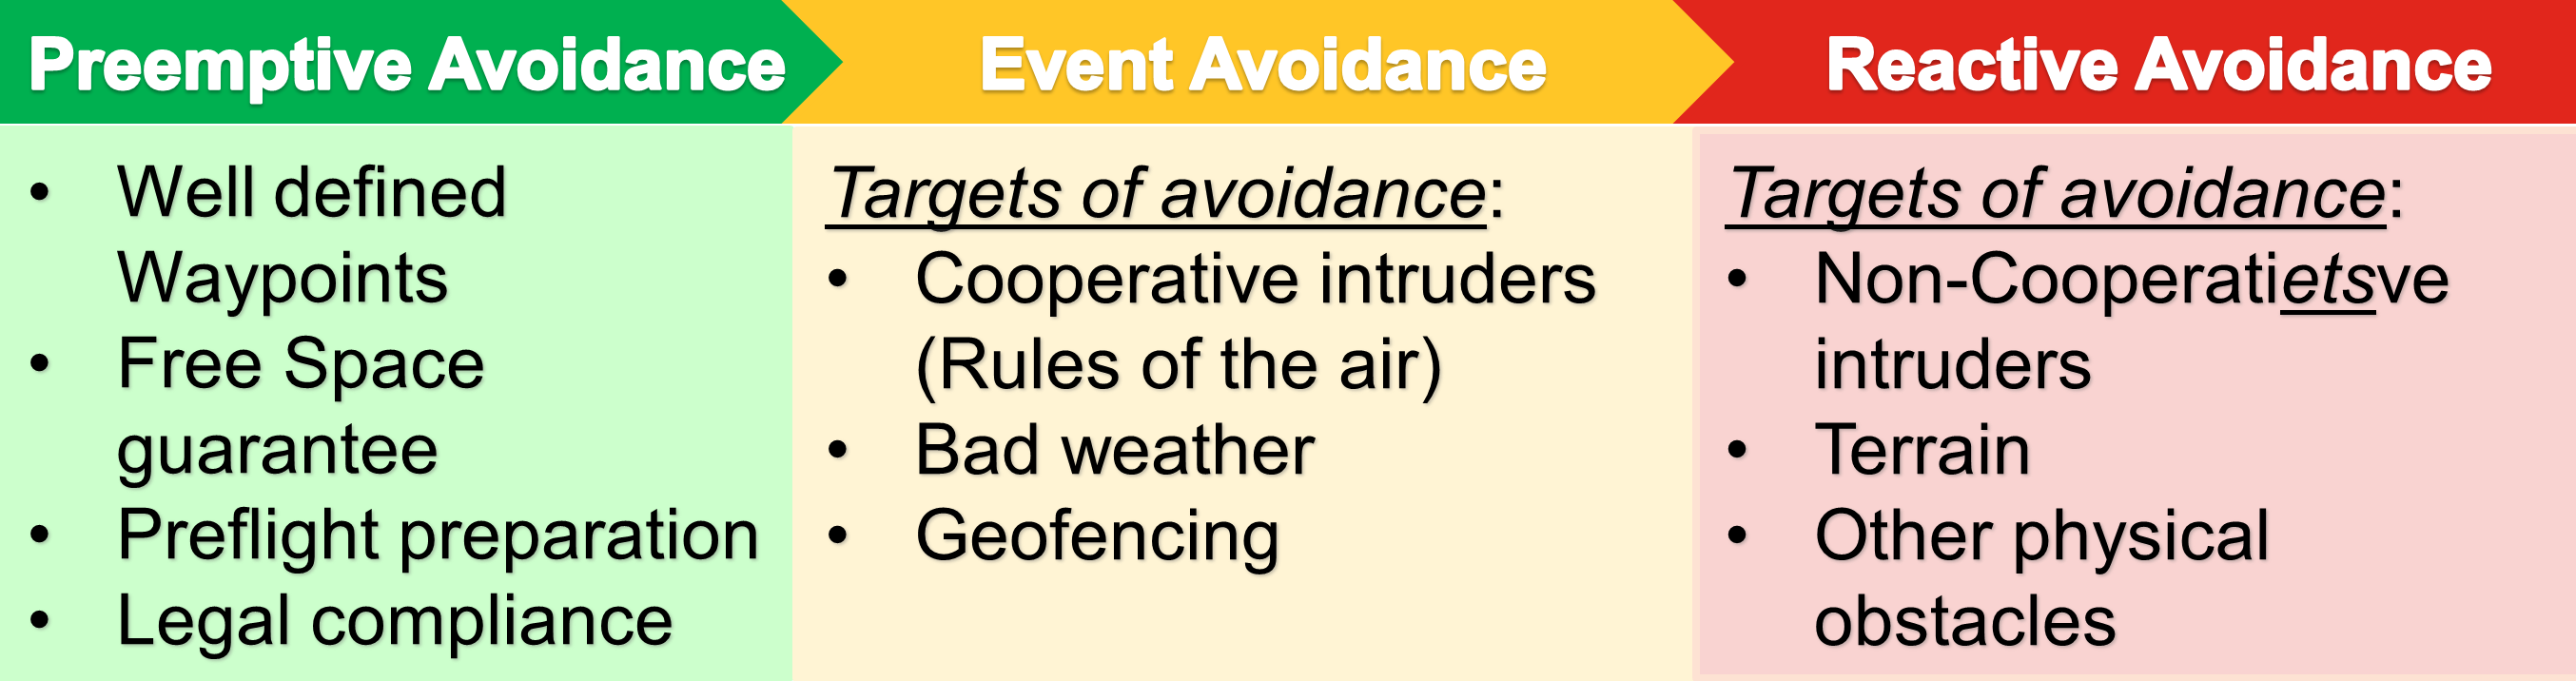
\includegraphics[width=0.7\linewidth]{\FIGDIR/RE001AvoidanceLevelsBasedOnReactionTime} 
    \caption{Avoidance levels based on reaction time.}
    \label{fig:AvoidanceLevels}
\end{figure}

\noindent This work will focus on handling \emph{Event Avoidance}, and \emph{Reactive Avoidance} and the \emph{Avoidance Path} will be calculated using \emph{Reach set Based Methods}. 

The \emph{Preemptive Avoidance} is trying to remove any possible threat before the flight. The risk mitigation is tedious and its done only when necessary. Even the best \emph{preemptive} avoidance could fail.

\emph{Reactive Avoidance} is solving most urgent situations with very short reaction opportunity. This work focus on physical obstacles and terrain. Non-cooperative intruders are partially considered. The adversary behavior was is not considered.

\emph{Event Avoidance} has more opportunity to react. Some threats are known prior the flight (geo-fenced areas, etc.). The future UTM implementation is also considered as \emph{Event Avoidance}, due to the time horizon and authority enforcement. 

\paragraph{Basic Idea:} Create deterministic finite-time \emph{Reactive Avoidance} based on \emph{Reach sets} to ensure \emph{trajectory feasibility}. Enhance method with a set of the rules to enable handling more complex situations.

The \emph{Discretization} is the key to ensure calculation in finite time. Finite \emph{partition} of \emph{operational space (Known World)} and finite representation of \emph{Reach set} guarantees finite count of calculation steps. Aircraft conflict prediction mentioned in \cite{prandini2008application}.

\newpage    
\section{Overview}\label{s:approachOverview}

\noindent The \emph{Overview} is based on \emph{Existing} Emergency avoidance framework \cite{gomola2017obstacle} (fig. \ref{fig:avoidanceConcept}). To achieve goals defined in \emph{Problem Definition} (sec. \ref{s:BasicProblemDefinition}, \ref{s:IncrementalProblemDefinition}) following \emph{Avoidance Framework Concept} (fig. \ref{fig:AvoidanceFrameworkConceptNew}) is proposed:

\begin{figure}[H]
    \centering
    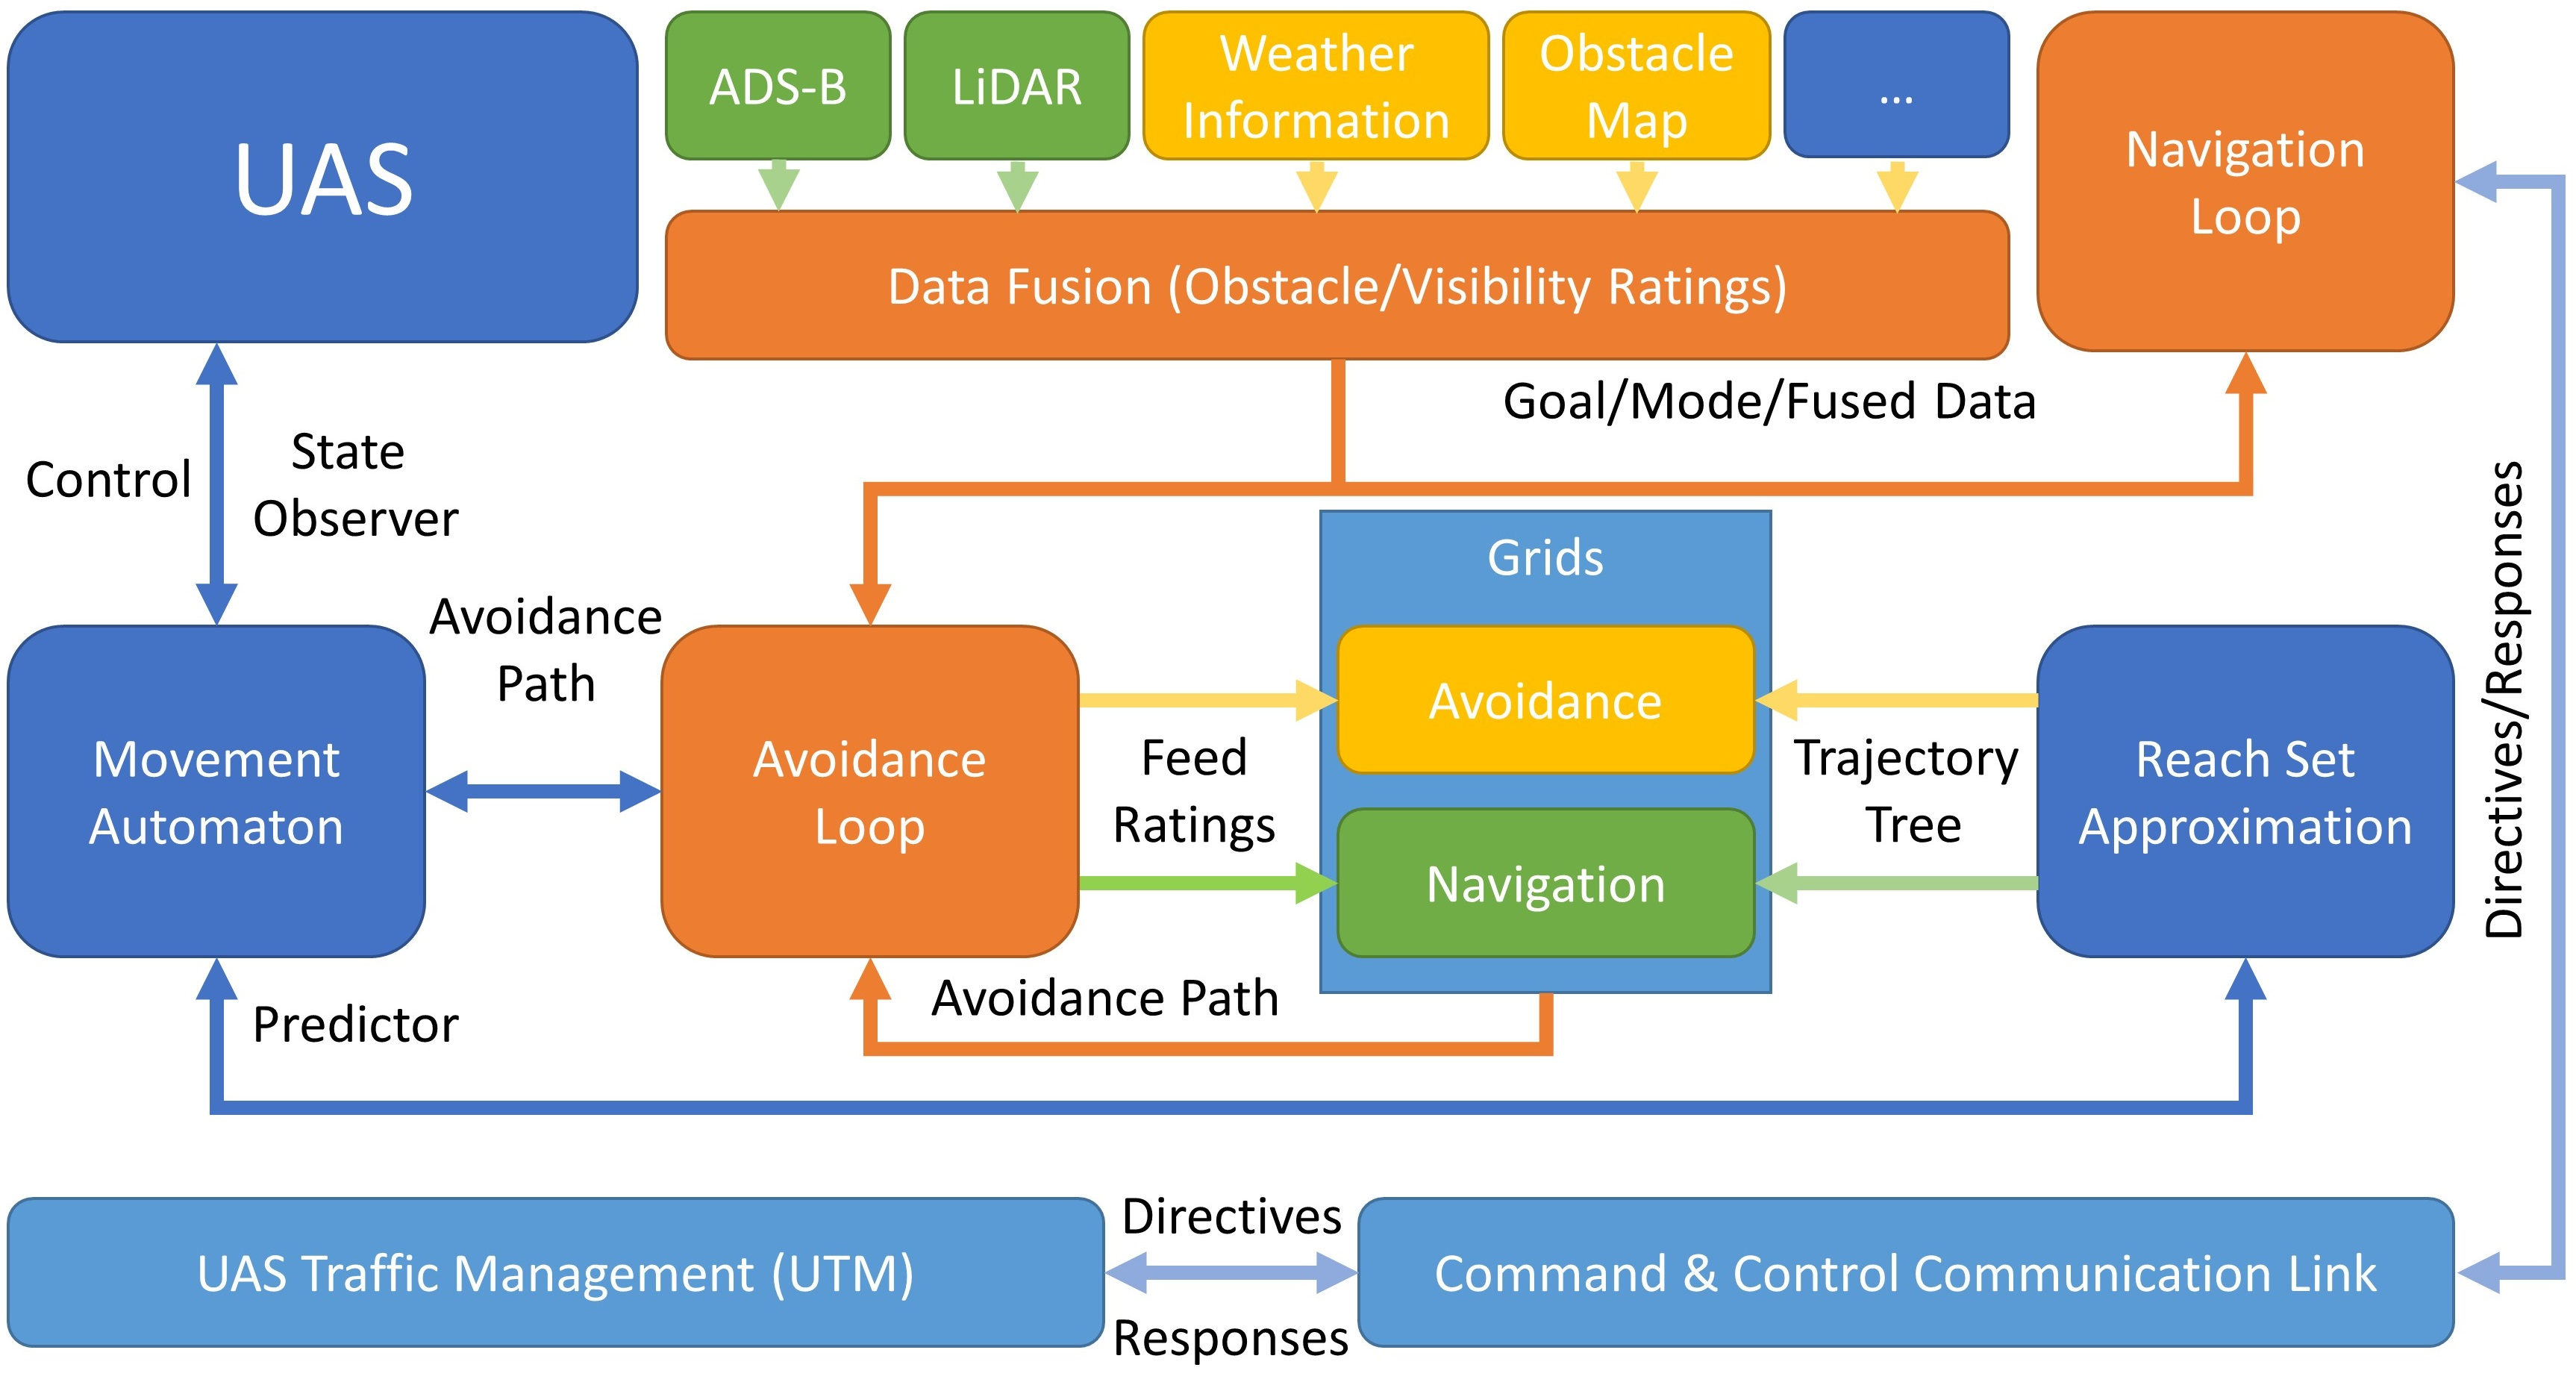
\includegraphics[width=0.95\linewidth]{\FIGDIR/TE037ConceptualSchemeNew} 
    \caption{Avoidance Framework Concept.}
    \label{fig:AvoidanceFrameworkConceptNew}
\end{figure}


\paragraph{Structure of Avoidance Framework:}

\begin{enumerate}
    \item \emph{Unmanned Aircraft System} (UAS) (Role: Controlled Plant) - the \emph{UAS} is controlled via \emph{interface} implemented as \emph{Movement Automaton}. The model used is described in (sec. \ref{s:UASNonlinearModel}).
    
    \item \emph{Movement Automaton} (Role: Control Interface/Predictor) - consumes \emph{Discrete Command Chain} to generate discrete \emph{reference trajectory}, it can  also be used as a predictor of \emph{future UAS states} (sec. \ref{s:referenceTrajectoryGenerator}). The movement Automaton used in this work is given in (sec. \ref{s:movementAutomatonDefinition}). 
    
    \item \emph{Sensor Field} (Role: Surveillance Providers), the following sensors, were considered in this work:
        \begin{enumerate}[a.]
            \item \emph{LiDAR} (Static obstacle detection) - detection of physical obstacles (eq. \ref{eq:naiveObstacleRate})
            
            \item \emph{ADS-B} (Intruder UAS/Plane detection) - detection of intruders who are broadcasting their position and sometimes heading with plans and additional parameters. The \emph{intersection models} are given in (sec. \ref{s:intruders}, app. \ref{s:linearIntersectionModel}, \ref{s:bodyvolumeIntersection}, \ref{s:uncertaintyIntersection}).
        \end{enumerate}
        
    \item \emph{Information Sources} (Role: Known World Information Enhancers): 
        \begin{enumerate}[a.]
            \item \emph{Obstacle Map} (Static Restriction Source) - imposing static soft/hard constraints on \emph{Known Word}/\emph{Operational Space}. Static constraints are given in (sec. \ref{s:virtualConstraints}).
            
            \item \emph{Weather Information} (Static/Dynamic Restriction Source) - imposing static/mo\-vi\-ng soft/hard constraints on \emph{Known World}/\emph{Operational Space}. Moving constraints are given by (def. \ref{def:movingConstraint}).
            
            \item \emph{Other Airspace Restrictions} - like restricted airspace, geo-fencing, and other future constraint sources, all of them are covered by \emph{Static/Dynamic Constraints} for now.
        \end{enumerate}
    
    \item \emph{Data Fusion} (Role: Sensor Input Interface) - is the unifying interface to asses \emph{Operational State Properties} mainly \emph{Obstacle Rating}, \emph{Visibility}, \emph{Map Obstacle Rating}, \emph{Intruder Rating} for a portion of the space. The partial \emph{ratings} are proposed in related sections. The data fusion procedure with \emph{defuzzification} and final assessment into space sets are outlined in (sec. \ref{s:sensorFusion})  
    
    \item \emph{Reach Set Approximation} (Role: Reachability Estimator) - as \emph{data fusion} is providing the situation assessment, the \emph{Reach set} is providing maneuvering capability assessment. The introduction is given in (sec. \ref{s:reachSet}), the properties are defined in (sec. \ref{s:ReachSetPerformanceCriteria}), the approximation methods with constrained expansion are outlined in (sec. \ref{s:chaoticReachSet}, \ref{s:harmonicReachSet}, \ref{s:combinedReachSet}, \ref{s:acasReachSet}). The reach set estimation is the main contribution of this work.
    
    \item \emph{Grids: Navigation/Avoidance} (Role: Operation Space Segmentation \& Situation Evaluation) - space discretization in polar coordinates grid, different reach sets are used for different grid type, defined in (sec. \ref{s:AvoidanceGrid}).
    
    \item \emph{Avoidance loop} (Role: Short Term Decision Maker) - using data from \emph{Sensor fusion} in \emph{Avoidance/Navigation Grid} trimming \emph{Reachable Space} approximated by \emph{Reach Set} generating feasible \emph{Avoidance Path}. \emph{Avoidance Path} is fed to controlling \emph{Movement Automaton}. The Goal is given by \emph{Navigation Loop}. Avoidance loop is given in (sec. \ref{s:aviudabceGridRun}).
    
    \item \emph{Navigation loop} (Role: Long Term Decision Maker) - using data from \emph{Avoidance Loop}, \emph{Mission plan} and \emph{UTM} directives defines the current long term navigation goal. Details are given in (sec. \ref{s:missionControlRun}).
    
    \item \emph{Command and Control Communication Link} (C2 Link) (Role: Communication Link) - standard communication link with sufficient reliability.
    
    \item \emph{UAS Traffic Management} (UTM) (Controlled Airspace Authority) - checking possible collisions and enforces counter-measurements. Details are given in (sec. \ref{sec:UASTrafficManagement}).
    
\end{enumerate}

\paragraph{Communication in Avoidance Framework:}
\begin{enumerate}
    \item \emph{UAS $\leftrightarrow$ Movement Automaton} - sharing \emph{actual system state}, commanding the UAS platform.
    
    \item \emph{Reach Set $\leftrightarrow$ Movement Automaton} - predicting a set of feasible trajectories for the given situation.
    
    \item \emph{Reach Set $\leftrightarrow$ Grids} - providing trajectory set depending on the active mode (Navigation/Emergency Avoidance).
    
    \item \emph{Avoidance Loop $\leftrightarrow$ Data Fusion} - assessing the situation in \emph{operational space} based on sensor readings/information sources.
    
    \item \emph{Avoidance Loop $\leftrightarrow$ Navigation Loop} - determining long term goal based on situation assessment and UTM directives. 
    
    \item \emph{Avoidance Loop $\to$ Grids} - feeding assessment data and constraints into selected operational space Grid.
    
    \item \emph{Grids $\to$ Avoidance Loop} - returning feasible and \emph{cost-effective} avoidance path after situation assessment and \emph{Reach set} pruning.
    
    \item \emph{Avoidance Loop $\to$ Movement Automaton} - issuing and monitoring movement commands based on actual \emph{avoidance strategy}.
    
    \item \emph{Navigation Loop $\leftrightarrow$ C2 Link $\leftrightarrow$ UTM} - communication to receive directives and send fulfillment. 
\end{enumerate}

    %06-03 Movement Automaton
    \cleardoublepage
\section{\secState{R}UAS Model and Control}\label{s:modelMAImplementation}

\noindent The key feature of \emph{Movement Automaton} is to interface \emph{continuous-control signal} as the \emph{discrete command chain}. Following topics are introduced in this section:

\begin{enumerate}
    \item \emph{UAS Nonlinear Model} (sec. \ref{s:UASNonlinearModel}) - simple plane model used in this work as \emph{controlled plant}.
    
    \item \emph{Movement Automaton} (sec. \ref{s:movementAutomatonDefinition}) - movement automaton for \emph{UAS Nonlinear Model} constructed from scratch.
    
    \item \emph{Segmented Movement Automaton} (sec. \ref{s:segmentedMovementAutomaton}) - for more complex systems the \emph{State Space} can be \emph{separated into Segments} and \emph{segment movement automaton} is used to generate \emph{thick reference trajectory}.
    
    \item \emph{Reference Trajectory Generator} (sec. \ref{s:referenceTrajectoryGenerator}) - other use of \emph{Movement Automaton} as predictor for \emph{reference trajectory calculation}.
\end{enumerate}


\subsection{\secState{R}UAS Nonlinear Model}\label{s:UASNonlinearModel}
\paragraph{Motivation:} Simplified rigid body kinematic model will be used. This model have decoupled roll, yaw and pitch angles. The focus is on \emph{reach set approximation methods}, therefore \emph{UAS model} is simplified.

\paragraph{State Vector} (eq. \ref{eq:simple3dStatevector}) defined as positional state in euclidean position in right-hand euclidean space, where \emph{x, y, z} can be abstracted as latitude, longitude, altitude.
\begin{equation}\label{eq:simple3dStatevector}
    state = \left [ x,y,z, roll, pitch, yaw \right]^T
\end{equation}


\paragraph{Input Vector} (eq. \ref{eq:simple3dInputVector}) is defined as linear velocity of UAS $v$ and angular speed of rigid body $\omega_{roll}, \omega_{pitch},\omega_{yaw}$.

\begin{equation}\label{eq:simple3dInputVector}
    input = \left [ v, \omega_{roll}, \omega_{pitch},\omega_{yaw}\right ]^T
\end{equation}


\noindent Velocity distribution function (eq. \ref{eq:simple3dvelocityDistribution})  is is defined trough standard rotation matrix  and linear velocity $v$, oriented velocity [$v_x$, $v_y$, $v_z$] given by (eq. \ref{eq:UASNonlinearModelSimple}).

\begin{equation}\label{eq:simple3dvelocityDistribution}
    \begin{bmatrix}
    v_x\\
    v_y\\
    v_z\
    \end{bmatrix}
    =
    \begin{bmatrix}
         v\cos(pitch)\cos(yaw)\\
         v\cos(pitch)\sin(yaw)\\
         -v\sin(pitch)\\
    \end{bmatrix}
\end{equation}

\paragraph{UAS Nonlinear Model} (eq. \ref{eq:UASNonlinearModelSimple}) is given by \emph{first order equations:}

\begin{equation}\label{eq:UASNonlinearModelSimple}
    \begin{aligned}
        \frac{\partial x}{\partial time} &= v\cos(pitch)\cos(yaw);\\
        \frac{\partial y}{\partial time} &= v\cos(pitch)\sin(yaw);\\
        \frac{\partial z}{\partial time} &= -v\sin(pitch);\\
    \end{aligned}\\\quad\quad
    \begin{aligned}
        \frac{\partial roll}{\partial time} &= \omega_{roll};\\
        \frac{\partial pitch}{\partial time} &= \omega_{pitch};\\
        \frac{\partial yaw}{\partial time} &= \omega_{yaw};\\
    \end{aligned}
\end{equation}

\subsection{\secState{R}Movement Automaton for UAS Model}\label{s:movementAutomatonDefinition}

\paragraph{Motivation:} An \emph{UAS Nonlinear Model} (eq. \ref{eq:UASNonlinearModelSimple}) can be modeled by \emph{Movement Automaton} (def. \ref{def:movementAutomaton}). 

\paragraph{Movement Primitives} by (def. \ref{def:MovementPrimitive})  are given as (eq. \ref{eq:movementPrimitive}). To define primitives the \emph{minimal time} is $1 s$. The \emph{maximal duration} is also $1s$. 

\begin{assumption}\label{ass:transitionTime}
    Let assume that \emph{transition time} of \emph{roll, pitch, yaw, linear velocity} is $0 s$.
\end{assumption}

Under the assumption (as. \ref{ass:transitionTime}) the \emph{movement transitions} (def. \ref{def:movementTransition}) have $0$ duration.

\begin{note}
    The assumption (as. \ref{ass:transitionTime}) can be relaxed under condition that \emph{path tracking controller exists}.
\end{note}

\paragraph{Movements} (def. \ref{def:Movement}) for \emph{fixed step} $k$ we start with discretization of the input variables.

\noindent The \emph{linear velocity} in text step is given:
\begin{equation}\label{eq:applyMovement}
    v(k+1) = v(k) +\delta v(k)
\end{equation}

\noindent The \emph{roll, pitch, yaw} for next step are given 

\begin{equation}\label{eq:applyMovement1}
    \begin{aligned}
        roll(k+1)  &= roll(k) + \delta roll(k)\\
        pitch(k+1) & = pitch(k) + \delta pitch(k)\\
        yaw(k+1) & = yaw(k) + \delta yaw(k)\\
    \end{aligned}    
\end{equation}

\noindent The $\delta v(k)$ is \emph{velocity change}, $\delta roll(k)$, $\delta pitch(k)$, $\delta yaw(k)$, are \emph{orientation changes} for current discrete step $k$. If the duration of \emph{transition} is $0 s$ (as. \ref{ass:transitionTime}) then 3D trajectory evolution in discrete time is given as: 

\begin{equation}\label{eq:applyMovement2}
    \begin{aligned}
        x(k+1)&= x(k) + v(k+1) \cos(pitch(k+1)) \cos(yaw(k+1)) & = \delta x(k)\\
        y(k+1)&= y(k) + v(k+1) \cos(pitch(k+1)) \sin(yaw(k+1)) & = \delta y(k)\\
        z(k+1)&= z(k) - v(k+1) \sin(pitch(k+1))                & = \delta z(k)\\
        time(k+1)& = time(k)+1                                & = \delta time(k)
    \end{aligned}    
\end{equation}

\noindent The $\delta x(k)$, $\delta y(k)$, $\delta z(k)$ are positional differences depending on \emph{input vector} for given discrete time $k$:
\begin{equation}\label{eq:ourImput}
    input(k) = \left[
                    \begin{gathered}
                    \delta x(k), \delta y(k), \delta z(k), \delta v (k),\\
                    \delta roll (k), \delta pitch(k), \delta yaw(k),\delta time (k)
                    \end{gathered} 
                \right]^T
\end{equation}

\noindent The \emph{state vector} for discrete time is given:
\begin{equation}\label{eq:ourState}
    state(k) = \left[
                    \begin{gathered}
                     x(k),  y(k),  z(k),  v (k),\\
                     roll (k),  pitch(k),  yaw(k), time (k)
                    \end{gathered} 
                \right]^T
\end{equation}

\noindent The nonlinear model (eq. \ref{eq:UASNonlinearModelSimple}) is then reduced to \emph{linear discrete model} (eq. \ref{eq:uasLinearDiscreteModel}) given by \emph{apply movements} function (eq. \ref{eq:applyMovement}, \ref{eq:applyMovement1}, \ref{eq:applyMovement2}).

\begin{equation}\label{eq:uasLinearDiscreteModel}
    state(k+1) = applyMovement(state(k), input(k)) 
\end{equation}

\paragraph{Movement Set} for linear discrete model (eq. \ref{eq:uasLinearDiscreteModel}) is defined as set of extreme unitary movements on main axes (tab. \ref{tab:movements1}) and diagonal axes (tab. \ref{tab:movements2}).

\begin{table}[H]
    \centering
    \begin{tabular}{r||r|r|r|r|r}
    
        $input(movement)$           &    Straight  & Down & Up & Left  & Right   \\\hline\hline
        $\delta     x(k)[m]$           &    1.00	  & 0.98  & 0.98  & 0.98 & 0.98  \\\hline
        $\delta     y(k)[m]$           &    0	      & 0	  & 0	  & 0.13 & -0.13 \\\hline
        $\delta     z(k)[m]$           &    0	      & -0.13 & 0.13  &	0	 & 0     \\\hline
        $\delta  roll(k) [^\circ]$	   &    0	      & 0	  & 0	  & 0    & 0     \\\hline
        $\delta pitch(k) [^\circ]$     &    0	      & $15^\circ$  & -$15^\circ$ & 0	 & 0     \\\hline
        $\delta   yaw(k) [^\circ]$     &    0	      & 0	  & 0	  & $15^\circ$ & -$15^\circ$ \\
    \end{tabular}
    \caption{Input values for main axes movements.}
    \label{tab:movements1}
\end{table}
\begin{table}[H]
    \centering
    \begin{tabular}{r||r|r|r|r}
        $input(movement)$             & Down-Left & Down-Right & Up-Left  & Up-Right   \\\hline\hline
        $\delta     x(k)[m]$           & 0.76  & 0.76  & 0.76 & 0.76  \\\hline
        $\delta     y(k)[m]$           & -0.13	& 0.13	& 0.13 & -0.13 \\\hline
        $\delta     z(k)[m]$           & -0.13 & -0.13 & 0.13 & 0.13  \\\hline
        $\delta  roll(k) [^\circ]$	& 0	    & 0	    & 0    & 0     \\\hline
        $\delta pitch(k) [^\circ]$     & -$15^\circ$ & -$15^\circ$ & $15^\circ$ & $15^\circ$     \\\hline
        $\delta   yaw(k) [^\circ]$    & $15^\circ$	& -$15^\circ$	& $15^\circ$ & -$15^\circ$ \\
    \end{tabular}
    \caption{Input values for diagonal axes movements.}
    \label{tab:movements2}
\end{table}

\begin{note}
    \emph{Movement set} in shorten form is given as
    \begin{equation}\label{eq:OurMovementSet}
        Movement Set= \left\{
        \begin{gathered}
            Straight, Left,Right, Up, Down,\\
            Down Left, Down Right,  Up Left,   Up Right
        \end{gathered}
        \right\}
    \end{equation}
\end{note}

\paragraph{Trajectory} by (def. \ref{def:MovementAutomatonTrajectory}) for initial time $time = 0$ , initial state $state(0)$ and \emph{Movement Buffer} (from def. \ref{def:MovementBuffer}):
\begin{equation}\label{eq:ourBuffer}
    Buffer \in Movement Set^* (eq. \ref{eq:OurMovementSet}), \quad  |Buffer| \in \N
\end{equation}

\noindent Trajectory (eq. \ref{eq:ourTrajectoryImplementation}) is then given as the time-series of discrete states:
\begin{equation}\label{eq:ourTrajectoryImplementation}
    Trajectory(state(0),Buffer)= \left\{\begin{gathered}state(0)+\sum_{j=0}^{i-1} input(movement(j)):\\i \in\left\{1\dots |Buffer|+1\right\}, \\movement(\cdot) \in Buffer\end{gathered}\right\}
\end{equation}

\noindent Trajectory (eq. \ref{eq:ourTrajectoryImplementation}) is ordered set of states bounded to discrete time $0\dots n$ , where $n$ is member count of \emph{Buffer}. Trajectory set has $n+1$ members:

\begin{equation}
    \begin{aligned}
    T&rajectory(state(0),Buffer)=\\
        &\left\{
        \begin{aligned}
            state(0) &= state(0) + \{\}\\
            state(1) &= state(0) + input(movement(1))\\
            state(2) &= state(0) + input(movement(1)) +input(movement(2))\\
             \vdots  &= \vdots\\
            state(n) &= state(0) + input(movement(1))+\dots+input(movement(n))\\
        \end{aligned}
        \right\}
    \end{aligned}
\end{equation}

\paragraph{State Projection} (eq. \ref{eq:ourStateProjection}) for the \emph{Trajectory} (eq. \ref{eq:ourTrajectoryImplementation}) is given as follow:
\begin{equation}\label{eq:ourStateProjection}
    StateProjection(Trajectory,time) = Trajectory.getMemberByIndex(time+1)
\end{equation}

\begin{note}
    \emph{Movement Automaton} for system (eq. \ref{eq:UASNonlinearModelSimple}) with given (as. \ref{ass:transitionTime}) is established with all related properties (sec. \ref{def:movementAutomaton}).
\end{note}

\newpage
\subsection{\secState{R}Segmented Movement Automaton}\label{s:segmentedMovementAutomaton}
\paragraph{Motivation:} Constructing \emph{Movement Automaton} for more complex system can be tedious. Used \emph{Movement Automaton} for \emph{UAS system} (\ref{eq:UASNonlinearModelSimple}) has decoupled control which is not true for most of the copters/planes \cite{fossen2011mathematical}.

\paragraph{Partitioning UAS State Space:} Proposed movement automaton is defined by its Movement set (tab. \ref{tab:movements1},\ref{tab:movements2}). Those can be scaled depending on maneuverability in the  \emph{Initial state} $state(0)$:
\begin{enumerate}
    \item \emph{Climb/Descent Rate} $\delta pitch_{max}(k)$ - the maximal climb or descent rate for Up/Down movements.
    \item \emph{Turn Rate} $\delta yaw_{max}(k)$ - the maximal turn rate for Left/Right movement.
    \item \emph{Acceleration} $\delta v_{max}(k)$ - the maximal acceleration in cruising speed range.
\end{enumerate}

\begin{definition}{State Space partition}\label{def:stateSpacePartition}
    \emph{Maneuverability} is depending on \emph{Initial State}. There can not be the infinite count of \emph{Movement Automatons}.
    
    The state space $State Space \in \R^n$ can be separated into two exclusive subsets:
    \begin{equation}
        StateSpace = [ImpactStates, NonImpactingStates]
    \end{equation}
    
    The \emph{Impacting states} are states which bounds the \emph{Maneuverability}: $\delta pitch_{max}(k)$, $\delta yaw_{max}(k)$, $\delta v_{max}(k)$. For each \emph{impact state} is possible to define upper and lower boundary:
    \begin{multline}
        \forall impactState\in ImpactStates, \exists:\\ lower(impactState) \le value(impactState) \le upper(impactState) 
    \end{multline}
    
	\noindent    The bounded interval of impact state can be separated into distinctive \emph{impact state segments} like follow:
    \begin{multline}
        impactState\in [lower,upper]:\\ \{[lower,separator_1[\dots\cup\dots[separator_i,separator_{i+1}[\dots\cup\dots\\\dots\cup\dots[separator_n,upper]\}=\\
        = impactStateIntervals(impactState)
    \end{multline}
    \begin{note}
        The interval length depends on model dynamics. The rule of thumb is to keep maximal climb/descend/turn/acceleration rates near constant value. 
    \end{note}
        
\noindent When partitioning of \emph{all impact States} finishes, the count of partitions is given as product of \emph{count of partitions} for each member of \emph{Impact States}:
    
    \begin{equation}
        partition Count = \prod_{impactState \in}^{ImpactStates} |impactStateIntervals(impactState)| 
    \end{equation}
    
    \begin{note}
        Try to keep the count of partitions to minimum, each new interval increases the count of partitions geometrically. 
    \end{note}
    
    There is finite number $n$ of \emph{Impacting States}, these are separated into $impactState-$ $Intervals_i$ with respective index $i \in 1\dots n$. The \emph{segment} with index defining position used \emph{impacting state} intervals is given as \emph{constrained space}:
    
    \begin{equation}
        Segment(index) = \left[
            \begin{gathered}
                impactState_1 \in impactStateIntervals_1[index_1],\\
                \vdots\\
                impactState_n \in impactStateIntervals_n[index_n],\\
                \vdots\\
                NonImpactingStates    
                \end{gathered}\right]
    \end{equation}
    
    Each \emph{Segment} covers one of impacting state intervals combination, because the original intervals are exclusive, also \emph{Segments} are exclusive. The \emph{union} of all segments covers \emph{State Space}:
    
    \begin{equation}\label{eq:segmentedStateSpace}
        StateSpace = \bigcup_{\forall\quad index \in |impactStateIntervals|^n} Segment(index)
    \end{equation}
\end{definition}

\paragraph{Segmented Movement Automaton:} The segmentation of \emph{state space} is done  in (def. \ref{def:stateSpacePartition}) any \emph{state} belongs exactly to \emph{Segment} of \emph{State Space}. For each \emph{Segment} in \emph{State Space}it is possible to assess: \emph{Climb/Descent Rate} $\delta pitch_{max}(k)$, \emph{Turn Rate} $\delta yaw_{max}(k)$, and, \emph{Acceleration} $\delta v_{max}(k)$.


\begin{definition}{Movement Automaton for Segment(index)}\label{def:segmentMovementAutomaton}
    

\noindent For for Model(eq. \ref{eq:uasLinearDiscreteModel}) with State (eq. \ref{eq:ourState}) the input vector (eq. \ref{eq:ourImput}) is for position $[x,y,z]$ and velocity defined like: 

\begin{equation}
    \begin{aligned}
        \delta x(k)& = \left(v(k)+\delta v(k)\right) \cos(\delta pitch(k)) \cos(\delta yaw(k))\\
        \delta y(k)& = \left(v(k)+\delta v(k)\right) \cos(\delta pitch(k)) \sin(\delta yaw(k))\\
        \delta z(k)& = -\left(v(k)+\delta v(k)\right)\cos(\delta pitch(k))\\
        \delta v(k)&\in [-\delta v(k)_{max},\delta v(k)_{max}]
    \end{aligned}
\end{equation}
\end{definition}

\noindent The acceleration $\delta v(k)$ is in interval $[-\delta v(k)_{max},\delta v(k)_{max}]$, usually set to 0 $ms^{-1}$. The change of the orientation angles for \emph{Movement Set} (eq. \ref{eq:OurMovementSet}) is given in (tab. \ref{tab:movements3},\ref{tab:movements4}).

\begin{table}[H]
    \centering
    \begin{tabular}{r||r|r|r|r|r}
    
        $input(movement)$           &    Straight  & Down & Up & Left  & Right   \\\hline\hline
        $\delta  roll(k) [^\circ]$	   &    0	      & 0	  & 0	  & 0    & 0     \\\hline
        $\delta pitch(k) [^\circ]$     &    0	      & $\delta pitch_{max}$  & -$\delta pitch_{max}$ & 0	 & 0     \\\hline
        $\delta   yaw(k) [^\circ]$     &    0	      & 0	  & 0	  & $\delta yaw_{max}$ & -$\delta yaw_{max}$ \\
    \end{tabular}
    \caption{Orientation input values for main axes movements.}
    \label{tab:movements3}
\end{table}


\begin{table}[H]
    \centering
    \begin{tabular}{r||r|r|r|r}
        $input(movement)$             & Down-Left & Down-Right & Up-Left  & Up-Right   \\\hline\hline

        $\delta  roll(k) [^\circ]$	& 0	    & 0	    & 0    & 0     \\\hline
        $\delta pitch(k) [^\circ]$     & -$\delta pitch_{max}$ & -$\delta pitch_{max}$ & $\delta pitch_{max}$ & $\delta pitch_{max}$     \\\hline
        $\delta   yaw(k) [^\circ]$    & $\delta yaw_{max}$	& -$\delta yaw_{max}$	& $\delta yaw_{max}$ & -$\delta yaw_{max}$ \\
    \end{tabular}
    \caption{Orientation input values for diagonal axes movements.}
    \label{tab:movements4}
\end{table}

\begin{note}
    The \emph{Trajectory} is calculated same as in (eq. \ref{eq:ourTrajectoryImplementation}). The \emph{State Projection} is given as in (eq. \ref{eq:ourStateProjection}).
\end{note}

\noindent Then the \emph{Movement Automaton} for \emph{Segment} $\in$ \emph{State Space} is defined.

\begin{definition}{Segmented Movement Automaton}\label{def:segmentedMovementAutomaton}
    For system with segmented state space (eq. \ref{eq:segmentedStateSpace}) there is for each $state(k)$ in $StateSpace$ injection function:
    \begin{equation} \label{eq:activeMovementAutomaton}
        ActiveMovementAutomaton:StateSpace\to MovementAutomaton
    \end{equation}
    
\noindent Selecting appropriate \emph{movement automaton} implementation (def. \ref{def:segmentMovementAutomaton}) for \emph{state(k)} $\in$ \emph{Segment} $\subset$ \emph{State Space}. The mapping function (eq. \ref{eq:activeMovementAutomaton}) is injection mapping every state(k) to Segment then \emph{Movement Automaton Implementation}. The trajectory generated is then given:
    
    \begin{equation}\label{eq:ourTrajectoryImplementationSegmented}
        Trajectory\left(\begin{gathered}state(0),\\Buffer\end{gathered}\right)= 
        \left\{
            \begin{gathered}
                state(0)+\dots\\\sum_{j=0}^{i-1} 
                    \begin{aligned} 
                        &ActiveMovementAutomaton(state(j-1)).\\
                        &\quad.input(movement(j))
                    \end{aligned}:\\
                i \in\left\{1\dots |Buffer|+1\right\}, \\
                movement(\cdot) \in Buffer
            \end{gathered}
        \right\}
    \end{equation}
    
\end{definition}

\newpage
\subsection{\secState{R}Reference Trajectory Generator}\label{s:referenceTrajectoryGenerator}

\paragraph{Reference Trajectory Generator:} Segmented Movement Automaton (def.  \ref{def:segmentedMovementAutomaton}) with \emph{trajectory function} (eq. \ref{eq:ourTrajectoryImplementationSegmented}) is used as \emph{reference trajectory generator} for \emph{complex systems}. 

There is assumption that precise \emph{path tracking} implementation exist for such system which with \emph{thick reference trajectory} gives similar results to \emph{plain movement automaton control}.

The \emph{Reference trajectory} (eq. \ref{eq:generatedReferenceTrajectory}) for \emph{Planned} movement set is given as projection  of \emph{Trajectory} time series to position time series $[x,y,z,t]$:

\begin{equation}\label{eq:generatedReferenceTrajectory}
    Reference Trajectory:Trajectory\left(\begin{gathered}state(now),\\Planned\end{gathered}\right) 
    \to 
    \begin{bmatrix}
        x_{ref} \in \R^{|Planned|}\\
        y_{ref} \in \R^{|Planned|}\\
        z_{ref} \in \R^{|Planned|}\\
        t_{ref} \in \R^{|Planned|}
    \end{bmatrix}
\end{equation}

\paragraph{Predictor:} The \emph{Reference Trajectory Generator} (eq. \ref{eq:generatedReferenceTrajectory}) can be also used as predictor. 

\begin{note}
    The \emph{Segmented Movement Automaton} (def. \ref{def:segmentedMovementAutomaton}) is used in this work with one Segment equal to State space with input function given by (\ref{tab:movements1}, \ref{tab:movements2}). The predictor used in \emph{Reach set computation} is given by (eq. \ref{eq:generatedReferenceTrajectory}).
\end{note}

    	\subsection{\secState{R}Movement Automaton Applications}\label{sec:MovementAutomatonBackground}

    \noindent\emph{Movement Automaton} is basic interface approach for discretization of \emph{trajectory evolution}  or \emph{control input} for any \emph{continuous or discrete system model}.
    
    \emph{Main function} of \emph{Movement Automaton is} for system given by equation $\dot{state}=f(time,state,input)$ with initial state $state_0$ to generate \emph{reference trajectory} $\hat{state}(t)$ or \emph{control signal} $input(t)$.
    
    Using \emph{Movement Automaton} as \emph{Control Proxy} will provide us with \emph{discrete command chain} interface. This will reduce the \emph{non deterministic} element from \emph{Evasive trajectory} generation, by reducing infinite maneuver set to finite \emph{movement set}.
    
    \emph{Non determinism} of \emph{Avoidance Maneuver} have been discussed as an issue in following works:
    \begin{enumerate}
        \item Newton gradient method for evasive car maneuvers \cite{vsantin2011combined}.
        \item Non-holistic methods for trajectory generation \cite{pin1990autonomous}.
        \item Stochastic approach to elliptic trajectories generation \cite{andrzejak2001epileptic}.
    \end{enumerate}
    
\noindent\emph{Examples} of \emph{Movement Automaton Implementation} as \emph{Control Element} can be mentioned as follows:
    \begin{enumerate}
        \item Control of traffic flow \cite{kuwata2009real}.
        \item Complex air traffic collision situation resolution system  \cite{frazzoli2001robust,frazzoli2000trajectory}.
        \item SAA/DAA capable avoidance system \cite{gomola2017obstacle}.
    \end{enumerate}



    	\section{Specialization of Hybrid Automaton}\label{s:MovementAutomatonBuidlingBlocks}

\paragraph{Idea:} There is  a need for \emph{fast trajectory approximation} method. The basic idea is taken from the pilot steering a plane. The pilot has issued commands from a navigator in a very short and precise manner. The movement has its primitive phase when steering is static, and its transition phase when steering is moving from one static position to another. 

Imagine having vertical and horizontal flaps an on airplane (fig. \ref{fig:movementsExample}). The \emph{navigator} is issuing a command every second to a pilot. Hands of the pilot translate each command to an input signal (blue line). The command validity period (black frame) is split into \emph{transition period} (red frame) when the input signal is changing and primitive period (magenta frame) when the position of the input signal is static.
 
\begin{figure}[H]
    \centering
    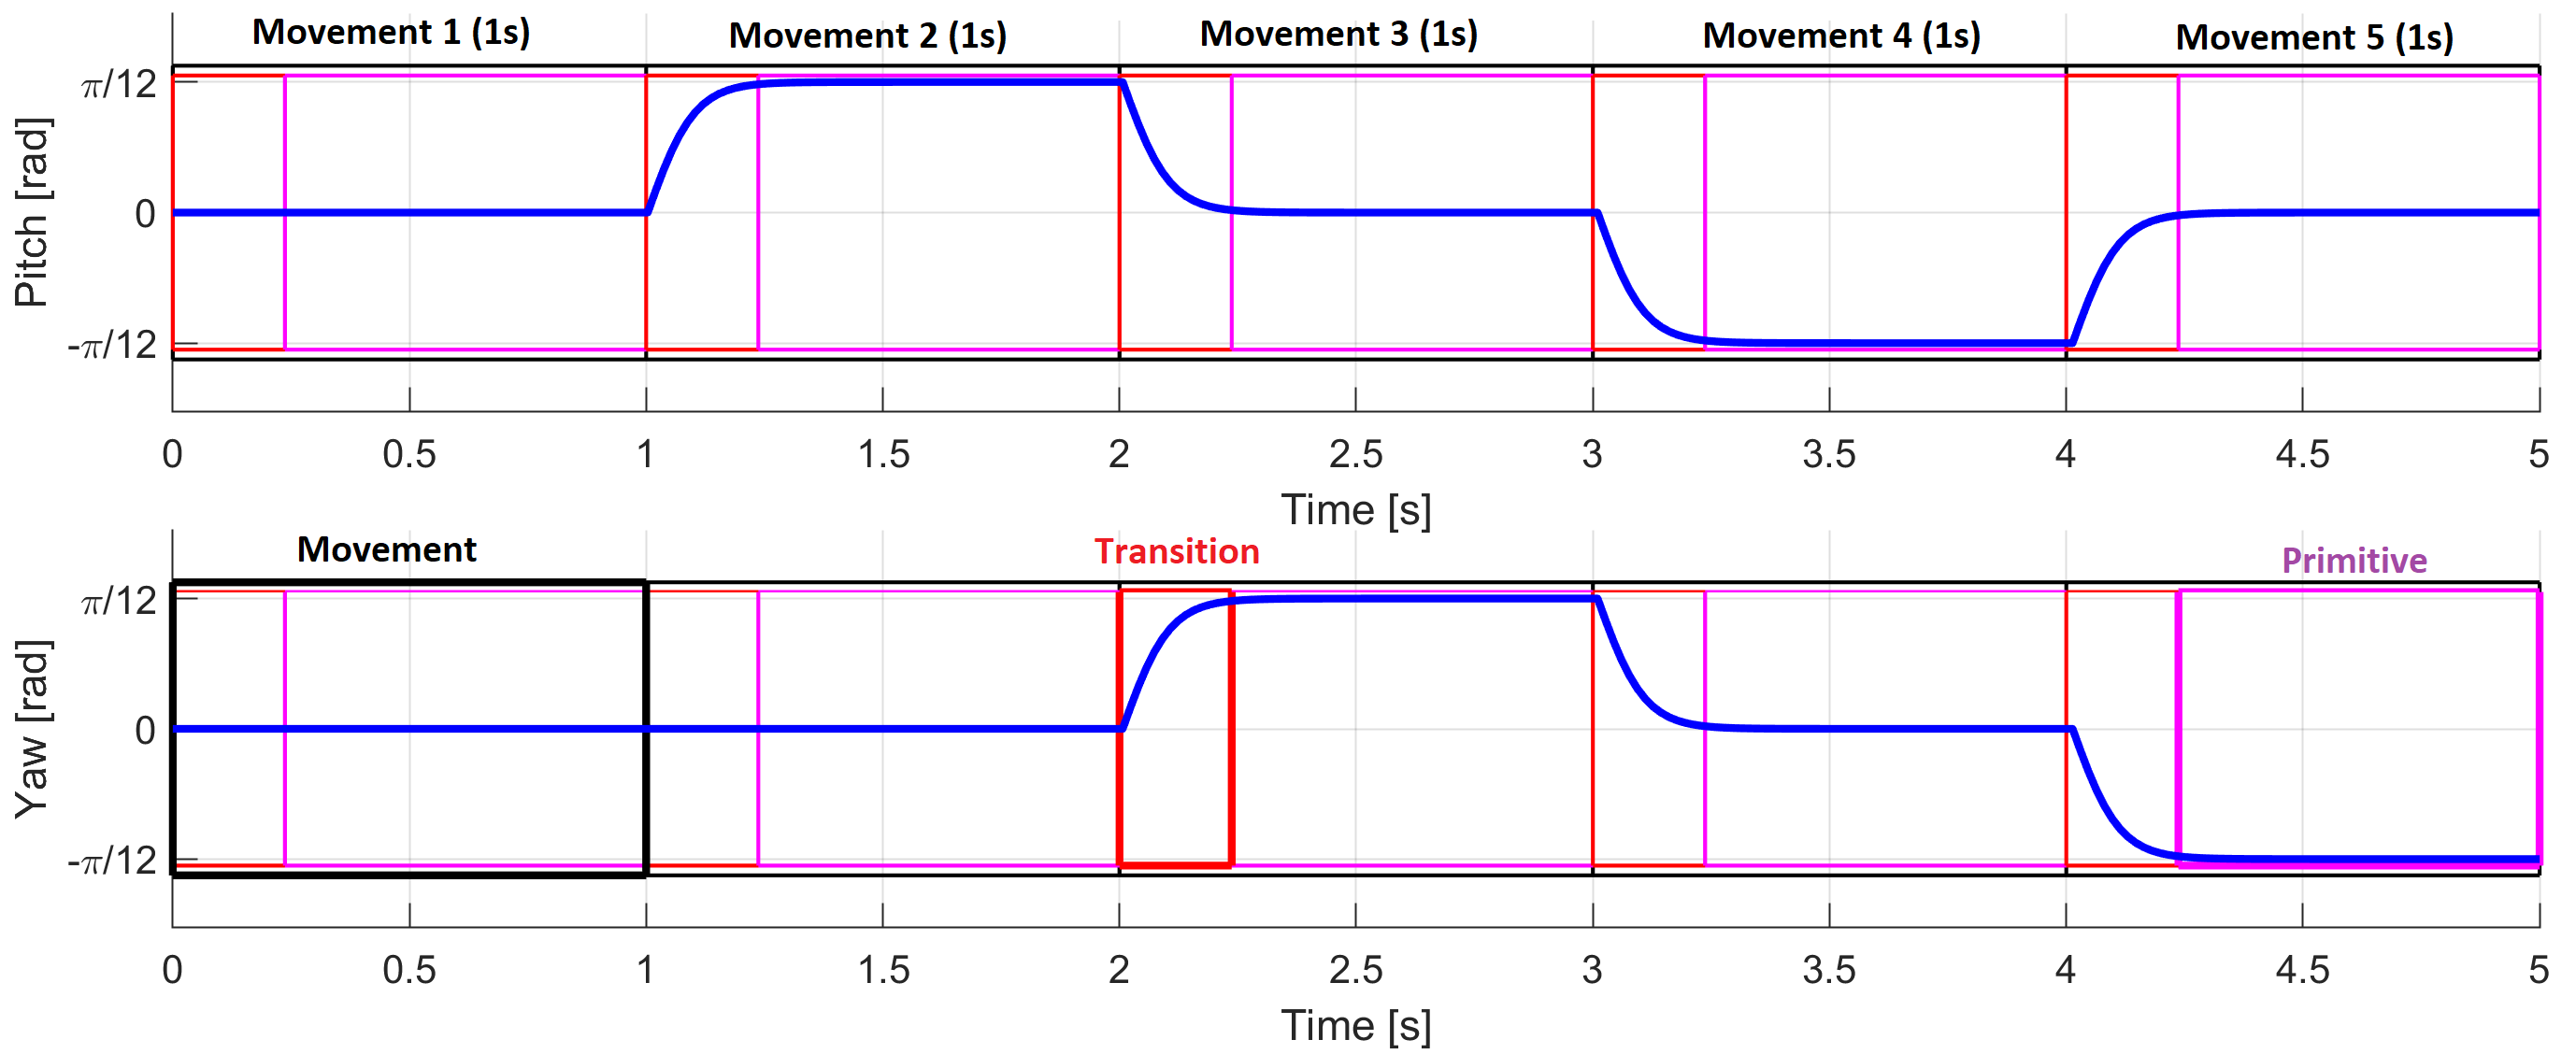
\includegraphics[width=0.95\linewidth]{\FIGDIR/TE062MovementAutomatonExampleWide} 
    \caption{Example of input signal segmentation to movements.}
    \label{fig:movementsExample}
\end{figure}

\begin{note}
    The hybrid automaton (sec. \ref{s:HybridAutomaton}) can be used as the base for simple control mechanism imitating navigators command execution by the pilot. The automaton states can be mapped to primitives and transitions. The reset map needs to be replaced with external order issuer to ensure smooth execution of commands.
    
    The future commands will be stacked in the buffer from which they will be picked for execution.
\end{note}



    \begin{definition}{Movement Primitive:}\label{def:MovementPrimitive}\\\emph{States} from \emph{Hybrid automaton} can be taken as \emph{Movements} in \emph{Movement Automaton}. \emph{MovementPrimitive} (eq. \ref{eq:movementPrimitive}) is describing the \emph{Movement} behavior as transfer function \emph{VectorField} enriched with parameters. 

    \begin{equation}\label{eq:movementPrimitive}
        \begin{aligned}
            &MovementPrimitive(vectorField,minimalDuration,parameters)\\
            &VectorField:SystemState\times parameters \to SystemState
        \end{aligned}
    \end{equation}
    \end{definition}



    \paragraph{Example: }Let say that \emph{UAS} system is given as $\dot{position}=velocity$, then let us have two \emph{MovementPrimitives}:
    
    \begin{enumerate}
        \item \textit{Stay} - $minimalTime=1s$, $parameters=\{\}$, $VectorField:\dot{position}=0$.
        \item \textit{Move} - $minimalTime=1s$, $parameters=\{velocity\}$, $VectorField:\dot{position}=velocity$.
    \end{enumerate}
    
    \paragraph{Trajectory from Movement Primitives:} The \emph{UAS} should \emph{Move} for $5s$ with velocity $10 m/s$, then \emph{Stay} for $10s$, then move for $7s$ with velocity $4 m/s$, with initial position $position_0=0$ and initial time $t_0=1$ The standard approach is to derive transfer function $position = \Theta(\dots)$
    \begin{equation}\label{eq:trajectoryExample}
        position(t)=\Theta(\dots)
        \begin{cases}
            t \in [0,5] &: 10\times t + position(0)\\
            t \in (5,15] &: 0\times (t-5) + position(5)\\
            t \in (15,22]&: 4\times (t-15) + position(15)
        \end{cases}
    \end{equation}

    The \emph{example} given by (eq. \ref{eq:trajectoryExample}) is fairly primitive, but imagine UAS system given by nonlinear dynamics \cite{fossen2011mathematical}. Then defining transfer function for a given command chain can be impossible.

    \begin{definition}{Movement Transition:}\label{def:movementTransition}\\
        \emph{System state} can be different from intended movement application, the notion of \emph{Transition} is therefore introduced as stabilizing element in movement chaining (eq. \ref{eq:movementTransition}).
        \begin{equation}\label{eq:movementTransition}
            Transition:MovementPrimitive\times SystemState \to MovementPrimitive    
        \end{equation}
    \end{definition}

    \paragraph{Trajectory with Transitions:} Introducing two transitions $Transition(Move,Stay)$ and $Transition(Stay,Move)$ reflecting periods when vehicle stop moving or speed-up to desired velocity. The transfer function (eq. \ref{eq:trajectoryExample}) can be rewritten as combination of \emph{MovementPrimitives} (eq. \ref{eq:movementPrimitive}) and \emph{Transitions} (eq. \ref{eq:movementTransition}):
    
    \begin{multline}
        Transition(Stay,Move), Move(5s,10m/s),\\
        Transition(Move,Stay), Stay(10s),\\ 
        Transition(Stay,Move), Move(7s,4m/s)
    \end{multline}.

    \begin{note} There are two types of \emph{movement primitives}:
    \begin{enumerate}
        \item \emph{Stationary} - when the system state is considered neutral, and they are considered an entry point for automaton.
        \item \emph{Dynamic} - when the system state is considered evolving, and they need to be terminated with a \emph{stationary} transition.
    \end{enumerate}
    \end{note}

    \paragraph{Movement Mapping Example:} Transition/MovementPrimitive pairs (eq. \ref{eq:movementTransition}) can be mapped into movements (eq. \ref{eq:movementMappingExample}).
    
    \begin{equation}\label{eq:movementMappingExample}
    \begin{aligned}
        Move(5s,10m/s) &:Transition(Stay,Move), Move(5s,10m/s),\\
        Stay(10s) &: Transition(Move,Stay), Stay(10s),\\ 
        Move(7s,4m/s) &: Transition(Stay,Move), Move(7s,4m/s)
    \end{aligned}    
    \end{equation}

    \begin{definition}{Movement:}\label{def:Movement}\\
        Movement can consist from multiple \emph{Transitions} (eq. \ref{eq:movementTransition}) and one \emph{MovementPrimitive} (eq. \ref{eq:movementPrimitive}), the duration of \emph{MovementPrimitive} can be shortened by \emph{Transitions} duration. \emph{Movement} is defined as follows:
        
        \begin{equation}
            \small Movement \left(
                \begin{gathered}
                    \scriptstyle initialState,\\
                    \scriptstyle initialTime[0..1],\\ 
                    \scriptstyle duration,\\ 
                    \scriptstyle parameters[0..1]
                \end{gathered}\right)
            = \small Chain \left(
            \begin{gathered}
            \small InitialTransition(\dots)[0..*],\\
            \small MovementPrimitive\left(
            \begin{gathered}
                \scriptstyle transitionState,\\
                \scriptstyle remainingDuration,\\
                \scriptstyle parameters
            \end{gathered}\right)\\
            \small LeaveTransition(\dots)[0..*],\\
            \end{gathered}
            \right)
        \end{equation}
        
        \emph{Chain function} connects multiple \emph{initial Transitions} which are applied at \emph{initialState} at \emph{initialTime}. Then own \emph{MovementPrimitive} (eq. \ref{eq:movementPrimitive}) is invoked with \emph{transitionnsState}. \emph{Transitions state} is state changed by \emph{Initial Transitions}. After \emph{Movement Primitive} there can be \emph{Leave Transitions Movement}
    \end{definition}

    \paragraph{Minimal Movement Time:} Given by (eq. \ref{eq:minimalMovementTime}) for \emph{movement} is given as the sum of \emph{MovementPrimitive} (eq. \ref{eq:movementPrimitive}) minimal time, and \emph{Transition} (eq. \ref{eq:movementTransition}) in/out combined minimal time.
    
    \begin{equation}\label{eq:minimalMovementTime}
        minimalTime(Movement)=
        \begin{aligned}
        &minimalTime(MovementPrimitive) +\\ &\text{max}_{in/out}\left\{time(Transition)\right\}
        \end{aligned}
    \end{equation}
   
    \paragraph{Movement Chaining:}\emph{Movements} can be \emph{chained} and applied to initial \emph{system state} to generate \emph{system trajectory}. Example of the trajectory is given by (eq. \ref{eq:trajectoryExample}). Movements are reversibly obtained by participation such a \emph{trajectory} into \emph{Movement primitives} and \emph{Transitions}. Then sample \emph{Trajectory} for $n\in \N^+$ movements looks like (eq. \ref{eq:movementChaining}).
    \begin{equation}\label{eq:movementChaining}
        \begin{aligned}
        &Trajectory(t_0)=State(t_0)\\
        &Trajectory(t_0,t_1]=Movement_1(Trajectory(t_0),t_0,duration_1,parameters_1)\\
        &Trajectory(t_1,t_2]=Movement_2(Trajectory(t_1),t_1,duration_2,parameters_2)\\
        &Trajectory(t_2,t_3]=Movement_3(Trajectory(t_2),t_2,duration_3,parameters_3)\\
        &\vdots\\
        &Trajectory(t_{n-1},t_n]=Movement_n(Trajectory(t_{n-1}),t_{n-1},duration_n,parameters_n)\\
        \end{aligned}
    \end{equation}

    Given \emph{Trajectory} at time $t_0$ is given as the initial \emph{State} of \emph{System}. For time interval $(t_0,t_1)$, which length is equal to $duration_1$, the \emph{State} is given by $Movement_1$ with $parameters_1$ and base time $t_0$. This behavior continues for movements $2,\dots,n$. 

    \begin{definition}{Movement Buffer:}\label{def:MovementBuffer}\\
        \noindent\emph{Movements} can be chained into \emph{Buffer} with the assumption of \emph{continuous movement execution}. \emph{Continuous movement executions} each movement in the chain (eq. \ref{eq:movementChaining}) is executed in time interval $\tau_i=(t_{i-1},t_{i}]$ where $i$ is movement order and $\forall$ $Movement_i$ starting time is $t_0$ or $t_{i-1}$ from the previous movement. With given assumption \emph{Buffer} is given as (eq. \ref{eq:movementBuffer}) with parameters $t_{i-1},t_{i}$ omitted, due $t_0$ and $duration_i$ dependency.
        
        \begin{equation}\label{eq:movementBuffer}
            Buffer = \left\{Movement_i(duration_i,parameters_i)\right\}i\in\N^+
        \end{equation}
    \end{definition}
    
    \begin{definition}{Movement Automaton Trajectory:}\label{def:MovementAutomatonTrajectory}\\
        Let say system \emph{State}$\in\R^n$ which \emph{Trajectory} is defined by movement chaining (eq. \ref{eq:movementChaining}), applied on some \emph{initial time} $t_0\in\R^+$ and final time $t_f=t_0+\sum_{i=1}^{I}duration_i$, with movements contained in \emph{Buffer} (eq. \ref{eq:movementBuffer}) is given as \emph{Trajectory} (eq. \ref{eq:TrajectoryDefinition}).
        
        \begin{equation}\label{eq:TrajectoryDefinition}
            Trajectory(t_0,State(t_0),Buffer)\text{ or } Trajectory(State_0,Buffer) \text{ if } t_0=0
        \end{equation}
    \end{definition}


    \begin{note}
        The space dimension of \emph{Trajectories} is $\R^{n+1}$ if the space dimension of state \emph{Space} is $R^n$, because \emph{Trajectory space} contains evolution of \emph{Space} in time interval $T[t_0,t_f]$.
        
        \noindent The transformation from \emph{transfer function} (eq. \ref{eq:trajectoryExample}) to \emph{trajectory} (eq. \ref{eq:TrajectoryDefinition}) is natural, only set of \emph{Movement primitives} (eq. \ref{eq:movementPrimitive}) and set of \emph{Transitions} (eq. \ref{eq:movementTransition}) is required.
    \end{note}

    \paragraph{State Projection:} \emph{Trajectory} (eq. \ref{eq:TrajectoryDefinition}) is natural evolution of space over time, then there exists \emph{StateProjection} function (eq. \ref{eq:stateprojection}) which returns \emph{State} for specific \emph{Time}.
    
    \begin{equation}\label{eq:stateprojection}
        StateProjection:Trajectory\times Time \to State(Time)
    \end{equation}


    	\newpage
\section{Formal Movement Automaton Definition}\label{s:MovementAutomatonDefinitionAndProperties}

    \begin{definition}\label{def:movementAutomaton}Movement Automaton is given as follow:
    
    \begin{align}   
        \label{eq:madInitialState}
        InitialState&: \in \R^h, h\in \N^+\\
        \label{eq:madSystemdefinition}
        System&: \dot{State}=f(Time,State,Input)\text{ or } vectorField\\
        \label{eq:madMovementPrimitive}
        Primitives &= \left\{MovementPrimitive_i\left(
                                \begin{aligned}
                                &vectorField,\\
                                &minimalDuration,\\
                                &parameters
                                \end{aligned}\right)
                            \right\} i \in \N^+\\
        \label{eq:madTransitions}
        Transitions&= \left\{Transition_j\left(
                                \begin{aligned}
                                    &MovementPrimitive_l,\\
                                    &MovementPrimitive_k
                                \end{aligned}\right)_{k\neq l}\right\} j\in N^+\\
        \label{eq:madMovements}
        Movements&= \left\{Movement_m\left[
                                \begin{aligned}
                                    &Transition_o[0..*],\\
                                    &MovementPrimitive_p\\
                                    &Transition_r[0..*],\\
                                \end{aligned}\right]_{o \neq r}\right\}  m\in N^+\\
        \label{eq:madBuffer}
        Buffer&= \left\{Movement_s(duration_s,parameters_s)\right\} s\in \N^+\\
        \label{eq:madExecuted}
        Executed&= \left\{Movement_s(duration_s,parameters_t)\right\} t\in \N^+\\
        \label{eq:madBuilder}
        Builder&:Movement \times MovementPrimitive \to Movement\\
        \label{eq:madTrajectory}
        Trajectory&:InitialState\times Movement^u \to State \times Time, u\in N^+\\
        \label{eq:madStateProjection}
        StateProjection&:Trajectory\times Time \to State(Time)  
    \end{align}
    
    \noindent \emph{System} (eq. \ref{eq:madSystemdefinition}) is given in form of \emph{differential equations} $\dot{x} = f(t,x,u)$ or \emph{other transformable equivalent}, with \emph{initial state} (eq. \ref{eq:madInitialState}).
    
    \emph{Movements} (eq. \ref{eq:movementChaining}) are defined as sequence of necessary \emph{initial transitions} (eq. \ref{eq:madTransitions}), \emph{movement primitive} (eq. \ref{eq:madMovementPrimitive}), and, \emph{leave transitions} (\ref{eq:madTransitions}).
    
    The \emph{Buffer} contains a set of \emph{movement primitives} (eq. \ref{eq:madMovementPrimitive}) to be executed in order to achieve the desired goal. \emph{Builder} (eq. \ref{eq:madBuilder}) assures that first \emph{movement primitive} (eq. \ref{eq:movementPrimitive})from \emph{Buffer} (eq. \ref{eq:madBuffer}) is transformed into \emph{next movement} (eq. \ref{eq:madMovements}) based on \emph{current movement} (eq.\ref{eq:madMovements}).
    
    \noindent The system \emph{trajectory} (eq. \ref{eq:madTrajectory}) is defined in (eq. \ref{eq:TrajectoryDefinition}). \emph{State projection} (eqs. \ref{eq:stateprojection},\ref{eq:madStateProjection}) is giving \emph{State} variable for time $t\in[t_0,t_{max}]$ where $t_max$ is given by:
    \begin{equation}
    t_{max}=t_0+\sum_{i=1,u}Buffer.Movement(i).movementDuration    
    \end{equation}
    \end{definition}
    
    \begin{note}{From Continuous Reach set to Movement Automaton Control Reach Set:}\label{eq:fromContRStoMARS}

\emph{The reach set $R$} (\ref{eq:reachSetExample1}) for system $\text{d}/\text{d} \text{t state} =model(state,input)$ with initial state $state_0=state(t_i)$ in time interval $[t_i,t_{i+1}[$  is with existing control strategy $input(t)\in Control Strategy(t)$. The reach set $R(state_0, t_0,t_1)$ where $t_1 > t_0$.
\begin{equation}\label{eq:reachSetExample1}
    R(state_0, t_0,t_1) = \bigcup \left\{state(s):input(s)\in Control Strategy(s), s\in (t_0,t_1]\right\} 
\end{equation}


\noindent\emph{The reach set $\mathscr{R}$} (\ref{eq:reachSetExample2}) of the system under the control of the \emph{movement automation} consist from the set of trajectories $Trajectory(initialState,buffer)$, which are executed in constrained time period $[t_i,t_{i+1}[$.
\begin{multline}\label{eq:reachSetExample2}
     ReachSet(state_0,t_i,t_{i+1})=\\\left\{Trajectory(state_0,buffer):\text{duration}(buffer) \le (t_{i+1}-t_i)\right\}
\end{multline}
\end{note}

\begin{note}{Weak Invariance:}

When the UAS is under the control of the movement automaton  for the obstacle avoidance problem,  by design of the avoidance algorithm, the trajectories of the UAS will not intersect any threat. This means that the controlled system $\text{d}/\text{d} \text{t state} =model(state,input)$ is \emph{weakly invariant} to the complement of the threats, and with respect to the free space. A pair $(state, SafeSpace)$, where $\text{d}/\text{d} \text{t state} =model(state,input)$ and $SafeSpace$ is a closed set, is weakly invariant if there exist controls such that a trajectory starting inside $State_0\in SafeSpace$ remains inside $State (t)\in SafeSpace$ \cite{blanchini1999set}.
 \end{note}




		\subsection{\secState{R}UAS Model}\label{s:UASNonlinearModel}
\paragraph{Motivation:} Simplified rigid body kinematic model will be used. This model have decoupled roll, yaw and pitch angles. The focus is on \emph{reach set approximation methods}, therefore \emph{UAS model} is simplified.

\paragraph{State Vector} (eq. \ref{eq:simple3dStatevector}) defined as positional state in euclidean position in right-hand euclidean space, where \emph{x, y, z} can be abstracted as latitude, longitude, altitude.
\begin{equation}\label{eq:simple3dStatevector}
    state = \left [ x,y,z, roll, pitch, yaw \right]^T
\end{equation}


\paragraph{Input Vector} (eq. \ref{eq:simple3dInputVector}) is defined as linear velocity of UAS $v$ and angular speed of rigid body $\omega_{roll}, \omega_{pitch},\omega_{yaw}$.

\begin{equation}\label{eq:simple3dInputVector}
    input = \left [ v, \omega_{roll}, \omega_{pitch},\omega_{yaw}\right ]^T
\end{equation}


\noindent Velocity vector function (eq. \ref{eq:simple3dvelocityDistribution})  is is defined through standard rotation matrix  and linear velocity $v$, oriented velocity [$v_x$, $v_y$, $v_z$] given by (eq. \ref{eq:UASNonlinearModelSimple}).

\begin{equation}\label{eq:simple3dvelocityDistribution}
    \begin{bmatrix}
    v_x\\
    v_y\\
    v_z\
    \end{bmatrix}
    =
    \begin{bmatrix}
         v\cos(pitch)\cos(yaw)\\
         v\cos(pitch)\sin(yaw)\\
         -v\sin(pitch)\\
    \end{bmatrix}
\end{equation}

\paragraph{UAS Nonlinear Model} (eq. \ref{eq:UASNonlinearModelSimple}) is given by \emph{first order equations:}

\begin{equation}\label{eq:UASNonlinearModelSimple}
    \begin{aligned}
        \frac{\text{d} x}{\text{d} time} &= v\cos(pitch)\cos(yaw);\\
        \frac{\text{d} y}{\text{d} time} &= v\cos(pitch)\sin(yaw);\\
        \frac{\text{d} z}{\text{d} time} &= -v\sin(pitch);\\
    \end{aligned}\\\quad\quad
    \begin{aligned}
        \frac{\text{d} roll}{\text{d} time} &= \omega_{roll};\\
        \frac{\text{d} pitch}{\text{d} time} &= \omega_{pitch};\\
        \frac{\text{d} yaw}{\text{d} time} &= \omega_{yaw};\\
    \end{aligned}
\end{equation}

\paragraph{Discretization} for \emph{fixed step} $k$ we start with discretization of the input variables:

\noindent The \emph{linear velocity} in text step is given:
\begin{equation}\label{eq:applyMovement}
    v(k+1) = v(k) +\delta v(k)
\end{equation}

\noindent The \emph{roll, pitch, yaw} for next step are given 

\begin{equation}\label{eq:applyMovement1}
    \begin{aligned}
        roll(k+1)  &= roll(k) + \delta roll(k)\\
        pitch(k+1) & = pitch(k) + \delta pitch(k)\\
        yaw(k+1) & = yaw(k) + \delta yaw(k)\\
    \end{aligned}    
\end{equation}

\noindent The $\delta v(k)$ is \emph{velocity change}, $\delta roll(k)$, $\delta pitch(k)$, $\delta yaw(k)$, are \emph{orientation changes} for current discrete step $k$. If the duration of \emph{transition} is $0 s$ (as. \ref{ass:transitionTime}) then 3D trajectory evolution in discrete time is given as: 

\begin{equation}\label{eq:applyMovement2}
    \begin{aligned}
        x(k+1)&= x(k) + v(k+1) \cos(pitch(k+1)) \cos(yaw(k+1)) & = \delta x(k)\\
        y(k+1)&= y(k) + v(k+1) \cos(pitch(k+1)) \sin(yaw(k+1)) & = \delta y(k)\\
        z(k+1)&= z(k) - v(k+1) \sin(pitch(k+1))                & = \delta z(k)\\
        time(k+1)& = time(k)+1                                & = \delta time(k)
    \end{aligned}    
\end{equation}

\noindent The $\delta x(k)$, $\delta y(k)$, $\delta z(k)$ are positional differences depending on \emph{input vector} for given discrete time $k$:
\begin{equation}\label{eq:ourImput}
    input(k) = \left[
                    \begin{gathered}
                    \delta x(k), \delta y(k), \delta z(k), \delta v (k),\\
                    \delta roll (k), \delta pitch(k), \delta yaw(k),\delta time (k)
                    \end{gathered} 
                \right]^T
\end{equation}

\noindent The \emph{state vector} for discrete time is given:
\begin{equation}\label{eq:ourState}
    state(k) = \left[
                    \begin{gathered}
                     x(k),  y(k),  z(k),  v (k),\\
                     roll (k),  pitch(k),  yaw(k), time (k)
                    \end{gathered} 
                \right]^T
\end{equation}


		\subsection{\secState{R}UAS Movement Automaton}\label{s:movementAutomatonDefinition}

\paragraph{Motivation:} An \emph{UAS Nonlinear Model} (eq. \ref{eq:UASNonlinearModelSimple}) can be modeled by \emph{Movement Automaton} (def. \ref{def:movementAutomaton}). 

\paragraph{Movement Primitives} by (def. \ref{def:MovementPrimitive})  are given as (eq. \ref{eq:movementPrimitive}). To define primitives the \emph{minimal time} is $1 s$. The \emph{maximal duration} is also $1s$.

\begin{note}
	Each movement primitive will last for fixed duration $1s$.
\end{note} 

\begin{assumption}\label{ass:transitionTime}
    Let assume that \emph{transition time} of \emph{roll, pitch, yaw, linear velocity} is $0 s$.
\end{assumption}

Under the assumption (as. \ref{ass:transitionTime}) the \emph{movement transitions} (def. \ref{def:movementTransition}) have zero duration. Therefore movement primitives can be considered as movements.

\begin{note}
    The assumption (as. \ref{ass:transitionTime}) can be relaxed under condition that \emph{path tracking controller exists}.
\end{note}

\paragraph{Movements} satisfying (def. \ref{def:Movement}), for the nonlinear model (eq. \ref{eq:UASNonlinearModelSimple}) reduced to \emph{discrete model} (eq. \ref{eq:uasLinearDiscreteModel}), are given by \emph{apply movements} function (eq. \ref{eq:applyMovement}, \ref{eq:applyMovement1}, \ref{eq:applyMovement2}).

\begin{equation}\label{eq:uasLinearDiscreteModel}
    state(k+1) = applyMovement(state(k), input(k)) 
\end{equation}

\paragraph{Movement Set} for discrete model (eq. \ref{eq:uasLinearDiscreteModel}) is defined as set of unitary movements on main axes (tab. \ref{tab:movements1}) and diagonal axes (tab. \ref{tab:movements2}). 

The maneuvering capability of several commercial small fixed wing UAS were merged together. The turning rate on horizontal/vertical is defined as $15^\circ$.

The deltas are posed in \emph{UAS body-fixed coordinate frame} (ap. \ref{sec:complementsOfAlgebra}) for discrete time $k$. 

\begin{table}[H]
    \centering
    \begin{tabular}{r||r|r|r|r|r}
    	\multirow{2}{*}{Parameter} & \multicolumn{5}{c}{Movement} \\\cline{2-6} 
                &    Straight  & Down & Up & Left  & Right   \\\hline\hline
        $\delta     x(k)[m]$           &    1.00	  & 0.98  & 0.98  & 0.98 & 0.98  \\\hline
        $\delta     y(k)[m]$           &    0	      & 0	  & 0	  & 0.13 & -0.13 \\\hline
        $\delta     z(k)[m]$           &    0	      & -0.13 & 0.13  &	0	 & 0     \\\hline
        $\delta  roll(k) [^\circ]$	   &    0	      & 0	  & 0	  & 0    & 0     \\\hline
        $\delta pitch(k) [^\circ]$     &    0	      & $15^\circ$  & -$15^\circ$ & 0	 & 0     \\\hline
        $\delta   yaw(k) [^\circ]$     &    0	      & 0	  & 0	  & $15^\circ$ & -$15^\circ$ \\
    \end{tabular}
    \caption{Input values for main axes movements.}
    \label{tab:movements1}
\end{table}
\begin{table}[H]
    \centering
    \begin{tabular}{r||r|r|r|r}
    	\multirow{2}{*}{Parameter} & \multicolumn{4}{c}{Movement} \\\cline{2-5} 
                    & Down-Left & Down-Right & Up-Left  & Up-Right   \\\hline\hline
        $\delta     x(k)[m]$           & 0.76  & 0.76  & 0.76 & 0.76  \\\hline
        $\delta     y(k)[m]$           & -0.13	& 0.13	& 0.13 & -0.13 \\\hline
        $\delta     z(k)[m]$           & -0.13 & -0.13 & 0.13 & 0.13  \\\hline
        $\delta  roll(k) [^\circ]$	& 0	    & 0	    & 0    & 0     \\\hline
        $\delta pitch(k) [^\circ]$     & -$15^\circ$ & -$15^\circ$ & $15^\circ$ & $15^\circ$     \\\hline
        $\delta   yaw(k) [^\circ]$    & $15^\circ$	& -$15^\circ$	& $15^\circ$ & -$15^\circ$ \\
    \end{tabular}
    \caption{Input values for diagonal axes movements.}
    \label{tab:movements2}
\end{table}

\begin{note}
    \emph{Movement set} in shorten form is given as
    \begin{equation}\label{eq:OurMovementSet}
        Movement Set= \left\{
        \begin{gathered}
            Straight, Left,Right, Up, Down,\\
            Down Left, Down Right,  Up Left,   Up Right
        \end{gathered}
        \right\}
    \end{equation}
\end{note}

\paragraph{Trajectory} by (def. \ref{def:MovementAutomatonTrajectory}) for initial time $time = 0$ , initial state $state(0)$ and \emph{Movement Buffer} (from def. \ref{def:MovementBuffer}):
\begin{equation}\label{eq:ourBuffer}
    Buffer = \left\{
                movement(j):
                \begin{aligned}
                    &movement(j)\in Movement Set (eq. \ref{eq:OurMovementSet}),\\
                    & j \in 1\dots n, n \in N^+
                \end{aligned}
            \right\}
\end{equation}

\begin{assumption}
    The buffer is always non-empty, ordered, finite list of \emph{movements}.
\end{assumption}

\begin{note}
  The buffer have finite count $n$ of movements stored. The buffer is the planning instrument used by higher level navigation/avoidance algorithm to control UAS (Control/Command interface) (fig. \ref{fig:AvoidanceFrameworkConceptNew}).
\end{note}

%\noindent Trajectory (eq. \ref{eq:ourTrajectoryImplementation}) is then %given as the time-series of discrete states:
%\begin{equation}\label{eq:ourTrajectoryImplementation}
%    Trajectory(state(0),Buffer)= \left\{\begin{gathered}state(0)+\sum_{j=0}%^{i-1} input(movement(j)):\\i \in\left\{1\dots |Buffer|+1\right\}, \%\movement(\cdot) \in Buffer\end{gathered}\right\}
%\end{equation}

The discrete trajectory (eq. \ref{eq:ourTrajectoryImplementation}) is ordered set of states bounded to discrete time $0\dots n$, where $n$ is movement count of \emph{Buffer}. Trajectory set has $n+1$ members defined like the following:

\begin{equation}
    \begin{aligned}
    T&rajectory(state(0),Buffer)=\\
        &\left\{
        \begin{aligned}
            state(0) &= state(0),\\
            state(1) &= apply Movement\left(state(0), movement(1)\right),  \\
            state(2) &= apply Movement\left(state(1), movement(2)\right),  \\
             \vdots  &= \vdots\\
            state(n-1) &= apply Movement\left(state(n-2), movement(n-1)\right),  \\
            state(n)   &= apply Movement\left(state(n-1), movement(n)\right)  \\
        \end{aligned}
        \right\}
    \end{aligned}
\end{equation}

\noindent The $apply Movement$ (eq. \ref{eq:uasLinearDiscreteModel}) is concatenation function for discrete UAS model.
		\section{\secState{R}Segmented Movement Automaton}\label{s:segmentedMovementAutomaton}
\paragraph{Motivation:} Constructing \emph{Movement Automaton} for more complex system can be tedious. Used \emph{Movement Automaton} for \emph{UAS system} (\ref{eq:UASNonlinearModelSimple}) has decoupled control which is not true for most of the copters/planes \cite{fossen2011mathematical}.

\paragraph{Partitioning UAS State Space:} Proposed movement automaton is defined by its Movement set (tab. \ref{tab:movements1},\ref{tab:movements2}). Those can be scaled depending on maneuverability in the  \emph{Initial state} $state(0)$:
\begin{enumerate}
    \item \emph{Climb/Descent Rate} $\delta pitch_{max}(k)$ - the maximal climb or descent rate for Up/Down movements.
    \item \emph{Turn Rate} $\delta yaw_{max}(k)$ - the maximal turn rate for Left/Right movement.
    \item \emph{Acceleration} $\delta v_{max}(k)$ - the maximal acceleration in cruising speed range.
\end{enumerate}

\begin{definition}{State Space partition}\label{def:stateSpacePartition}
    \emph{Maneuverability} is depending on \emph{Initial State}. There can not be the infinite count of \emph{Movement Automatons}.
    
    The state space $State Space \in \R^n$ can be separated into two exclusive subsets:
    \begin{equation}
        StateSpace = [ImpactStates, NonImpactingStates]
    \end{equation}
    
    The \emph{Impacting states} are states which bounds the \emph{Maneuverability}: $\delta pitch_{max}(k)$, $\delta yaw_{max}(k)$, $\delta v_{max}(k)$. For each \emph{impact state} is possible to define upper and lower boundary:
    \begin{multline}
        \forall impactState\in ImpactStates, \exists:\\ lower(impactState) \le value(impactState) \le upper(impactState) 
    \end{multline}
    
	\noindent    The bounded interval of impact state can be separated into distinctive \emph{impact state segments} like follow:
    \begin{multline}
        impactState\in [lower,upper]:\\ \{[lower,separator_1[\dots\cup\dots[separator_i,separator_{i+1}[\dots\cup\dots\\\dots\cup\dots[separator_n,upper]\}=\\
        = impactStateIntervals(impactState)
    \end{multline}
    \begin{note}
        The interval length depends on model dynamics. The rule of thumb is to keep maximal climb/descend/turn/acceleration rates near constant value. 
    \end{note}
      
\noindent When partitioning of \emph{all impact States} finishes, the count of partitions is given as product of \emph{count of partitions} for each member of \emph{Impact States}:
    
    \begin{equation}
        partition Count = \prod_{impactState \in}^{ImpactStates} |impactStateIntervals(impactState)| 
    \end{equation}
    
    \begin{note}
        Try to keep the count of partitions to minimum, each new interval increases the count of partitions geometrically. 
    \end{note}
    
    There is finite number $n$ of \emph{Impacting States}, these are separated into $impactState-$ $Intervals_i$ with respective index $i \in 1\dots n$. The \emph{segment} with index defining position used \emph{impacting state} intervals is given as \emph{constrained space}:
    
    \begin{equation}
        Segment(index) = \left[
            \begin{gathered}
                impactState_1 \in impactStateIntervals_1[index_1],\\
                \vdots\\
                impactState_n \in impactStateIntervals_n[index_n],\\
                \vdots\\
                NonImpactingStates    
                \end{gathered}\right]
    \end{equation}
    
    Each \emph{Segment} covers one of impacting state intervals combination, because the original intervals are exclusive, also \emph{Segments} are exclusive. The \emph{union} of all segments covers \emph{State Space}:
    
    \begin{equation}\label{eq:segmentedStateSpace}
        StateSpace = \bigcup_{\forall\quad index \in |impactStateIntervals|^n} Segment(index)
    \end{equation}
\end{definition}

\paragraph{Segmented Movement Automaton:} The segmentation of \emph{state space} is done  in (def. \ref{def:stateSpacePartition}) any \emph{state} belongs exactly to \emph{Segment} of \emph{State Space}. For each \emph{Segment} in \emph{State Space}it is possible to assess: \emph{Climb/Descent Rate} $\delta pitch_{max}(k)$, \emph{Turn Rate} $\delta yaw_{max}(k)$, and, \emph{Acceleration} $\delta v_{max}(k)$.


\begin{definition}{Movement Automaton for Segment(index)}\label{def:segmentMovementAutomaton}
    

\noindent For for Model(eq. \ref{eq:uasLinearDiscreteModel}) with State (eq. \ref{eq:ourState}) the input vector (eq. \ref{eq:ourImput}) is for position $[x,y,z]$ and velocity defined like: 

\begin{equation}
    \begin{aligned}
        \delta x(k)& = \left(v(k)+\delta v(k)\right) \cos(\delta pitch(k)) \cos(\delta yaw(k))\\
        \delta y(k)& = \left(v(k)+\delta v(k)\right) \cos(\delta pitch(k)) \sin(\delta yaw(k))\\
        \delta z(k)& = -\left(v(k)+\delta v(k)\right)\cos(\delta pitch(k))\\
        \delta v(k)&\in [-\delta v(k)_{max},\delta v(k)_{max}]
    \end{aligned}
\end{equation}
\end{definition}

\noindent The acceleration $\delta v(k)$ is in interval $[-\delta v(k)_{max},\delta v(k)_{max}]$, usually set to 0 $ms^{-1}$. The change of the orientation angles for \emph{Movement Set} (eq. \ref{eq:OurMovementSet}) is given in (tab. \ref{tab:movements3},\ref{tab:movements4}).

\begin{table}[H]
    \centering
    \begin{tabular}{r||r|r|r|r|r}
    
        $input(movement)$           &    Straight  & Down & Up & Left  & Right   \\\hline\hline
        $\delta  roll(k) [^\circ]$	   &    0	      & 0	  & 0	  & 0    & 0     \\\hline
        $\delta pitch(k) [^\circ]$     &    0	      & $\delta pitch_{max}$  & -$\delta pitch_{max}$ & 0	 & 0     \\\hline
        $\delta   yaw(k) [^\circ]$     &    0	      & 0	  & 0	  & $\delta yaw_{max}$ & -$\delta yaw_{max}$ \\
    \end{tabular}
    \caption{Orientation input values for main axes movements.}
    \label{tab:movements3}
\end{table}


\begin{table}[H]
    \centering
    \begin{tabular}{r||r|r|r|r}
        $input(movement)$             & Down-Left & Down-Right & Up-Left  & Up-Right   \\\hline\hline

        $\delta  roll(k) [^\circ]$	& 0	    & 0	    & 0    & 0     \\\hline
        $\delta pitch(k) [^\circ]$     & -$\delta pitch_{max}$ & -$\delta pitch_{max}$ & $\delta pitch_{max}$ & $\delta pitch_{max}$     \\\hline
        $\delta   yaw(k) [^\circ]$    & $\delta yaw_{max}$	& -$\delta yaw_{max}$	& $\delta yaw_{max}$ & -$\delta yaw_{max}$ \\
    \end{tabular}
    \caption{Orientation input values for diagonal axes movements.}
    \label{tab:movements4}
\end{table}

\begin{note}
    The \emph{Trajectory} is calculated same as in (eq. \ref{eq:ourTrajectoryImplementation}). The \emph{State Projection} is given as in (eq. \ref{eq:ourStateProjection}).
\end{note}

\noindent Then the \emph{Movement Automaton} for \emph{Segment} $\in$ \emph{State Space} is defined.

\begin{definition}{Segmented Movement Automaton}\label{def:segmentedMovementAutomaton}
    For system with segmented state space (eq. \ref{eq:segmentedStateSpace}) there is for each $state(k)$ in $StateSpace$ injection function:
    \begin{equation} \label{eq:activeMovementAutomaton}
        ActiveMovementAutomaton:StateSpace\to MovementAutomaton
    \end{equation}
    
\noindent Selecting appropriate \emph{movement automaton} implementation (def. \ref{def:segmentMovementAutomaton}) for \emph{state(k)} $\in$ \emph{Segment} $\subset$ \emph{State Space}. The mapping function (eq. \ref{eq:activeMovementAutomaton}) is injection mapping every state(k) to Segment then \emph{Movement Automaton Implementation}. The trajectory generated is then given:
    
    \begin{equation}\label{eq:ourTrajectoryImplementationSegmented}
        Trajectory\left(\begin{gathered}state(0),\\Buffer\end{gathered}\right)= 
        \left\{
            \begin{gathered}
                state(0)+\dots\\\sum_{j=0}^{i-1} 
                    \begin{aligned} 
                        &ActiveMovementAutomaton(state(j-1)).\\
                        &\quad.input(movement(j))
                    \end{aligned}:\\
                i \in\left\{1\dots |Buffer|+1\right\}, \\
                movement(\cdot) \in Buffer
            \end{gathered}
        \right\}
    \end{equation}
    
\end{definition}



		\section{\secState{R}Reference Trajectory Generator}\label{s:referenceTrajectoryGenerator}

\paragraph{Reference Trajectory Generator:} Segmented Movement Automaton (def.  \ref{def:segmentedMovementAutomaton}) with \emph{trajectory function} (eq. \ref{eq:ourTrajectoryImplementationSegmented}) is used as a \emph{reference trajectory generator} for \emph{complex systems}. 

There is an assumption that precise \emph{path tracking} implementation exist for such system which with \emph{thick reference trajectory} gives similar results to \emph{plain movement automaton control}.

The \emph{Reference trajectory} (eq. \ref{eq:generatedReferenceTrajectory}) for \emph{Planned} movement set is given as projection  of \emph{Trajectory} time series to position time series $[x,y,z,t]$:

\begin{equation}\label{eq:generatedReferenceTrajectory}
    Reference Trajectory:Trajectory\left(\begin{gathered}state(now),\\Planned\end{gathered}\right) 
    \to 
    \begin{bmatrix}
        x_{ref} \in \R^{|Planned|}\\
        y_{ref} \in \R^{|Planned|}\\
        z_{ref} \in \R^{|Planned|}\\
        t_{ref} \in \R^{|Planned|}
    \end{bmatrix}
\end{equation}

\paragraph{Predictor:} The \emph{Reference Trajectory Generator} (eq. \ref{eq:generatedReferenceTrajectory}) can also be used as a predictor. 

\begin{note}
    The \emph{Segmented Movement Automaton} (def. \ref{def:segmentedMovementAutomaton}) is used in this work with one Segment equal to State space with input function given by (\ref{tab:movements1}, \ref{tab:movements2}). The predictor used in \emph{Reach set computation} is given by (eq. \ref{eq:generatedReferenceTrajectory}).
\end{note}

\paragraph{State Projection} (eq. \ref{eq:ourStateProjection}) for the \emph{Trajectory} (eq. \ref{eq:ourTrajectoryImplementation}) is given as follow:
\begin{equation}\label{eq:ourStateProjection}
    StateProjection(Trajectory,time) = Trajectory.getMemberByIndex(time+1)
\end{equation}

\begin{note}
    \emph{Movement Automaton} for system (eq. \ref{eq:UASNonlinearModelSimple}) with given (as. \ref{ass:transitionTime}) is established with all related properties (sec. \ref{def:movementAutomaton}).
\end{note}
 
	
	%06-02 Avoidance Grid
	\cleardoublepage
\section{\secState{R}Space Discretization - Avoidance Grid}\label{s:AvoidanceGrid}

\paragraph{Operation Space:} The \emph{Operation Space} is a space where UAS can effectively surveillance its surroundings and it has capability to act.

\paragraph{Motivation for Discretization:} The UAS surroundings needs to be represented in \emph{avoidance-friendly manner}, following principles matters:

\begin{enumerate}
	\item \emph{Discrete representation} - the space around UAS should be segmented into finite and exclusive portions which are considered as one point of the grid. This enables fast situation assessment. 
	
	\item \emph{Threat proximity} - threat in any form is getting more important with decreasing distance to UAS.
	
	\item \emph{LiDAR swipe density} - one LiDAR swipe scans a lot of points, the grid need to be customized to swipe characteristics.
\end{enumerate}


The \emph{Main Sensor} is \emph{LiDAR} (problems \ref{eq:basicProblemDefinition}.-\ref{pro:rulesOfTheAir}).  The \emph{effective occupancy computation} needs to be done for all problems; the inspiration is taken from \cite{homm2010efficient}.  The \emph{effective occupancy computation} is done in \emph{LiDAR} scan  portioned into \emph{polar coordinates grid}. The\emph{operation space} is abstracted as\ emph{grid} where \emph{space portions} are representing the points in the grid.

\begin{note}
	Each member of the grid is a cell, represented as a point with shared properties, like threat level, visibility.
\end{note}

The \emph{Discrete Situation Evaluation} is executed for a \emph{UAS} local coordinate frame in fixed \emph{time}.  The goal is to enable \emph{fast discrete situation assessment}. 


\paragraph{LiDAR Swipe:} The \emph{point} scanned by \emph{LiDAR}, where the \emph{UAS position} is center of \emph{local coordinate frame} and \emph{UAS heading is defining the main axes} is given as:

\begin{equation}\label{eq:LiDARPoint}
    point = [distance,horizontal^\circ,vertical^\circ].
\end{equation}

\begin{note}
    For polar/euclidean transformations and local/global coordinate frames refer to background theory (app. \ref{sec:complementsOfAlgebra}). 
    
    The \emph{right side} of UAS $horizontal^\circ$ $\in$ $]-\pi,0[$, the \emph{left side} of UAS $horizontal^\circ$ $\in$ $[0,\pi]$, the \emph{down side} of UAS $vertical^\circ$ $\in$ $]-\pi,0[$, the \emph{top side} of UAS $vertical^\circ$ $\in$ $[0,\pi]$
\end{note}

\paragraph{LiDAR Swipe Portioning:} The \emph{polar coordinate space} can be portioned into distingtive cells, which contains the portion the space. This cell then represents one point in the grid.

The \emph{reason} for this swipe portioning is \emph{LiDAR} scanning density\footnote{Example rotary LiDAR Velodyne VL-16 specs: \url{https://www.cadden.fr/wp-content/uploads/2017/02/Velodyne_VLP-16-Puck.pdf}}, which is extremly dense. The \emph{threat} state in the cell can be assessed with linear complexity. 

The \emph{polar $\to$ euclidean} coordinate frame transformation is not amenable  for LiDAR swipe. The \emph{threath} assessment based on \emph{LiDAR swipe} in \emph{planar space portions} has minimal complexity and it is cost effective. \cite{gupta2010comparative}.


\paragraph{Cell:} To discretize operational space into grid of points there is a need to define cell space, which bounds the portion of \emph{local planar coordinate frame}. The point (eq. \ref{eq:LiDARPoint}) is defined by distance, horizontal$^\circ$ offset angle, and vertical$^\circ$ offset angle. The cell is a closed compact set of such points. The boundary can be defined like follow: 

\begin{definition}{Cell}\label{def:cell}
	
    \noindent The \emph{cell} bounds a portion of space in UAS local polar coordinate frame, defined by boundary ranges:
    \begin{enumerate}
        
        \item \emph{Distance Range} -  starts and ends: $distance_{start}$ $<$ $distance_{end}$ $in$ $\R^+$.
        
        \item \emph{Horizontal Range} - starts and ends: $horizontal^\circ_{start}$ $<$ $horizontal^\circ_{end}$ $\in$ $]-\pi,\pi]$.
        
        \item \emph{Vertical Range} - starts and ends: by $vertical^\circ_{start}$ $<$ $vertical^\circ_{end}$ $\in$ $]-\pi,\pi]$.
    \end{enumerate}
    
    \noindent The \emph{space portion} belonging to the \emph{cell} is given by function as:
    
    \begin{multline}\label{eq:boundedSpaceCell}
        cell.space Portion\dots\\
            \left \{
                \begin{aligned}
                point& \in \R^3 \text{ where}:\\
                    &\left(\begin{aligned}
                        cell.distance_{start} &<& point.distance &\le& cell.distance_{end},\\
                        cell.horizontal^\circ_{start} &<& point.horizontal^\circ &\le&  cell.horizontal^\circ_{end},\\
                        cell.vertical^\circ_{start} &<& point.vertical^\circ &\le& cell.vertical^\circ_{end}\\
                    \end{aligned}\right)
                \end{aligned}
            \right\}
    \end{multline}
    
    \noindent To evaluate \emph{static obstacle threat}, it is necessary to know how many LiDAR hits landed in cell space portion. For one \emph{LiDAR Scan} the \emph{hits set} is given as \emph{set} of \emph{all points} which lands into cell space portion:
    \begin{equation}\label{eq:LidarHitsCell}
        cell. LiDAR Hits = \left\{point \in Lidar Scan:  point \in cell. space Portion\right\}    
    \end{equation}
    
    %\noindent The \emph{passing hits} for cell are hits which are going through the cell (passing), but it lands in distance greater than $cell.distance_{end}$, defined as:
%    \begin{multline}\label{eq:passingHitsCell}
%        Passing Hits(cell)=
%        \dots\\
%            \left \{
%                \begin{aligned}
%                point& \in Lidar Scan \text{ where}:\\
%                    &\left(\begin{aligned}
%                        cell.distance_{end}&<& point.distance &&,\\
%                        cell.horizontal^\circ_{start} &<& point.horizontal^\circ &\le&  %cell.horizontal^\circ_{end},\\
%                        cell.vertical^\circ_{start} &<& point.vertical^\circ &\le& %cell.vertical^\circ_{end}\\
%                    \end{aligned}\right)
%                \end{aligned}
%            \right\}
%    \end{multline}
\end{definition}

\begin{note}
    The \emph{cell} space portion volume is increasing with the distance. This satisfy the requirement for threat-distance importance.  The cell is considered as a point of grid with common properties abstraction valid for all cell space portion.    
\end{note}

\paragraph{Effective Operation Space:} The goal is to determine which of the operation space is going to be considered in our avoidance grid.  The effective operation space determination according to \cite{zaiane2002clustering} is influenced by the following factors:

\begin{enumerate}
        \item \emph{Sensors ranges} -  there is no reason to assess situation over effective \emph{sensor range}.
        
        \item \emph{Information sources} impact - there is no real impact on \emph{effective space boundary}, the information search and intersection algorithms are only of the importance.
        
        \item \emph{UAS maneuverability} - the space where UAS can maneuver, bounded by space-time (reach set boundary). 
        
        \item \emph{Computation power} - the situation evaluation and threat assessment capabilities of onboard computer.
        
        \item \emph{Airworthiness requirements} - the \emph{regulations} can impose some minimal requirements on \emph{effective operation space boundary}.
\end{enumerate}

Let show an example of \emph{effective operation space} for the UAS  (fig. \ref{fig:LidarSpaceSegmentation}).  The \emph{full LiDAR Swipe} (cyan and red lines) of \emph{UAS} (blue plane) has \emph{shape} of conical cylinder. 

\begin{note}
Under \emph{ideal circumstances} the \emph{LiDAR swipe} would have \emph{ball shape}, but in real cases the \emph{UAS body portion} where \emph{LiDAR} is mounted is unused.
\end{note}

The \emph{frontal portion} (red line) is a set of cells where \emph{UAS} can make maneuvers. According to the \emph{previous conditions}, there is no reason to consider space portion out of the maneuverable area. 

\begin{figure}[H]
    \centering
    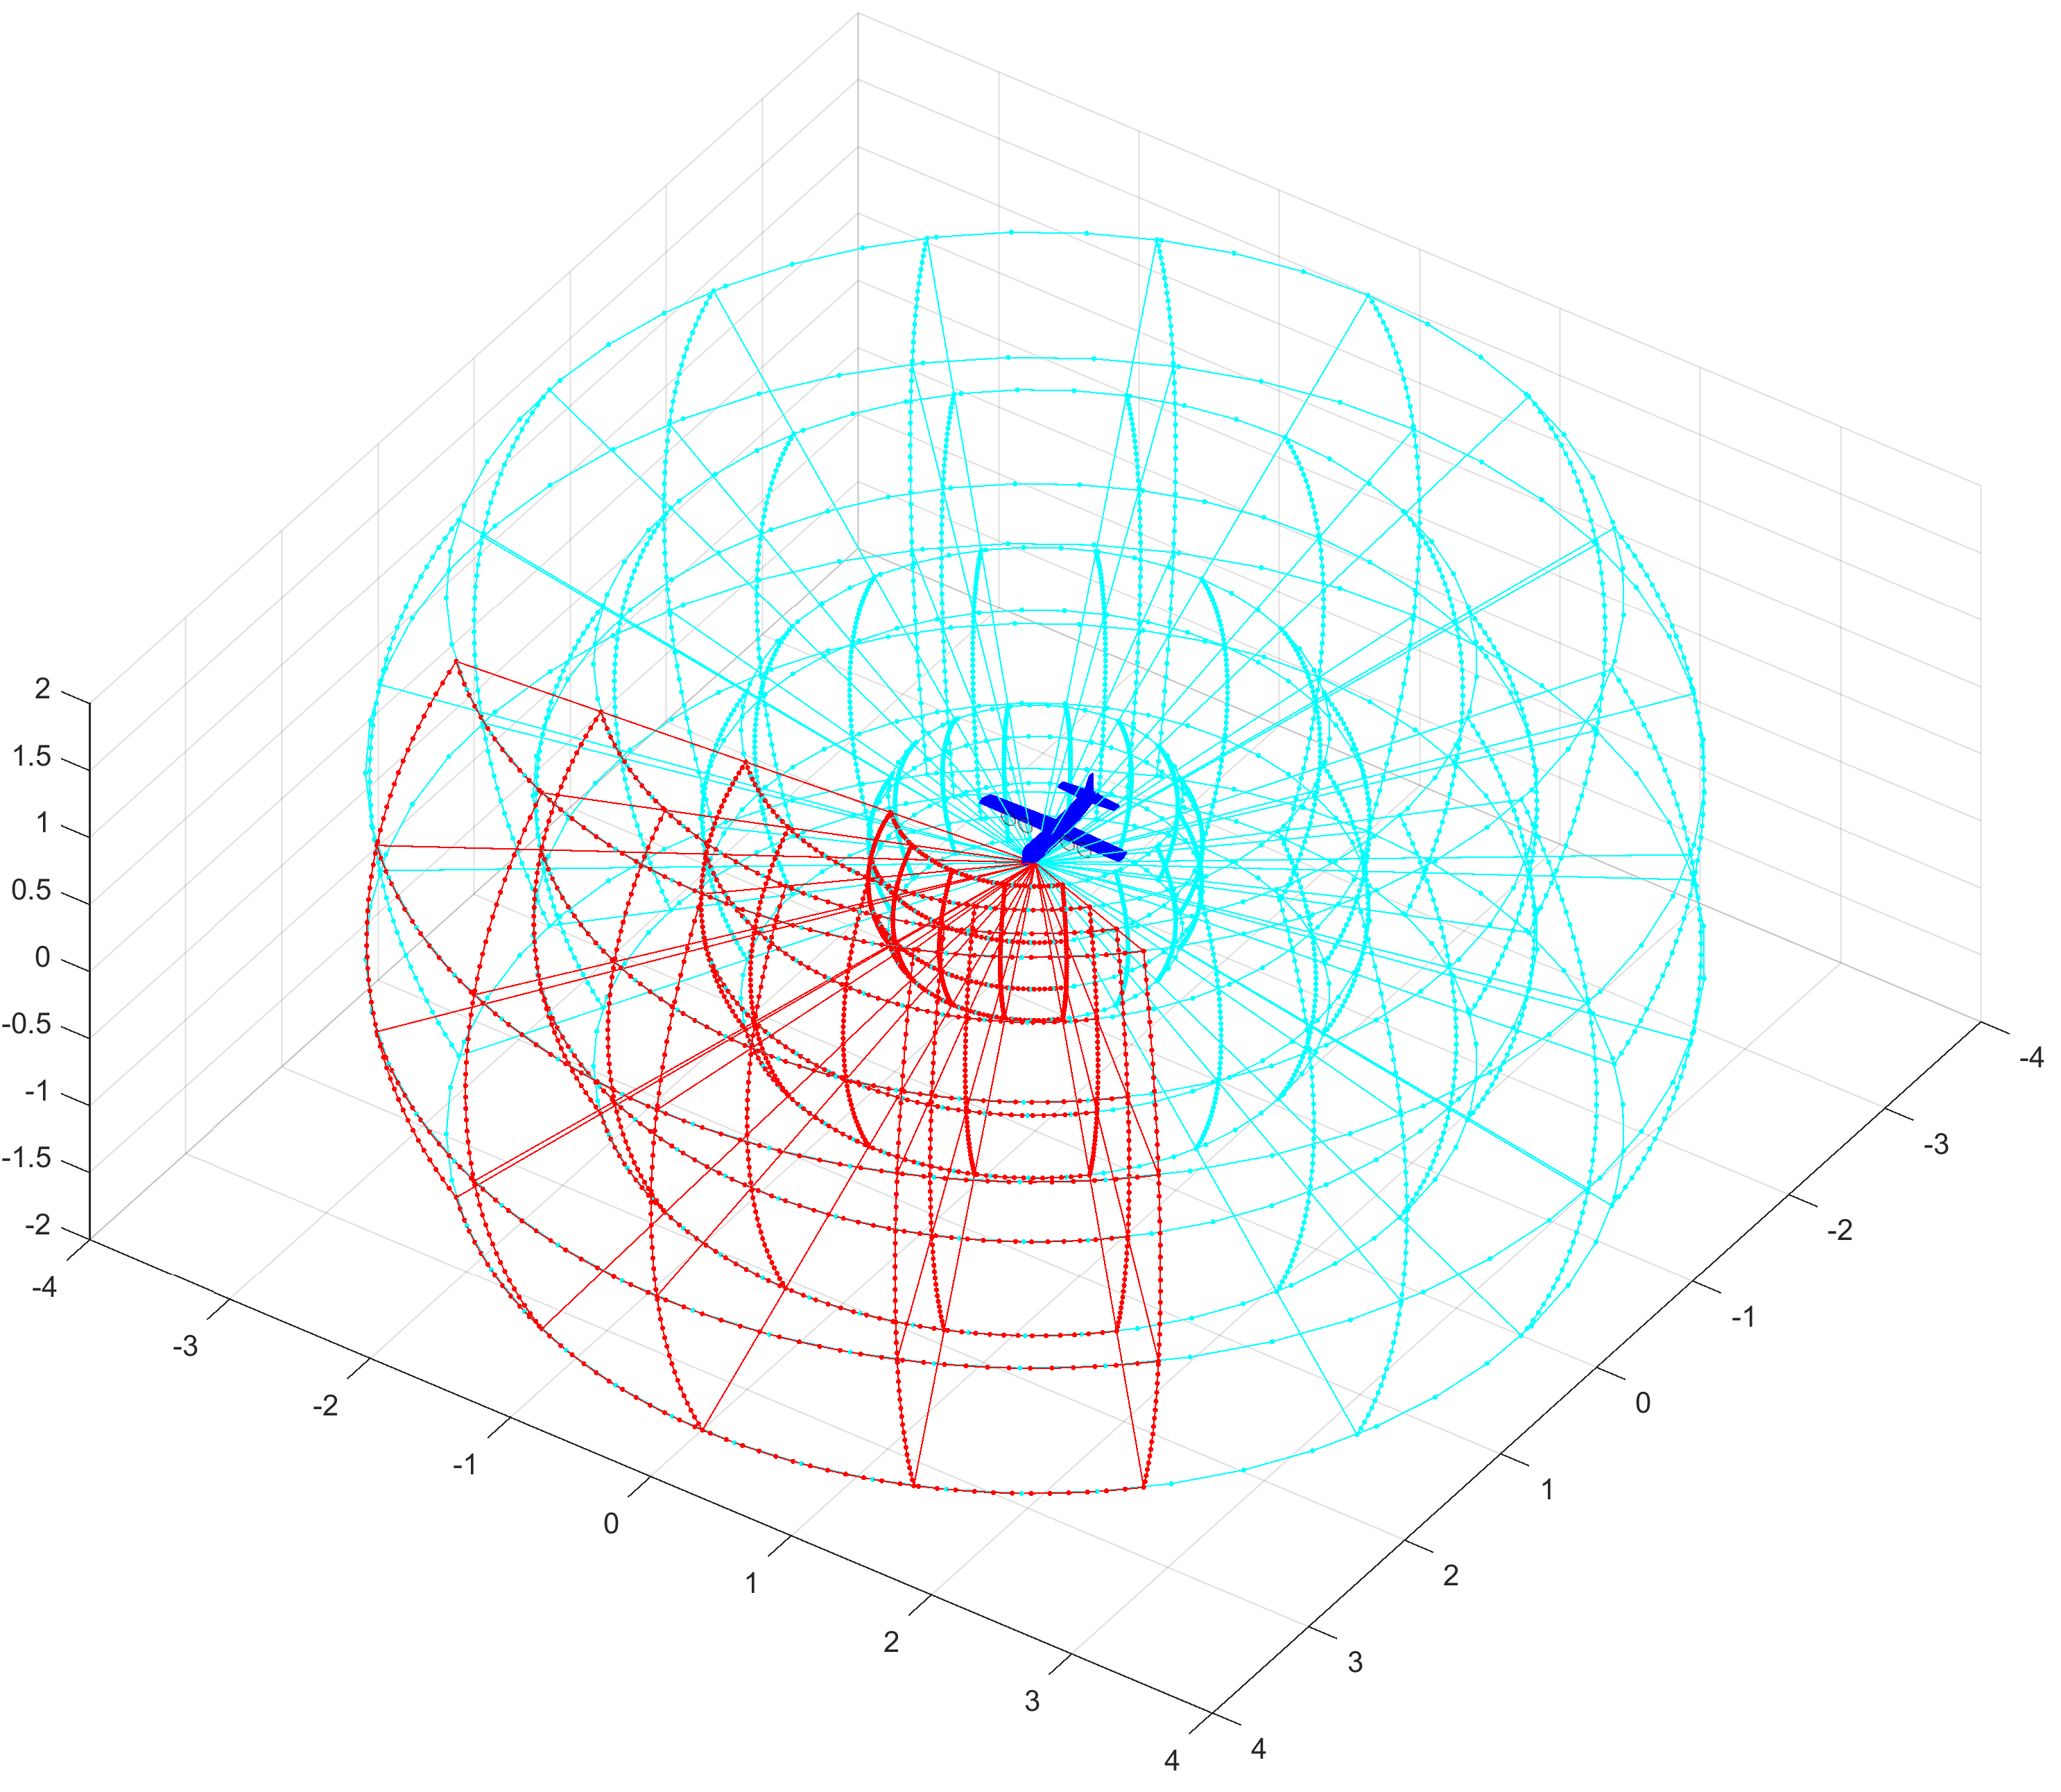
\includegraphics[width=0.80\linewidth]{\FIGDIR/TE046LiDARRasterRange} 
    \caption{Example: The \emph{LiDAR} reading portioning - cells.}
    \label{fig:LidarSpaceSegmentation}
\end{figure}

\paragraph{Avoidance Grid Definition:} The \emph{effective operation space} is going to be portioned into cells. The set of these cells is going to be called \emph{Avoidance Grid}. The idea is to split operational space into cells with even distance, horizontal angle, and vertical angle ranges. 

\begin{definition}{Avoidance Grid}\label{def:AvoidanceGrid} 


\noindent The \emph{effective space portion} (fig. \ref{fig:LidarSpaceSegmentation} red lines) given by a portion of space in UAS local polar coordinate frame, bounded by:
    \begin{enumerate}
        \item \emph{Distance Range} -  in range $distance_{start}$ $<$ $distance_{end}$ $in$ $\R^+$.
        \item \emph{Horizontal Range} - in range by $horizontal^\circ_{start}$ $<$ $horizontal^\circ_{end}$ $\in$ $]-\pi,\pi]$.
        \item \emph{Vertical Range} -in range $vertical^\circ_{start}$ $<$ $vertical^\circ_{end}$ $\in$ $]-\pi,\pi]$.
    \end{enumerate}

\noindent The goal is to separate the \emph{effective operation space} into cells (def. \ref{def:cell}). The idea is to split distance range into multiple distinctive distance ranges with count $layerCount \in \N^+$.  The ranges for \emph{distance layers} are given as follow:
\begin{equation}\label{eq:avoidanceGridCellDistanceRange}
    \begin{aligned}
        layer^i_{start} & = (i-1)\times\frac{distance_{end}-distance_{start}}{layer Count}\\
        layer^i_{end} & = i\times\frac{distance_{end}-distance_{start}}{layer Count}
    \end{aligned};\quad i\in 1\dots layer Count
\end{equation}

\noindent The same separation Layer horizontal/vertical separations separations defined by $horizontal Count \in \N^+$/$vertical Count \in \N^+$:

\begin{equation}\label{eq:avoidanceGridCellHorizontalRange}
    \begin{aligned}
        horizontal^j_{start} & = (j-1)\times\frac{horizontal^\circ_{end}-horizontal^\circ_{start}}{horizontal Count}\\
        horizontal^j_{end} & = j\times\frac{horizontal^\circ_{end}-horizontal^\circ_{start}}{horizontal Count}
    \end{aligned};\quad j\in 1\dots horizontal Count
\end{equation}


\begin{equation}\label{eq:avoidanceGridCellVerticalRange}
    \begin{aligned}
        vertical^k_{start} & = (k-1)\times\frac{vertical^\circ_{end}-vertical^\circ_{start}}{vertical Count}\\
        vertical^k_{end} & = k\times\frac{vertical^\circ_{end}-vertical^\circ_{start}}{vertical Count}
    \end{aligned};\quad k\in 1\dots vertical Count
\end{equation}


\noindent Then $cell_{i,j,k}$ space portion by (def. \ref{def:cell}) has following ranges:
\begin{enumerate}
    \item \emph{Cell Distance Range} (eq. \ref{eq:avoidanceGridCellDistanceRange}) depending on layer index $i$.
    
    \item \emph{Cell Horizontal Angle Range} (eq. \ref{eq:avoidanceGridCellHorizontalRange}) depending on horizontal angle index $j$.
    
    \item \emph{Cell Vertical Angle Range} (eq. \ref{eq:avoidanceGridCellVerticalRange}) depending on vertical index $k$.
\end{enumerate}

\begin{note}
	The example of \emph{Avoidance Grid Cells} is given in (fig. \ref{fig:LidarSpaceSegmentation} red boundary).
\end{note} 

The \emph{Avoidance Grid} is the set of cells:

\begin{equation}\label{eq:avoidanceGridCellSpace}
    Avoidance Grid = \left\{
    					cell_{i,j,k}:
    					\begin{aligned}
    						& i \in 1 \dots layer Count\\
    						& j \in 1 \dots horizontal Count\\
    						& k \in 1 \dots vertical Count
    					\end{aligned} 
                     \right\}
\end{equation}

\begin{note}
	For any distinctive cells $cell_{i,j,k}$, $cell_{m,n,o}$ their \emph{space portion intersection} is empty set:
	\begin{equation}
		\forall cell_{i,j,k}, cell_{m,n,o}:
		\begin{aligned}
		    &cell_{i,j,k}\cap cell_{m,n,o} = \varnothing,
		    i \neq o \lor j \neq n \lor k \neq o
		\end{aligned}
	\end{equation}
\end{note}
\end{definition}

%\paragraph{Trajectory Intersection:} The \emph{trajectory} intersection with \emph{Avoidance Grid} is solved in context of \emph{Reach Set Approximation} (def. \ref{def:ContainedReducedReachSet}). 
%\begin{note}
%    The \emph{trajectory intersection} function does not have an impact on \emph{Reach Set Approximation}, because its done prior the flight.
%\end{note}

\paragraph{Grid Sizing Approach:} The sizing approach used in this work is outlined in (app. \ref{app:gridSizeCalculation}).


\paragraph{Cell in Avoidance Grid Properties:}\noindent For each cell $\vec{p}\in\R^3$ in the there are properties to be checked:

\begin{enumerate}
    \item \emph{Is there visibility to the cell ?} - how good is an observation of the cell by Sensor Field.
    
    \item \emph{Is there threat present ?} - how sure the data fusion is that there is eminent threat in the cell.
    
    \item \emph{Is the cell reachable ?} - if there is any trajectory which can get UAS to that cell without too much threat along the way.
\end{enumerate}

\noindent The answers to these questions are given later in \emph{data fusion procedure}outline (tab. \ref{tab:defuzificationRatings}).
    
	
	%06-06 Reach Set
    	\cleardoublepage
\section{\secState{R}Reach Set Approximation}\label{s:reachSet}

    \noindent\paragraph{Motivation:} \emph{Reach set} is strong tool for \emph{Obstacle Avoidance} because it contains all possible \emph{avoidance maneuvers} in set. The current implementation have following flaws:
    
    \begin{enumerate}
        \item \emph{Realistic approximation} - \emph{nonlinear systems} or \emph{heavily constrained systems} cannot be approximated well by \emph{continuous-time Reach Sets}.
        
        \item \emph{Non Deterministic calculations} - continuous-time \emph{Reach Set} contains  infinite possibilities for \emph{avoidance maneuvers}, the SAA system demands conflict resolution in finite time.
        
        \item \emph{Property binding} - binding related properties seems problematic, because \emph{continuous- time reach sets} does not have unique identifier of maneuver, trajectory nor segment. 
    \end{enumerate}
    
    \paragraph{Proposed Solution Features:} Our Reach set Estimation method will provide following features:
    
    \begin{enumerate}
        \item \emph{System Control Interface} - implemented via \emph{Movement Automaton}, requiring only \emph{discrete command chain} to approximate system behaviour.
        
        \item \emph{Deterministic Calculation} - finite number of elements in \emph{Reach set} will enable \emph{scalable} calculation.
        
        \item \emph{Property binding} - approximation of Reach set as a set of trajectories, each trajectory can be split into finite number of segments. Each element will have unique identifier enabling both-side  property binding.
        
        \item \emph{Behaviour encoding} - some specific behaviour, like horizontal/vertical separation, or maneuver shape can be encoded into \emph{Reach Set}.
    \end{enumerate}
    
    
    \paragraph{Discretization of Reach set:} There is a need for a discrete finite \emph{Reach Set approximation} to enable \emph{Avoidance Strategy Evaluation} in finite time. Replacing \emph{Continuous Control Set} \emph{Inputs(t)} by \emph{Movement Automaton} is feasible:
    
    
    \begin{definition}[Reach set Approximation by Movement Automaton]\label{def:ReachSetApproximationByMovementAutomaton}
        \emph{A trajectory} (def. \ref{def:MovementAutomatonTrajectory}) for system $\dot{state}=f(time,state,input)$ under control of the movement automaton $\mathscr{MA}$ is given as execution of movement buffer (def. \ref{def:MovementBuffer}) with initial state of system $state_0$.  Therefore notation $Trajectory(state_0,buffer)$ is used.
    
        
        \paragraph{The Complete Reach Set} (\ref{eq:reachSetFormalDefintion}) for system with initial state $state_0$ with existing \emph{control strategy} $control(time)\in Controls(time)$. for time  $\tau > time_0$.
        \begin{equation}\label{eq:reachSetFormalDefintion}
            ReachSet(\tau,time_0,state_0) = \bigcup \left\{state(s):control(s)\in Controls(s), s\in (time_0,\tau]\right\} 
        \end{equation}
        
        
        \paragraph{The Reach Set Approximation by Movement Automaton} (\ref{eq:ReachSetDefinitionDiscrete}) of the system under the control of the movement automation $\mathscr{MA}$ consist from the set of trajectories $Trajectory$ $(state_0,$ $Buffer)$, which are executed in constrained time $\tau > time_0$.
        \begin{equation}\label{eq:ReachSetDefinitionDiscrete}
             ReachSet(\tau,time_0,state_0)=\left\{Trajectory(state_0,buffer):
             \begin{gathered}
                \text{duration}(buffer)\\ \le\\ (time_0-\tau)
             \end{gathered}\right\}
        \end{equation}
    \end{definition}
    
    \begin{note}
        \emph{Reach Set Approximation} (def. \ref{def:ReachSetApproximationByMovementAutomaton}) is subset of \emph{Full Reach Set} (def. \ref{def:ReachSetBasic}) in continuous space $\R^n$ it inherits all important properties, like \emph{Invariance} \cite{blanchini1999set}.
        
        \emph{Discretization} of \emph{Reach Set} have been achieved leaving us with \emph{finite count} of \emph{Trajectories}, instead of \emph{Infinite subspace or $\R^N$}
    \end{note}

    \paragraph{Approximated Reach Set Containment:} The \emph{Approximated Reach Set} introduced in (def. \ref{def:ReachSetApproximationByMovementAutomaton}) is constrained only by \emph{future expansion time} $\tau$. UAS makes space assessment in \emph{Avoidance Grid}. There is no point to consider Trajectories outside of \emph{Avoidance Grid}
    
    \begin{definition}[Contained Aproximated Reach Set]\label{def:ContainedReducedReachSet}
        For pair ($state_0$, $AvoidanceGrid_0$) at time $time_0$ and \emph{prediction horizon} $\tau=\infty$ there is \emph{Contained Reduced Reach Set:}
        \begin{equation}\label{eq:containedReachSet}
            ReachSet\left(\begin{gathered}time_0,\\state_0,\\AvoidanceGrid_0\end{gathered}\right) = 
            \left\{
                \begin{gathered}
                Trajectory(\dots) \\\in\\ ReachSet(\ref{eq:ReachSetDefinitionDiscrete})
                \end{gathered}
                :
                \begin{gathered}
                \forall segment \in AvoidanceGrid_0,\\ segment \in Trajectory(\dots)    
                \end{gathered}
            \right\}
        \end{equation}
        
        \paragraph{Properties:} \emph{Container Aproximated Reach Set} contains only trajectories where all segments belongs to \emph{Avoidance Grid}, there are following functions:
        \begin{enumerate}
            \item \emph{Membership function} for any \emph{Trajectory} in \emph{Constrained Reduced Reach set} returns \emph{Ordered Set} of \emph{Passing Cells}. 
            
            \item \emph{Cost function} for any \emph{Trajectory Portion} in \emph{Constrained Reduced Reach Set} return \emph{Cost of Execution}
        \end{enumerate}
        
        \paragraph{Passing cell:} \emph{Cell} of \emph{Avoidance Grid} which has some intersection with {Trajectory}.
    \end{definition}
    
    \begin{note}
        \emph{Contained Reduced Reach Set} (eq. \ref{eq:containedReachSet}) which is contained in \emph{Avoidance Grid} and have an \emph{Membership Function} enable Property transition between Reach set and \emph{Avoidance grid}. 
        
        \emph{Example:} Visibility from cells along \emph{Trajectory} can be gathered to calculate \emph{Trajectory`s} feasibility.
    \end{note}
    
    \paragraph{Reach Set Pruning:} There is a need to implement \emph{Set Difference} between \emph{Reach Set} and 
    \emph{Constraint Set}. Constraint Set cam be \emph{Obstacle Set} from \emph{Known World} (sec. \ref{s:KnownWorld}) and other different constraints.
    
    \paragraph{Reach Set Trajectory Tree:} (\ref{eq:trajectoryTree}) \emph{Any Reach Set} where \emph{Control Strategy Constraint} is implemented as \emph{Movement Automaton}, with defined \emph{Movements} set and for singe initial $state_0$. The \emph{Reach Set} is given as discrete tree with root $Trajectory(state_0,\varnothing)$. 
    
    \begin{equation}\label{eq:trajectoryTree}
        ReachSet(state_0,\dots) = \left\{Trajectory(state_0,buffer):
        \begin{gathered}
            buffer\in Movements^i,\\
            i\in\{1,\dots,k\}
        \end{gathered}\right\}
    \end{equation}
    
    \noindent For each \emph{Trajectory Segment}, there exists \emph{intersection function} which evaluates as true if there exists at least one point in \emph{Segment} which belongs to \emph{Constraint Set}. Formally: 
    \begin{equation}\label{eq:reachsetIntersectionConstraintSet}
        intersection(segment,Set):
        \begin{cases}
            \begin{aligned}\exists &point \in segment,\\ &point \in Set \end{aligned}&: true \\
            Otherwise &: false 
        \end{cases}
    \end{equation}
    
    \begin{definition}[Pruned Reach Set]\label{def:PrunedReachSet} 
        For \emph{Reach set} represented as \emph{Trajectory Tree} (eq. \ref{eq:trajectoryTree}) and some constraint set ($Set$) where exist \emph{intersection function} (eq. \ref{eq:reachsetIntersectionConstraintSet}). The \emph{Pruned Reach set} is given as follows:
        
        \begin{equation}\label{eq:PrunedReachSet}
            Prune(ReachSet,Set) = 
            \left\{
                Trajectory(\dots):
                \begin{gathered} 
                \forall segment \in Trajectory,\\ \neg intersection(segment, Set) 
                \end{gathered}
            \right\}
        \end{equation}
    \end{definition}
    
    
    \begin{note} 
        Pruning(def. \ref{def:PrunedReachSet}) \cite{birmingham1988tree} is applicable multiple times for various \emph{Constraints Set}. 
    
        Example of \emph{Approximated Reach set Calculation} (def. \ref{def:ReachSetApproximationByMovementAutomaton}), \emph{Reach Set Containment} (def. \ref{def:ContainedReducedReachSet}), and, \emph{Pruning} is given in \cite{gomola2017obstacle}.
    \end{note}

    	\subsection{\secState{R}Reach Set Performance Criteria}\label{s:ReachSetPerformanceCriteria}

\paragraph{Motivation:} The need to Make \emph{Reach Set} scalable approach. This may be a problem due the \emph{Expansion rate}. \emph{Reach set} represented as a \emph{Trajectory Tree} (eq. \ref{eq:trajectoryTree}) for Avoidance Grid with $layerCount$ and Movement automaton with $movementCount$, the \emph{Node count} is given as:

\begin{equation}\label{eq:fullReachSetNodeCount}
    1+ \left(\sum_{i\in\{1\dots layerCount\}} (movementCount)^i\right)
\end{equation}

\noindent \emph{This scaling} is not feasible for \emph{Avoidance Grid} with many layers ($< 10$) or \emph{Movement Set} with many movements ($< 9$). There is need for \emph{Reduced Reach set calculation}.

\paragraph{Core Performance Criteria:} The scaling factor (eq. \ref{eq:fullReachSetNodeCount}) shows that there are going to be many trajectories. The main point is that not every trajectory in \emph{Reach Set} are giving us \emph{maneuverability advantage}. Our expectations lies in following \emph{Performance Requirements}:

\begin{enumerate}
    \item \emph{Reach set} must \emph{Cover} maximum of the \emph{possible unique maneuvers} in  \emph{Avoidance Grid}.
    \item \emph{Trajectories} in \emph{Reach Set} should be smoothest possible to prevent cargo damage / UAS wear.
\end{enumerate}

\paragraph{Trajectory footprint:} Discrete space of \emph{Avoidance Grid} is organized in cells. \emph{Cell} is minimal space portion accessible by \emph{property binding}. There is need to know if two trajectories contribution to \emph{Maneuverability} in this environment. 

Each trajectory passes through space in \emph{Avoidance Grid}. If there exists a method to extract unique identifier for each \emph{trajectory passed cells}, we can compare two trajectories \emph{Coverage} in \emph{Avoidance Grid}.


\begin{definition}[Trajectory footprint] \label{def:trajectoryFootprint}
    For \emph{Trajectory} from \emph{Reach set} (def. \ref{def:ContainedReducedReachSet}) defined for \emph{Avoidance Grid} has membership function. \emph{Membership Function} returns \emph{ordered set of passing cells}:
    
    \begin{equation}\label{eq:setOfPassedCells}
        footprint
        \left(\begin{gathered}
            Trajectory,\\
            AvoidanceGrid    
        \end{gathered}\right) 
        = 
        \left\{
            \begin{aligned}
                cell \in& AvoidanceGrid:\\ &isMember(trajectory,cell)
            \end{aligned}
        \right\}
    \end{equation}
    
    \noindent Then we can define equality function for $Trajectory_1$ and $Trajectory_2$, as comparison of their footprints in common \emph{Avoidance Grid} as follow:
    
    \begin{equation}\label{eq:TrajectoryEquality}
        isEqual\left(\begin{gathered}
        Trajectory_1,\\Trajectory_2,\\AvoidanceGrid  
        \end{gathered}\right):
        \begin{cases}
            \left(\begin{gathered}
                footprint(Trajectory_1,\dots)\\
                = \\
                footprint(Trajectory_2,\dots)
            \end{gathered}\right)
            &:true\\
            Otherwise&: false\\
        \end{cases}
    \end{equation}
\end{definition}

\begin{note}
    Depending on \emph{Movement Automaton`s} movement set and \emph{Avoidance Grid} parameters, there can be multiple \emph{trajectories} which are equal.
\end{note}

\paragraph{Coverage set:} Now it is possible to create set of unique \emph{trajectory footprints} due to \emph{footprint function} (eq. \ref{eq:setOfPassedCells}). Similarly there is a possibility to create \emph{Reach set skeleton} containing unique trajectories, by using 
\emph{equality function} (eq. \ref{eq:TrajectoryEquality}).
\emph{Coverage set} is sufficient for now.

\newpage
\begin{definition}[Coverage Set]\label{def:CoverageSet}
    \emph{Coverage set} (\ref{eq:CoverageSet}) is defined for \emph{Avoidance Grid} and \emph{Reach Set} pair as set of unique \emph{Trajectory footprints}:
    
    \begin{equation}\label{eq:CoverageSet}
        CoverageSet\left(\begin{gathered}AvoidanceGrid,\\ReachSet\end{gathered}\right)= \left\{
            footprint\left(\begin{gathered}     
                Trajectory,\\AvoidanceGrid
            \end{gathered}\right):
            \begin{aligned}
                \forall &Trajectory\\ &\in Reach Set
            \end{aligned}\right\}
    \end{equation}
\end{definition}

\paragraph{Coverage set properties:} Trajectory footprint (eq. \ref{eq:setOfPassedCells})is not \emph{bijection}, neither \emph{injection} for $ReachSet \to CoverageSet$. This implies following properties:

\begin{enumerate}
    \item Equal \emph{Reach Sets} in same \emph{Avoidance Grid} have equal \emph{Coverage Sets}.
    
    \item Equal \emph{Coverage Sets} does not imply \emph{Reach Set} equality.
    
    \item For two {Coverage Sets} there is a possibility to compare their member count to create coverage ratio.
\end{enumerate}

The second \emph{Property} gives us a preposition that there is a possibility of \emph{Reach Set Reduction} without loosing 
\emph{Coverage}.  

\begin{definition}[Coverage Ratio]\label{def:coverageRatio}
    \emph{Coverage Ratio} is a ratio of \emph{Coverage Set Member Count} between two \emph{Reach Sets}. Reach set with \emph{lesser count of unique Trajectories} is considered as \emph{Reduced Reach Set}.  Reach set with \emph{greater Count of unique Trajectories} is considered as \emph{Reference Reach Set}.
    
    \begin{equation}\label{eq:CoverageRatio} 
        \begin{gathered}
            referenceCoverage=|CoverageSet(ReferenceReachSet,AvoidanceGrid)|\\
            reducedCoverage=|CoverageSet(ReducedReachSet,AvoidanceGrid)|\\
            CoverageRatio = \frac{reducedCoverage}{referenceCoverage}\in[0,1]
        \end{gathered}
    \end{equation}
\end{definition}

\begin{note}
    \emph{Reference Reach Set} is usually \emph{Full Reach Set} containing all possible trajectories in space contained by \emph{Avoidance Grid}. In case \emph{Full Reach Set} cannot be computed, Avoidance Grid is too large, most complex \emph{Reach Set} is used as \emph{Reference Reach Set}.
\end{note}

\paragraph{Trajectory smoothness:} Trajectory other than straight line have some changes in \emph{UAS} heading. 

The goal is to minimize \emph{Maneuvering} of UAS, because:
\begin{enumerate}
    \item \emph{Every Heading Change} needs to be reported to \emph{UTM}.
    \item \emph{Sharp Maneuvering} can damage cargo/wear UAS.
    \item \emph{Often course changes} makes \emph{Intruder prediction} harder for other Civil General Aviation.
\end{enumerate}

\noindent For this purpose \emph{Smoothness Metric} needs to be applied for \emph{Reach Set} or \emph{Trajectory}.  In case of \emph{Movement Automaton Control} two distinguish \emph{Movement Sets} can be introduced:\emph{Smooth} nad \emph{Chaotic} movements set with following properties:

\begin{equation}\label{eq:ChaoticSmoothMovementSetDefinition}
    \begin{gathered}
        MovementSet=SmoothMovements\cup ChaoticMovements\\
        SmoothMovements\cap ChaoticMovements = \varnothing\\
        |SmoothMovements| > 0, \quad |ChaoticMovements|>0
    \end{gathered}
\end{equation}

Then \emph{Smoothnes clasificator} for $Trajectory(initialState,buffer)$ can be defined as $isSmooth$ and \emph{Smooth Movement Counter} function as $smoothCount$ like follow:

\begin{equation}\label{eq:SmoothnesClasificatorCounter}
    \begin{gathered}
        isSmooth(movement)=
        \begin{cases}
            movement \in SmoothMovements &:1\\
            movement \in ChaoticMovements &:0
        \end{cases}\\
        smoothCount(Trajectory(\dots,buffer))= 
        \begin{aligned}
            \sum isS&mooth(movement),\\& \forall movement \in Buffer
        \end{aligned}
    \end{gathered}
\end{equation}

\begin{definition}[Smoothness Rating for Trajectory]\label{def:SmoothnessRatingForTrajectory} 
    \emph{Smoothness} for trajectory generated by \emph{Movement Automaton} for some \emph{Initial State} with some \emph{Movement Buffer}, under assumption of \emph{Smooth and Chaotic Movement Set} split (eq. \ref{eq:ChaoticSmoothMovementSetDefinition}), with existing \emph{classification} and \emph{counter} functionals (eq. \ref{eq:SmoothnesClasificatorCounter}) is given as follows:

    \begin{equation}
        Smoothness(Trajectory(\dots,buffer)) = \frac{isSmooth(Trajectory)}{movementCount(Trajectory)} \in [0,1] 
    \end{equation}
    
    \noindent For \emph{Trajectory} with $buffer=\varnothing$ \emph{Smoothness} is given as 1.
\end{definition}

    	\subsection{\secState{R}Constrained Trajectory Expansion}\label{s:constrainedTrajectoryExpansion}

\paragraph{Motivation:} \emph{Purpose} of \emph{Navigation} is to move forward to \emph{Goal Waypoint} in \emph{Mission}. \emph{Structure} of \emph{Avoidance Grid} is designed to enable \emph{forward} and \emph{turning} maneuvers. The \emph{Avoidance Grid} is organized in \emph{Layers} characteristic by same distance from \emph{Avoidance Grid Origin}. 

Survey of motion planning algorithm was given in \cite{goerzen2009survey}. The ideal candidate for propagation algorithm is \emph{Wave-front} algorithm propagating \emph{Trajectory tree} through Layers. Due the \emph{Avoidance Grid} onion like layers, there is possibility to implement turn maneuver through layers iterative and effectively .

\begin{figure}[H]
    \centering
    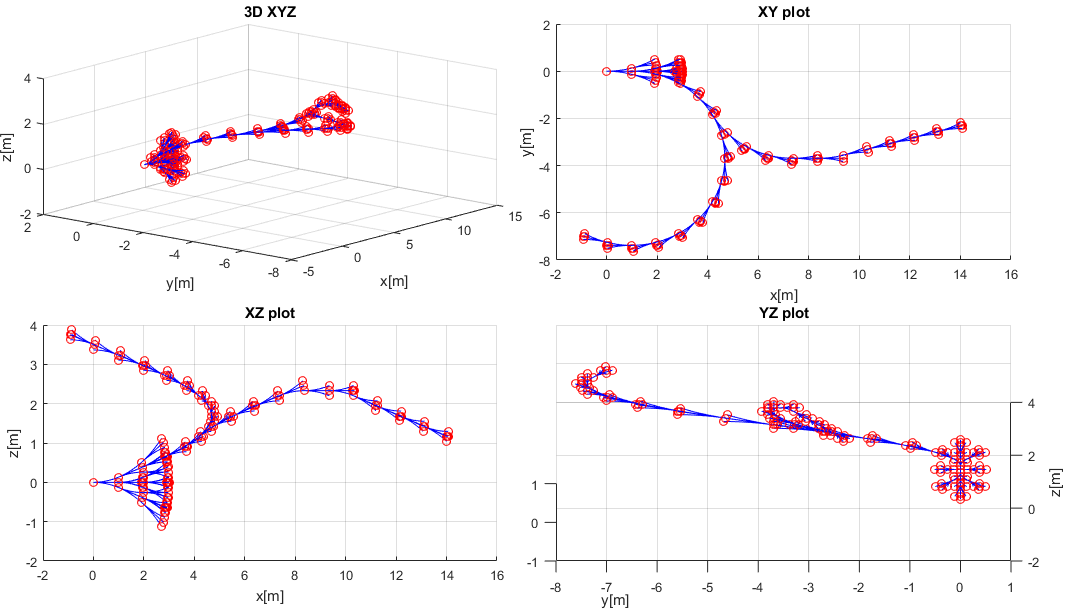
\includegraphics[width=0.9\linewidth]{\FIGDIR/RS001RapidExplorationTreeExampleShrink} 
    \caption{\emph{Rapid Exploration tree as result of \emph{Constrained trajectory expansion}}.}
    \label{fig:rapidExplorationTrajectoryTree}
\end{figure}

\paragraph{Rapid Exploration Tree} (fig. \ref{fig:rapidExplorationTrajectoryTree}) was selected, because it enables \emph{Movement Automaton Utilization} and \emph{Property Binding}. Similar approach was used for space exploration \cite{plaisant2002spacetree}. 

\paragraph{The example} (fig. \ref{fig:rapidExplorationTrajectoryTree}) shows a \emph{Rapid Exploration Tree} in \emph{Free Space} containing \emph{Waypoint Navigation Path} and \emph{Turn Away Path}. Both paths are starting in same \emph{Root Node} (red circle) which was expanded with simple \emph{Movement Automaton} (bunch of nodes originating from one node are showing way of expansion). The connection (blue line) between two nodes (red circles) represents \emph{Trajectory portion} for \emph{Executed Movement}.

\paragraph{Rapid Exploration Tree Node} will contain following information:
\begin{enumerate}
    \item \emph{Initial state} - root entry point, used in state evolution calculation.
    \item \emph{Trajectory (state evolution)} - trajectory passing through \emph{state space} in local coordinate frame of \emph{Avoidance Grid}.
    \item \emph{Buffer} (applied movements) - ordered list of \emph{executed movements} applied on \emph{initial state} to obtain \emph{state evolution}.
    \item \emph{Cost} - calculated for \emph{state evolution} based on \emph{predefined cost function}. 
    \item \emph{Footprint} - ordered set of \emph{passing cells} in \emph{Avoidance Grid}.
    \item \emph{Parent Node Reference} - tree reference for parent node, not in case of \emph{root node}.
    \item \emph{Other Bounded Properties} - value list of other properties, depending on \emph{Expansion Constraints} and \emph{Reachability} evaluation algorithm.
\end{enumerate}

\paragraph{Wave-front propagation of Rapid Exploration Tree} is given in (alg. \ref{alg:Wavefront Propagation}). 

The \emph{Avoidance Grid} have UAS with \emph{position $\in$ Initial State} at the \emph{origin}. The \emph{Grid Layer} is a column ordered set of cells with same \emph{Mean distance} from origin. \emph{Grid Layers} are indexed from origin starting with $1$, there is maximum of \emph{i $\ge$ 1} layers.

\paragraph{Step: Initialization} contains base structure preparation like follows:
\begin{enumerate}
    \item \emph{Avoidance Grid} - Space containing \emph{Reach set} (def. \ref{def:ContainedReducedReachSet}).
    \item \emph{Movement Automaton} - Used as \emph{Predictor}, consuming \emph{buffer} containing \emph{Movements} to generate $Trajectory(initialState,buffer)$.
    
    \item \emph{Reach Set} -  tree consisting from \emph{Wave-frontNodes} representing the end point of $Trajectory(initialState,buffer)$ where each \emph{Edge} represents \emph{one Movement application}. The root is set as node containing \emph{Initial State}.
\end{enumerate}

\noindent Function \emph{initializeReachSet(root,stack,grid,automaton)} will take the root and enforces \emph{full wavefornt propagation} to \emph{First Layer}.


\paragraph{Step: Wave-front Propagation} is forced propagation of trajectories from layer $i$ to layer $i+1$. The process goes as follows:
\begin{enumerate}
    \item \emph{Selection of Feasible candidates} - function \emph{[candidates,leftovers] = ExpansionConstraints.select(stack)} for working layer, row and cell selects \emph{feasible trajectory nodes} ordered by \emph{Cost function}. The \emph{Example of Cost Function} can be \emph{Trajectory Smoothness} (def. \ref{def:SmoothnessRatingForTrajectory}).
    
    \item \emph{Expansion of Candidates} - for each \emph{candidate} function \emph{candidate.expandNode (automaton)} is invoked. This function will expand \emph{Candidate Node structure} by appending \emph{Full Trajectory Tree Evolution} until each \emph{Leaf Trajectory} reaches \emph{Next Layer}. Simply put \emph{Par rent Node} \emph{Node(initialState, buffer, cost, footprint )} buffer is appended by movements until the next layer is reached.
    
    \item \emph{Leftovers purge} - function \emph{reachSet.purge(leftovers)} removes unexpanded \emph{Nodes} leading to cell, effectively  removing trajectories which does not  lead to \emph{next layer}.
    
    \item \emph{Append Reach Set} - function \emph{reachSet.append(leafs)} puts newly created \emph{Nodes (Trees)} into \emph{Reach Set} structure. The \emph{Wave-front Propagation} for one cell is finished.
\end{enumerate}

\paragraph{Step: After Layer Propagation Purge} is covered by function \emph{reachSet.purgeSame- Footprint()} which takes trajectories with same footprint and keeps some of them based on \emph{Selection criteria}, more in (sec. \ref{s:chaoticReachSet}, \ref{s:harmonicReachSet}). \emph{Pruning methods} over \emph{Large Decision Trees} are \emph{fast} and \emph{viable} \cite{mingers1989empirical}.

\begin{note}
    \emph{Reach Set} is usually computed \emph{Prior the Flight} for \emph{some Initial State} in \emph{Local Coordinate Frame} in \emph{right had coordinate frame} with $X^+$ used as \emph{main axis}.
\end{note}


\begin{algorithm}[H]
    \SetKwInOut{Input}{Input}\SetKwInOut{Output}{Output}
    \Input{Node(initialState,buffer=$\varnothing$,cost=0,footprint=$\varnothing$),
           AvoidanceGrid, ExpansionConstraints, MovementAutomaton(movementSet)
    }
    \Output{ReachSet(AvoidanceGrid)}
    \BlankLine
    \# Initialization Sequence\;
    grid=AvoidanceGrid, automaton=MovementAutomaton, root = Node\;
    reachSet = initializeReachSet(root,stack,grid,automaton)\;
    \BlankLine
    \# Main Expansion through, layers (i), rows (j), cells(k)\;
    \For{layer($1\dots i$) \emph{in} grid}{
        \For{row($1\dots j$ \emph{in} layer)}{
            \For{cell($1 \dots k$) \emph{in} row}{
                \BlankLine
                \# apply selection criteria \;
                [candidates,leftovers] = ExpansionConstraints.select(stack)\;
                \BlankLine
                \# collect expansions \;
                leafs = []\;
                \For{candidate \emph{in} Candidates}{
                    leafs= [leafs, candidate.expandNode(automaton)];
                }
                reachSet.purge(leftovers)\;
                reachSet.append(leafs)\;
            }
        }
        reachSet.purgeSameFootprint()\;
    }
    \caption{\emph{Wave-front propagation} of \emph{Rapid Exploration Tree} to form \emph{Reach Set}.}
    \label{alg:Wavefront Propagation}
\end{algorithm}






    	%\subsection{(W) Avoidance Grid scaling}\label{s:avoidanceGridScaling}
    \begin{itemize}
        \item Supplement to avoidance grid scaling, based on movement set properties 
        \item Formula for Theta and Varphi parameters adjustment
    \end{itemize}
    

    	
\subsection{(R) Chaotic Reach set}\label{s:chaoticReachSet}

\paragraph{Motivation:} Design of calculation method for \emph{Reach Set Approximation} guarantying high \emph{Maneuverability}.

\paragraph{Background:}There is \emph{Coverage Ratio} property of \emph{Reach Set} (def. \ref{def:coverageRatio}). It has been shown that creating \emph{Reach Set} via \emph{greedy approach} is not feasible due the \emph{Scaling Factor}.  \emph{Contracted Expansion} (sec. \ref{s:constrainedTrajectoryExpansion}) is enabling to apply selection criteria while building \emph{Reach Set} in given \emph{Cell}. 

The \emph{Cell} $cell_{i,j,k}$ has a center and walls from UAS viewpoint: front wall , back wall (for $layer > 1$), top wall, left wall, right wall, bottom wall. It is expected that trajectory leading close to one cell walls will continue to different cell, increasing chance to obtain more \emph{Unique Footprints}. 

\paragraph{Expansion Constraint Function Implementation} (alg. \ref{alg:ExpansionConstraintFunctionForChaoticReachSet}) is based on simple principle: \emph{Select candidate Nodes which are  closest to outer walls of Cell, with unique footprint}.

\paragraph{Tuning Parameters}: \emph{Proximity to Cell outer wall} gives good chances to break into other rows or columns in \emph{Avoidance Grid}. \emph{Unique footprint} guarantees future \emph{Unique Footprint} after appending Trajectory by \emph{Movement application}. 
\begin{enumerate}
    \item \emph{Considered Footprint Length} - how much last cells in footprint should be considered in unique path track, minimal value 1, default value 3, maximal value $\infty$. If you want to generate non redundant trajectories use $\infty$, it will consider full footprint.
    
    \item \emph{Spread Limit} - upper limit of candidates which are going to be select for further expansion, minimal value 1, default value \emph{Count of unique Moves in Movement set}, maximal value $\infty$. If more than default values is selected the algorithm will generate \emph{redundant trajectories}. If less is selected then some trajectories are omitted and \emph{Coverage Rate} decreases sharply. 
\end{enumerate}


\paragraph{Step: Initialization} initialization of \emph{candidate} array (return value), \emph{leftovers} array (return Value). Node array \emph{passing} is populated with \emph{Nodes} which represents \emph{end node of Trajectory} and the tip of \emph{trajectory is constrained in \emph{cell}$_{i,j,k}$}.

\paragraph{Step: Evaluate best trajectories with unique Footprints} following steps are executed:
\begin{enumerate}
    \item \emph{Best Performance Map} is created with \emph{footprint} as key set element to ensure footprint uniqueness.
    \item \emph{Wall distance} for \emph{test node} is calculated as a closest trajectory portion distance to \emph{top, bottom, left, right} wall of cell $cell_{i,j,k}$
    \item \emph{Footprint} for \emph{test node} is created with maximal length given by \emph{Footprint Length} tuning parameter.
    \item \emph{Existence and Performance Test} is executed to ensure that best performing node is selected. If there is not key entry in the \emph{Best Performance Map}, then new entry for \emph{Test Node} is created. If there is key entry, the performance of \emph{Old Node} and \emph{Test Node} is compared and better is stored.
\end{enumerate}

\paragraph{Step: Select candidates} is executed on \emph{Best Performance Map} records using  \emph{Wall distance} as pivot parameter, ordering by closest proximity and limited by \emph{Search Limit} tuning parameter. The \emph{Leftovers} are difference set between \emph{Passing Nodes} and \emph{Candidate Nodes}. 

\begin{algorithm}[H]
    \SetKwInOut{Input}{Input}\SetKwInOut{Output}{Output}\SetKwInOut{TuningParameters}{Tuning Parameters}
    \Input{Node[] stack, Cell cell$_{i,j,k}$}
    \TuningParameters{int$^+$ footprintLength, int$^+$ spreadLimit}
    \Output{Node[] candidates, Node[] leftovers}
    
    \BlankLine
    \# Initialize structures\;
    Node[] candidates = [], Node[] leftovers=[]\;
    Node[] passing = cell$_{i,j,k}$.getFinishingTrajectories(stack)\;
    
    \BlankLine
    \# Select best performing trajectories with unique footprint\;
    Map$<$Footprint,Node$>$  bestPerformanceMap\;
    \For{Node test $\in$ passing}{
        wallDistance= test.minimalDistanceToWall(cell$_{i,j,k}$)]\;
        footPrint = test.getFootprint(lastCells = footprintLength)\;
        \eIf{bestPerformanceMap.contains(footPrint)}{
            old = bestPerformanceMap.getByKey(footprint)\;
            oldPerformance= old.minimalDistanceToWall(cell$_{i,j,k}$)\;
            \If{oldPerformance $>$ wallDistance}{
                bestPerformanceMap.setByKey(footprint,test)\;         
            }
        }{
            bestPerformanceMap.setByKey(footprint,test)\;
        }
    }
    
    \BlankLine
    \# Select best performing nodes up to \emph{spreadLimit} count\;
    candidates = bestPerformanceMap.select(count = spreadLimit).orderBy('wallDistance','Ascending')\;
    leftovers = passing - candidates\;
    \Return{[candidates,leftovers]}
    
    
    \caption{Expansion Constraint function for \emph{Chaotic Reach Set Approximation}}
    \label{alg:ExpansionConstraintFunctionForChaoticReachSet}
\end{algorithm}

\paragraph{Example:} for \emph{Avoidance Grid} with \emph{Distance 10 m}, \emph{Layer count 10}, \emph{Horizontal range $[-45^\circ,+45^\circ]$}, \emph{Horizontal Cell Count 7}, \emph{Vertical range $[-30^\circ,+30^\circ]$}, and \emph{Vertical Cell Count 5}. Is given in (fig. \ref{fig:chaoticReachSetApproximation}). The UAS is at \emph{Back-side} of \emph{Figure} (initial state is at all \emph{Trajectory Origins}). The \emph{black dashed line} marks \emph{Avoidance Grid} space boundary. Each trajectory has its own color and ends at \emph{Front-side} of \emph{Avoidance Grid Boundary}.


\begin{figure}[H]
    \centering
    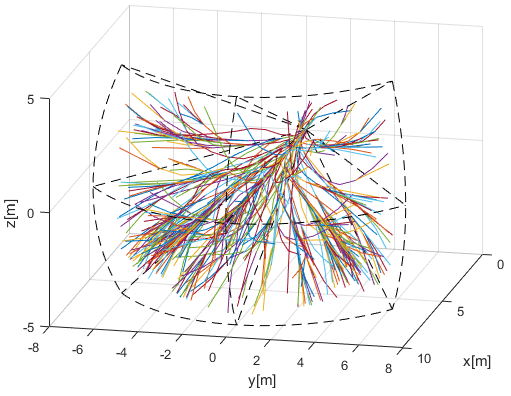
\includegraphics[width=0.7\linewidth]{\FIGDIR/RS002ChaoticReachSetEstimationMethod} 
    \caption{\emph{Chaotic \emph{reach set} approximation}.}
    \label{fig:chaoticReachSetApproximation}
\end{figure}

\paragraph{Pros and Cons:} It can be seen from example (fig. \ref{fig:chaoticReachSetApproximation}) that \emph{Chaotic Reach Set Approximation Method} (alg. \ref{alg:ExpansionConstraintFunctionForChaoticReachSet}) generates a lot of \emph{turning} and \emph{shaky} \emph{trajectories}. 

\emph{High Coverage Ratio} ($\sim 0.9$) is provided, while keeping \emph{medium node count}. The calculation complexity scales linearly with grid size. The \emph{upper limit of trajectories} is given as follow:

\begin{multline}
    countTrajectories(ReachSet) \le layerCellCount \times spreadLimit\\ \times size(Movements)
\end{multline}

\noindent The \emph{upper limit of nodes} is given as follow:
    
\begin{multline}
    countNodes(ReachSet) \le layerCount \times  layerCellCount  \\
    \times size(Movements) \times spreadLimit  
\end{multline}

\noindent\emph{Absence} of \emph{Smooth Trajectories} disqualifies \emph{Chaotic Reach Set Approximation} to be used for \emph{Navigation}. This type of reach set is feasible for \emph{Avoidance}, because it contains variety of maneuvers.


\subsection{(R) Harmonic Reach set}\label{s:harmonicReachSet}

\paragraph{Motivation:} Imagine having an \emph{Avoidance Grid} like (fig. \ref{fig:LidarSpaceSegmentation}). There is a need of \emph{Reach Set Approximation} which will have \emph{Smooth Trajectories} (def. \ref{def:SmoothnessRatingForTrajectory}) going nearby $cell$ centers.

\paragraph{Background:} The \emph{Smoothness Rating for Trajectory} (def. \ref{def:SmoothnessRatingForTrajectory}) uses two distinct sets \emph{Smooth Movements} and \emph{Chaotic Movements} (eq. \ref{eq:ChaoticSmoothMovementSetDefinition}) which are defined for our \emph{Movement Automaton}  (sec. \ref{s:modelMAImplementation}) like follow:

\begin{equation}
    \begin{aligned}
    Smooth Movements &= \{Straight\} \\
    Chaotic Movements &= Movements - Smooth Movements\\
    \end{aligned}
\end{equation}

\emph{Smooth Movements} contains only \emph{Straight} movement, because others are considered as extreme turning movements. \emph{Smooth Movements} should contain only direct flight movements or slight heading correction. \emph{Chaotic Movements} set is supplement of \emph{Movement Automaton`s Movement Set}. 

The \emph{Avoidance Grid} (fig. \ref{fig:LidarSpaceSegmentation}) cell centers for fixed indexes $j_{fix}$, $k_{fix}$ are linearly aligned with \emph{initial state}. That means that  cell centers of cells $cell_{1,j_{fix},k_{fix}},\dots, cell_{i,j_{fix},k_{fix}}$, where $i$ is count of \emph{layers} lies on one line.  If the trajectory can achieve \emph{cell center} on some \emph{layer} only minor trajectory corrections are required to stay on given line. This type of trajectory gives us following advantages:
\begin{enumerate}
    \item\emph{Minimal steering at beginning} - the minimal steering is advantageous in \emph{Controlled Airspace} because is diminishing the amount of communication to \emph{UTM Service}.
    
    \item\emph{Additional safe space in Linear segment} - once the \emph{center of cell} is reached, \emph{Trajectory} sticks to line between cell centers. Each point on this line has \emph{maximal distance} to outer walls of cell. This gives us extra space given as minimum of distance between \emph{UAS position} and \emph{Outer cell walls}.
\end{enumerate}

\paragraph{Expansion Constraint Function Implementation} (alg. \ref{alg:ExpansionConstraintFunctionForHarmonicReachSet}) is based on simple principle: \emph{Select candidate Nodes  which are closest to Cell center, with unique footprint}.

\begin{note}
    \emph{Cell center} can be closely reached by \emph{smooth movement} from previous cell or \emph{chaotic movement} from neighbouring cell from current or previous layer. These trajectories are usually equivalent in \emph{Smoothness}.
\end{note}

\paragraph{Tuning Parameter:} \emph{Proximity to Cell Center} gives a good chance to keep trajectory smooth or \emph{smooth after one correction maneuver}. It has been mentioned that \emph{Cell Center} can be reached by various trajectories. In this method full footprint length is always considered, therefore only one tuning parameter can be offered:
\begin{enumerate}
    \item \emph{Spread Limit} - upper limit of candidates which are going to be selected for further expansion, minimal value 1, default value \emph{Count of unique Moves in Movement set}, maximal value $\infty$. If maximal value $\infty$ is selected, algorithm will generate skeleton of \emph{Reach Set} with full Coverage and with the smoothest \emph{Trajectories}.
\end{enumerate}

\paragraph{Step: Initialization} sets candidate \emph{Nodes} as empty set, leftover \emph{Nodes} as empty set. and selects all \emph{Nodes} from \emph{Stack} which represents  \emph{Finishing Trajectories} in working cell $cell_{i,j,k}$.

\paragraph{Step: Evaluate smoothest trajectories with unique Footprints} is implemented as \emph{multi-criteria filtration}. 

\emph{First criterion} is \emph{distance to Cell Center} which is penalized by trajectory \emph{smoothness rate} implemented in method \emph{Node.getPerformance(Cell $cell_{i,j,k}$)} defined as follow.

\begin{equation}
    getPerformance(Node,Cell) = \frac{distance(Node.Trajectory,Cell.Center)}{SmoothnessRate(Node.Trajectory)}
\end{equation}

\noindent Distance of \emph{Trajectory} is \emph{enumerator}, because its considered as \emph{base value} and is defined in interval $[0,maximalWallDistance]$. The \emph{Smoothness Rate} is in denominator, because it is a penalization coefficient defined in interval $[0,1]$. 

\emph{Second criterion} is \emph{trajectory uniqueness} This is provided by \emph{Best Performance Map}, where best performing \emph{Node} belongs to one unique \emph{trajectory footprint}. The implementation is identical to \emph{chaotic reach set expansion} (alg. \ref{alg:ExpansionConstraintFunctionForChaoticReachSet}).

\paragraph{Step: Select candidates} is executed  on \emph{Best Performance Map} records using \emph{Penalized Cell Center Distance} as pivot parameter, ordered in ascending order and limited by \emph{Spread Limit} tuning parameter. The \emph{Leftovers} are difference set between \emph{Passing Nodes} and \emph{Candidate Nodes}.

\begin{algorithm}[H]
\SetKwInOut{Input}{Input}\SetKwInOut{Output}{Output}\SetKwInOut{TuningParameters}{Tuning Parameters}
    \Input{Node[] stack, Cell cell$_{i,j,k}$}
    \TuningParameters{int$^+$ spreadLimit}
    \Output{Node[] candidates, Node[] leftovers}
    
    \BlankLine
    \# Initialize structures\;
    Node[] candidates = [], Node[] leftovers=[]\;
    Node[] passing = cell$_{i,j,k}$.getFinishingTrajectories(stack)\;
    
    \BlankLine
    \# Select unique smoothest trajectories\;
    Map$<$Buffer,Node$>$  bestPerformanceMap\;
    \For{Node test $\in$ passing}{
        centerDistance= test.getPerformance(cell$_{i,j,k}$)]\;
        footPrint = test.getFootprint()\;
        \eIf{bestPerformanceMap.contains(footPrint)}{
            old = bestPerformanceMap.getByKey(footprint)\;
            oldPerformance= old.getPerformance(cell$_{i,j,k}$)\;
            \If{oldPerformance $>$ centerDistance}{
                bestPerformanceMap.setByKey(footprint,test)\;         
            }
        }{
            bestPerformanceMap.setByKey(footprint,test)\;
        }
    }
    
    \BlankLine
    \# Select best performing nodes up to \emph{spreadLimit} count\;
    candidates = bestPerformanceMap.select(count = spreadLimit).orderBy('cellCenterDistance','Ascending')\;
    leftovers = passing - candidates\;
    \Return{[candidates,leftovers]}
    
    
    \caption{Expansion Constraint function for \emph{Harmonic Reach Set Approximation}}
    \label{alg:ExpansionConstraintFunctionForHarmonicReachSet}    
\end{algorithm}


\paragraph{Example:} for \emph{Avoidance Grid} with \emph{Distance 10 m}, \emph{Layer count 10}, \emph{Horizontal range $[-45^\circ,+45^\circ]$}, \emph{Horizontal Cell Count 7}, \emph{Vertical range $[-30^\circ,+30^\circ]$}, and \emph{Vertical Cell Count 5}. Is given in (fig. \ref{fig:harmonicReachSetApproximation}). The UAS is at \emph{Back-side} of \emph{Figure} (initial state is at all \emph{Trajectory Origins}). The \emph{black dashed line} marks \emph{Avoidance Grid} space boundary. Each trajectory has its own color and ends at \emph{Front-side} of \emph{Avoidance Grid Boundary}. The \emph{Spread Limit} in this case was set to $9$ which is \emph{Size of the Movement Set}.

\begin{note}
    Please note \emph{Trajectories} are organized in bundles going around \emph{Cell Centers smoothly}. Most of the steering maneuvers are executed at the \emph{beginning} of \emph{Avoidance Grid}.
\end{note}

\begin{figure}[H]
    \centering
    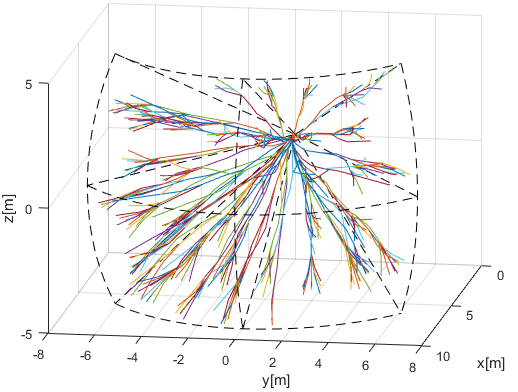
\includegraphics[width=0.7\linewidth]{\FIGDIR/RS003HarmonicReachSetEstimationMethod} 
    \caption{\emph{Harmonic \emph{reach set} approximation}.}
    \label{fig:harmonicReachSetApproximation}
\end{figure}

\paragraph{Pros and Cons:} It can bee seen from example (fig. \ref{fig:harmonicReachSetApproximation}) that \emph{Harmonic Reach Set Approximation Method} (alg. \ref{alg:ExpansionConstraintFunctionForHarmonicReachSet}) generates \emph{smooth evenly spread trajectories}.
    
High smoothness ratio ($\ge 0.9$) is provided, while keeping low node count for UAS systems. The calculation complexity scales linearly with grid size. The upper limit of trajectories is given as follow:

\begin{multline}
    countTrajectories(ReachSet) \le layerCellCount \times spreadLimit \\\times size(Movements)
\end{multline}

\noindent The \emph{upper limit of nodes} is given as follow:

\begin{equation}
    countNodes(ReachSet) \le layerCount \times layerCellCount \times spreadLimit
\end{equation}

\noindent Absence of \emph{High Coverage Ratio} disqualifies \emph{Harmonic Reach Set Approximation} to be used for \emph{Emergency Avoidance}. This type of \emph{Reach Set} is feasible for \emph{Open Space Navigation} or \emph{Controlled Airspace Navigation}. Its low turning rate in contained \emph{Trajectories} are desired for such tasks. 



\subsection{(R) Combined Reach set}\label{s:combinedReachSet}
\paragraph{Motivation:} Harmonic reach set (sec. \ref{s:harmonicReachSet}) is \emph{efficient} for \emph{Navigation in \emph{Controlled Airspace}}. Chaotic reach set (sec. \ref{s:chaoticReachSet}) is good for \emph{Emergency avoidance}. The need to differentiation between \emph{Navigation} and \emph{Emergency Avoidance} mode is necessary in \emph{Controlled Airspace}. but not in \emph{Non-controlled Airspace}. The combination of \emph{Harmonic} and \emph{Chaotic} reach sets is obvious solution. 

\emph{Automatic mode switch} can be provided by combination of \emph{Navigation Reach Set} and \emph{Avoidance Reach Set} with elevated cost function. Overall having a method to merge multiple trees would be beneficial.

\paragraph{Background:} If two \emph{Reach Set Approximation} were calculated for same \emph{Avoidance Grid} and \emph{Initial State}, using same \emph{Movement Automaton} and \emph{UAS model} are possible to merge. 

The \emph{Reach Set Approximation} is \emph{tree} with \emph{Root Node} in \emph{initail state} with movement buffer = $\varnothing$. The \emph{movement buffer} in each node can be used as \emph{route trace} during merging procedure. The example two reach set merge can be given as follow, where only \emph{latest} applied movement is taken into account.

\begin{equation}\label{eq:mergeTreeFunctionExample}
    \left[
    \begin{aligned}
    \texttt{Fi}&\texttt{rst Reach Set}\\
        &\varnothing \to 
            \left<
                \begin{aligned}
                    &left \to \left<
                                \begin{aligned}
                                    &left\\
                                    &right
                                \end{aligned}
                              \right.\\
                    &\varnothing\\
                \end{aligned}
             \right.\\ 
    \texttt{Se}&\texttt{cond Reach Set}\\
        &\varnothing \to 
            \left<
                \begin{aligned}
                    & \varnothing \\
                    & right \to \left< 
                                    \begin{aligned}
                                        &left\\
                                        &right
                                    \end{aligned}
                                \right.\\
                \end{aligned}
            \right.\\
    \end{aligned}
    \right]
    \to
    \left[
    \begin{aligned}
    \texttt{Co}&\texttt{mbined Reach Set}\\
    &\varnothing\to
        \left< 
            \begin{aligned}
                &left &\to   \left< 
                                \begin{aligned}
                                    &left\\
                                    &right
                                \end{aligned}    
                            \right.\\
                &right &\to   \left< 
                                \begin{aligned}
                                    &left\\
                                    &right
                                \end{aligned}    
                            \right.\\
            \end{aligned}    
        \right.
    \end{aligned}
    \right]
\end{equation}

\emph{First Reach Set} contains two trajectories given by buffers \emph{\{left,left\}} and \emph{\{left,right\}}. \emph{Second Reach Set} contains two trajectories given by buffers \emph{\{right,left\}} and \emph{\{right,right\}}. The \emph{Combined Reach Set} contains all four trajectories.

\begin{note}
    The combined tree \cite{o1996log} does not need to have combined amount of original \emph{Reach Sets} trajectories. There can be \emph{Duplicity} which means that any bounded property like \emph{Cost} must be \emph{calculated} again.
\end{note}

\paragraph{Combined Reach Set Calculation Function} (alg. \ref{alg:ReachSetMerge}) is implemented as function $Node combinedReachSet(\dots)$ which takes root Node with \emph{initial State}, \emph{Avoidance Grid} and respective parameters for each calculation method. \emph{Harmonic spread} for \emph{Harmonic Reach set calculation} and \emph{Chaotic Spread}, \emph{Footprint Length} for \emph{Chaotic Reach set calculation}.

\emph{Separate Reach Sets} are calculated using \emph{Wave-front propagation} (alg. \ref{alg:Wavefront Propagation}) using respective \emph{Constrained Expansion} functions for \emph{Harmonic} (alg. \ref{alg:ExpansionConstraintFunctionForHarmonicReachSet}) and \emph{Chaotic} (alg. \ref{alg:ExpansionConstraintFunctionForChaoticReachSet}) reach sets.

\emph{Combined Reach Set} is created using \emph{Node mergeTree($\dots$)} function. Because different cost function or \emph{Bounded Parameters Calculation} may be applied on \emph{Original Reach Sets}.

\emph{Cost} for \emph{each node} needs to be recalculated due to original reach sets disparity. Function \emph{combined.applyCostFunction()} will recalculate the new cost for each node. 

The Goal is to have penalization for \emph{Chaotic behaviour}, implementation of \emph{Automatic Mode Switch} can be done like follows:
\begin{enumerate}
    \item \emph{Calculate Normal Cost} for Node $Cost(Node)$ for associated trajectory:\\ $Cost(Node.Trajectory)$.
    \item \emph{Calculate Penalization for \emph{Chaotic Behaviour}}, calculate \emph{Smoothness Rating for Trajectory} (def. \ref{def:SmoothnessRatingForTrajectory}) in interval $[0,1]$, introduce penalization with base $100 \%$.
\end{enumerate}

The final $Cost(Node)$ function is applied on each \emph{Combined Reach Set Node} and look like follows:

\begin{multline}
    Cost(Node) = Cost(Node.Trajectory) \times\dots\\\dots\times \left(1+ \left(1-SmoothnessRate(N ode.T rajectory)\right)\right)
\end{multline}

\paragraph{Merge Tree Function} $mergeTree(\dots)$ implements \emph{Outer Join} operation on two trees. Example was given in (eq. \ref{eq:mergeTreeFunctionExample}).
Function is applied on \emph{root Node} iterating over \emph{Movements in Movement Set}, because \emph{Movement is pivot}.

\begin{algorithm}[H]
    \SetKwProg{Fn}{}{}{}\SetKwFunction{FRecurs}{Node mergeTree}
    \SetKwProg{Fn}{}{}{}\SetKwFunction{FMain}{Node combinedReachSet}
    
    \BlankLine
    \# Tree merge function\;
    \Fn(){\FRecurs{Node firstNode, Node secondNode}}{
        \BlankLine
        \# Try to copy reference node or return null\;
        Node referenceNode = (firstNode?:(secondNode?: return null))\;
        Node merged =  new Node(referenceNode)\;
        merged.leafs= []\;
        \BlankLine
        \# Try to fetch movement nodes if exist in any sub tree\;
        \For{movement $\in$ Movements}{
            firstLeaf = firstNode.getLeafFor(movement)\;
            secondLeaf = secondNode.getLeafFor(movement)\;
            newLeaf = mergeTree(firstLeaf,secondLeaf)\;
            \If{newLeaf $\sim = $ null}{
                merged.leafs.append(newLeaf)\;
            }
        }
        \Return{merged}
    }{}
    
    \BlankLine
    \# Combined Reach Set calculation function\;
    \Fn(){\FMain{Node root, AvoidanceGrid grid,int$^+$ chaoticSpread, int$^+$ harmonicSpread, int$^+$ footprintLength}}{
        Node chaotic = chaoticReachSet(root,grid, footprintLength,chaoticSpread)\;
        Node harmonic = harmonicReachSet(root,grid, harmonicSpread)\;
        Node combined = mergeTree(chaotic,harmonic)\;
        combined.applyCostFunction()\;
        \Return{combined}
    }

    
    \caption{Reach Set Merge Function and Combined Reach Set calculation}
    \label{alg:ReachSetMerge}
\end{algorithm}

\paragraph{Example:} for \emph{Avoidance Grid} with \emph{Distance 10 m}, \emph{Layer count 10}, \emph{Horizontal range $[-45^\circ,+45^\circ]$}, \emph{Horizontal Cell Count 7}, \emph{Vertical range $[-30^\circ,+30^\circ]$}, and \emph{Vertical Cell Count 5}. Is given in (fig. \ref{fig:combinedReachSetApproximation}). The UAS is at \emph{Back-side} of \emph{Figure} (initial state is at all \emph{Trajectory Origins}). The \emph{black dashed line} marks \emph{Avoidance Grid} space boundary. Each trajectory has its own color and ends at \emph{Front-side} of \emph{Avoidance Grid Boundary}. The \emph{Chaotic Spread} was set to 8, \emph{Footprint Length} to 3 and \emph{Harmonic Spread} to 1.

\begin{note}
    Notice there are typical trajectories from both \emph{Harmonic} (fig. \ref{fig:harmonicReachSetApproximation}) and \emph{Chaotic} (fig. \ref{fig:chaoticReachSetApproximation}) \emph{Reach Set Approximations}.
\end{note}

\begin{figure}[H]
    \centering
    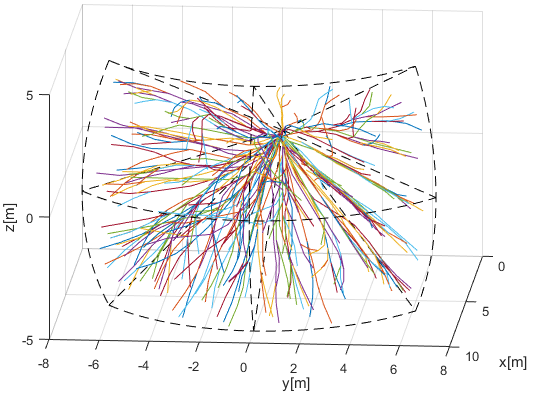
\includegraphics[width=0.7\linewidth]{\FIGDIR/RS004CombinedReachSetEstimationMethod} 
    \caption{\emph{Combined \emph{reach set} approximation}.}
    \label{fig:combinedReachSetApproximation}
\end{figure}


\paragraph{Pros and Cons:} It can bee seen from example (fig. \ref{fig:combinedReachSetApproximation}) that \emph{Combined Reach Set Approximation} (alg. \ref{alg:ReachSetMerge}) contains both types of maneuvers. \emph{Cheaper Smooth} for navigation and \emph{More Expensive Chaotic} for \emph{Emergency Avoidance}. The upper limit of trajectories is given as follow:

\begin{multline}
    countTrajectories(ReachSet) \le countTrajectories(Chaotic) \\+ countTrajectories(Harmonic)
\end{multline}

\noindent The \emph{upper limit of nodes} is given as follow:

\begin{equation}
    countNodes(ReachSet) \le countNodes(Chaotic)+ countNodes(Harmonic)
\end{equation}

\noindent \emph{Harmonic Reach Set} is ideal for \emph{Non-controlled Airspace} missions, because it contains \emph{Automatic Mode Switch} between \emph{Navigation} and \emph{Emergency Avoidance}.


\subsection{(R) ACAS-X like Reach set}\label{s:acasReachSet}
\paragraph{Motivation:} The implementation of \emph{ACAS-Xu} behavior in DAA system will  be mandatory for \emph{National Airspace System Integration} in United spaces \cite{shively2018uas}. 

Implementation of ACAS-Xu like behaviour increase usability of approach, if it can be achieved without major concept changes.


\paragraph{Background:} The \emph{ACAS-Xu} system on operational level has been described in \cite{marston2015acas}. The \emph{Policy for Collision Avoidance} proposal has been given in \cite{julian2016policy}.

Some behavioural patterns can be encoded into  \emph{Reach Set}. ACAS-Xu navigation part is basically \emph{Look-up table of Maneuvers for Allowed Separations}.
 
The \emph{Evasive Maneuver} selection process in ACAS-Xu is similar to our approach: \emph{Select most energy efficient maneuver in compliance with space-time constraints}. ACAS-Xu intruder model is similar to our \emph{Body Volume Intersection Model} (sec. \ref{s:bodyvolumeIntersection}). The \emph{ACAS-Xu} defines following base separations:

\begin{enumerate}
    \item \emph{Horizontal} - movements on \emph{Horizontal Plane} in \emph{Global Coordinate System}.
    
    \item \emph{Vertical} - movements on \emph{Vertical Plane} in \emph{Global Coordinate System}.
    
\end{enumerate}

\noindent There are allowed custom separations which can be used, for further experimentation: 
\begin{enumerate}
    \item \emph{Slash} - movement on $+45^{\circ}$ \emph{Tilted Plane to Horizontal Plane} in \emph{Global Coordinate System}.
    
    \item \emph{Backslash} - movement on $-45^{\circ}$ \emph{Tilted Plane to Horizontal Plane} in \emph{Global Coordinate System}.
    
\end{enumerate}

\noindent For given \emph{Movement Automaton} implementation (sec. \ref{s:modelMAImplementation}) the separations are given as follow:

\begin{equation}\label{eq:implementedseparations}
    \begin{aligned}
        Horizontal & = \{Straight, Left, Right \}\\
        Vertical & = \{Straight, Up, Down\}\\
        Slash & = \{Straight, UpLeft, DownRight\}\\
        Backslash & = \{Straight, UpRight, DownLeft\}\\
    \end{aligned}
\end{equation}

\noindent For each $Node(\dots,buffer)$ and each \emph{separation} there is a evaluation function $isSeparation$ which decides, if \emph{Trajectory} defined by node buffer is made up only from \emph{Separation} movements.  The function $isSeparation(\dots)$ is defined like:

\begin{equation}\label{eq:isSeparationPredicate}
    isSeparation(buffer,separation) =
    \begin{cases}
        \begin{aligned}
            \forall & movement \in buffer,\\ & movement \in separation
        \end{aligned}&: true\\
        otherwise &: false
    \end{cases}
\end{equation}

Following \emph{Separation Modes} can be defined with given \emph{separations}:

\begin{enumerate}
    \item \emph{Horizontal} (ACAS-X defined mode) containing \emph{horizontal} separation. 
    
    \item \emph{Vertical} (ACAS-X defined mode) containing \emph{vertical} separation.
    
    \item \emph{Horizontal-Vertical} (ACAS-X defined mode) containing \emph{horizontal, vertical} separations.
    
    \item \emph{Full} (custom defined mode) containing all \emph{Separation Modes}.
    
\end{enumerate}

\begin{note}
    Every separation modes generates 2D trajectories set on \emph{Respective plane}. There is no need for \emph{Tuning parameters} for further \emph{Expansion Constraint}.    
\end{note}

\paragraph{Expansion Constraint Function Implementation} (alg. \ref{alg:ExpansionConstraintFunctionForACASLikeReachSet}) is based on simple principle:
\emph{Select only candidate Nodes which Trajectories have at least one desired Separation Mode}.

\paragraph{Step: Initialization} sets candidate \emph{Nodes} as empty set,  leftover \emph{Nodes} as empty set, and, select all nodes form \emph{stack} which represents \emph{Finishing Trajectories} in working $cell_{i,j,k}$,

\paragraph{Step: Candidate Selection Process} is evaluated for each \emph{test Node} from \emph{passing Node Set}. 

For each \emph{applicable separation}, given as input parameter \emph{separations}, The test function \emph{isSeparation} (eq. \ref{eq:isSeparationPredicate}) is applied:
\begin{enumerate}
    \item If \emph{test Node} trajectory belongs to at least one allowed separation it is added to candidates set.
    \item Else is added to \emph{Leftovers}.
\end{enumerate}

\begin{note}
    \emph{Separation sets} (eq. \ref{eq:implementedseparations}) are not \emph{exclusive sets} in \emph{Movement Automaton} domain. One \emph{Trajectory} contained by Node can belong to multiple \emph{Separations}.    
\end{note}

\begin{algorithm}[H]
\SetKwInOut{Input}{Input}\SetKwInOut{Output}{Output}\SetKwInOut{TuningParameters}{Tuning Parameters}
    \Input{Node[] stack, Cell cell$_{i,j,k}$, Separation[] separations}
    \TuningParameters{$None:\varnothing$}
    \Output{Node[] candidates, Node[] leftovers}
    
    \BlankLine
    \# Initialize structures\;
    Node[] candidates = [], Node[] leftovers=[]\;
    Node[] passing = cell$_{i,j,k}$.getFinishingTrajectories(stack)\;
    
    \BlankLine
    \# Select nodes containing trajectories with usable separations\;
    \For{Node test $\in$ passing}{
        \For{separation $\in$ separations}{
            \BlankLine
            \# Get separations for Node\;
            Separations[] nodeSeparations = test.getSeparations()\;
            \BlankLine
            \# If trajectory given by buffer is on Separation plane\;
            \If{isIn(isSeparation(test.buffer,separation)(\ref{eq:isSeparationPredicate})}{
                candidates.append(test)\;
            }
        }
        \BlankLine
        \# If there was no applicable separation, throw Node away\;
        \If{test $\not\in$ candidates}{
            leftovers.append(test)\;
        }
    }
    \BlankLine
    \# Return results\;
    \Return{[candidates,leftovers]}
    
    \caption{Expansion Constraint function for \emph{ACAS-like Reach Set Approximation}}
    \label{alg:ExpansionConstraintFunctionForACASLikeReachSet}    
\end{algorithm}

\paragraph{Example:} for \emph{Avoidance Grid} with \emph{Distance 10 m}, \emph{Layer count 10}, \emph{Horizontal range $[-45^\circ,+45^\circ]$}, \emph{Horizontal Cell Count 7}, \emph{Vertical range $[-30^\circ,+30^\circ]$}, and \emph{Vertical Cell Count 5}. Is given in (fig. \ref{fig:acasLikeReachSetVariousSeparationMode}). The UAS is at \emph{Back-side} of \emph{Figure} (initial state is at all \emph{Trajectory Origins}). The \emph{black dashed line} marks \emph{Avoidance Grid} space boundary. Each trajectory has its own color and ends at \emph{Front-side} of \emph{Avoidance Grid Boundary}.

\emph{Full} separation mode given in (fig. \ref{fig:acasLikeReachSetFull}). \emph{Horizontal-Vertical} separation mode, used in original \emph{ACAS-Xu} testing \cite{marston2015acas}, given in (fig. \ref{fig:acasLikeReachSetHorizontalVertical}). \emph{Horizontal} separation mode given in (fig. \ref{fig:acasLikeReachSetHorizontalOnly}) is usually used by planes. \emph{Vertical} separation mode given in (fig. \ref{fig:acasLikeReachSetVerticalOnly}) is usually used by copters.

\begin{figure}[H]
	\centering
    \begin{subfigure}{0.48\textwidth}
        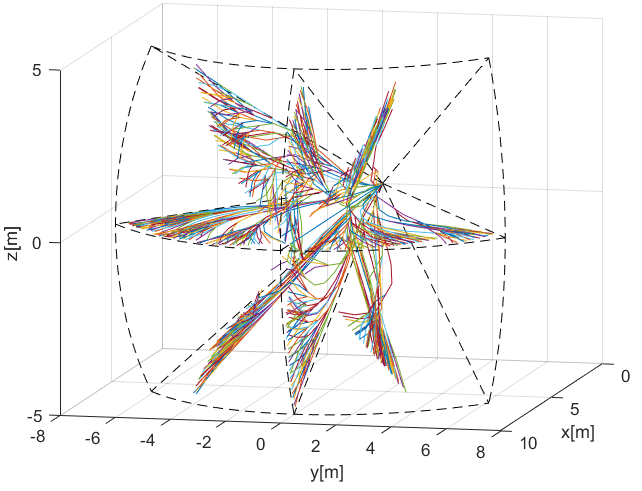
\includegraphics[width=0.9\linewidth]{\FIGDIR/RS005ACASLikeReachSetEstimationMethodFull}
        \caption{Full.}
        \label{fig:acasLikeReachSetFull}
    \end{subfigure}
    \begin{subfigure}{0.48\textwidth}
        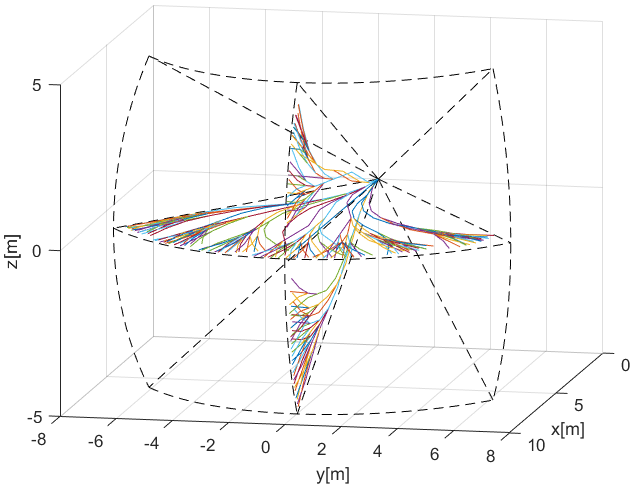
\includegraphics[width=0.9\linewidth]{\FIGDIR/RS006ACASLikeReachSetEstimationMethodHorizontalVertical} 
        \caption{Horizontal-Vertical.}
        \label{fig:acasLikeReachSetHorizontalVertical}
    \end{subfigure}
    \\
    \begin{subfigure}{0.48\textwidth}
        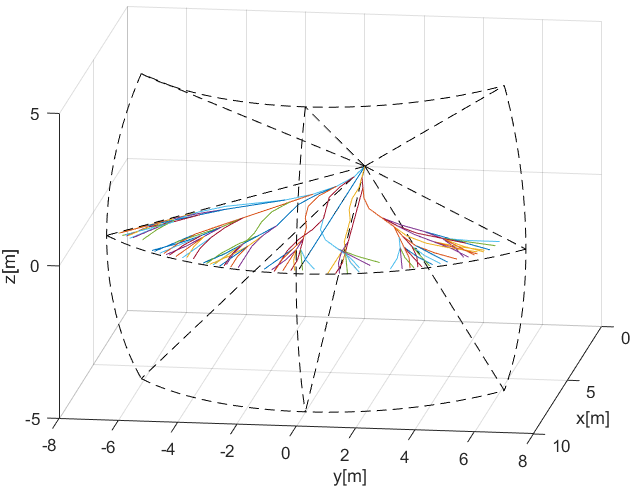
\includegraphics[width=0.9\linewidth]{\FIGDIR/RS008ACASLikeReachSetEstimationMethodHorizontal} 
        \caption{Horizontal.}
        \label{fig:acasLikeReachSetHorizontalOnly}
    \end{subfigure}
    \begin{subfigure}{0.48\textwidth}
        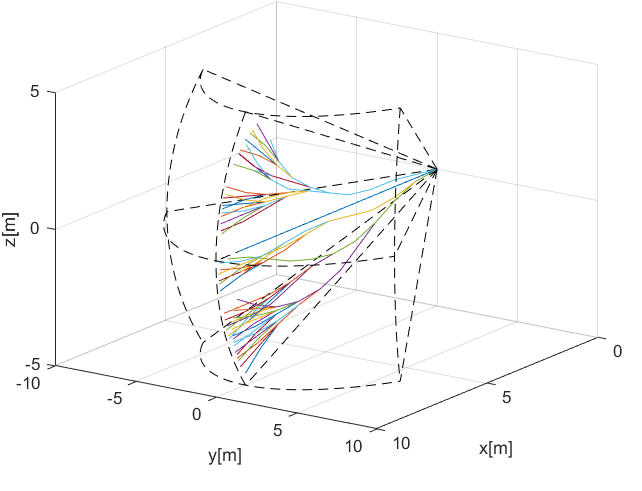
\includegraphics[width=0.9\linewidth]{\FIGDIR/RS009CASLikeReachSetEstimationMethodVertical} 
        \caption{Vertical.}
        \label{fig:acasLikeReachSetVerticalOnly}
    \end{subfigure}
    \caption{ACAS-X imitation \emph{reach set} approximation for various \emph{separation modes}. }
    \label{fig:acasLikeReachSetVariousSeparationMode}
\end{figure}

\paragraph{Pros and Cons:} It can be seen from examples (fig. \ref{fig:acasLikeReachSetVariousSeparationMode}) that \emph{ACAS-like Reach Set Approximation Method} (alg. \ref{alg:ExpansionConstraintFunctionForACASLikeReachSet}) generates full reach set for 2D plane located in 3D space. 

The \emph{Reach Set} contains trajectories with \emph{high coverage ratio} and \emph{high smoothness rating} for selected 2D separation plane. Overall performance compared to full 3D reach sets (sec. \ref{s:chaoticReachSet}, \ref{s:harmonicReachSet} \ref{s:combinedReachSet}) is poor. 

The \emph{node} and \emph{trajectory} count boundary was not implemented. It is common knowledge that \emph{2D} avoidance sets does not require scaling \cite{marston2015acas}. Otherwise trajectory footprint mechanism like in \emph{Harmonic Reach Set Approximation} (alg. \ref{alg:ExpansionConstraintFunctionForHarmonicReachSet}) can be introduced.

This reach set implements \emph{Planar-Separation} as native feature, it can be used for both \emph{navigation} and \emph{avoidance} tasks in \emph{Controlled Airspace}. For \emph{Non-controlled Airspace} there are far more superior \emph{Combined Reach Set} (sec. \ref{s:combinedReachSet}).

	
    %06-04 Static Obstacles and Constraints
    \cleardoublepage
\section{\secState{R}Static Obstacles and Constraints}\label{s:staticObstacles}
    
\paragraph{Introduction:} The \emph{static obstacles} were used in original concept \cite{gomola2017probabilistic}, the \emph{Avoidance Grid} and \emph{Movement Automaton} were repurposed to enable \emph{finite time deterministic} avoidance. An \emph{Constraint based path search} and \emph{obstacle modeling} is summarized in \cite{hentenryck2009constraint}.

This section is handling basic problems of \emph{static obstacle} detection and its focused on following real-world fixed position threats:
\begin{enumerate}
    \item \emph{Static Obstacles} - detected by LiDAR sensor or fused from \emph{Obstacle Map} information source.
    
    \item \emph{Geo-fencing Areas} - defined by offline/online information source as permanent flight restriction zones. There is usually no physical obstacle. The space is considered as \emph{hard/soft constraint}.
    
    \item \emph{Long-term bad weather Areas} - the \emph{weather} is changing often (hour period), there are \emph{weather events}  which lasts for \emph{hours} or \emph{days}.
\end{enumerate}


\paragraph{Changing Scanning Density of LiDAR:} A LiDAR sensor is scanning in conic section given by $distance Range$, $horizontal Range$, $vertical Range$, where distance range is in interval $[0,maxDistance]$, horizontal offset range is in $[-pi,pi]$, and vertical offset range is in $[\varphi_s, \varphi_e]$.  

Let say that $\text{d} horizontal^\circ, \text{d} vertical^\circ$ is unitary angle offset in which one LiDAR send and return is executed. That means the \emph{LiDAR} ray is sent every $\text{d} horizontal^\circ, \text{d} vertical^\circ$ offset movement. The \emph{LiDAR} ray density is decreasing with \emph{distance offset}. The same amount of \emph{LiDAR} rays passes trough $cell_{i,j,k}$ in Avoidance Grid.

The surface of area given by some distance d, and unitary offsets$\partial horizontal^\circ, \text{d} vertical^\circ$  is changing with $distance$. The minimal triggering area of object surface is not changing. This fact has an impact on count of the hits on object surface. 

The example is given in (fig. \ref{fig:P01CountOfLiDARHits}) where we have two identical objects (red circle) in distances 5 and 10 meters. The closer object consumes 5 LiDAR beam hits and the farther object consumes only 3 LiDAR beam hits. The probability of obstacle encounter is remaining the same for closer and farther object. The \emph{detected obstacle rate} assessment should return the same  detected obstacle collision rate for objects with same scanned surface (with different LiDAR ray hit count).

\begin{figure}[H]
    \centering
    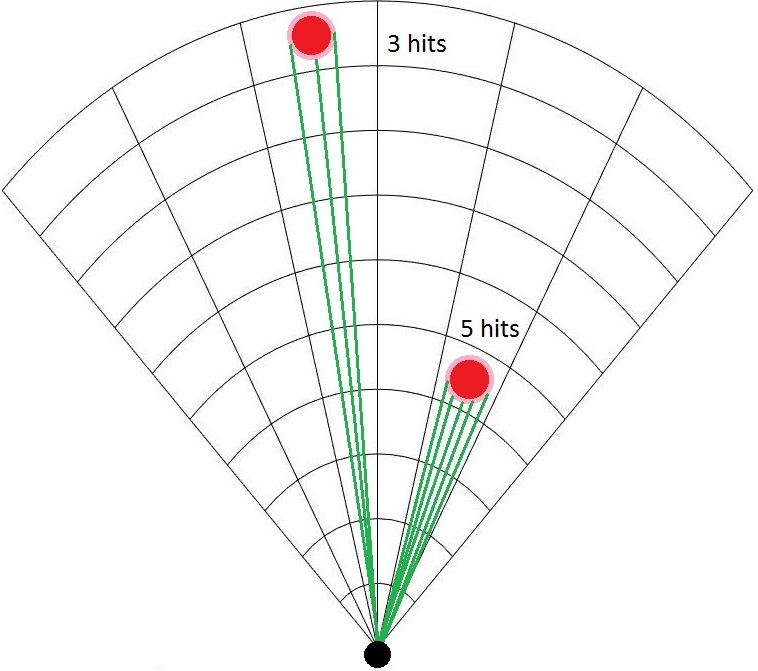
\includegraphics[width=0.7\textwidth]{\FIGDIR/TE051CountOfLiDARHits}
    \caption{Different count of LiDAR hits with different distance from UAS.}
    \label{fig:P01CountOfLiDARHits}
\end{figure}


\paragraph{Map and Detected Obstacles Fusion:} The concept of \emph{offline/online obstacle map} is mandatory in modern obstacle avoidance systems and increases the safety of navigation/avoidance path. The \emph{older} concept was considering only LiDAR reading or \emph{real-time sensor readings} in general \cite{gomola2017probabilistic}. 

\begin{figure}[htbp]
    \centering
    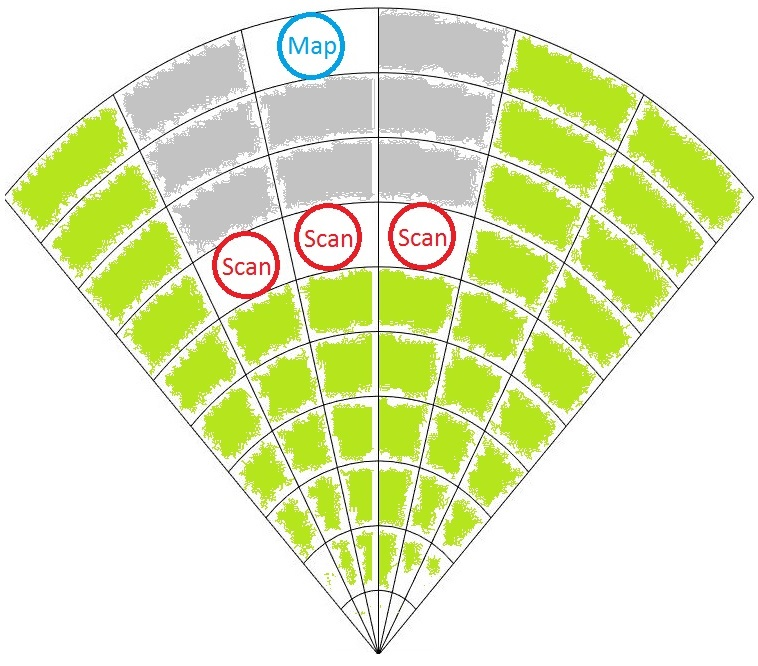
\includegraphics[width=0.7\textwidth]{\FIGDIR/TE053OvershadowedMapobstacle}
    \caption{Overshadowed map obstacle by detected obstacles.}
    \label{fig:P02OvershadowedMapobstacle}
\end{figure}

\newpage\noindent The fusion of real time sensor readings and obstacle map (prior knowledge) is required. Data fusion of these two sources is strongly depending on visibility property, because there are three basic scenarios:

\begin{enumerate}
    \item \emph{Dual detection} - the obstacle is marked on the map and detected by sensory system at some point of the time (older concept works).
    
    \item \emph{Hindered vision} - the detected obstacles are hindering vision to map obstacle therefore map obstacle uncertainty arises (older concept fails). 
    
    \item \emph{False-positive map} - map obstacle occupied space is visible by sensory system, but negative detection is returned. Therefore the map is giving \emph{false-positive} information.
\end{enumerate}

\noindent The second case is given in fig. \ref{fig:P02OvershadowedMapobstacle}, where map obstacle (blue circle) is overshadowed by three scanned obstacles (red circle). The visible space is denoted by green fill, the invisible space is denoted by gray fill. 
    	\subsection{(R) Detected obstacles}\label{s:detectedObstacles}
\paragraph{Idea:} The \emph{visibility} inside avoidance grid and \emph{obstacle} probability are interconnected for most ranging sensors (ex. LiDAR). The goal of this section is to introduce \emph{visibility hindrance} concept which includes space uncertainty assessment and detected obstacle  processing.

\paragraph{Detected Obstacle Rating:} The \emph{detected obstacle rating} defines UAS chances to encounter detected obstacle in avoidance grid $cell_{i,j,k}$. Final \emph{detected obstacle rating} is merged information (eq. \ref{eq:detectedObstacleRatingForCell}). The \emph{sensor field} can contain \emph{multiple} \emph{static obstacle sensors}.

\paragraph{Detected Obstacle Rate for LiDAR:},Lets have only one sensor set as homogeneous two axis rotary LiDAR. For one $cell_{i,j,k}$ there exists set of passing LiDAR beams:

\begin{equation}\label{eq:lidarRaysTroughCell}
    lidar Rays(cell_{i,j,k})=
    \left\{
        \begin{aligned}
        \left[
            \begin{gathered}
                horizontal^\circ\in horizontal Offsets,\\
                vertical^\circ\in vertical Offsets
            \end{gathered}
        \right]\in\R^2:&\\
        horizontal^\circ\in cell_{i,j,k}.horizontal &Range,\\
        vertical^\circ\in cell_{i,j,k}.vertical &Range\\
        \end{aligned}
    \right\}
\end{equation}

\noindent The horizontal and vertical offset of LiDAR ray is homogeneous. Meaning the horizontal/vertical distances between each two neighbouring LiDAR beams are equal.

The set $lidar Rays(cell_{i,j,k}))$ (eq. \ref{eq:lidarRaysTroughCell}) is finite countable and nonempty for any $c_{i,j,k}$, otherwise it will contradict   the definition of avoidance grid (def. \ref{def:AvoidanceGrid}).

The hit function $lidarScan()$ returns a distance of single beam return for beam with dislocation $[horizontal^\circ,$ $vertical^\circ]$ $\in$ $lidar Rays(cell_{i,j,k})$ angle offsets. The set of LiDAR hits (eq. \ref{eq:lidarHitFunction}) in cell $cell_{i,j,k}$ is defined like follow:

\begin{equation}\label{eq:lidarHitFunction}
    lidar Hits(cell_{i,j,k})=\left\{
        \begin{aligned}
        \left[
            \begin{gathered}
                distance=lidar Scan(),\\
                horizontal^\circ\in horizontal Offsets,\\
                vertical^\circ\in vertical Offsets
            \end{gathered}
        \right]\in\R^2:&\\
        distance \in cell_{i,j,k}.distance &Range,\\
        horizontal^\circ\in cell_{i,j,k}.horizontal &Range,\\
        vertical^\circ\in cell_{i,j,k}.vertical &Range\\
        \end{aligned}
    \right\}
\end{equation}

\noindent The \emph{naive} obstacle rate in case of LiDAR sensor defined as ratio between landed hits and possible hits:

\begin{equation}\label{eq:naiveObstacleRate}
    obstacle^{LiDAR}_{cell_{i,j,k}}=\frac{lidar Hits(cell_{i,j,k})}{lidar Rays(cell_{i,j,k})}
\end{equation}

\begin{note}
    The \emph{naive obstacle rate} (eq. \ref{eq:naiveObstacleRate}) ignores that \emph{LiDAR rays} are getting more far apart from each other. The \emph{cell surface} is increasing with cell distance from \emph{UAS}.
\end{note}

\noindent The hindrance (eq. \ref{eq:probabilityOfVisibilityHindrance}) rate is naturally defined as supplement to naive obstacle rate. This definition is sufficient, because its reflecting the \emph{remaining sensing capability} of  LiDAR.

\begin{equation}\label{eq:probabilityOfVisibilityHindrance}
    hindrance^{LiDAR}_{cell_{i,j,k}}=1-\frac{lidar Hits(cell_{i,j,k})}{lidar Rays(cell_{i,j,k})}
\end{equation}

\paragraph{Cell Density Function:}  Let`s start with differential form of cell surface (eq. \ref{eq:finalCellSquare}). The target object have several hits in \emph{Avoidance Grid}. Target $cell_{i,j,k}$ has following properties which are used in surface calculation:
\begin{enumerate}
    \item \textit{Horizontal span} - defines range of horizontal scanner partition.
    \item \textit{Vertical span} - defines range of vertical scanner partition.
\end{enumerate}

\noindent By rewriting (eq. \ref{eq:finalCellSquare}) and using horizontal range parameter and inverted vertical range parameter following surface integral is obtained (eq. \ref{eq:cellSurfaceIntengralDelta}).

\begin{multline}\label{eq:cellSurfaceIntengralDelta}
    Area(cell_{i,j,k}) =\\ \int_{horizontal_{start}^\circ}^{horizontal_{end}^\circ}\int_{vertical_{end}^\circ}^{vertical_{start}^\circ} radius^2 \cos(vertical^\circ) \quad \text{d} vertical^
    \circ\text{d} horizontal^\circ
\end{multline}

\begin{note}
    The \emph{radius} parameter is \emph{average} distance of hits landed in $cell_{i,j,k}$. This helps to reflect real \emph{scanned surface}.
\end{note}

Numerically stable integration exist for boundaries $horizontal^\circ \ in [-\pi,\pi]$, $vertical^\circ \in [-\frac{\pi}{2},\frac{\pi}{2}]$ given as follow:

\begin{multline}\label{eq:intersectionSurfaceForCell}
    Area(radius,horizontal Range, vertical_{start}^\circ, vertical_{end}^\circ) =\dots\\ 
    =\left\{
    \begin{aligned}
        vertical&_{start}^\circ <0, vertical_{end}^\circ \le 0 :\\ 
            &radius^2(\sin |vertical_{start}^\circ| - \sin|vertical_{end}^\circ|)\times horizontal Range)\\
         vertical&_{start}^\circ <0, vertical_{end}^\circ > 0   :\\
            & r^2(\sin |vertical_{start}^\circ| + \sin|vertical_{end}^\circ|)\times horizontal Range)\\
         vertical&_{start}^\circ \ge 0 vertical_{end}^\circ < 0 :\\
            & r^2(\sin vertical_{end}^\circ- \sin vertical_{start}^\circ)\times horizontal Range)
    \end{aligned}
    \right.
\end{multline}

\noindent An intersection surface for cell is defined in (eq. \ref{eq:intersectionSurfaceForCell}). Area covered by LiDAR hits (eq. \ref{eq:lidarHitArea}) is defined as LiDAR hit rate (hits to passing rays ratio) multiplied by \emph{Average} cell intersection surface (eq. \ref{eq:intersectionSurfaceForCell}).

\begin{equation}\label{eq:lidarHitArea}
    lidar Hit Area(cell_{i,j,k}) = \frac{lidar Hits(cell_{i,j,k})}{lidar Rays(cell_{i,j,k})} \times Area\left(\begin{gathered}radius,horizontal Range,\\ vertical_{start}^\circ, vertical_{end}^\circ\end{gathered}\right)
\end{equation}

\noindent There is user defined parameter for \emph{LiDAR treshold area}, which represents minimal considerable surface area for obstacle to be threat. The \emph{detected obstacle rate} considering surface is defined in (eq. \ref{eq:lidarHitFormula}) and it removes bias of naive approach (eq.\ref{eq:naiveObstacleRate}).

\begin{equation}\label{eq:lidarHitFormula}
    obstacle(LiDAR,cell_{i,j,k})=\min\left\{\frac{lidar Hit Area(cell_{i,j,k})}{UAS.lidar Threshold Area},1\right\}
\end{equation}



\paragraph{Visibility Rate for  LiDAR:} For each $cell_{i,j,k}$ and each sensor in sensor field there exist hindrance rate, which defines how much vision is clouded in single cell. Example of hindrance calculation for LiDAR has been given by (eq. \ref{eq:probabilityOfVisibilityHindrance}). Let us consider cell row $cell Row (j_{fix},$ $k_{fix})$ with fixed horizontal index $j_fix$ and vertical index $k_{fix}$ is given as series of cells (eq. \ref{eq:cellrowDefinition}).

\begin{equation}\label{eq:cellrowDefinition}
    cellRow(j_{fix},k_{fix})= \left\{cell_{i,j,k}\in Avoidance Grid :\begin{aligned}&i\in\{1,..,layersCount\},\\&j=j_{fix}, k=k_{fix}\end{aligned}\right\}
\end{equation}

For each $cell_{i,j,k}$ there exists a function which calculates final visibility hindrance rate. Then for ordered cell row:
\begin{equation*}
    cell Row(j_{fix},k_{fix}) = \{cell_{1,j_{fix},k_{fix}},  cell_{2,j_{fix},k_{fix}}, \dots, cell_{layers Count,j_{fix},k_{fix}}\}    
\end{equation*}
and for one selected $cell_{i,j,k}$ the visibility rate is naturally defined as a supplement to hindrance from previous cells. The visibility is defined in (eq. \ref{eq:FinalVisibilityProbability}).

\begin{multline}\label{eq:FinalVisibilityProbability}
    visibility(cell_{i_c,j_c,k_c})=\dots\\ \dots =1 - \sum_{index\in\N^+}^{index < i_c} hindrance(cell_{a,j_c,k_c}: cell_{a,j_c,k_c}\in cell Row(j_{c},k_{c})
\end{multline}

\paragraph{Example:} Let be $cell_{4,j_{fix},k_{fix}}$ is selected for visibility rate assessment, then $cell_{1,j_{fix},k_{fix}}$, $cell_{2,j_{fix},k_{fix}}$, and $cell_{3,j_{fix},k_{fix}}$, are used as a base of cumulative hindrance rate.

\noindent \emph{The cumulative hindrance rate} for any $cell Row(j_{fix},k_{fix})$ is bounded:

\begin{equation}
    0 \le \sum_{cell\in cell Row(j_{fix},k_{fix})} visibility(cell) \le 1
\end{equation}

\begin{note}
    A \emph{cumulative hindrance rate} does not always reach 1 in case of LiDAR sensor, because some rays may pass or hit after leaving \emph{avoidance grid} range.
\end{note}


\begin{figure}[H]
    \centering
    \begin{subfigure}{0.32\textwidth}
        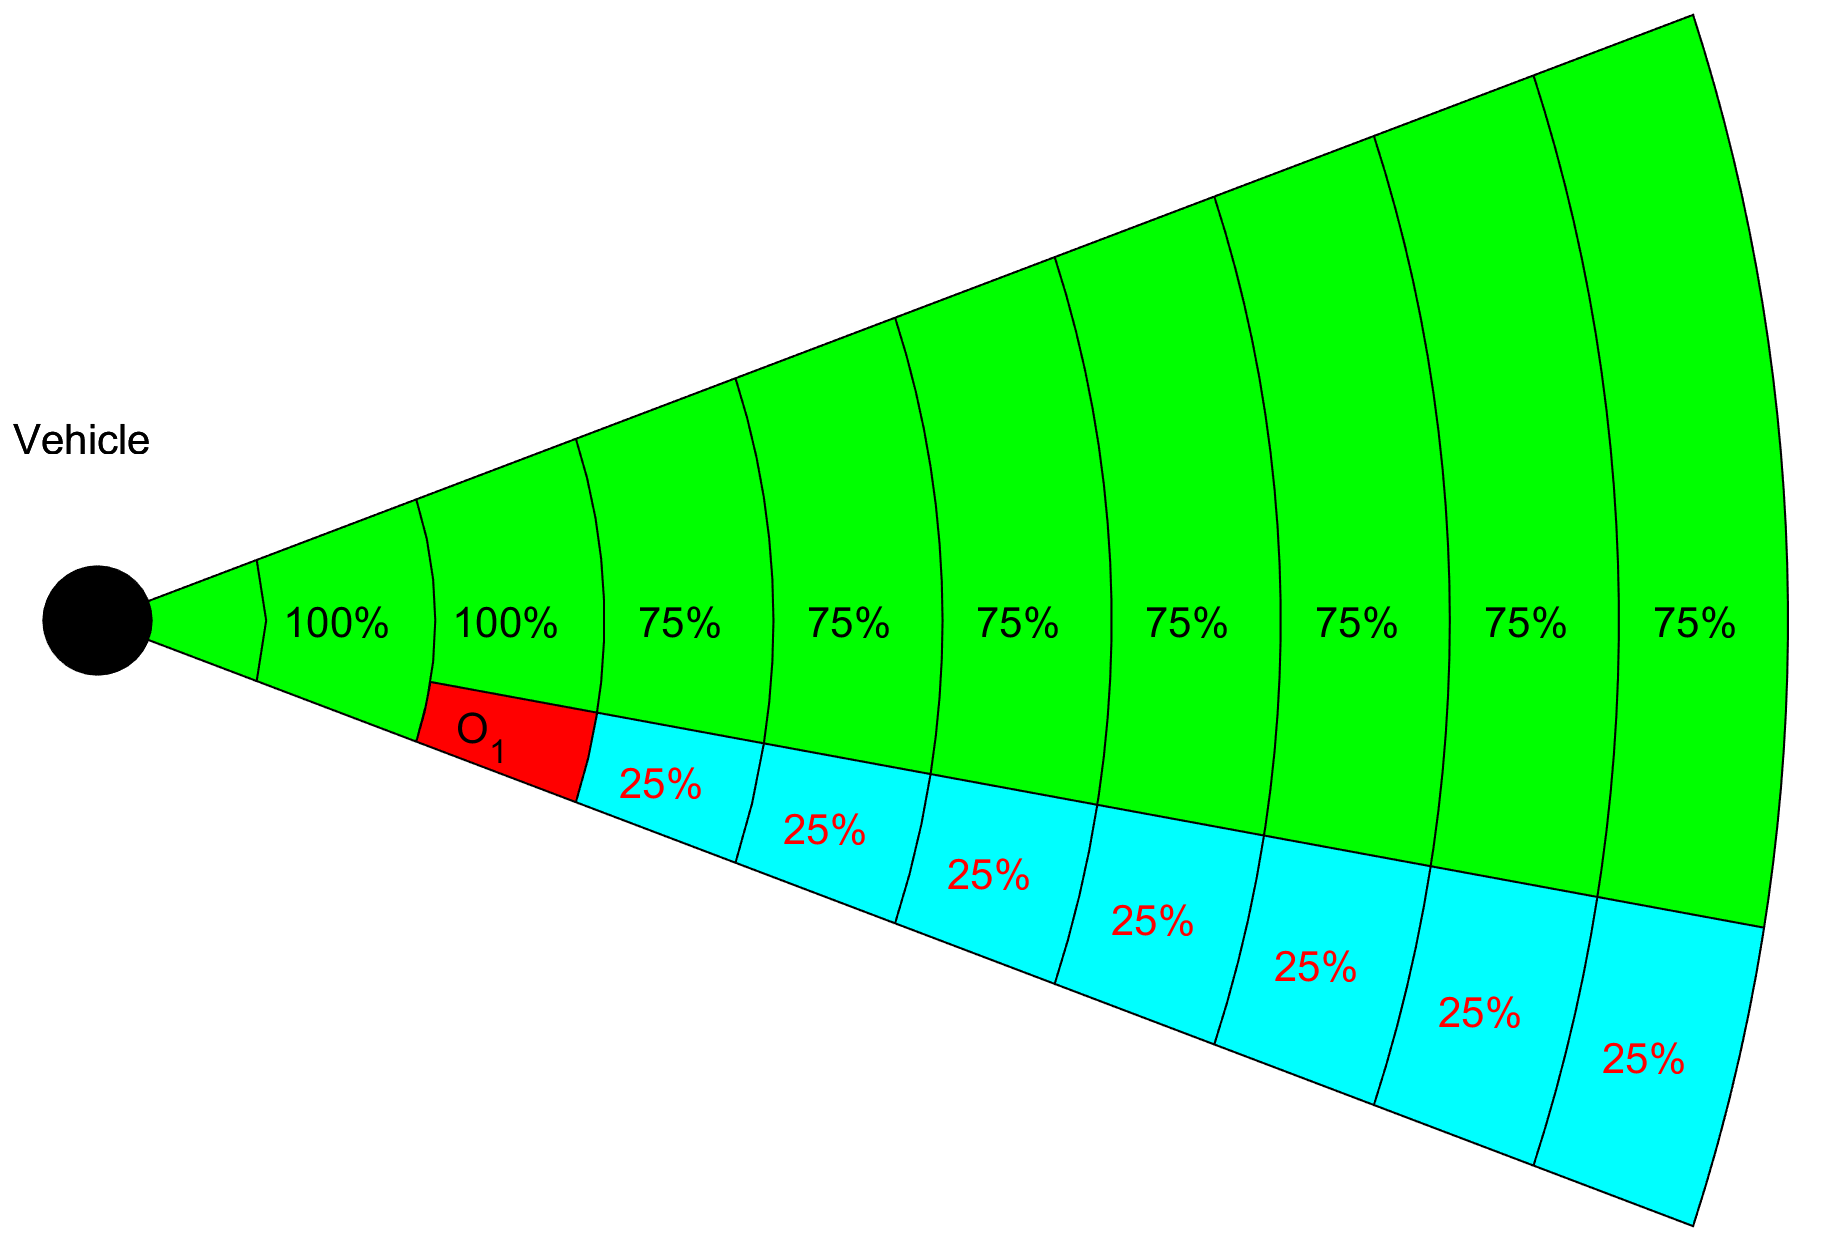
\includegraphics[width=0.9\linewidth]{\FIGDIR/TE006VisibilityFirstObstacle} 
        \caption{1\textsuperscript{st} hindrance.}
        \label{fig:fistObstacleHindrance}
    \end{subfigure}
    \begin{subfigure}{0.32\textwidth}
        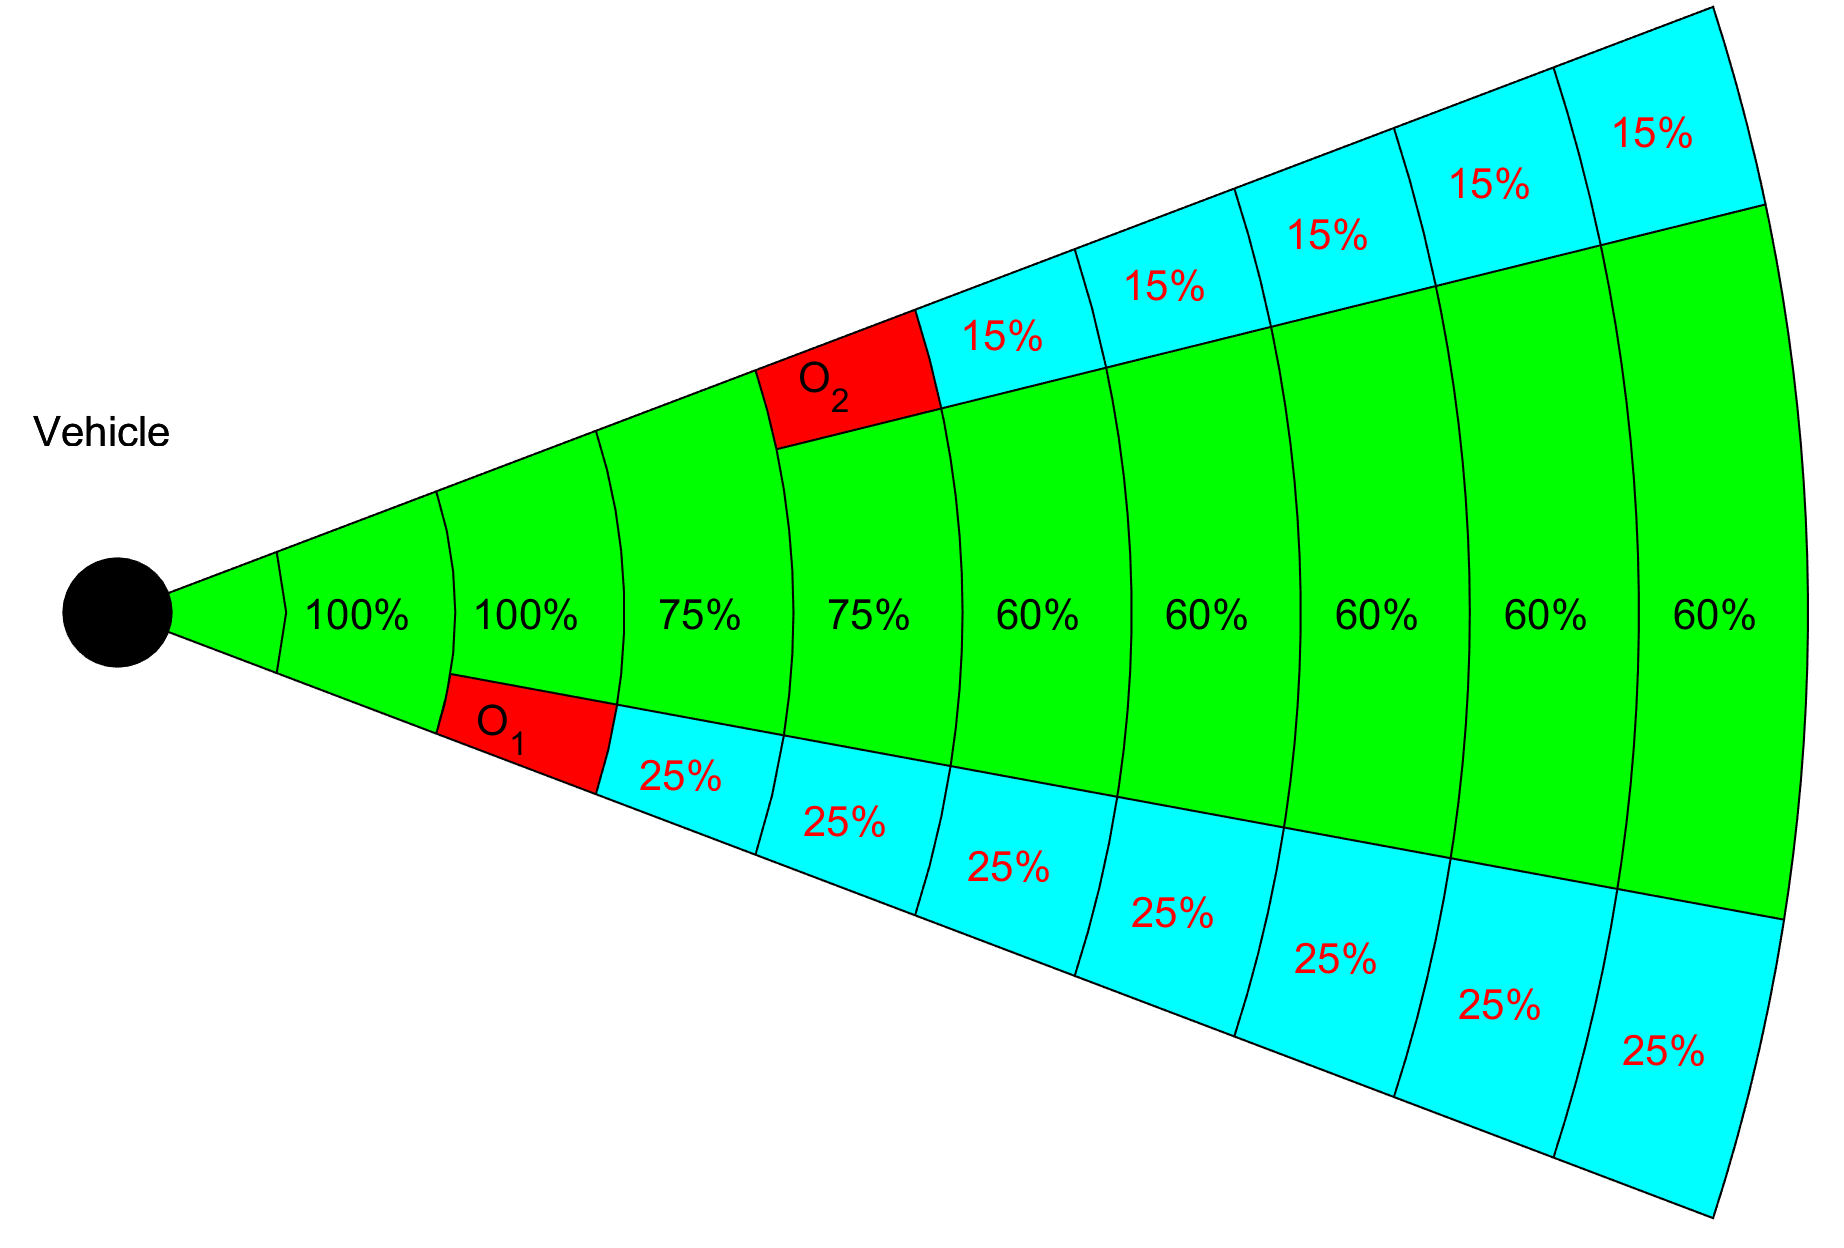
\includegraphics[width=0.9\linewidth]{\FIGDIR/TE007VisibilitySecondObstacle} 
        \caption{2\textsuperscript{nd} hindrance.}
        \label{fig:secondObstacleHindrance}
    \end{subfigure}
    \begin{subfigure}{0.32\textwidth}
        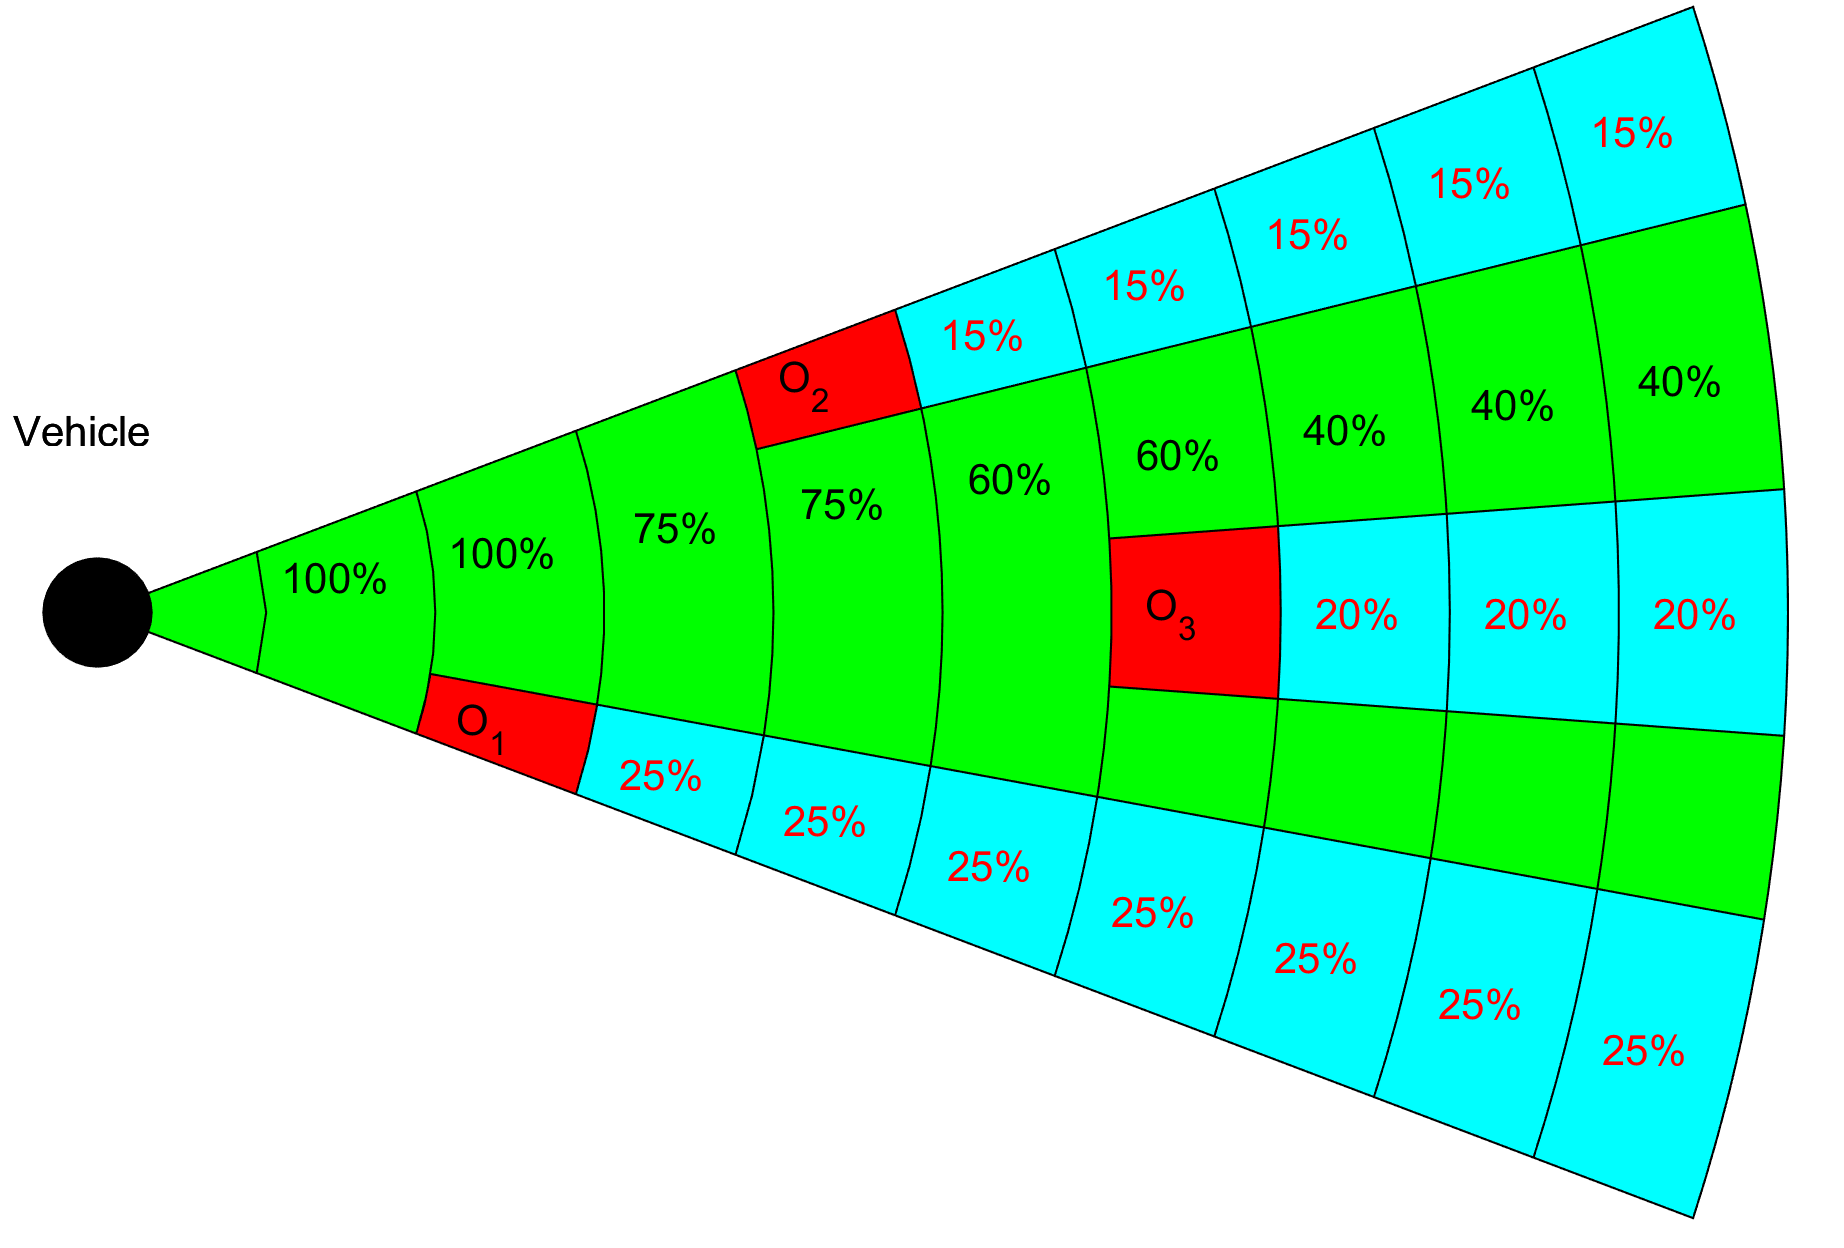
\includegraphics[width=0.9\linewidth]{\FIGDIR/TE008VisibilityThirdObstacle} 
        \caption{3\textsuperscript{rd} hindrance.}
        \label{fig:thirdObstacleHindrance}
    \end{subfigure}
    \caption{Obstacle hindrance impact on visibility in \emph{Avoidance Grid Slice}.}
    \label{fig:hindranceImpactOnVisibility}
\end{figure}

For one cell row $cell Row(j_{fix},k_{fix})$, where count of layers is equal to 10, and layers have equal spacing. There is LiDAR sensor

During consequent LiDAR scans $s(t_0)$, $s(t_1)$, $s(t_2)$, and $s(t_3)$ the obstacle sets $\mathscr{O}_1(t_1)=\{o_1\}$, $\mathscr{O}_2(t_2)=\{o_1,o_2\}$, and $\mathscr{O}_3(t_3)=\{o_1,o_2,o_3\}$ are discovered. Assigned hindrance rates are like follow:

\begin{enumerate}
    \item\emph{Time $t_0$} - there is no obstacle nor hindrance, all cells are fully visible.

    \item\emph{Time $t_1$} (fig. \ref{fig:fistObstacleHindrance}) - $\mathscr{O}_1(t_1)=\{o_1\}$ was detected, the hindrance rate  for $cell_{3,j_{fix},k_{fix}})$ is equal to $0.25$. The visibility rate in cells $cells_{4-10,j_{fix},k_{fix}}$ is $0.75$. 
    
    \item\emph{Time $t_2$} (fig. \ref{fig:secondObstacleHindrance}) - $\mathscr{O}_2(t_2)=\{o_1,o_2\}$ was detected, the additional hindrance rate for $cell_{5,j_{fix},k_{fix}}$ is $0.15$. The visibility rate in  $cells_{6-10,j_{fix},k_{fix}}$ is lowered by additional $0.15$ and its set to $0.60$ now.
    
    \item\emph{Time $t_3$} (fig. \ref{fig:thirdObstacleHindrance}) - $\mathscr{O}_3(t_3)=\{o_1,o_2,o_3\}$  was detected the additional hindrance rate for  $cell_{7,j_{fix},k_{fix}}$ is $0.20$. The visibility rate in $cells_{8-10,j_{fix},k_{fix}}$ is lowered by additional $0.20$ and its set to $0.40$  now.
\end{enumerate}
		%\subsection{\secState{R}Map Obstacles}\label{s:mapObstacles}
\paragraph{Map Obstacles:} Use \emph{stored LiDAR readings} from previous mission to build an compact obstacle map \cite{cernamaria2018}. Then use \emph{this map} as a additional information source.

\begin{figure}[H]
    \begin{subfigure}{0.32\textwidth}
        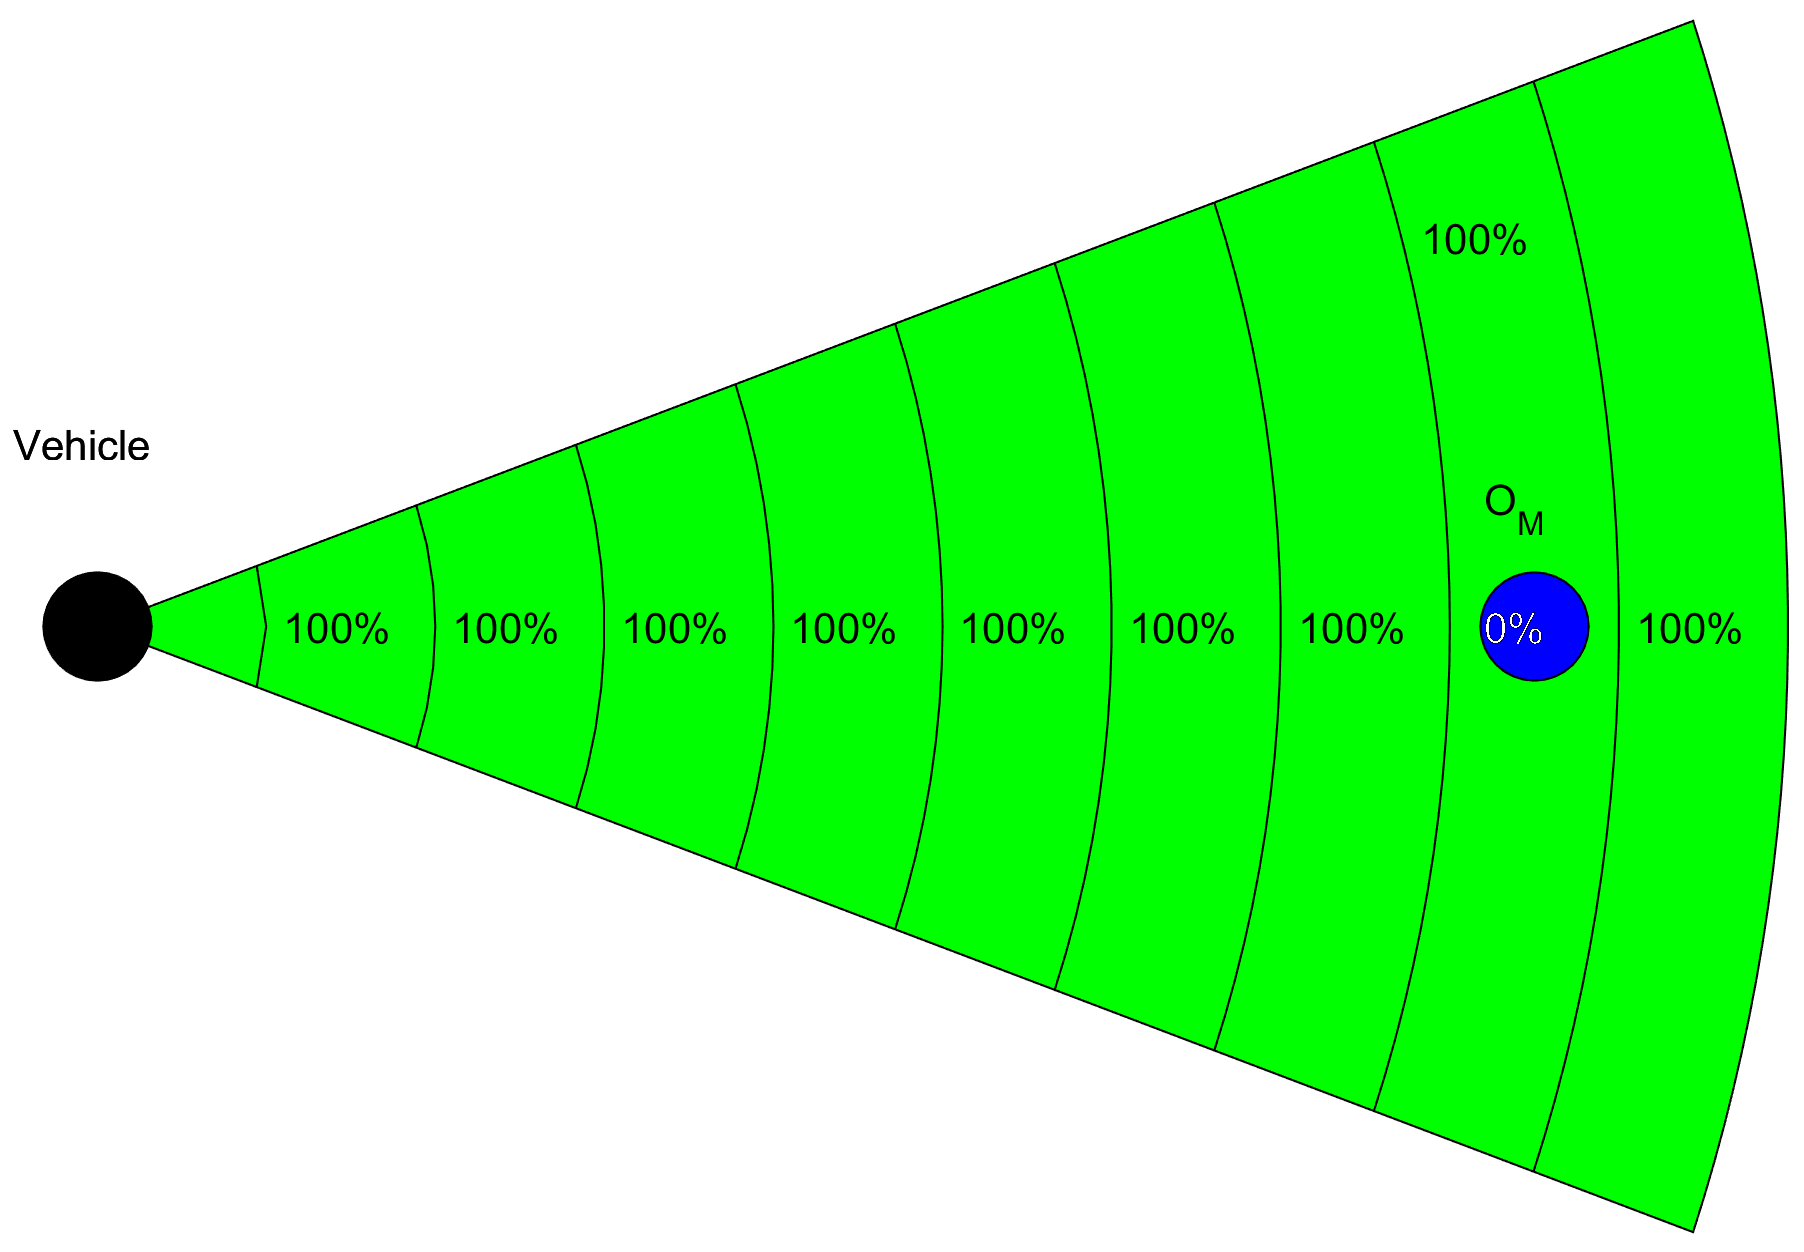
\includegraphics[width=0.9\linewidth]{\FIGDIR/TE009MapObstacleUndetected} 
        \caption{Undetected.}
        \label{fig:undetectedMapObstalce}
    \end{subfigure}
    \begin{subfigure}{0.32\textwidth}
        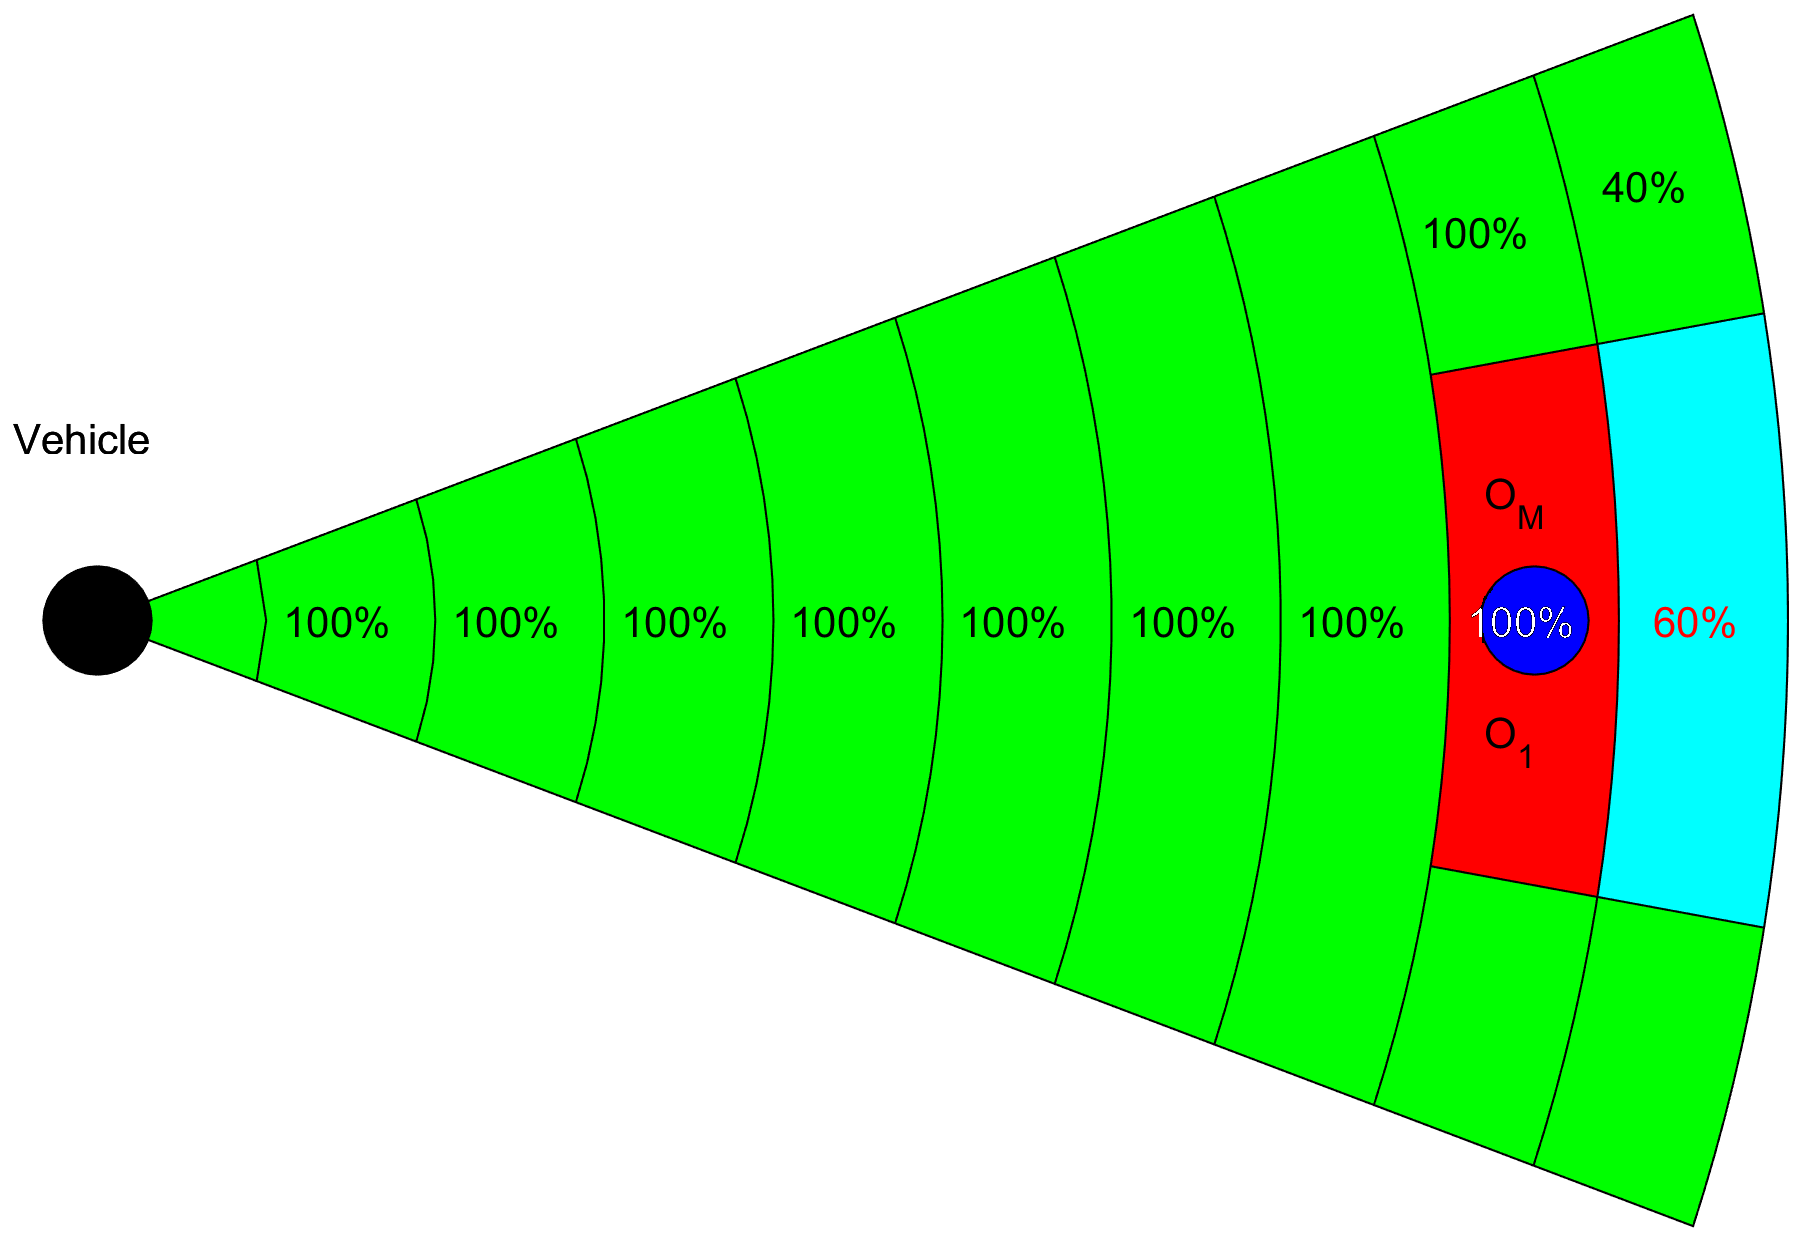
\includegraphics[width=0.9\linewidth]{\FIGDIR/TE010MapObstacleDetected} 
        \caption{Detected.}
        \label{fig:detectedMapObstacle}
    \end{subfigure}
    \begin{subfigure}{0.32\textwidth}
        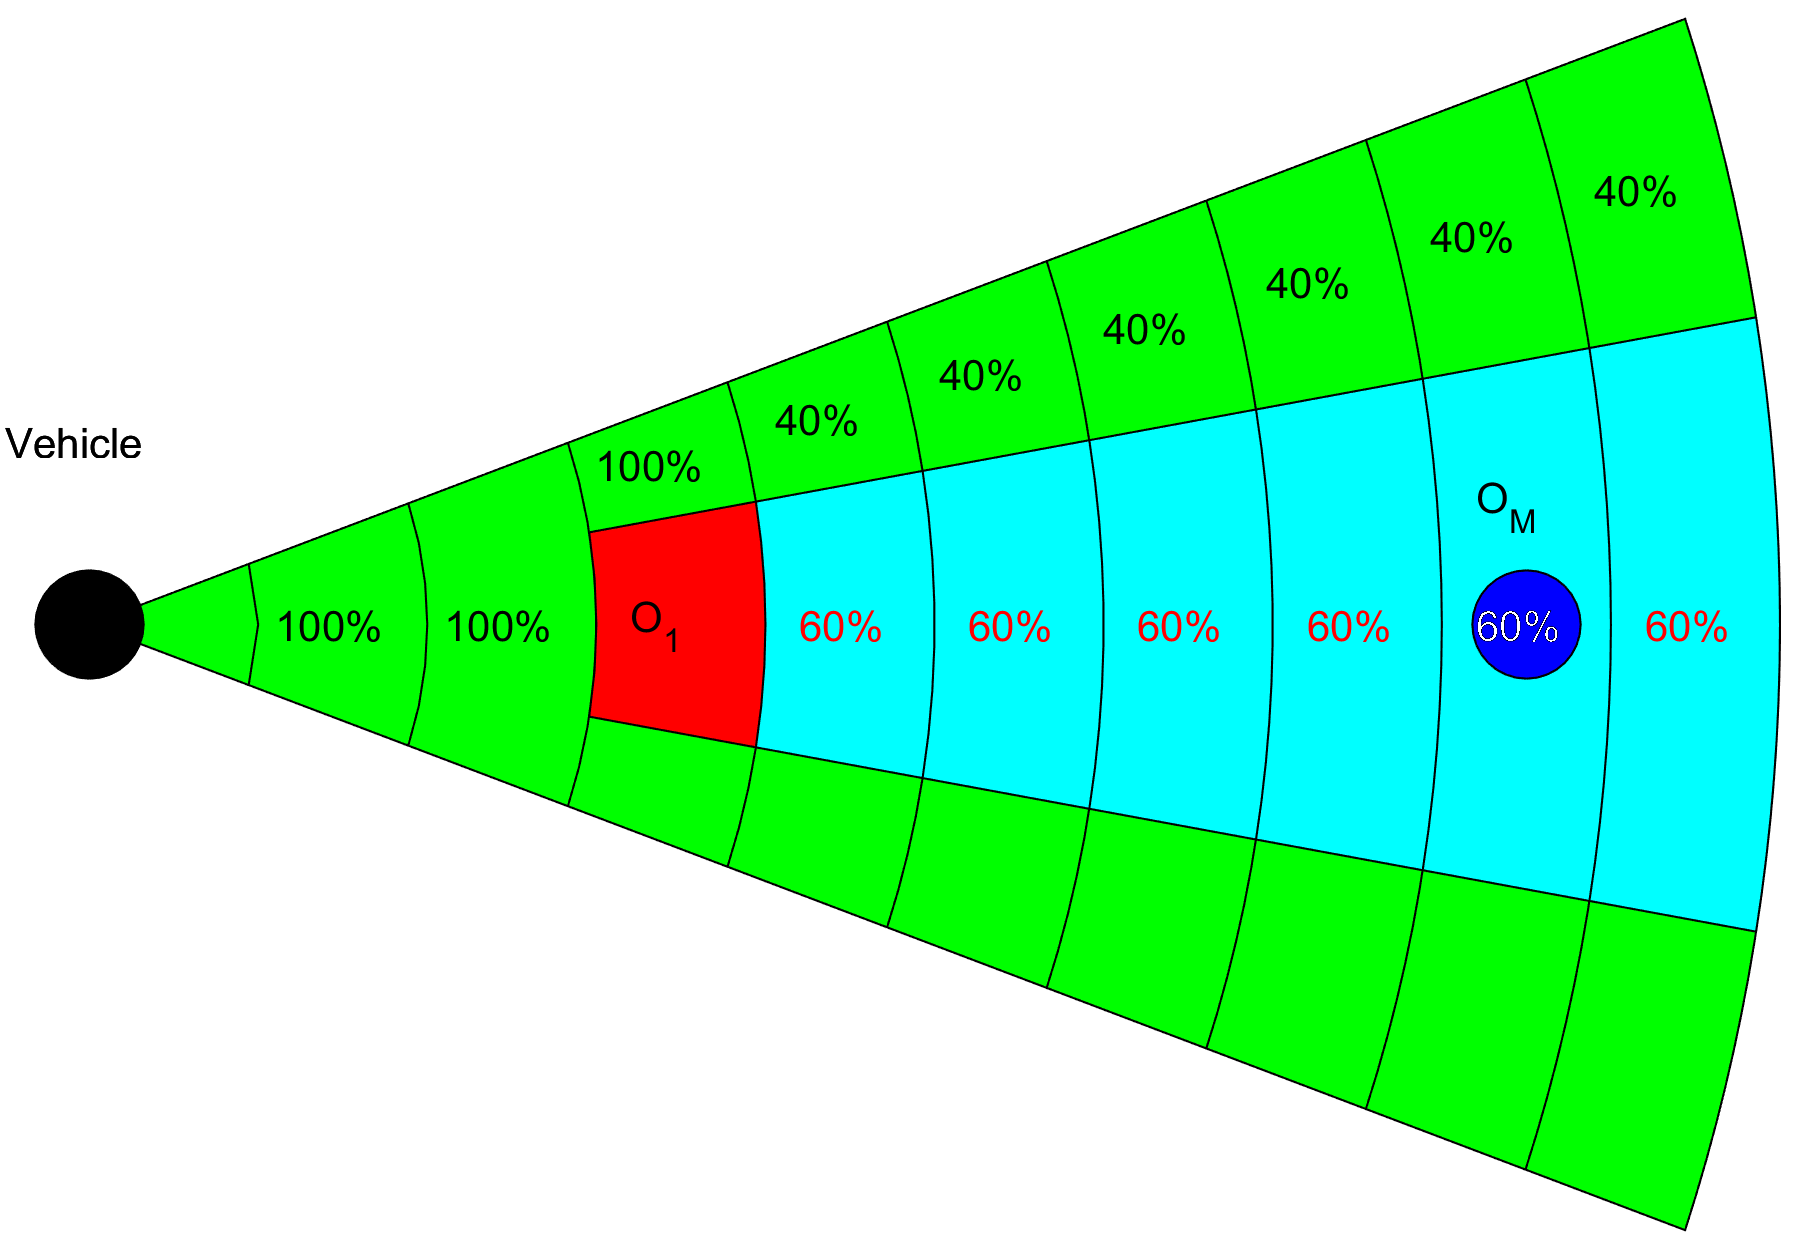
\includegraphics[width=0.9\linewidth]{\FIGDIR/TE011MapObstacleHiden}
        \caption{Hindered.}
        \label{fig:hinderedMapObstacle}
    \end{subfigure}
    \caption{Map obstacle states after \emph{Data fusion}.}
    \label{fig:mapObstacleStatesAfterDataFusion}
\end{figure}

\paragraph{Concept:} A \emph{map obstacle} state has very simple logic, there are three possible cases:

\begin{enumerate}
    \item \emph{Undetected} - Map obstacle $O_M$ is charted on map (fig. \ref{fig:undetectedMapObstalce}), but is undetected by any sensor in sensor field, therefore the probability of map obstacle occurrence is equal to $0$.


    \item \emph{Detected} Map obstacle $O_M$ is charted on map and detected by any sensor in sensor field (fig. \ref{fig:detectedMapObstacle}). The map obstacle rate is equal to detected obstacle rate, usually its equal to $1$.

    \item \emph{Hindered} Map obstacle $O_M$ is hindered behind other detected obstacle $O_1$ (fig. \ref{fig:hinderedMapObstacle}). The detected obstacle $O_1$ is in $cell_{i,j,k}$ and is reducing visibility in follow up $cellRow_{i_f>i,j,k}$ by $60$ percent.
\end{enumerate}

\paragraph{Implementation:} The formulation of final map obstacle rate  $map(cell_{i,j,k})$ was outlined in previous examples. These examples are showing the \emph{desired behaviour} and its solved by \emph{data fusion} (sec. \ref{s:sensorFusion}).

First we start with obstacle map definition. The obstacle map  (eq. \ref{eq:obstacleMap}) defines an map obstacle set of information vectors with position in global coordinate frame , orientation bounded to global coordinate reference frame, safety margin and additional parameters.
\begin{equation}\label{eq:obstacleMap}
    obstacle Map= 
    \left\{
    \begin{bmatrix}
        position,\\
        orientation,\\
        safety Margin,\\
        parameters
    \end{bmatrix}
    :
    \begin{aligned}
        & position \in  \R^3(GCF),\\
        & orientation \in \R^3(GCF),\\
        & safety Margin \in \R^+(m),\\
        & parameters \in \{\dots\}
    \end{aligned}
    \right\}
\end{equation}


The \emph{Map Obstacle} concept is taken from my \emph{master student work} \cite{cernamaria2018}, implementing \emph{compact representation} of point-cloud obstacle map. Te example of \emph{cuboid obstacles} with \emph{safe zone} is given in (fig. \ref{fig:exampleExtractedMapObstacles}).
    
\begin{figure}[H]
    \centering
    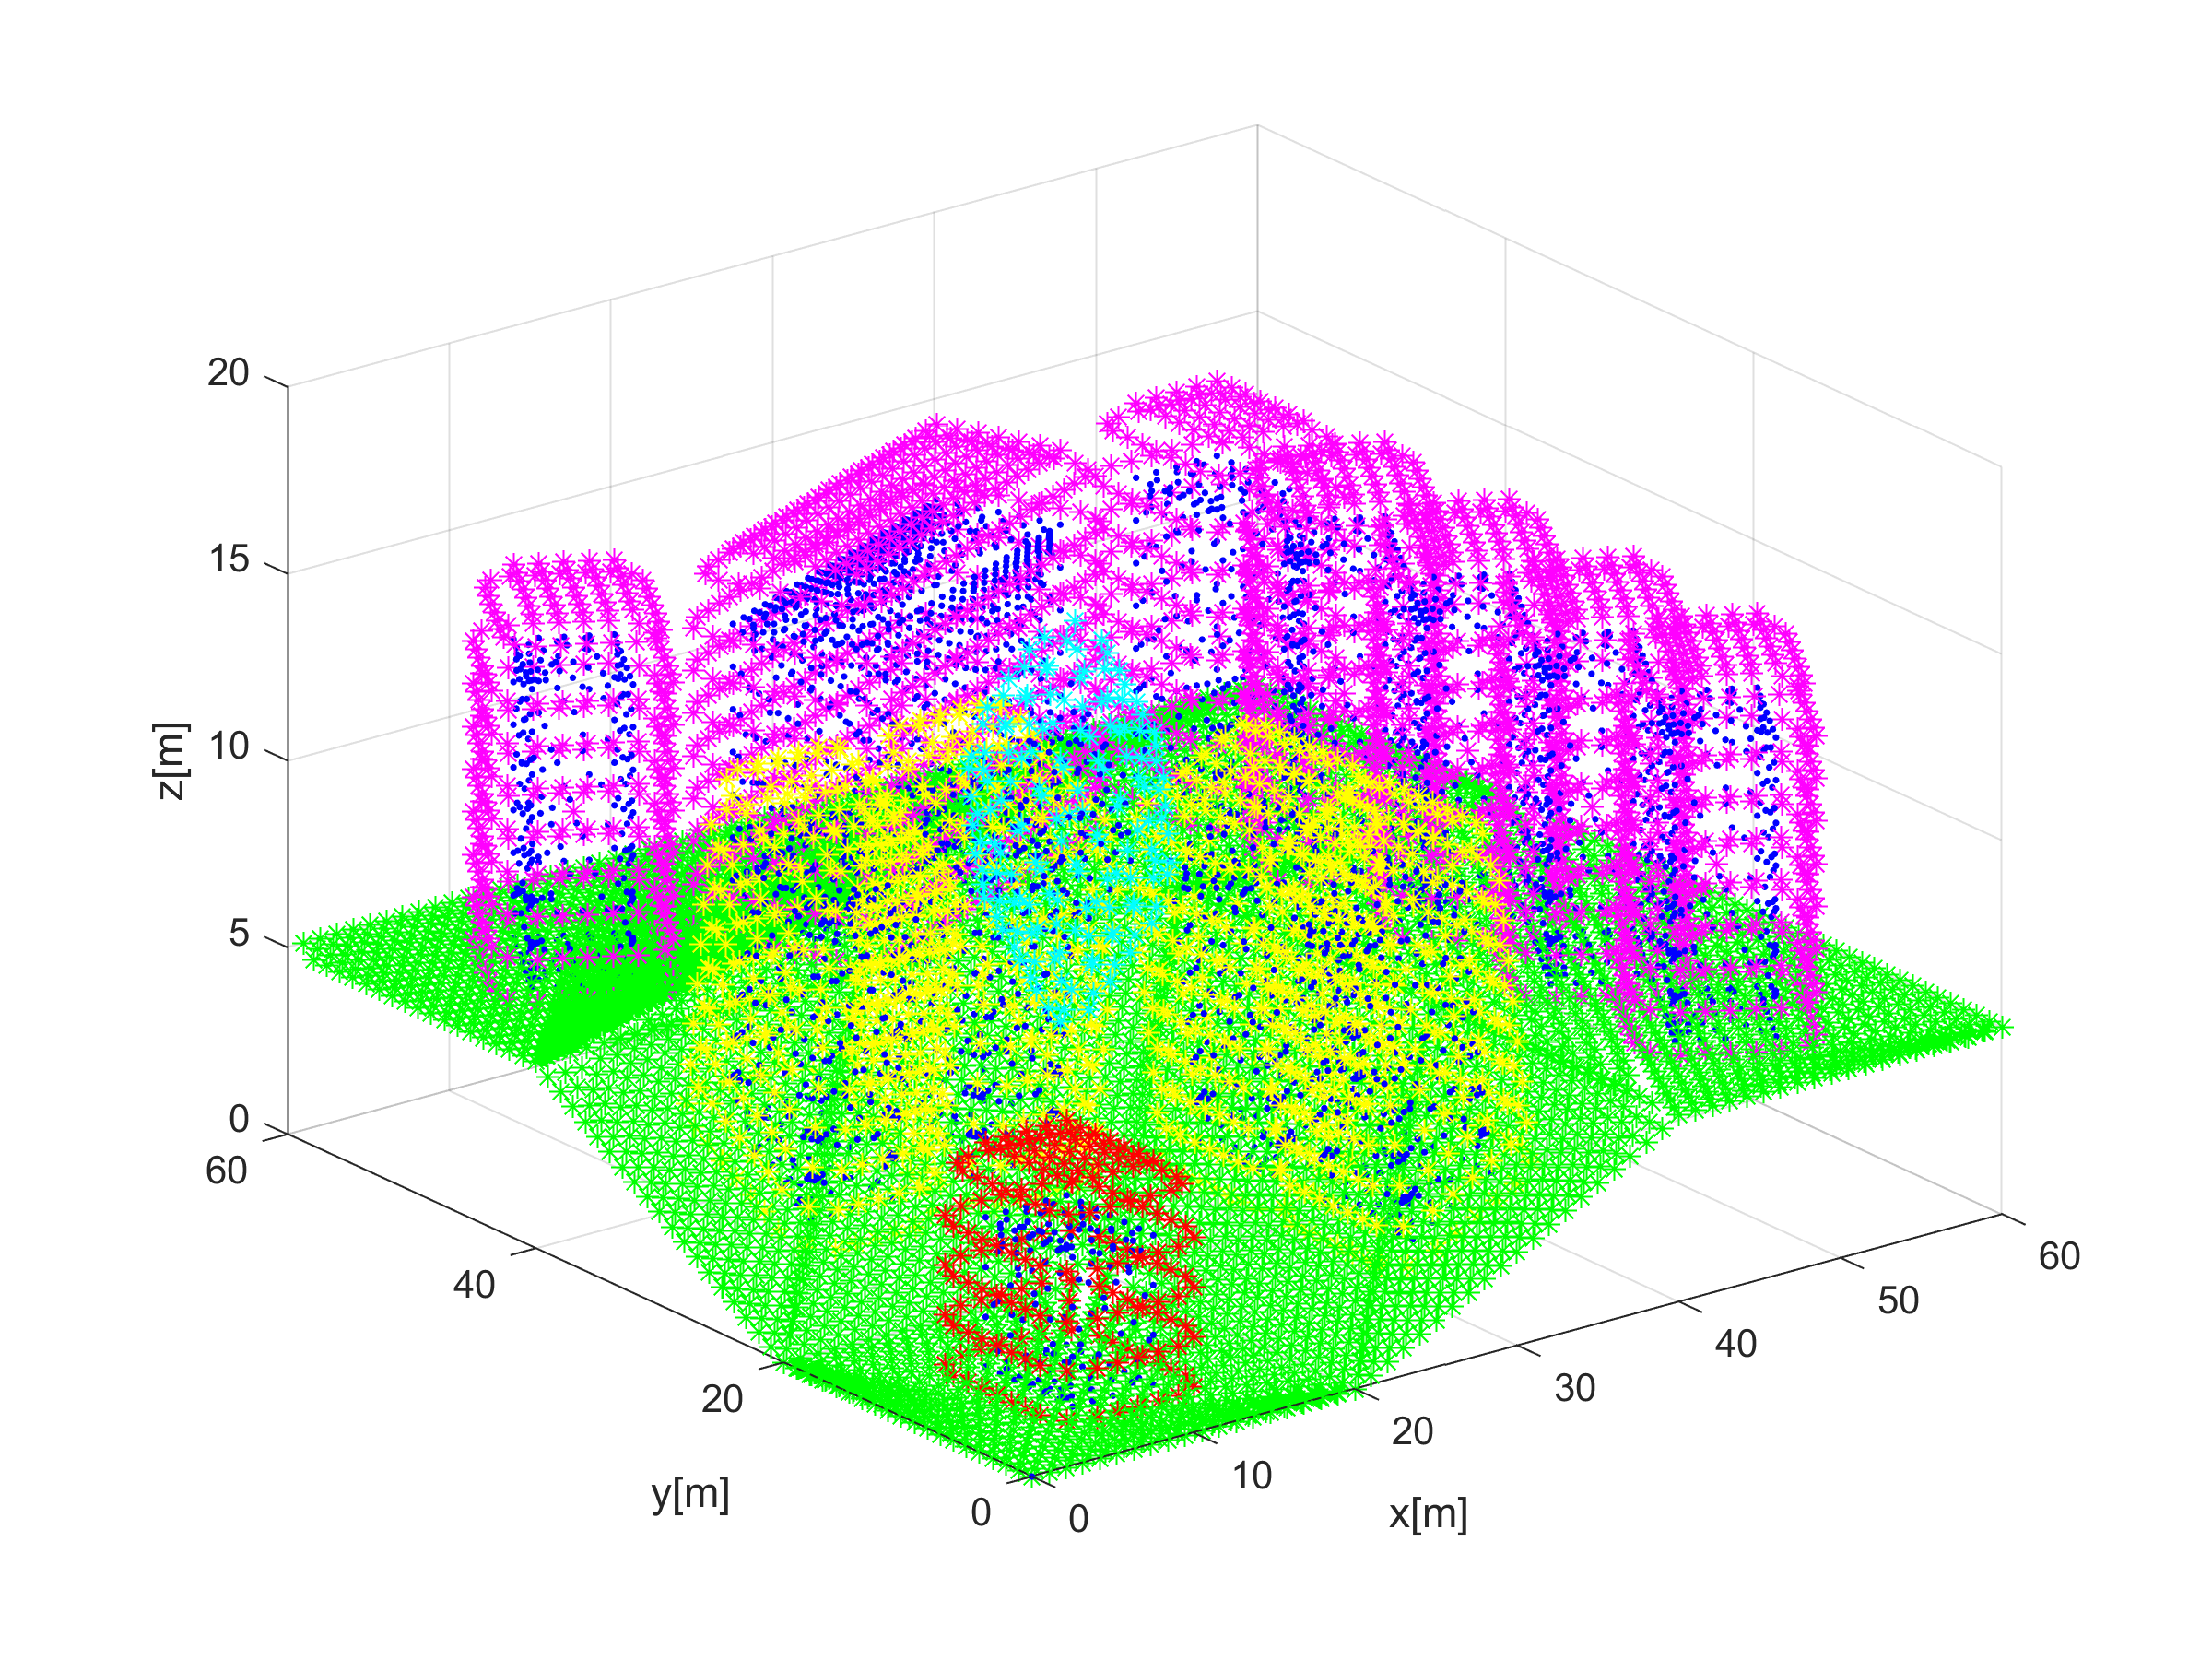
\includegraphics[width=0.7\textwidth]{\FIGDIR/TE054ExtractedMapObstaclesExample}
    \caption{Example of Extracted Map Obstacle \cite{cernamaria2018}.}
    \label{fig:exampleExtractedMapObstacles}
\end{figure} 

\noindent The space covered by any obstacle  is non-empty by definition. There are following types of map charted obstacles which are implemented in framework:

\begin{enumerate}
    \item\emph{Ball obstacle $parameters=\varnothing$} - simple ball with center at $position$, with offset safety margin.
    
    \item\emph{Line obstacle $parameters=[length]$} - simple line bounded by length $\in]0,\infty[$ with center at $position$ and given orientation with respect to main axis in global coordinate frame, with safety margin $<$ 0.
    
    \item\emph{Plane obstacle $parameters=[length,width]$} - bounded rectangle plane partition defined by length $\in]0,\infty[$, and width $w\in]0,\infty[$ with center at $\vec{p}$ and given orientation $\vec{o}$ with respect to main axis in global coordinate frame, with safety margin.
    
    \item\emph{Cuboid obstacle $parameters=[length,width,depth]$} - bounded cuboid space partition defined by length $\in]0,\infty[$, width $\in]0,\infty[$, and depth $d\in]0,\infty[$ with center at $position$ and rotated in orientation with respect to main axis in global coordinate frame, with safety margin.
\end{enumerate}

\noindent The \emph{map obstacles} are stored in clustered database. The \emph{selection criterion} is given in (eq. \ref{eq:mapObstacleSelectionCriterion}).

\begin{equation}\label{eq:mapObstacleSelectionCriterion}
    avoidance Grid.radius \ge distance(UAS.position,map Obstacle) - total Margin
\end{equation}

\noindent The \emph{total margin} is combination of \emph{safety margin} and \emph{body margin} (in case of line, plane, cuboid obstacle). The \emph{selection} was implemented as standard cluster select, selecting 26  surrounding clusters around UAS + own UAS cluster.

\noindent The \emph{compact obstacle representation} is transformed into \emph homogeneous point-cloud representations:

\begin{itemize}
    \item[1.]\emph{Body Point-cloud} - representing obstacle body approximation by geometrical shape (eq. \ref{eq:mapBodyPointCloud}). This point cloud is considered as hard constraints.
    
    \begin{equation}\label{eq:mapBodyPointCloud}
        body Point Cloud  =\{point\in\R^3(GCF): point \in map Obstacle Body\}
    \end{equation}
    
    \item[2.]\emph{Safety Margin Point Cloud} - representing safety coating around mapped obstacle body approximation (eq. \ref{eq:mapMarginPointCloud}). This point cloud is considered as soft constraint.
    \begin{equation}\label{eq:mapMarginPointCloud}
        margin Point Cloud = \{point\in\R^3(GCF): point \in map Safety Margin\}
    \end{equation}
\end{itemize}

\begin{note}
    The \emph{safety margin point cloud} is hollow in relationship to an \emph{body point cloud}, therefore:
    \begin{equation*}
        body Point Cloud \cap margin Point Cloud  = \varnothing
    \end{equation*}
\end{note}

\noindent The \emph{map obstacle} discretization to point cloud leads to problem how to calculate \emph{impact rate}. The \emph{theoretical impact rate} for \emph{obstacle} is given as:
\begin{equation*}
    impact Rate = \frac{volume(map Obstacle\cap cell_{i,j,k})}{volume(cell_{i,j,k})}\in [0,1]
\end{equation*}

\noindent The \emph{map obstacle related point clouds} (eq. \ref{eq:mapBodyPointCloud}, \ref{eq:mapMarginPointCloud}) are homogeneous \cite{cernamaria2018}. That means \emph{each point} in point clouds covers similar portion of object volume. There is \emph{threshold volume} (eq. \ref{eq:tresholdVolumeDefinition}) which represents minimal object volume to be considered as an \emph{obstacle}.

\begin{equation}\label{eq:tresholdVolumeDefinition}
    0< threshold Volume \le \frac{volume(point Cloud)}{|point Cloud|}
\end{equation}

\noindent The \emph{impact rate} of one point  when intersecting a $cell_{i,j,k}$ is given as count of \emph{threshold obstacle bodies} in \emph{point cloud covered mass} multiplied by inverted point count (eq. \ref{eq:pointImpactRateMap}).

\begin{equation}\label{eq:pointImpactRateMap}
    point. rate = \frac{point Cloud Volume}{threshold Volume}\times\frac{1}{|point Cloud|}
\end{equation}

The \emph{intersection set} between \emph{point cloud} and $cell_{i,j,k}$ is defined in (eq. \ref{eq:pointImpactRateMap}). The \emph{cell} intersection with points is defined in (eq. \ref{eq:boundedSpaceCell}).

\begin{multline}\label{eq:pointcloudIntersectionMap}
    intersection(map,cell_{i,j,k}) =\dots\\\dots \{points \in \R^3: (point\to Avoidance Grid Frame) \in cell_{i,j,k}\}
\end{multline}

\newpage \noindent The \emph{map obstacle rating} for $cell_{i,j,k}$ and obstacle for our \emph{information source} is defined in (eq. \ref{eq:mapcellratingourMap}).

\begin{equation}\label{eq:mapcellratingourMap}
    map(cell_{i,j,k},obstacle) =\max\left\{ \sum_{\forall point\in intersection(map,cell_{i,j,k})}  point.rate , 1\right\}
\end{equation}

\noindent The \emph{map obstacle rating} for $cell_{i,j,k}$ and \emph{our information source} is given as maximum of all possible cumulative ratings form each obstacle in \emph{active map obstacles} set (eq. \ref{eq:cumulativeMapCellRatingMap}).

\begin{equation}\label{eq:cumulativeMapCellRatingMap}
    map(cell_{i,j,k} = \max \left\{map(cell_{i,j,k},obstacle):\forall obstacle \in Active Map Obstacles\right\}
\end{equation}

\begin{note}
    The \emph{body point clouds} (eq. \ref{eq:mapBodyPointCloud}) never intersects, because they are created for inclusive obstacles. The \emph{safety margin point clouds} (eq. \ref{eq:mapMarginPointCloud}) can intersects, because they represents protection zones around physical obstacles. Therefore the \emph{maximum obstacle rating} (eq. \ref{eq:cumulativeMapCellRatingMap}) needs to be selected.
\end{note}

		\subsection{Constraints}\label{s:virtualConstraints}
\paragraph{Static Constraints:} The \emph{constraints} (ex. weather, airspace) usually covers a large portion of the \emph{operation airspace}. 

Converting constraints into valued \emph{point-cloud} is not feasible, due to the \emph{huge amount of created points} and low \emph{intersection rate}. The \emph{polygon intersection} or \emph{circular boundary of a 2D polygon} is a simple and effective solution \cite{ritter1990efficient,welzl1991smallest}. 

The key idea is to create \emph{constraint barrels} around dangerous areas. Each \emph{constraint barrel} is defined by a circle on the \emph{horizontal plane} and the \emph{vertical limit range}.

\paragraph{Representation:} The \emph{minimal representation} is based on (sec. \ref{sec:WellClear}, \ref{sec:WeatherImpact}) and geo-fencing principle. The \emph{horizontal-vertical separation} is ensured by \emph{projecting boundary} as 2D polygon oh horizontal plane and \emph{vertical boundary} (barrel height) as \emph{altitude limit}. 

The \emph{static constraint} (eq. \ref{eq:staticConstraint}) is defined as a structure vector including:
\begin{enumerate}
    \item \emph{Position} - the center position in the global coordinates\emph{2D horizontal plane}.
    
    \item \emph{Boundary} - the ordered set of boundary points forming edges in the global coordinates\emph{2D horizontal plane}.
    
    \item \emph{Altitude Range} - the \emph{barometric altitude} range $[altitude_{start},$ $altitude_{end}]$.
    
    \item \emph{Safety Margin} - the \emph{protection zone} (soft constraint) around constraint body (hard constraints) in meters.
\end{enumerate}

\begin{equation}\label{eq:staticConstraint}
    constraint = \{position,boundary, altitude_{start},altitude_{end}, safety Margin\}
\end{equation}

\paragraph{Active constrain selection:} The \emph{active constraints} are constraints which are impacting \emph{UAS active avoidance range}. 

The \emph{active constraints set} (eq. \ref{eq:activeConstraintSet}) is defined as a set of \emph{constraints} from all \emph{reliable Information Sources} where the \emph{distance} between UAS and constraint body (including safety margin) is lesser than the avoidance grid range. The \emph{horizontal altitude range} of avoidance grid must also intersect with \emph{constraint altitude range}.

\begin{multline}\label{eq:activeConstraintSet}
    Active Constraints = \dots\\\dots =
    \left\{\begin{aligned}constraint& \in Information Source:\\ 
    &distance(constraint,UAS) \le Avoidance Grid. distance,\\
    &constraint.altitude Range \cap UAS.altitude Range \neq \varnothing 
    \end{aligned}\right\}
\end{multline}

\paragraph{Cell Intersection:} The \emph{importance of constraints} is on their impact on \emph{avoidance grid} $cells$. The \emph{most of the constraints} (weather, ATC) are represented as 2D convex polygons. Even the \emph{irregularly shaped constraints} are usually split into smaller convex 2D polygons.

The idea is to represent convex polygon boundary as a sufficiently large circle to cover polygon. The Welzl algorithm to find \emph{minimal polygon cover circle} \cite{welzl1991smallest} is used.

First the \emph{set of contraint edges} (eq. \ref{eq:constraintEdgeSet}) is a enclosed set of 2D edges between neighboring points defined as follow:

\begin{equation}\label{eq:constraintEdgeSet}
    edges(constraint) =
    \left\{
    \begin{bmatrix}
        point_{i},point_{j}
    \end{bmatrix}:
    \begin{aligned}
    &point\in boundary,\\
    &i \in \{1,\dots,|boundary|\},\\
    &j \in \{2,\dots, |boundary|,1\}\\
    \end{aligned}
    \right\}
\end{equation}

\noindent The \emph{constraint circle boundary} with calculated center on the  2D horizontal plane and radius (representing body margin) is defined in (eq. \ref{eq:constraintCircleBoundary}).

\begin{equation}\label{eq:constraintCircleBoundary}
    circle(constraint)=
    \left[
        \begin{aligned}
            & center = \frac{\sum boundary.point}{|boundary.point|} + correction\\
            & radius = smallest Circle(edges(constraints)) 
        \end{aligned}
    \right]
\end{equation}

\noindent The $(cell_{i,j,k}$ and \emph{constraint} intersection (eq. \ref{eq:contraintToCellIntersection}) is classification function. The \emph{classification} is necessary, because one \emph{constraint} induce: 
\begin{enumerate}
    \item \emph{Body Constraint} (hard constraint) - the distance between $cell_{i,j,k}$ closest border and \emph{circular boundary} center is in interval $[0,radius]$.
    
    \item \emph{Protection Zone Constraint} (soft constraint) - the distance between $cell_{i,j,k}$ closest border and \emph{circular boundary} center is in interval $]radius,radius+safety Margin]$.
\end{enumerate}


\begin{multline}\label{eq:contraintToCellIntersection}
    intersection,constraint)=\dots\\\dots = 
    \begin{cases}
        hard &:\left[
            \begin{aligned}
                &distance(cell_{i,j,k},circle(constraint)) \le\dots\\ 
                &\quad\dots\le circle(constraint).radius,\\
                & constraint.altitude Range \cap cell_{i,j,k}.altitude Range \neq \varnothing,
            \end{aligned}\right]\\
             &\\
        soft &:\left[
            \begin{aligned}
                &distance(cell_{i,j,k},circle(constraint)) >\dots\\ 
                &\quad\dots > circle(constraint).radius,\\
                &distance(cell_{i,j,k},circle(constraint)) \le\dots\\ 
                &\quad\dots\le circle(constraint).radius + safety Margin,\\
                & constraint.altitude Range \cap cell_{i,j,k}.altitude Range \neq \varnothing,
            \end{aligned}\right]\\
             &\\
        none &:otherwise
    \end{cases}
\end{multline}

\noindent The \emph{intersection impact} of constraint is handled separately for \emph{soft} and  \emph{hard} constraints. The \emph{avoidance} of hard constraints is \emph{mandatory}, the \emph{avoidance} of soft constraints is \emph{voluntary}.

The constraints which have a \emph{soft intersection with the cell} are added to cells impacting constraints set: 
\begin{equation}\label{eq:softConstraintsCellIntersections}
    cell_{i,j,k}. soft Constraints = 
    \left\{
        \begin{aligned}
            &constraint \in Active Constraints:\\ 
            &\quad intersection(cell_{i,j,k},constraint) = soft
        \end{aligned}
    \right\}
\end{equation}

\noindent The constraints which have a \emph{hard intersection with the cell} are added to cells impacting constraints set:

\begin{equation}\label{eq:hardConstraintsCellIntersections}
    cell_{i,j,k}. hard Constraints = 
    \left\{
        \begin{aligned}
            &constraint \in Active Constraints:\\ 
            &\quad intersection(cell_{i,j,k},constraint) = hard
        \end{aligned}
    \right\}
\end{equation}

\begin{note}
    The final \emph{constraint rate value} (eq. \ref{eq:constraintRatingForCell}) is determined based on \emph{mission control run} feed to \emph{avoidance grid} (fig. \ref{fig:missionControlRunActivityDiagram}) defined in  7\textsuperscript{th} to the 10\textsuperscript{th} step.
\end{note}
    

		
	%06-05 Moving Obstacles and Intruders	
    \subsection{Intruders}\label{s:intruders}
\paragraph{Intruder behavior:} \emph{Adversarial behavior} of moving obstacle is trying to destroy avoiding our UAS.  The \emph{Intruder} UAS \cite{fiorini1998motion} is not trying to hurt our \emph{UAS} actively. The \emph{Adversarial behaviour} is neglected in this work. The non-cooperative avoidance is assumed, it can be relaxed to \emph{cooperative avoidance} in \emph{UTM controlled airspace}.

\paragraph{Intruder information:} The \emph{observable intruder information set} for any kind of intruder, obtained through the sensor/C2 line, is following:
\begin{enumerate}
    \item\emph{Position} - position of an intruder in the \emph{local} or \emph{global} coordinate frame, which can be transformed into \emph{avoidance grid coordinate frame}.
    
    \item\emph{Heading and Velocity} - intruder heading and linear velocity in avoidance grid coordinate frame.
    
    \item\emph{Horizontal/Vertical Maneuver Uncertainty Spreads} - how much can an \emph{intruder} deviate from the \emph{original linear path} in a \emph{horizontal/vertical} plane in \emph{Global coordinate Frame}.
\end{enumerate}

 

\begin{figure}[H]
    \centering
    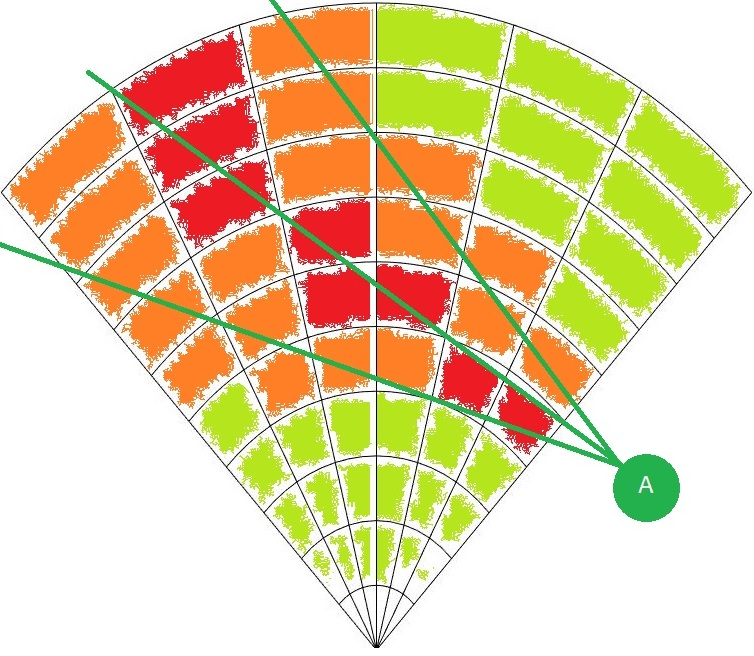
\includegraphics[width=0.7\textwidth]{\FIGDIR/TE052AdversaryProbabilitySpread}
    \caption{Intruder UAS intersection rate along the expected trajectory.}
    \label{fig:intruderProbabiltySpreadTheoretical}
\end{figure}   

\paragraph{Example of Intruder Intersection:} Let us neglect the \emph{time-impact} aspect on the \emph{intersection}.  The \emph{intruder} (black "I" circle) is intersecting one \emph{avoidance grid horizontal slice} (fig. \ref{fig:intruderProbabiltySpreadTheoretical}).  The intruder is moving along linear path approximation based on velocity (middle green line). The \emph{Horizontal Maneuver Uncertainty spread} is in \emph{green line boundary area} \emph{intruder intersection rating} is denoted as green-orange-red cell fill reflecting intersection severity:  red is a high rate of the intersection, orange is the medium rate of the intersection and green is a low rate of the intersection.
    


\paragraph{Moving Threats:} The \emph{UAS} can encounter following threats during the \emph{mission execution}:
\begin{enumerate}
    \item \emph{Non-cooperative Intruders} - the intruders who does not implement any approach to ensure mutual avoidance efficiency.
    
    \item \emph{Cooperative Intruders} - the intruders whom actively communicate or follow common agreed behavior pattern (ex. Rules of the Air).
    
    \item \emph{Moving Constraints} - the constrained portion of \emph{free} space which is shifting its boundary over time (ex. Short term bad weather).
\end{enumerate}
    
\begin{note}
    Our approach considers only \emph{UAS} intruders because \emph{Data Fusion} considers data received through \emph{ADS-B} messages. The \emph{Intruders} extracted from \emph{LiDAR} scan were not considered (ex. birds). The proposed \emph{intruder intersection models} are reusable for other \emph{intruder sources}.
\end{note}

\paragraph{Approach Overview:} The \emph{Avoidance Grid} (def. \ref{def:AvoidanceGrid}) is adapted to the \emph{LiDAR} sensor. The \emph{Euclidean grid intersections} are fairly simple. The \emph{polar coordinates grid} is not. The need to keep \emph{polar coordinates grid} is prevalent, because of fast \emph{LiDAR} reading assessment.  There are following commonly known methods to address this issue:

\begin{enumerate}
    \item\emph{Point-cloud Intersections} - the \emph{threat impact area} is discredited into a sufficiently thick point cloud. This point-cloud have \emph{point impact rate} and \emph{intersection time} assigned to each point. The \emph{point-cloud} is projected to \emph{Avoidance Grid}. If the \emph{impact point} hits $cell_{i,j,k}$ the cell`s impact rate is increased by the amount of \emph{point impact rate}. The final \emph{threat impact rate} in $cell_{i,j,k}$ is given when \emph{all} points from point cloud are consumed. Close point problem \cite{shamos1975closest} was solved by the application of method  \cite{bentley1980optimal}.
    
    \item\emph{Polygon Intersections} - the \emph{threat impact area} is modeled as a polygon, each $cell_{i,j,k}$ in \emph{Avoidance Grid} is considered as a \emph{polygon}. There is a possibility to calculate cell space geometrical inclusive intersection. The \emph{impact rate} is then given as rate between \emph{intersection volume} and $cell_{i,j,k}$ volume. The algorithm used for intersection selected based on:\citep{bentley1979algorithms} the selected algorithm  \emph{Shamos-Hoey} \cite{shamos1976geometric}.
\end{enumerate}

\begin{note}
    The \emph{Intruder Intersection} models are based on \emph{analytical geometry} for \emph{cones and ellipsoids} taken from \cite{sommerville2016analytical}.
\end{note}

    	\subsection{(R) Intruder Behaviour Prediction}\label{s:intruderBehaviourPrediction}
\paragraph{Idea:} \emph{Intruder Intersection Models} is about space-time intersection of \emph{intruder body} with \emph{avoidance Grid} and \emph{Reach Set}:
\begin{enumerate}
    \item The \emph{UAS} reach set defines \emph{time boundaries} to \emph{enter/leave} cell in avoidance grid.
    \item The \emph{Intruder} behavioral pattern defines \emph{rate} of \emph{space intersection} with cell bounded space in avoidance grid.
\end{enumerate}

The multiplication of \emph{space intersection rate} and \emph{time intersection rate} will give us \emph{intruder intersection} rate for our \emph{UAS} and intruder.


\paragraph{Intruder Dynamic Model:} The  definition of avoidance grid enforces the  most of these methods to be numeric. Let us introduce intruder dynamic model:

\begin{equation}\label{eq:intruderBasicLinearModel}
    \begin{aligned}
        \partial position /\partial time = velocity 
    \end{aligned}
    \quad | \quad
    \begin{aligned}
        position_x(t) = position_x(0) + velocity_x \times t\\
        position_y(t) = position_y(0) + velocity_y \times t\\
        position_z(t) = position_z(0) + velocity_z \times t
    \end{aligned}
\end{equation}

\noindent Position vector in euclidean coordinates $[x,y,z]$   is transformed into \emph{Avoidance Grid} coordinate frame. Velocity vector for $[x,y,z]$  is \emph{estimated and not changing}. The time  is in interval $[entry,leave]$, where $entry$ is intruder entry time into avoidance grid and $leave$ is intruder leave time from avoidance grid. 

\begin{note}
    If \emph{intruder} is considered, time of entry is marked as $intruder_{entry,k}$ where k is intruder identification, time of leave is marked as $intruder_{leave,k}$ where k is intruder identification. 
\end{note}

\paragraph{Cell Entry and Leave Times} $UAS_{entry}(cell_{i,j,k})$ and $UAS_{leave}(cell_{i,j,k})$ are depending on intersecting  \emph{Trajectories} and \emph{bounded cell space} (eq. \ref{eq:boundedSpaceCell}). There is \emph{Trajectory Intersection} function from (def. \ref{def:ContainedReducedReachSet}) which evaluates \emph{Trajectory segment} entry and leave time. 

The UAS \emph{Cell Entry} time is given as minimum of all \emph{passing trajectory segments} entry times (eq. \ref{eq:cellEntryTime}), if there is no \emph{passing trajectories} the UAS \emph{entry time} is set to 0.

\begin{equation}\label{eq:cellEntryTime}
    UAS_{entry}(cell_{i,j,k}) =  \min 
    \left\{\begin{aligned}
    0,en&try(Trajectory,cell_{i,j,k}):\\ &Trajectory\in Passing Trajectories
    \end{aligned}\right\}
\end{equation}

The UAS \emph{Cell Leave} time is given as maximum of all \emph{passing trajectory segments} entry times (eq. \ref{eq:cellLeaveTime}), if there is no \emph{passing trajectories} the UAS \emph{leave time} is set to 0.

\begin{equation}\label{eq:cellLeaveTime}
    UAS_{leave}(cell_{i,j,k}) =  \max 
    \left\{\begin{aligned}
    0,lea&ve(Trajectory,cell_{i,j,k}):\\ &Trajectory\in Passing Trajectories
    \end{aligned}\right\}
\end{equation}

\paragraph{Time Intersection Rate:} The key idea is to calculate how long the \emph{UAS} and \emph{Intruder} spends together in same space portion ($cell_{i,j,k}$). 
The \emph{Intruder} can spent some time in $cell_{i,j,k}$ bounded by interval of \emph{intruder} entry/leave time. 

The \emph{UAS} can spent some time, depending on \emph{selected trajectory} from \emph{Reach Set}. The time spent by UAS is bounded by entry (eq. \ref{eq:cellEntryTime}) and leave (eq. \ref{eq:cellLeaveTime}). 

The intersection duration of these two intervals creates \emph{time intersection rate} numerator, the \emph{maximal duration} of \emph{UAS} stay gives us \emph{denominator}. The \emph{time intersection rate} is formally defined in (eq. \ref{eq:timeIntersectionRate}). 

\begin{equation}\label{eq:timeIntersectionRate}
    time\left(\begin{gathered}UAS,\\Intruder,\\cell_{i,j,k}=\circ\end{gathered}\right)=  
    \frac{
        \left|
        \begin{gathered}
            \ [intruder_{entry}(\circ),intruder_{leave}(\circ)] \\
            \cap\\
            [UAS_{entry}(\circ),UAS_{leave}(\circ)]
        \end{gathered}\right|
        }
        {
        \left|\left[UAS_{entry}(\circ),UAS_{leave}(cell_{\circ})\right]\right|
        }
\end{equation}


\paragraph{Intruder Intersection Rate:} The \emph{Intruder Intersection Rate} (eq. \ref{eq:intruderIntersectionProbability}) is calculated as \emph{multiplication} of \emph{space intersection rate} (defined later) and \emph{time intersection rate} (eq. \ref{eq:timeIntersectionRate}).

\begin{equation}\label{eq:intruderIntersectionProbability}
    intruder\left(\begin{gathered}UAS,\\Intruder,\\cell_{i,j,k}\end{gathered}\right) = time \left(\begin{gathered}UAS,\\Intruder,\\cell_{i,j,k}\end{gathered}\right) \times space\left(\begin{gathered}UAS,\\Intruder,\\cell_{i,j,k}\end{gathered}\right)
\end{equation}

\begin{note}
    If there is no information to derive \emph{Intruder} entry/leave time for cells the \emph{time intersection rate} is considered 1.
\end{note}

The \emph{Intruder cell reach} time (eq. \ref{eq:intruderIntersectionTimeonPoint}) is bounded to discrete point in intersection model \cite{shamos1975closest,bentley1980optimal}. The intruder \emph{entry/leave time} is calculated similar to \emph{UAS cell entry (eq. \ref{eq:cellEntryTime})/leave (eq. \ref{eq:cellLeaveTime}) time}.

\begin{equation}\label{eq:intruderIntersectionTimeonPoint}
    point Reach Time(Intruder,point) = \frac{distance(Intruder.initial Position, point)}{|Intruder.velocity}
\end{equation}


\paragraph{Space Intersection Rate:} The \emph{Space Intersection Rate} reflects probability of \emph{Intruder} intersection with portion of space bounded by $cell_{i,j,k}$, to be precise with intruder trajectory or vehicle body shifted along the trajectory. The principles for \emph{space intersection rate} calculation are following:




\begin{enumerate}
    \item \textit{Line trajectory} - \emph{intruder} trajectory is given by linear approximation (eq. \ref{eq:intruderBasicLinearModel}), depending on \emph{intruder size} the intersection with avoidance grid can be:
    
    \begin{enumerate}[a.]
        \item \emph{Simple line} - intersection is going along the trajectory line line defined by intruder model (eq.\ref{eq:intruderBasicLinearModel}).
    
        \item \emph{Volume line} - intersection is going along the trajectory line defined by intruder model (eq. \ref{eq:intruderBasicLinearModel}) and intruder`s \emph{body radius} is considered in intersection.
    \end{enumerate}
    
    \item \emph{Elliptic cone} - initial position is considered as the top of a cone, the main cone axis is defined by intruder linear trajectory (eq. \ref{eq:intruderBasicLinearModel}) $time \in [0,\infty]$. The cone width is set by horizontal and vertical spread.
\end{enumerate}

    	\subsection{(R) Linear Intersection}\label{s:linearIntersectionModel}
\paragraph{Idea:} There are \emph{small intruders} which have body \emph{smaller} than average $cell_{i,j,k}$ cell size. Its trajectory will stick to \emph{linear trajectory} prediction with high probability. 

\paragraph{Space Intersection Rate:} The \emph{Space Intersection Rate} for $cell_{i,j,k}$ is implemented as simple point cloud intersection. Where \emph{sufficiently thick} point cloud is defined along \emph{line} (eq. \ref{eq:linearModelIntruderLineIntersection}):

\begin{equation}\label{eq:linearModelIntruderLineIntersection}
    position(time) = position(time_0) + velocity \times time,\quad time \in [0,\infty[
\end{equation}

Then there exist projection function from local euclidean coordinates to local polar coordinates (eq. \ref{eq:projecionFunctionplanarEuclidlinearIntersection}. The function projects intruder trajectory (eq. \ref{eq:linearModelIntruderLineIntersection}) to planar coordinates $[distance,$ $horizontal^\circ,$ $vertical^\circ]$  as a set of sufficiently thick point cloud.

\begin{equation}\label{eq:projecionFunctionplanarEuclidlinearIntersection}
    polarSet:position(t)\to\{[distance, horizontal^\circ], vertical^\circ\}
\end{equation}


\noindent The \emph{space intersection rating} $SpaceIntersection(\circ)$ for line type is given as (eq. \ref{eq:baseIntersectionProbabilityLineIntersectionType}). If there exist non empty intersection of $polarSet\cap cell_{i,j,k}$ there is space intersection rate equal to  1, if intersection $polarSet\cap cell_{i,j,k} = \varnothing$ then the rate is zero.

\begin{equation}\label{eq:baseIntersectionProbabilityLineIntersectionType}
    space\left(\begin{gathered}Intruder,\\cell_{i,j,k}\end{gathered}\right)=
    \begin{cases}
        1:&\exists point \in polarSet(eq.\ref{eq:projecionFunctionplanarEuclidlinearIntersection}): point \in c_{i,j,k}\\
        0:&\text{otherwise}
    \end{cases}
\end{equation}

\begin{note}
    The \emph{intruder intersection rate} is multiplication of \emph{space intersection rate} and time intersection rate. The \emph{intersection rate} is calculated for \emph{every intruder} and \emph{selected intersection model} separately.
\end{note}

    	\subsection{(R) Body-volume Intersection}\label{s:bodyvolumeIntersection}
\paragraph{Idea:} The \emph{Intruder} has \empty body volume greater than \emph{average} $cell_{i,j,k}$ volume. The \emph{intruder body} is considered as the ball moving along \emph{intruder position}. The \emph{intersection} of the intruder body is realized as sufficiently thick \emph{point-cloud intersection}.

\paragraph{Space Intersection Rate - Body Volume:} The \emph{body volume mass} with center at $position(t)$ is moving along intruder trajectory prediction (eq. \ref{eq:linearintersectionmodelVehicleVolume}) in time interval $[0,\infty[$:

\begin{equation}\label{eq:linearintersectionmodelVehicleVolume}
    position(time) = position(time_0) + velocity \times time
\end{equation}

\noindent The body \emph{Volume ball} $Body(position(t),radius)$ (eq. \ref{eq:volumeballofIntruder}) is defined as set of points in $\R^3$ euclidean space. The center is moving along the \emph{position(t)}. The body \emph{volume ball} is a set of points sufficiently thick including also inner points. The \emph{thickness} is guaranteed by existence of neighbour point which is close enough.

\begin{equation}\label{eq:volumeballofIntruder}
    Body(position(t),radius) = \left\{point \in \R^3:\begin{aligned}&\norm{position(t) - point} \le radius\\ &\forall point_i \exists point_{j\neq i},\\ &distance(point_i,point_j)\le thickness\end{aligned} \right\}
\end{equation}

\noindent The \emph{polar volume ball} $polarBody$ (eq. \ref{eq:plannarCoordinateTransformationVolumeBall}) is projection of body volume ball  set $Body(position(t),radius)$ to a set of planar coordinates in avoidance grid coordinate frame:

\begin{equation}\label{eq:plannarCoordinateTransformationVolumeBall}
    polarBall(t):  Body(position(t),radius) \to \left\{\left[\begin{aligned}&distance, horizontal^\circ,\\ &vertical^\circ, intersection Time\end{aligned}\right]\right\}
\end{equation}

\newpage\noindent The \emph{space intersection rate for vehicle body} $space(Intruder, cell_{i,j,k})$ (eq. \ref{eq:baseIntersectionProbabilityBallIntersectionType}) is calculated as intersection of polar body volume ball and $cell_{i,j,k}$. If intersection is non empty then base probability is one, zero otherwise:

\begin{equation}\label{eq:baseIntersectionProbabilityBallIntersectionType}
    space\left(\begin{gathered}Intruder,\\cell_{i,j,k}\end{gathered}\right)=
    \begin{cases}
        1:&\exists point \in polarBall(eq.\ref{eq:plannarCoordinateTransformationVolumeBall}): point \in c_{i,j,k}\\
        0:&\text{otherwise}
    \end{cases}
\end{equation}

\paragraph{Intersection Time:} The \emph{intersection time} id depending on point cloud (eq. \ref{eq:plannarCoordinateTransformationVolumeBall}) where each point \emph{have intersection time} given as \emph{body-center position} time (eq. \ref{eq:linearintersectionmodelVehicleVolume}). 

\begin{note}
    The \emph{body-volume} intersection model, can insert the \emph{multiple intersection times} into one $cell_{i,j,k}$. the \emph{interval length} considers all of these for intersection rates (eq. \ref{eq:timeIntersectionRate}).
\end{note}
    

    	\newpage
\section{Maneuverability Uncertainty Intersection}\label{s:uncertaintyIntersection}
\paragraph{Idea:} The \emph{intruders} are not bullets they are not sticking to predicted linear paths. The \emph{intruder} maneuverability is given as horizontal and vertical spread. Therefore \emph{intruder reach set} will form an \emph{elliptic cone}. This cone can be transformed into \emph{finite discrete } point-cloud, each \emph{point} should have assigned \emph{severity} impact value.  The point cloud intersection with  \emph{Avoidance Grid} will give us space impact of an\emph{uncertain} intruder.


\begin{note}
    The following section will use condensed notation, due to the equation complexity. The \emph{terminology} is consistent with the rest of the section. 
\end{note}

\paragraph{Space Intersection Rate - Body Volume Intersection:} $P_T(i_k({x}_s,{v},\theta,\varphi),c_{i,j,k})$
computation is less straight-forward than other space intersection rates. First let us define the linear intruder $i_k$ positions ${x}$ at time $t$ (eq. \ref{eq:vehiclelinearcone}) model, where ${x}(t)$ defines intruder position in \emph{avoidance grid euclidean coordinate frame} at time $t_i$, ${v}$ defines intruder velocity, and $t$ is a time offset.

\begin{equation}\label{eq:vehiclelinearcone}
    x(t)=x_s + v_I.t
\end{equation}

\noindent Intruder \emph{horizontal spread} $\theta$ and \emph{vertical spread} $\varphi$ are introduced. These spreads represents intruder deviation limits along from linear trajectory prediction ${x}(t)\in\R^3$. The example is given by (fig. \ref{fig:P21ElipticConeIOnePoint}) where the intruder starts at point ${x}_s$ with fixed velocity $v$, the linear trajectory prediction is outlined by blue line. The \emph{predicted intruder position} at time $t=10s$ is given by ${x}(10)$ (blue point). The ellipsoidal space $E({x})$ is projected on the plane $D({x}(t))$. The plane $D$ (eq. \ref{eq:elisioidalOtrthogonalPlane}) for point ${x}(t)$ and velocity ${v}$ is defined as an orthogonal plane to velocity vector ${v}\in\R^3$ with origin at intruder position ${x}(t)$. 

\begin{equation}\label{eq:elisioidalOtrthogonalPlane}
    D({x}(t),{v})=\left\{{a}\in\R^3:({a}-{x}(t))\perp{v},\right\}
\end{equation}

To construct  ellipsoidal space boundary on orthogonal plane $D({x}(t),{v})$ some parameters are defined in (eq. \ref{eq:elipsiodialBoudaryParameters}). The \emph{scalar distance} $d_d{{x}(t)}$ is simple Euclidean norm, \emph{maximal horizontal offset} $d_\theta({x}_t)$ is given as product of sinus of horizontal offset angle $\theta$ and scalar distance $d_d$, and \emph{maximal vertical offset} $d_\varphi({x}(t))$ is given a product of sinus of vertical offset angle $\varphi$ and scalar distance $d_d$.

\begin{equation}\label{eq:elipsiodialBoudaryParameters}
    \begin{aligned}
     d_d                      &=d_d({x}(t),{x}_s) =\norm{{x}(t)-{x}_s}_2\\ 
     d_{\theta_{\text{max}}}  &= d_\theta({x}(t))=\sin\theta   (i_k).d_d({x}(t))\\
     d_{\varphi_{\text{max}}} &= d_\varphi({x}(t))=\sin\varphi (i_k).d_d({x}(t)) 
    \end{aligned}
\end{equation}


\noindent The \emph{Ellipsoid} $E({x}(t),{v})$ (eq. \ref{eq:baseElipsoidxt}) for fixed intruder position ${x}(t)$ and fixed intruder velocity ${v}$ is given as constrained portion of orthogonal plane $D({x}(t),{v})$. The constraint is defined by an internal coordinate frame ${p}\in \R^2$ which is space reduction of plane $D({x}(t),{v})$. 


\begin{figure}[H]
    \centering
    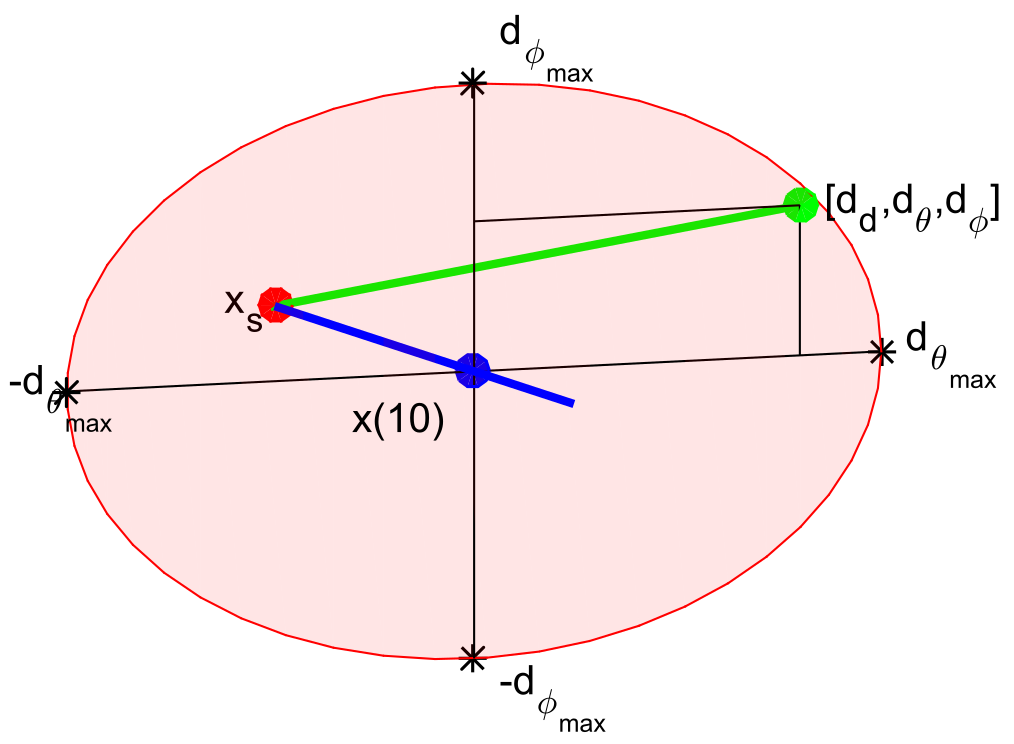
\includegraphics[width=0.7\textwidth]{\FIGDIR/TE014ElipticConeIOnePoint}         
    \caption{One rate position $[d_d,d_\theta,d_\varphi]$ (green). deviated from linear trajectory (blue line) at point ${x}(10)$.(blue) with initial position $x_s$ (red)}
    \label{fig:P21ElipticConeIOnePoint}
\end{figure}


The internal coordinate frame ${p}\in\R^2$ has origin in ${x}(t)\to\R^2$. The points of plane ${p}$ are bounded by projection ${p}=({b}-{x}(t))\to\R^2$, where $b\in D({x}(t),v)$. The point of ellipsoidal ${p}$ is then given as standard ellipse boundary with vertical span $d_\theta({x}(t))$ and horizontal span $d_\varphi({x}(t))$. 

The 2D \emph{Ellipsoid} $E({x}(t),{v})$ for specific time $t=10s$ example is portrayed  as red ellipsoid (in fig. \ref{fig:P21ElipticConeIOnePoint}).

\begin{equation}\label{eq:baseElipsoidxt}
    E({x}(t),{v})=\left\{ \begin{aligned}{b}\in\R^3:&{b}\in D({x}(t),{v}),{p}=({b}-{x}(t))\to\R^2,\\&\left(\frac{p(1)^2} {d_\theta({x}(t))^2}+ \frac{p(2)^2}{d_\varphi({x}(t))^2}\right)\le 1\end{aligned}\right\}
\end{equation}

\noindent The expected behavior of an intruder $i_k$ is to stick to predicted linear trajectory ${x}(t)$ (\ref{eq:vehiclelinearcone}). The probability of deviation should be decreasing with distance from the ellipse center (fig. \ref{fig:intruderPassingProbability}.).  


\noindent \emph{Probability density function} for ellipsoid  $E({x}(t),{v})$defined in (eq. \ref{eq:baseElipsoidxt}) is depending on maximal horizontal spread $d_\theta({x}(t))$, maximal vertical spread $d_\varphi({x}(t))$, defined by (eq. \ref{eq:elipsiodialBoudaryParameters}). 

Two standard probabilistic distributions are established $\mathscr{N}(\mu_\theta,\sigma_\theta)$ (eq. \ref{eq:elipsprobdistHorizontal}) for horizontal spread $\theta({x}(t))$ and $\mathscr{N}(\mu_\varphi,\sigma_\varphi)$  (eq. \ref{eq:elipsprobdistVertical}) for vertical spread $\varphi({x}(t))$. The means $\mu_\theta$ and $\mu_\varphi$ are set to zero, and internal coordinate frame ${p}\in\R^2$ where ${x}(t)\to\R^2$ is frame center. The variances $\sigma_\theta$ and $\sigma_\varphi$ are set as maximal distances on horizontal/vertical spread axes $d_\theta({x}(t))$ and $d_\varphi({x}(t))$.

\begin{equation}\label{eq:elipsprobdistHorizontal}
    P({x}(t),d_\theta)=\mathscr{N}(\mu_\theta,\sigma_\theta)=\mathscr{N}(0,d_\theta({x}(t)))
\end{equation}

\begin{equation}\label{eq:elipsprobdistVertical}
    P({x}(t),d_\varphi)=\mathscr{N}(\mu_\varphi,\sigma_\varphi)=\mathscr{N}(0,d_\varphi({x}(t)))
\end{equation}

\noindent The combined \emph{probability density function} for maximal spreads $d_\theta$ and $d_\varphi$ is given by (eq. \ref{eq:elipsprobdistCombined}). Because probability density function is defined for internal space ${p}\in\R^2$ and one may need to calculate impact rate for  cell space $c_{i,j,k}\in\R^3$. 

The reduction from two parameter probability distribution function to scalar rate distribution function is needed. A scalar rate distribution  function $P({x}(t),d_\theta,d_\varphi)$ over ellipsoid $E({x}(t),{v})$ is defined as (eq.\ref{eq:elipsprobdistCombined}), where the final rate is given as an average of two partial probabilities. 

Final space intersection rate $P({x}(t),d_\theta,d_\varphi)$ needs to be normalized to hold \emph{normal distribution condition} (eq. \ref{eq:normalDistrobitionCondition}). Normal distribution condition value (eq. \ref{eq:normalDistrobitionCondition}) is given as surface integral over ellipsoid $E({x}(0),{v})$ with rate distribution function $P({x}(t),d_\theta,d_\varphi)$.

\begin{equation}\label{eq:elipsprobdistCombined}
    P({x}(t),d_\theta,d_\varphi) = \frac{\mathscr{N}(\mu_\theta,\sigma_\theta)+\mathscr{N}(\mu_\varphi,\sigma_\varphi)}{2}
\end{equation}

\begin{equation}\label{eq:normalDistrobitionCondition}
    \iint_{E({x}(\tau))} P({x}(t),d_\theta,d_\varphi) \,\text{d}d_\theta\,\text{d}d_\varphi = 1
\end{equation}

\noindent Final space intersection rate  $P({x}(t),c_{i,j,k},\theta,\varphi)$  (space portion, time portion is calculated in (eq.\ref{eq:intruderIntersectionProbability}) is given by (eq. \ref{eq:spreadIntruderIntersectionProb}). Its mean value of all intersection rates $P({x}(\tau),c_{i,j,k},\theta,\varphi)$ where $\tau\in[i_e(c_{i,j,k}),i_l(c_{i,j,k})]$ is fixed point in intersection time interval.

An $P({x}(\tau),c_{i,j,k},\theta,\varphi)$ (\ref{eq:spreadIntersectionProbFixedtau}) is integration of rate density function $P({x}(\tau),d_\theta,d_\varphi)$ (eq. \ref{eq:elipsprobdistCombined}) in surface $E({x}(\tau),{v})$ to cell $c_{i,j,k}$ volume intersection. 

\begin{figure}[H]
    \centering
    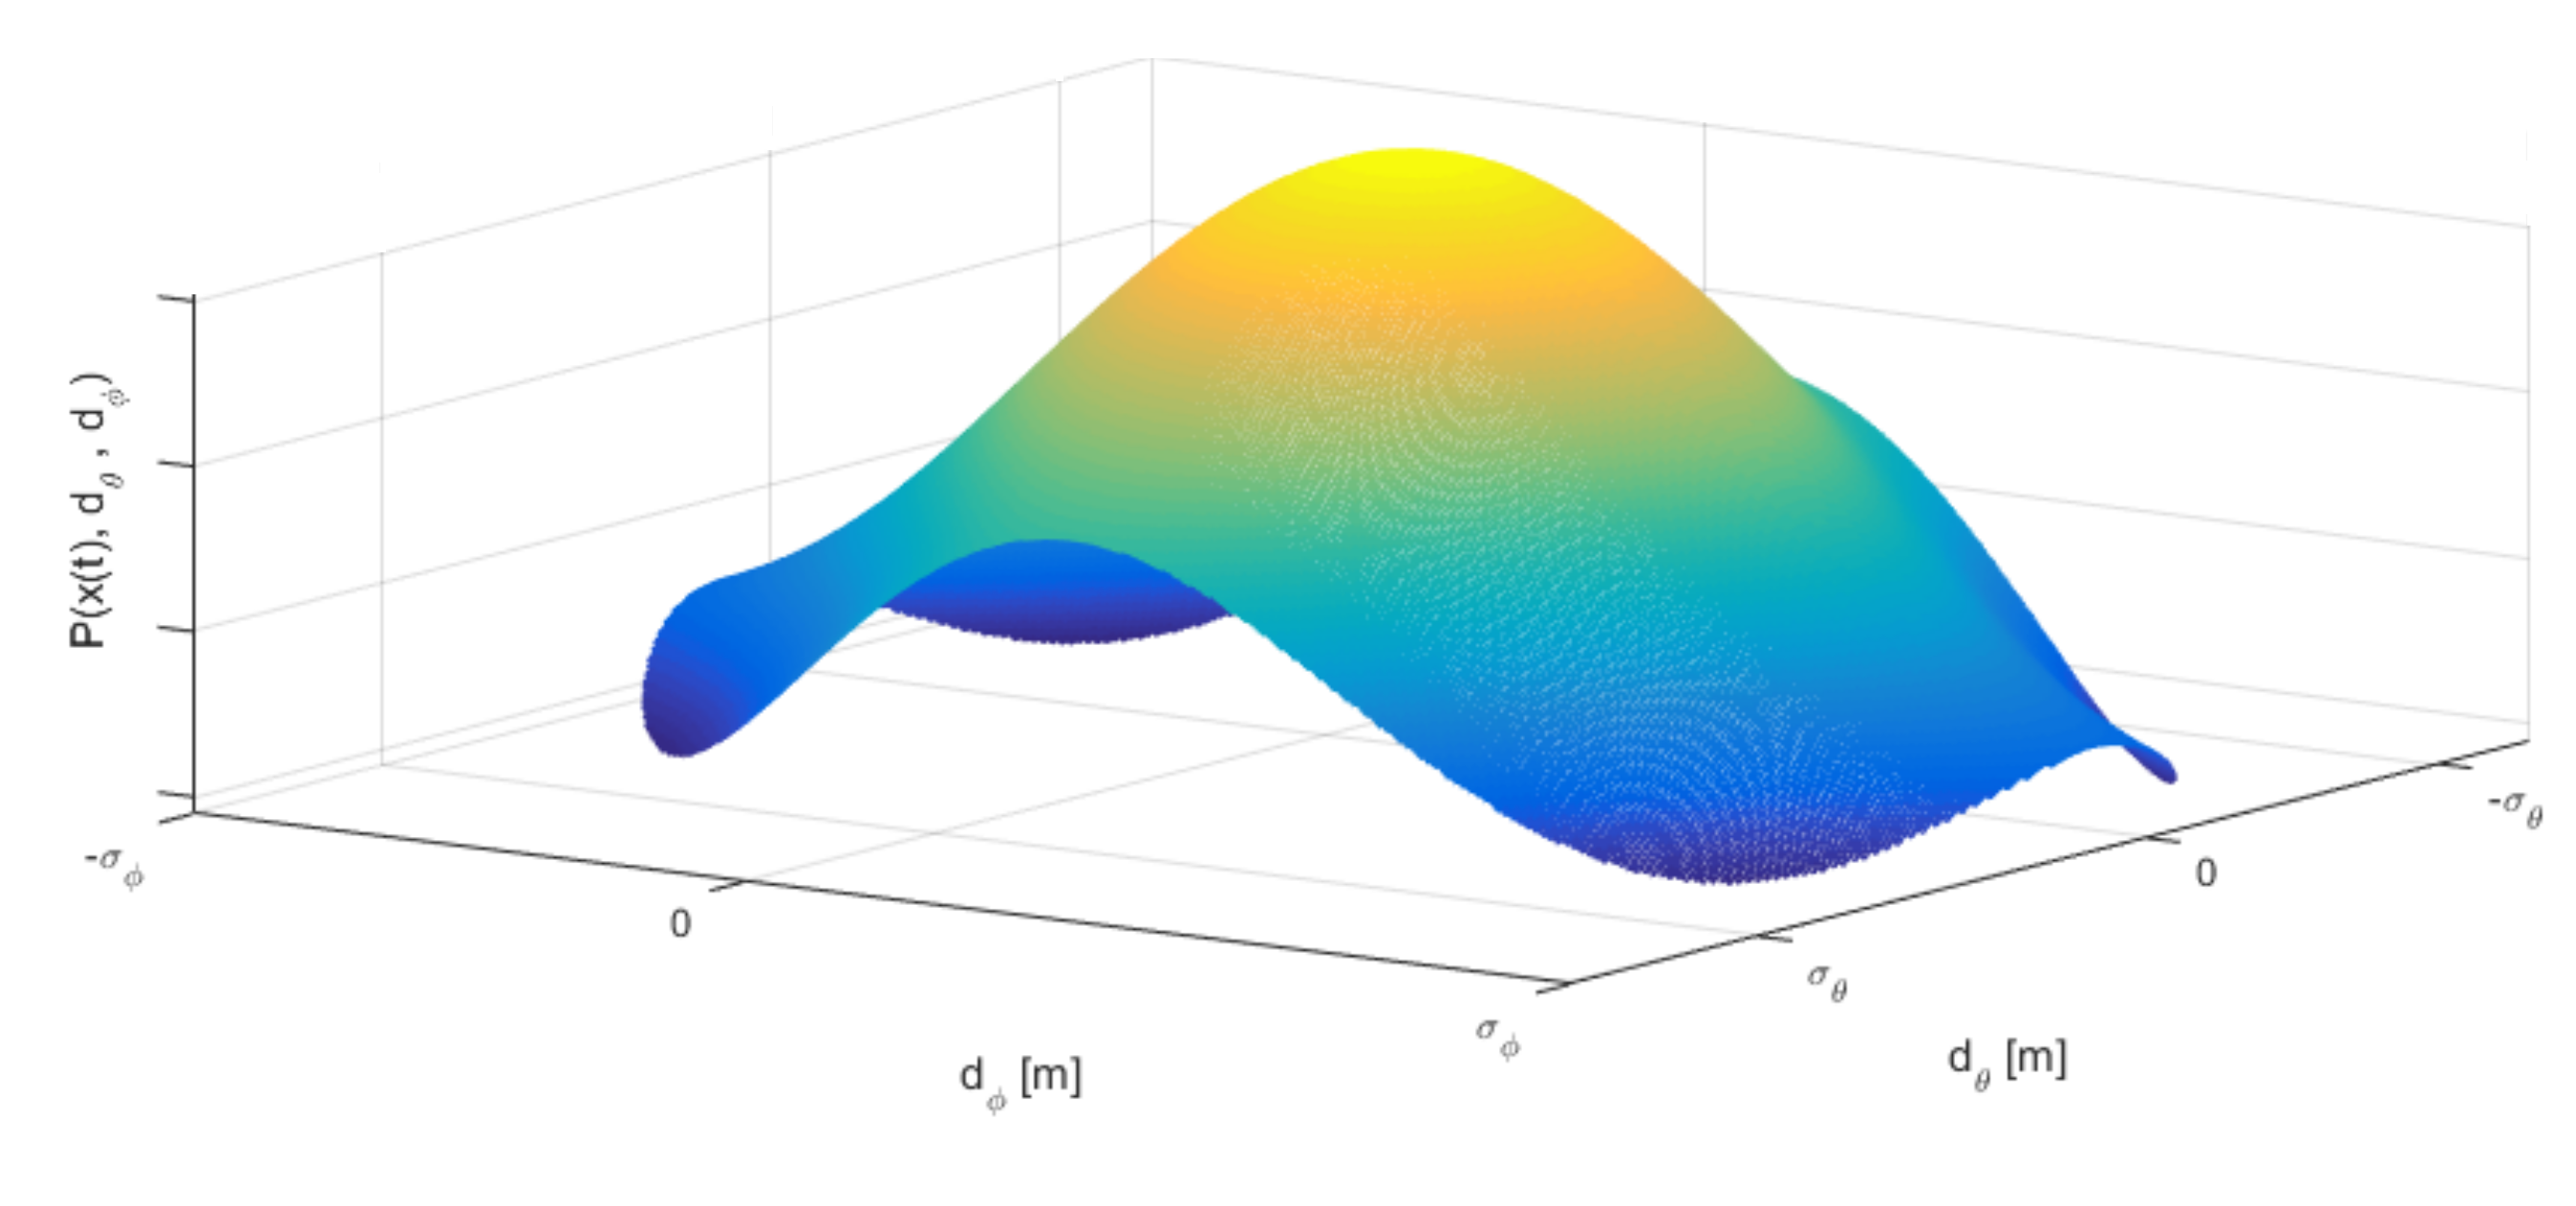
\includegraphics[width=0.9\textwidth]{\FIGDIR/TE015ProbabilisticDistributionOfEllipsoidCutSideForTE016}
    \caption{Probability of intruder $i_k$ position in ellipsoid $E({x}(t),{v})$}
    \label{fig:intruderPassingProbability}
\end{figure}

\noindent To get a volume integration partial rate in surface intersection must be integrated and normalized in time interval $\tau\in[i_e(c_{i,j,k}),i_l(c_{i,j,k})]$, the \emph{base intersection probability} $P_T(i_k({x}_s,{v},\theta,\varphi),c_{i,j,k})$ is given by (eq. \ref{eq:spreadIntruderIntersectionProb}). Example of intersection of intruder $i_r$ uncertain ellipsoid cone with avoidance grid $\mathscr{A}(t_i)$ is given in (fig. \ref{fig:ellipticConeIntersectionExample}).

\begin{equation}\label{eq:spreadIntersectionProbFixedtau}
    P({x}(\tau),c_{i,j,k},\theta,\varphi) =\iint_{E({x}(\tau),{v})\cap c_{i,j,k}} P({x}(\tau),d_\theta,d_\varphi)
\end{equation}

\begin{equation}\label{eq:spreadIntruderIntersectionProb}
    P_T(i_k({x}_s,{v},\theta,\varphi),c_{i,j,k})=\frac{\int_{i_e(c_{i,j,k})}^{i_l(c_{i,j,k})} P({x}(\tau),c_{i,j,k},\theta,\varphi)\,\text{d}\tau}{i_l(c_{i,j,k})-i_e(c_{i,j,k})}
\end{equation}

\begin{figure}[H]
    \centering
    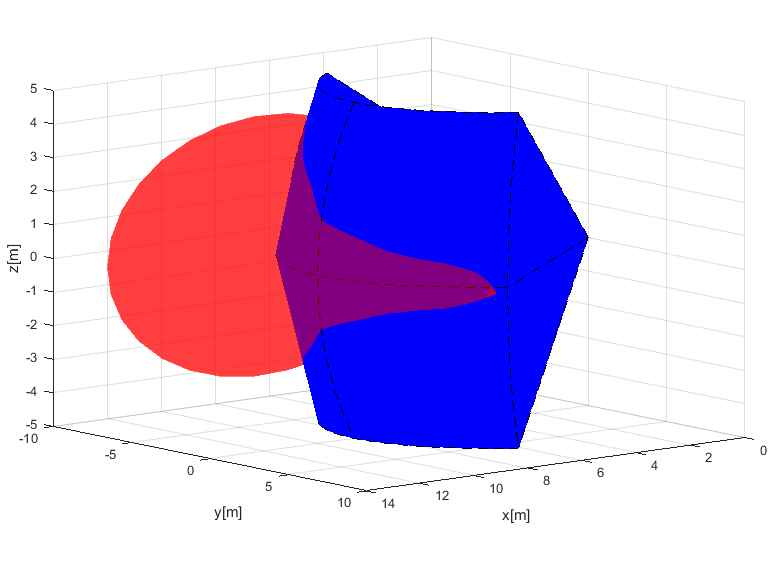
\includegraphics[width=0.7\textwidth]{\FIGDIR/TE013ElipticConeIntersecitonExample}
    \caption{Avoidance grid $\mathscr{A}(t_i)$ (blue) intersection with elliptic cone intruder $i_k({x},{v},\theta,\varphi)$ (red) example.}
    \label{fig:ellipticConeIntersectionExample}
\end{figure}

\noindent A \emph{numeric approximation} of space intersection rate $P_T(i_k({x}_s,{v},\theta,\varphi),c_{i,j,k})$ is more implementation feasible than symbolic calculation due to the multiple intersection constraints and bad intersection algorithm complexity. 

Let us define a homogeneous discrete subset of real numbers $\mathscr{R}$ which is a non-empty subset of real numbers $\R$. The set $\mathscr{R}$ (eq. \ref{eq:homogeneusdiscretizationofRealnumbers}) is homogeneous that means for an equal interval $(i,i+1],i\in\mathbb{Z}$ subset the count of members is equal to some positive natural number $k$. The parameter $k$ can be understood as \emph{unit approximation density}.

Similarly, the power sets $\mathscr{R}^2\subset\R^2$, $\mathscr{R}^3\subset\R^3$, ... $\mathscr{R}^i\subset\R^i,i\in\N^+$ keeps homogeneous distribution.

\begin{equation}\label{eq:homogeneusdiscretizationofRealnumbers}
    \mathscr{R} = \left\{\begin{aligned}a\in\R:&\forall i\in\mathbb{Z},|i<a\le i+1|=k,k\in\N^+, \\&\forall j\in \N^+a_{j+1}-a_{j}=m,m\in\R^+\end{aligned}\right\},\,\mathscr{R}\subset\mathbb{R}
\end{equation}

\noindent The orthogonal plane for ${x}(t), {v}, t \in\R$ is defined by (eq. \ref{eq:elisioidalOtrthogonalPlane}). The orthogonality property is also kept for any subspace $\mathscr{R}^n\in\R^n,n\in\N^+$. Numeric approximation of $D({x}(t),{v})$ is given as $D_D({x}(t),{v})$ (eq. \ref{eq:elisioidalOtrthogonalPlaneDiscrete}). 

The only difference is that discrete approximation is countable $|D_D|=m,m\in\N^+$, but continuous representation $|D|\approx \infty$ is uncountable. Because ellipsoid is a subset of orthogonal plane it keeps its countability property; therefore $E_D$ is also countable and must contain at least one member.

\begin{equation}\label{eq:elisioidalOtrthogonalPlaneDiscrete}
    D_D({x}(t),{v})=\left\{{a}\in\mathscr{R}^3:({a}-{x}(t))\perp{v},\right\},t\in\mathscr{R}
\end{equation}

\noindent The \emph{base ellipsoid} $E({x}(t),{v})$ for continuous-space is given by (eq. \ref{eq:baseElipsoidxt}). Every element, expect the base of internal projection $\mathscr{R}^2$ and orthogonal plane $D_D$ is same in discrete case $E_D({x}(t),{v})$ (eq. \ref{eq:baseElipsoidxtDiscrete}).

\begin{equation}\label{eq:baseElipsoidxtDiscrete}
    \bar{E}_D({x}(t),{v})=\left\{ \begin{aligned}{b}\in\mathscr{R}^3:&{b}\in D_D({x}(t),{v}),{p}=({b}-{x}(t))\to\mathscr{R}^2,\\&\left(\frac{p(1)^2} {d_\theta({x}(t))^2}+ \frac{p(2)^2}{d_\varphi({x}(t))^2}\right)\le 1\end{aligned}\right\},t\in\mathscr{R}
\end{equation}

\noindent The \emph{numeric calculation disproportion} can occur in case that ellipsoid $\bar{E}_D({x}(t),{v})$ (\ref{eq:baseElipsoidxtDiscrete}) in case of $d_\theta({x}(t))\approx 0$ and $d_\varphi({x}(t))\approx 0$. The count of ellipsoid members can be $|\bar{E}_D({x}(t),{v})|=0$, which is in contradiction with assumption $|\bar{E}_D({x}(t),{v})|\neq 0$. 

Let assume for discrete times $\tau=\left\{t_1,t_2,\dots,t_i\right\}$, $i\in \N^+$ there exists ellipsoids $\bar{E}_D({x}(t_1),{v})$,$\bar{E}_D({x}(t_1),{v})$, $\dots$, $\bar{E}_D({x}(t_i),{v})$ which are non empty and in space $\mathscr{R}^2$ in internal coordinate frame and space $\mathscr{R}^3$ in avoidance grid $\mathscr{A}(t_i)$ coordinate frame. The intersection of these partial ellipsoids in both spaces is equal to:

\begin{equation}
    \bar{E}_D({x}(t_1),{v})\cap \bar{E}_D({x}(t_2),{v})\dots\cap\dots \bar{E}_D({x}(t_i),{v}) = \varnothing
\end{equation}

\noindent An \emph{empty intersection} enables us to keep homogeneity property of ellipsoids by adding points so it is safe to add specific point ${x}(t)$ into empty ellipsoid. But only one, because it does not impact  probability density functions $\mathscr{N}(\mu_\theta,\sigma_\theta)$ and $\mathscr{N}(\mu_\varphi,\sigma_\varphi)$, neither space intersection rate  density function $P({x},d_\theta,d_\varphi)$. 

The final ellipsoid used forward $E_D({x}(t),{v})$(eq. \ref{eq:baseElipsoidxtDiscreteSafe}) is keeping all properties of ellipsoid $E({x}(t),{v})$ (eq. \ref{eq:baseElipsoidxtDiscreteSafe}). 

\begin{equation}\label{eq:baseElipsoidxtDiscreteSafe}
    E_D({x}(t),{v})= 
    \begin{cases}
        |\bar{E}_D({x}(t),{v})|=0 &: \left\{{x}(t)\right\} \\
        |\bar{E}_D({x}(t),{v})|\ge0 &: \bar{E}_D({x}(t),{v}) 
    \end{cases}
\end{equation}

\noindent The normal distribution condition for rate distribution function $P_D({x}(t),d_\theta,d_\varphi,{p})$, which is instance of to rate density function $P({x}(y),d_\theta,d_\varphi)$ (eq. \ref{eq:elipsprobdistCombined}) is used. This rate distribution must be normalized according to (eq.  \ref{eq:normalDistrobitionConditionDiscrete}).

\begin{equation}\label{eq:normalDistrobitionConditionDiscrete}
    \sum_{{p} \in E_D({x}(t))} P_D({x}(t),d_\theta,d_\varphi,{p}) = 1,\forall t\in\mathscr{R}^+
\end{equation}

\noindent The equations for \emph{space intersection rate} are similar to (eq. \ref{eq:spreadIntersectionProbFixedtau}, \ref{eq:spreadIntruderIntersectionProb}). For cell $c_{i,j,k}$ there exist intruder entry time $i_e(c_{i,j,k})$ its the earliest intersection with ellipsoid $E_D({x}(i_e(c_{i,j,k}))),{v}$. Same situation occurs with intruder leave time $i_l(c_i,j,k)$. Because $E_D$ is countable set, it means additional attributes can be attached to each point ${p}\in E_D$. Based on system dynamic (eq. \ref{eq:intruderBasicLinearModel}) the \emph{Time Of Arrival} (TOA) can be calculated. The example of TOA is given in fig. \ref{fig:intruderTimeOfArrival}.

\begin{figure}[H]
    \centering
    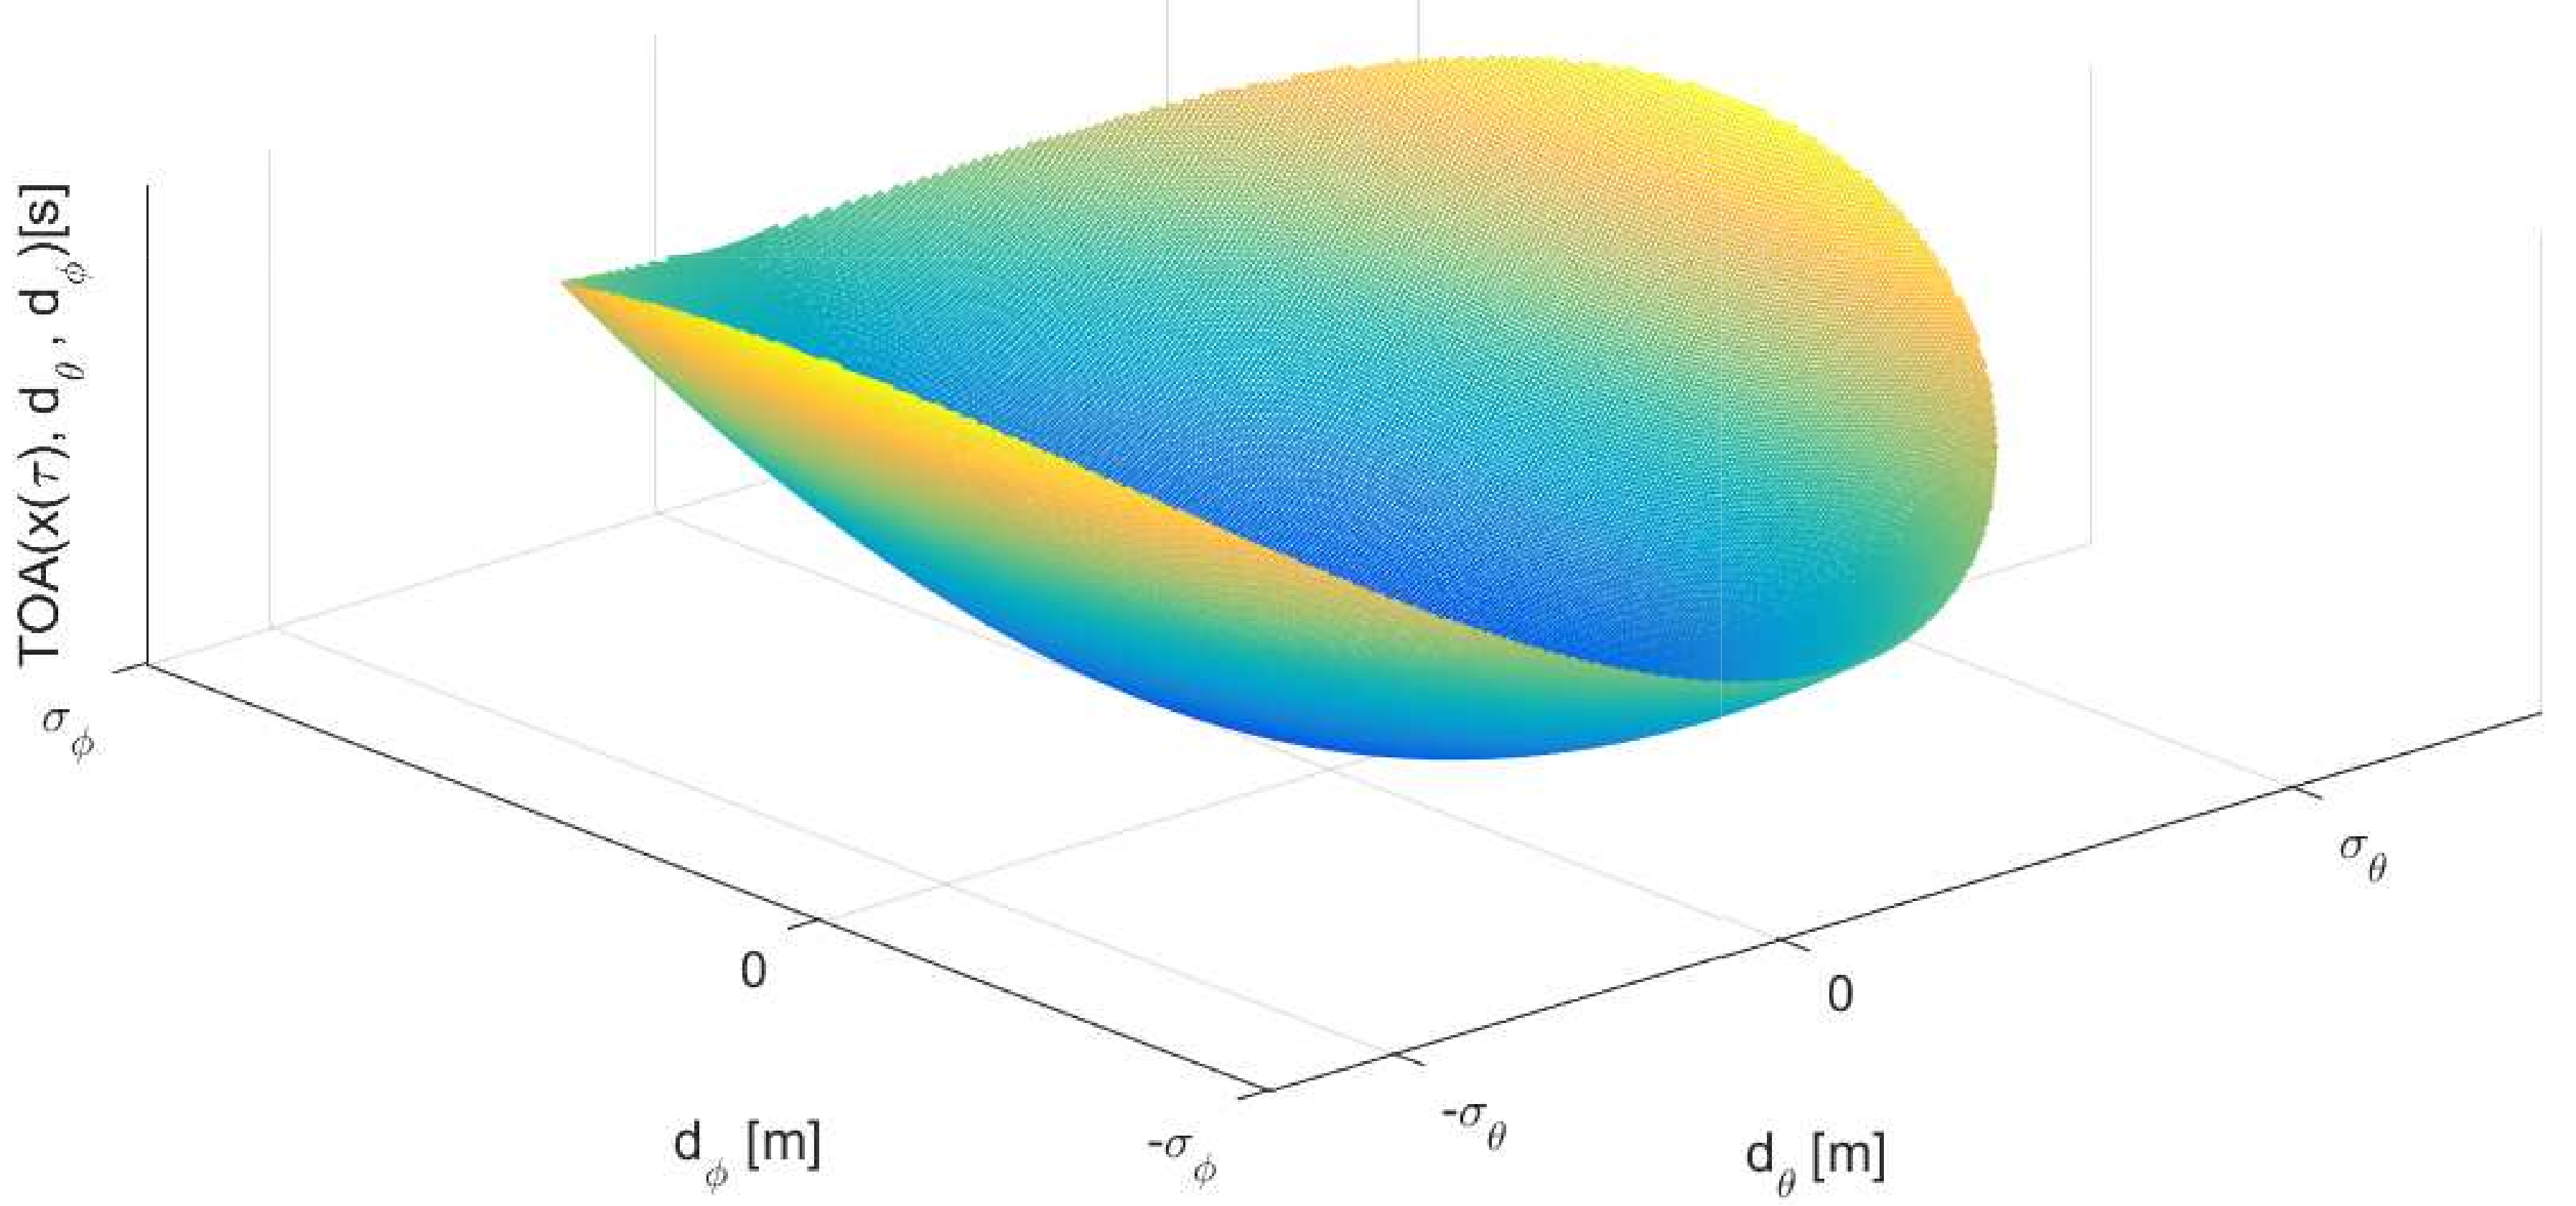
\includegraphics[width=0.7\textwidth]{\FIGDIR/TE016EllipsoidCutTimeOfArrival} 
    \caption{Time Of Arrival (TOA) for one ellipsoid $E_D({x}(\tau),{v})$.}
    \label{fig:intruderTimeOfArrival}
\end{figure}

\noindent The intersection rate $P_D({x}(\tau),c_{i,j,k},\theta,\varphi)$ for one time sample $\tau$ is given by (eq. \ref{eq:spreadIntersectionProbFixedtauDiscrete}), which has similar notation to (eq. \ref{eq:spreadIntersectionProbFixedtau}), sums are used instead of integrals and discrete rate density function $P_D({x}(\tau),d_\theta,d_\varphi,{p})$ for points form ellipse and cell intersection are used as iterator base set ${p}\in\left\{E_D({x}(\tau),{v})\cap c_{i,j,k}\right\}$.

\begin{equation}\label{eq:spreadIntersectionProbFixedtauDiscrete}
    P_D({x}(\tau),c_{i,j,k},\theta,\varphi) =\sum_{{p}\in \left\{E_D({x}(\tau),{v})\cap c_{i,j,k}\right\}} P_D({x}(\tau),d_\theta,d_\varphi,{p})
\end{equation}

\noindent The \emph{space intersection rate} $P_{TD}(i_k({x}_s,{v},\theta,\varphi),c_{i,j,k})$ (eq. \ref{eq:spreadIntruderIntersectionProbDiscrete}) is given as mean intersection rate of partial intersections $P_D({x}(\tau),c_{i,j,k},\theta,\varphi)$ where step set $T=\{$ $i_e(c_{i,j,k})$, $\dots$, $i_l(c_{i,j,k})\}$ contains all viable intersection times with ellipsoids $E({x}(\tau\in T),{v})$. The denominator is basically count of samples in sample time set $T$. 

\begin{equation}\label{eq:spreadIntruderIntersectionProbDiscrete} 
    P_{TD}(i_k({x}_s,{v},\theta,\varphi),c_{i,j,k})=\frac{\sum_{\tau=i_e(c_{i,j,k})}^{i_l(c_{i,j,k})} \sum_{{p}\in E_D({x}(\tau),{v})}P_D({x}(\tau),c_{i,j,k},\theta,\varphi,{p})}{\sum_{\tau i_l(c_{i,j,k})}^{i_e(c_{i,j,k})} 1}
\end{equation}

\noindent An \emph{intersection of intruder cone and cell} $c_{i,j,k}$ cell is defined by (eq. \ref{eq:conicIntersectionCellIntruderDiscrete}) The  set of point ${p}\in\mathscr{R}^3$ where condition of intersection between ellipsoids $E_D({x}(\tau),{v})$ for times $\tau\in\mathscr{R}^+$ and cell space $c_{i,j,k}$ is met.

\begin{equation}\label{eq:conicIntersectionCellIntruderDiscrete}
    \mathscr{P}(i_k({x}_s,{v},\theta,\varphi),c_{i,j,k})= \bigcup_{\forall \tau\in\mathscr{R}^+} \left\{{p}\in\mathscr{R}^3:{p}\in c_{i,j,k}\cap E_D({x}(\tau),{v})\right\}
\end{equation}

\noindent An \emph{intruder time of entry} $i_e(i_k,c_{i,j,k})$ (eq. \ref{eq:conicTimeOfEntryDiscrete}), for intruder $i,k$ and cell $c_{i,j,k}$ is approximated for discrete point set  $\mathscr{P}(i_k({x}_s,{v},\theta,\varphi),c_{i,j,k})$ (eq. \ref{eq:conicIntersectionCellIntruderDiscrete}) as minimal time of arrival $t_{TOA}({p})$ of member points ${p}$.

\begin{equation}\label{eq:conicTimeOfEntryDiscrete}
    i_e(i_k,c_{i,j,k})\approx \min \left\{t_{TOA}({p}):{p}\in\mathscr{P}(i_k({x}_s,{v},\theta,\varphi),c_{i,j,k})\right\}
\end{equation}

\noindent An \emph{intruder time of leave} $i_l(i_k,c_{i,j,k})$ (eq. \ref{eq:conicTimeOfLeaveDiscrete}), for intruder $i,k$ and cell $c_{i,j,k}$ is approximated for discrete point set  $\mathscr{P}(i_k({x}_s,{v},\theta,\varphi),c_{i,j,k})$ (eq. \ref{eq:conicIntersectionCellIntruderDiscrete}) as maximal time of arrival $t_{TOA}({p})$ of member points ${p}$.

\begin{equation}\label{eq:conicTimeOfLeaveDiscrete}
    i_l(i_k,c_{i,j,k})\approx \max \left\{t_{TOA}({p}):{p}\in\mathscr{P}(i_k({x}_s,{v},\theta,\varphi),c_{i,j,k})\right\}
\end{equation}

\paragraph{Combined intersection model:} The \emph{combined intersection model} $P_{O_I}(i_k,c_{i,j,k},l,b,s,\tau)$ is defined for intruder $i_k$ with parameters:

\begin{enumerate}
    \item\textit{Starting position} ${x}_s$ - expected position of intruder $i_r$ in 3D space at time of avoidance $t_i$ in avoidance grid frame $\mathscr{A}(t_i)$.
    
    \item\textit{Velocity vector} ${v}$ - oriented velocity of intruder $i_r$ at time of avoidance $t_i$ in avoidance grid frame $\mathscr{A}(t_i)$. 
    
    \item\textit{Horizontal uncertainty spread} $\theta$ - defines how much can intruder $i_r$ deviate on horizontal axis of intruder local coordinate frame (if X+ is the main axis, then Y is horizontal axis in right-hand euclidean coordinate frame), due the properties of intersection definition, the horizontal uncertainty spread can have following values $\theta\in[0,\pi/2]$.
    
    \item\textit{Vertical uncertainty spread} $\varphi$ -defines how much can intruder $i_r$ deviate on vertical axis of intruder local coordinate frame (if X+ is the main axis in local right-hand euclidean intruder coordinate frame, then Z is horizontal-vertical axis), due to the intersection definition, the vertical uncertainty spread can have following values $\varphi\in[0,\pi/2]$.
    
    \item\textit{Body volume radius} $r$ - defines the body volume of an intruder in meters and it has  $\R^+$  value.
\end{enumerate}

\noindent The \emph{flag vector} $l,b,s,\tau \in \left\{0,1\right\}$ is a parametrization  of rate calculation: $l$ stands for the \emph{lined intersection}, $b$ stands for \emph{body intersection}, $s$ stands for the \emph{spread intersection}, $\tau$ stands for \emph{time account}. 

The \emph{space intersection for line} $P_L(i_k,c_{i,j,k})$ is defined as $P_T(i_k({x},{v}),c_{i,j,k})$, where $i_k$ is intruder with properties of initial position ${x}$, velocity vector ${v}$ and $c_{i,j,k}$ is target cell. (eq. \ref{eq:baseIntersectionProbabilityLineIntersectionType}). 

The \emph{space intersection rate for body volume} $P_B(i_k,c_{i,j,k})$ is defined as $P_T(i_k({x},{v},r),c_{i,j,k})$ (eq. \ref{eq:baseIntersectionProbabilityBallIntersectionType}), where intruder $i_r$ has additional property of the intruder body volume radius $r$. 

The \emph{space intersection probability for maneuverability uncertainty} $P_S(i_k,c_{i,j,k})$ is defined as $P_{TD}(i_k({x}_s,{v},\theta,\varphi),c_{i,j,k})$ (eq. \ref{eq:spreadIntruderIntersectionProbDiscrete}), where intruder properties $\theta$, $\varphi$ stands for intruder horizontal and vertical uncertainty spread.

The \emph{time intersection rate} $P_{\tau,x}(i_k,c_{i,j,k})\in[0,1]$ is defined in (eq. \ref{eq:intruderIntersectionProbability}). This probability has two calculation modes, first is for 1D intersection (line), second is for volume intersection (body volume, spread elliptic cone).  

UAS cell entry time $t_e$ and cell leave time  $t_l$ time for a vehicle in avoidance grid $\mathscr{A}(t_i)$ is given by (eq. \ref{eq:cellEntryTime}) and (eq. \ref{eq:cellLeaveTime}). 

Intruder leave and entry time for 1D intersections is trivial and is omitted in this section. Intruder entry $i_e$ and intruder leave $i_l$ for 3D intersection is given by (eq. \ref{eq:conicTimeOfEntryDiscrete}, \ref{eq:conicTimeOfLeaveDiscrete}). 

All partial rates with respective definition references are summarized in (eq. \ref{eq:partialProbabilitiesIntruderSummary})

\begin{equation}\label{eq:partialProbabilitiesIntruderSummary}
    \begin{aligned}
        P_L(i_k,c_{i,j,k}) &= P_T(i_k({x},{v}),c_{i,j,k}) &(\ref{eq:baseIntersectionProbabilityLineIntersectionType})\\
        P_B(i_k,c_{i,j,k}) &= P_T(i_k({x},{v},r),c_{i,j,k}) &(\ref{eq:baseIntersectionProbabilityBallIntersectionType})\\
        P_S(i_k,c_{i,j,k}) &= P_{TD}(i_k({x}_s,{v},\theta,\varphi),c_{i,j,k}) &(\ref{eq:spreadIntruderIntersectionProbDiscrete})\\
        P_{\tau,x}(i_k,c_{i,j,k})&=\frac{\norm{[i_e(c_{i,j,k}),i_l(c_{i,j,k})]\cap [t_e,t_l]}}{\norm{[t_e,t_l]}}& (\ref{eq:intruderIntersectionProbability})\\
    \end{aligned}
\end{equation}

\noindent With definition of all space and time intersection rates (eq. \ref{eq:partialProbabilitiesIntruderSummary}) and given flag vector $l,b,s,\tau \in\left\{0,1\right\}$ one can formulate combined intersection rate $P_{O_I}(i_k,c_{i,j,k},l,b,s,\tau)$ (eq. \ref{eq:intruderInCellProbabilityOneIntruder}) for intruder $i_k$ and cell $c_{i,j,k}$. The principle is following: \emph{maximum of selected rates product based on flag vector is final intersection rate of intruder $i_k$ in the cell}. 

The time-use flag $\tau$ is adding time intersection rate $P_{\tau,x}(i_k,c_{i,j,k})$, where time intersection rate is defined by $x=\left\{L,B,S\right\}$ for line, body volume, spread ellipse time intersections ($P_{\tau,L}(i_k,c_{i,j,k})$ $\neq$ $P_{\tau,B}(i_k,c_{i,j,k})$ $\neq$ $P_{\tau,B}(i_k,c_{i,j,k})$ for one intruder $i_k$).

\begin{equation}\label{eq:intruderInCellProbabilityOneIntruder}
    \begin{aligned}
        P_{O_I}(i_k,c_{i,j,k},l,b,s,\tau) & = \begin{cases}\tau=0&:\max\left\{\begin{aligned}P_L(i_k,c_{i,j,k}).l\\ P_B(i_k,c_{i,j,k}).b\\P_S(i_k,c_{i,j,k}).s\end{aligned}\right\}\\\tau=1&:\max\left\{\begin{aligned}P_{\tau,L}(i_k,c_{i,j,k}).P_L(i_k,c_{i,j,k}).l\\ P_{\tau,B}(i_k,c_{i,j,k}).P_B(i_k,c_{i,j,k}).b\\P_{\tau,S}(i_k,c_{i,j,k}).P_S(i_k,c_{i,j,k}).s\end{aligned}\right\}\end{cases} &\\
    \end{aligned}
\end{equation}
    	\subsection{(W) Moving Constraints}\label{s:MovingVirtualConstraints}
\paragraph{Idea:} The basic ideas is the same as in case \emph{static constraints} (sec. \ref{s:virtualConstraints}). There is horizontal constraint and altitude constraint outlining the constrained space. The only additional concept is moving of \emph{constraint} on horizontal plane in global coordinate system. 

The constraint intersection  with \emph{avoidance grid} is done in \emph{fixed decision Time}, for cell in \emph{fixed cell leave time} (eq. \ref{eq:cellLeaveTime}), which means concept from static obstacles can be fully reused.

\paragraph{Definition:} The \emph{moving constraint definition} (eq. \ref{eq:movingConstraintDefinition}) covers minimal data scope for  moving constraint, assuming linear constraint movement. 

The original definition (eq. \ref{eq:staticConstraint}) is enhanced with additional parameters to support constraint moving:

\begin{enumerate}
    \item \emph{Velocity} - velocity vector on 2D horizontal plane.
    
    \item \emph{Detection time} - the time when \emph{constraint} was created/detected, this is the time when \emph center and boundary points position were valid.
\end{enumerate}

\begin{multline}\label{eq:movingConstraintDefinition}
    constraint = \{position,boundary,\dots\\\dots, velocity, detection Time, \dots \\\dots altitude_{start},altitude_{end}, safety Margin\}
\end{multline}

\paragraph{Cell Intersection:} The \emph{intersection algorithm} follows (eq. \ref{eq:contraintToCellIntersection}), only shift of the \emph{center and boundary points} is required. 

First let us introduce $\Delta time$ (eq. \ref{eq:deltatimeMovingconst}), which represents difference between the constraint detection time and expected cell leave time (eq. \ref{eq:cellLeaveTime}).

\begin{equation}\label{eq:deltatimeMovingconst}
    \Delta time = UAS_{leave}(cell_{i,j,k}) - detection Time
\end{equation}

\noindent The constraint boundary is shifted to:

\begin{multline}
    shifted Boundary(constraint) = \{new Point = point + velocity \times \Delta time:\dots\\\dots \forall point \in constraint.boundary \}
\end{multline}

\noindent The constraint center is shifted to:

\begin{equation}
    shifted Center(constraint) = constraint.center + velocity
\end{equation}

\begin{note}
    The $\Delta time$ is calculated separately for each $cell_{i,j,k}$, because \emph{UAS} is also  moving and reaching cells in different times. The \emph{cell leave time} can be calculated in advance after reach set approximation.
\end{note}

\paragraph{Alternative Intersection Implementation:} The alternative used for intersection selected based on polygon intersection algorithms review \citep{bentley1979algorithms}, the selected algorithm  is \emph{Shamos-Hoey} \cite{shamos1976geometric}.

The implementation was tested on \emph{Storm scenario} (sec. \ref{s:testStorm}) and it yelds same results.

   
    %06-07 Avoidance Concept	
    \section{\secState{R}Avoidance Concept}\label{s:avoidanceConcept}
This section introduces \emph{Platform Independent Avoidance Concept} core functionality (fig. \ref{fig:AvoidanceFrameworkConceptNew}) modules responsible for \emph{path finding} and \emph{navigation} including \emph{data fusion} interface. The sections are organized like follow:

\begin{enumerate}
    \item \emph{Data Fusion} (sec. \ref{s:sensorFusion}) - implementation details of \emph{input interface} responsible for \emph{processing partial known world data} into final visibility, obstacle, intruder, and, constraints ratings.
    
    \item \emph{Avoidance Grid Run} (sec.\ref{s:aviudabceGridRun}) (inner avoidance run) - the \emph{best path finding} in one \emph{Avoidance Grid} with \emph{situation assessment} done.
    
    \item \emph{Mission Control Run} (sec . \ref{s:missionControlRun}) (outer navigation run) - main navigation and decision making algorithm for \emph{non-cooperative obstacle avoidance}.
    
    \item \emph{Computation Complexity} (sec. \ref{sec:MCRcomputationalComplexity}) - the \emph{computational feasibility study} and \emph{weak point identification} of our approach.
    
    \item \emph{Safety Margin Calculation} (sec. \ref{s:safetyMarginCalculation}) - the boundaries of \emph{Safety Margin} and identified \emph{impact factors}.
\end{enumerate}

    	\subsection{Data fusion}\label{s:sensorFusion}

\paragraph{Summary:} There is a need for the final threat assessment in the Avoidance Grid. The data fusion provides mechanisms to represent, process, and assess threat in the cell including the safety of trajectories in the RSA. The output of the data fusion procedure is used further in Avoidance run (sec. \ref{s:aviudabceGridRun}).


\paragraph{Introduction:} The data fusion interfaces \emph{Sensor Field} and \emph{Information Sources} from \emph{cell/trajectory properties}. The \emph{Data Fusion Function} is outlined in (\ref{eq:DataFusionFunction}). 

First, there will be an outline of \emph{Partial Rating} commutation. Then these ratings will be discredited into Boolean values as properties of \emph{Avoidance Grid/Trajectory}. Then these Boolean values will be used for further classification of  space into \emph{Free(t), Occupied(t), Restricted(t)} and \emph{Uncertain(t)}.

All mentioned ratings are the result of \emph{Filtered Sensor Readings} from \emph{Sensor Field} and \emph{Information Sources} with prior processing. This section will focus on \emph{final fuzzy value calculation} and \emph{discretization}. 
\begin{note}
    All rating values are in the \emph{range:} $[0,1]$, and they were introduced in previous sections.
\end{note}


\paragraph{Visibility:} The \emph{sensor reading} of \emph{sensor} if \emph{Sensor field} returns a value of \emph{visibility} for cell space in time of decision $t_i$.

The \emph{visibility} for the cell is given in (eq. \ref{eq:visibilityForCell}) as minimal visibility calculated from all capable sensors in \emph{Sensor Field}.

\begin{equation}\label{eq:visibilityForCell}
    visibility(cell_{i,j,k}) = \min \left\{\begin{aligned}visibility(cell_{i,j,k},&sensor_i):\\&\forall sensor_i \in Sensor Field\end{aligned}\right\}
\end{equation}

\noindent The example of \emph{visibility} calculation for \emph{LiDAR} sensor is given in (fig. \ref{fig:mapObstacleStatesAfterDataFusion}).

\begin{note}
    Sensor reliability for \emph{visibility} is already accounted for prior \emph{data fusion}. If not \emph{weighted average} should be used instead. 
\end{note}

\paragraph{Detected Obstacle:} Sensors detect the physical obstacles  in \emph{Sensor Field}. Each \emph{sensor} returns \emph{detected obstacle rating} in the range $[0,1]$ reflecting the probability of obstacle occurrence in a given  cell.

The \emph{maximal value} of \emph{detected obstacle} rating is selected from readings multiplied by \emph{visibility rating} to enforce \emph{visibility bias}.

\begin{multline}\label{eq:detectedObstacleRatingForCell}
    obstacle(cell_{i,j,k}) = \max \left\{\begin{aligned}obstacle(cell_{i,j,k},&sensor_i):\\&\forall sensor_i \in SensorField\end{aligned}\right\}\times\dots\\\dots\times visibility(cell_{i,j,k})
\end{multline}

\noindent The example of \emph{detected obstacle rating} calculation for \emph{LiDAR} sensor is given in (eq. \ref{eq:naiveObstacleRate}).

\paragraph{Map Obstacle:} The \emph{Information Sources} are feeding \emph{Avoidance Grid} with partial information of \emph{Map obstacle rating}. \emph{Map Obstacle Rating} shows the certainty that \emph{charted obstacle} is in a given cell. This property is bound to \emph{Information Source}, and it has the \emph{range} in  $[0,1]$.

The \emph{Map Obstacle Rating} for a cell (eq. \ref{eq:mapObstacleRatingForCell}) is calculated as the product of maximal \emph{Map Obstacle Rating} and \emph{inverse visibility}. This gives \emph{visibility biased} certainty of \emph{Map Obstacle}.

\begin{multline}\label{eq:mapObstacleRatingForCell}
    map(cell_{i,j,k}) = \max 
    \left\{\begin{aligned}map(&cell_{i,j,k},source_i):\\&\forall source_i \in InformationSources\end{aligned}\right\}\times\dots\\\dots\times \left(1-visibility(cell_{i,j,k})\right)
\end{multline}

\noindent The example of \emph{Map Obstacle Rating} calculation is given in (fig. \ref{fig:mapObstacleStatesAfterDataFusion}).


\paragraph{Intruder:} There is a set of \emph{Active Intruders}, each intruder is using its \emph{parametric intersection model}. This parametric \emph{intersection} model calculates \emph{partial intersection ratings} representing \emph{intersection certainty} ranging in $[0,1]$. The more \emph{partial intersection rating} is closer to 1 the higher is the probability of aerial collision with that intruder in that cell. 

The \emph{geometrical bias} is used for cumulative of multiple intruders; the \emph{intruders are not cooperative}; therefore their occurrence cannot be addressed by the simple \emph{maximum}. The proposed formula (eq. \ref{eq:intruderRatingForCell}) is simply bypassing the intruder rating if there is one intruder. If there  are more intruders, the geometrical bias is applied.


\begin{equation}\label{eq:intruderRatingForCell}
    intruder(cell_{i,j,k}) = 1 - \prod_{\forall intruder_i \in Intruders} \left(1- intersection\left(\begin{gathered}cell_{i,j,k},\\intruder_i\end{gathered}\right)\right)
\end{equation}

\noindent The \emph{intruder intersection models} are outlined in (app. \ref{app:IntruderProbabilisticModels}). 

\paragraph{Constraint:} The \emph{constraints} are coming from various \emph{Information Sources}, the \emph{hierarchical constraint application} is resolved by higher level logic. All \emph{constraints} in this context are considered as \emph{hard}.

The \emph{Constraints rating} (eq. \ref{eq:constraintRatingForCell}) is in the \emph{range} $[0,1]$ reflecting certainty of constraint application in the cell (usually 1).

\begin{equation}\label{eq:constraintRatingForCell}
    constraint(cell_{i,j,k}) = \max \left\{\begin{aligned}constraint(&cell_{i,j,k},source_i):\\&\forall source_i \in InformationSources\end{aligned}\right\}
\end{equation}

\noindent The \emph{Constraint Rating} calculation example for \emph{static} constraints is given in (sec. \ref{s:virtualConstraints}), the example for \emph{moving} constraints is given by (def. \ref{def:movingConstraint}).

\begin{note}{Weather}
    is already considered in constraints; the weather is handled as soft/hard static/moving constraints.
\end{note}

\paragraph{Threat:} The concept of threat is a \emph{rating of expected harm} to receive in a given portion of space. The threat can be time-bound to \emph{decision time $t_i$} (time sensitive \emph{intruder intersection models}).

The \emph{harm prioritization} is addressed by higher navigation logic (fig. \ref{fig:missionControlRunActivityDiagram}). All \emph{sources of harm} are considered as equal. The threat is formalized in the \emph{following definition}:

\begin{definition}{The Threat}\label{def:threat} is considered as any source of harm. The threat is a \emph{maximal aggregation} of various harm ratings. Our \emph{threat} for a  specific cell is defined by (eq. \ref{eq:threatRatingForCell}).
    \begin{equation}\label{eq:threatRatingForCell}
        threat(cell_{i,j,k}) = \max\left\{\begin{gathered}obstacle(cell_{i,j,k}),map(cell_{i,j,k}),\\intruder(cell_{i,j,k}),constraint(cell_{i,j,k})\end{gathered}\right\}
    \end{equation}
\end{definition}

\paragraph{Reachability:} The \emph{Reachability} for trajectory reflects how safe is the \emph{path along}. The \emph{Threat} (def. \ref{def:threat}) for each cell has been already assessed.  The set of \emph{Passing Cells} is defined in \emph{Trajectory Footprint} (eq. \ref{eq:setOfPassedCells}).

The \emph{Trajectory Reachability} is given as a product of \emph{Threats} along the trajectory (eq. \ref{eq:trajectoryReachibility}). The \emph{Trajectory Reachability} can be calculated for each \emph{trajectory segment} given as $\{movement_1,\dots,movement_i\}$ $\subset$ $Buffer$ originating from $state_0$.


\begin{equation}\label{eq:trajectoryReachibility}
    reachibility(Trajectory) = \prod_{Passing Cells}^{\forall cell_{i,j,k}\in} \left(1- threat(c_{i,j,k})\right)
\end{equation}

\begin{note}
    The \emph{Reachability} of \emph{trajectory} segment gives the property of \emph{safety} of route from the beginning, until the last point of the segment. There can be a very unsafe trajectory which is very safe from the beginning.
\end{note}


The \emph{Reachability} of the \emph{cell} is given by the best trajectory segment passing through the \emph{given cell}. This is given by property, that every trajectory is originating from root $state_0$, which means that one safe route is sufficient to reach space in the cell.

\newpage
The \emph{Trajectory segment} reachability is sufficient, because the overall performance is not interesting, the \emph{local reachability} is sufficient. The cell reachibility is formally defined in (eq. \ref{eq:cellReachibility}).

\begin{multline}\label{eq:cellReachibility}
    reachability(cell_{i,j,k}) = \max\{Trajectory.Segment(cell_{i,j,k}). Reachability: \\\forall Trajectory \in Passing Trajectories (cell{i,j,k})\}
\end{multline}
    
\begin{note}
    Function Trajectory.Segment($cell_{i,j,k}$). Reachability gives same results for any segment in $cell_{i,j,k}$, because (eq. \ref{eq:trajectoryReachibility}) accounts each cell $threat$ only once.
\end{note}

\paragraph{Discretization:} The \emph{fault tolerant} implementation needs to implement sharp Boolean values of properties mentioned before. The \emph{fuzzy values} are usually threshold to Boolean equivalent. The \emph{operational standards} for \emph{Manned Aviation} \cite{icao4444} demands the fail rate below $10^{-7}$ because there is no definition for \emph{UAS} the \emph{minimal fail rate} is expected to be at a similar level.

The \emph{fuzzy values} $[0,1]$ are projected to \emph{Boolean} properties of \emph{cell} and \emph{Trajectory} in the following manner (tab. \ref{tab:defuzificationRatings}).


The high values of \emph{Visibility} (eq. \ref{eq:visibilityForCell}) and \emph{Reachability} (eq. \ref{eq:cellReachibility}, \ref{eq:trajectoryReachibility}) are expected. The low \emph{threshold} for \emph{threats} values is expected. The error margin is solved by \emph{Sensor Fusion}, therefore, initial \emph{false positive} cases have a low rate. The \emph{Detected Obstacle Rate} (eq. \ref{eq:detectedObstacleRatingForCell}), \emph{Map Obstacle Rate} (eq. \ref{eq:mapObstacleRatingForCell}), \emph{Intruder Rate} (eq. \ref{eq:intruderRatingForCell}), and \emph{Constraint Rate} (eq. \ref{eq:constraintRatingForCell}) thresholds are considered low.

\begin{table}[H]
    \centering
    \begin{tabular}{c|ccc}
        \multicolumn{4}{c}{Threshold = $10^{-7}$}\\\hline\hline
        Visibile & $visibility(cell_{i,j,k})$&$\ge$&$(1-threshold)$ \\\hline
        Detected Obstacle &  $obstacle(cell_{i,j,k}) $&$ \ge $&$ threshold$\\\hline
        Map Obstacle &  $map(cell_{i,j,k})$&$\ge$&$threshold$\\\hline
        Intruder &  $intruder(cell_{i,j,k})$&$\ge$&$threshold$\\\hline
        Constraint &  $constraint(cell_{i,j,k})$&$\ge$&$threshold$\\\hline\hline
        Reachable Trajectory &  $reachability(trajectory)$&$\ge$&$(1-threshold)$\\\hline
        Reachable Cell &  $reachibility(cell_{i,j,k})$&$\ge$&$(1-threshold)$
    \end{tabular}
    \caption{Changing ratings from fuzzy to Boolean parameters.}
    \label{tab:defuzificationRatings}
\end{table}

\newpage
\paragraph{Space Classification:} The \emph{Data Fusion Function} is outlined in (\ref{eq:DataFusionFunction}). This classification is resulting in four distinct cell sets.

The \emph{Uncertain} space for decision time $t_i$ is a portion of \emph{Avoidance Grid} which \emph{UAS} cannot \emph{read} with \emph{Sensor Field}. The \emph{cells} with a $\neg Visible$ property. The \emph{Uncertain} space is given by (eq. \ref{eq:UncertainDataFusion}).

\begin{equation}\label{eq:UncertainDataFusion}
    Uncertain(t_i) = \left\{cell_{i,j,k}:cell_{i,j,k}\in AvoidanceGrid(t_i),cell_{i,j,k}.\neg Visible \right\}
\end{equation}

\noindent The \emph{Occupied} space for decision time $t_i$ is the set of cells which are classified as \emph{Detected Obstacles}. The \emph{Visibility} is not an issue, due to the initial damping in (eq. \ref{eq:detectedObstacleRatingForCell}). The formal definition is the space portion where it is possible to detect \emph{obstacle bodies} or their portions (eq. \ref{eq:ocuupiedDataFusion}).

\begin{equation}\label{eq:ocuupiedDataFusion}
    Occupied(t_i) = \left\{cell_{i,j,k}:\begin{aligned}&cell_{i,j,k}\in AvoidanceGrid(t_i),\\&cell_{i,j,k}.DetectedObstacle\end{aligned}\right\}
\end{equation}

\noindent The \emph{Constrained} space for decision time $t_i$ is \emph{Visible} portion of \emph{Avoidance Grid} where the \emph{Intruder} or \emph{Constraint} is present. The mathematical formulation is given in (eq. \ref{eq:constrainedDataFusion}).

\begin{equation}\label{eq:constrainedDataFusion}
    Constrained(t_i) = \left\{cell_{i,j,k}:
    \begin{aligned}
        &cell_{i,j,k} \in AvoidanceGrid(t_i),\\
        &cell_{i,j,k}.Visible,\\
        &cell_{i,j,k}.Constraint \vee cell_{i,j,k}.Intruder
    \end{aligned}\right\}
\end{equation}

\noindent The \emph{Free} space is the space which is \emph{Visible} and $\neg Obstacle$,  $\neg Intruder$, and, $\neg Constrained$. The mathematical definition is simple set subtractions from \emph{Avoidance Grid} (eq. \ref{eq:freeDataFusion}).

\begin{multline}\label{eq:freeDataFusion}
    Free(t_i) = AvoidanceGrid(t_i) -\dots\\\dots -\left(Uncertain(t_i)\cup Occupied(t_i)\cup  Constrained(t_i)\right)
\end{multline}

\noindent The \emph{Reachable} space for time $t_i$, used in \emph{Avoidance} because its free and there is a safe trajectory, is given as a set of cells from \emph{Avoidance Grid} which are \emph{Reachable}. The mathematical definition is given in (eq. \ref{eq:ReachableDataFusion}).

\begin{equation}\label{eq:ReachableDataFusion}
    Reachable(t_i) = \left\{cell_{i,j,k}:\begin{aligned}&cell_{i,j,k}\in AvoidanceGrid(t_i),\\&cell_{i,j,k}.Reachable\end{aligned}\right\}
\end{equation}

\begin{note}{The Reachable Space at decision time $t_i$:} 
The \emph{Reachable space} is a non-empty set and its a subset of \emph{Free($t_i$)} space:    

\begin{equation}\label{eq:reachableDataFusionConstraints}
    |Reachable(t_i)| > 0, \quad Reachable(t_i) \subset Free(t)
\end{equation}
\end{note}

    	\newpage
\subsection{(R) Avoidance Grid Run}\label{s:aviudabceGridRun}
\paragraph{Main Goal:} The main goal of this section is to introduce the trajectory selection process, based on a \emph{situation assessment}, originating from \emph{Data Fusion Procedure} (sec. \ref{s:sensorFusion}). 

\begin{note}
    The \emph{rating calculation} is outlined in (sec. \ref{s:sensorFusion}). Low cost sensor fusion example usable to feed our data fusion procedure is given in \cite{sabatini2013low}. Semi-optimal concatenation trajectory search  like ours can be found in \cite{shaw1998using}.
\end{note}

\begin{figure}[H]
\centering
    \begin{subfigure}{0.48\textwidth}
        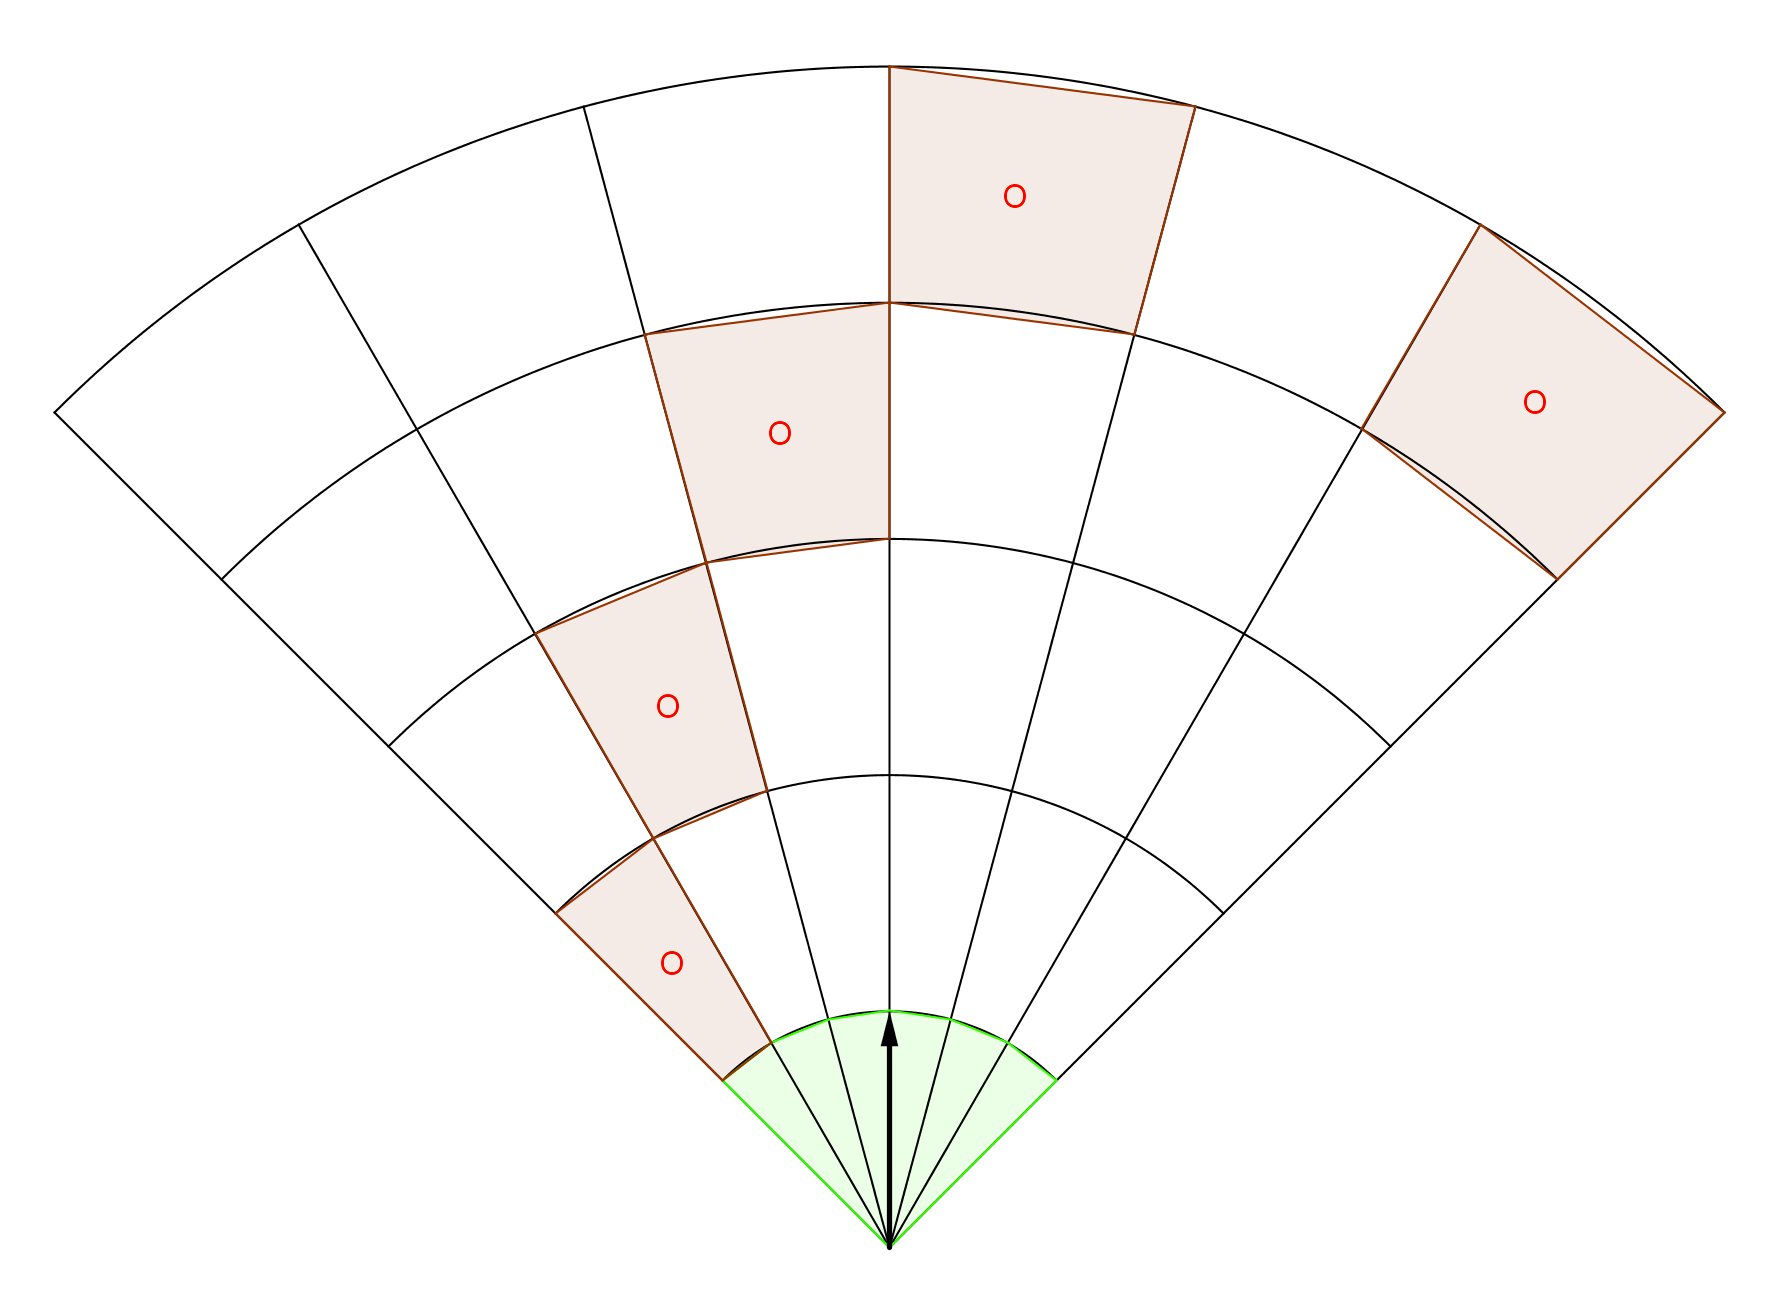
\includegraphics[width=0.9\linewidth]{\FIGDIR/CA001ObstacleDetection}
        \caption{Obstacle detection.}
        \label{fig:obstacleDetectionAvoidanceGrid}
    \end{subfigure}
    \begin{subfigure}{0.48\textwidth}
        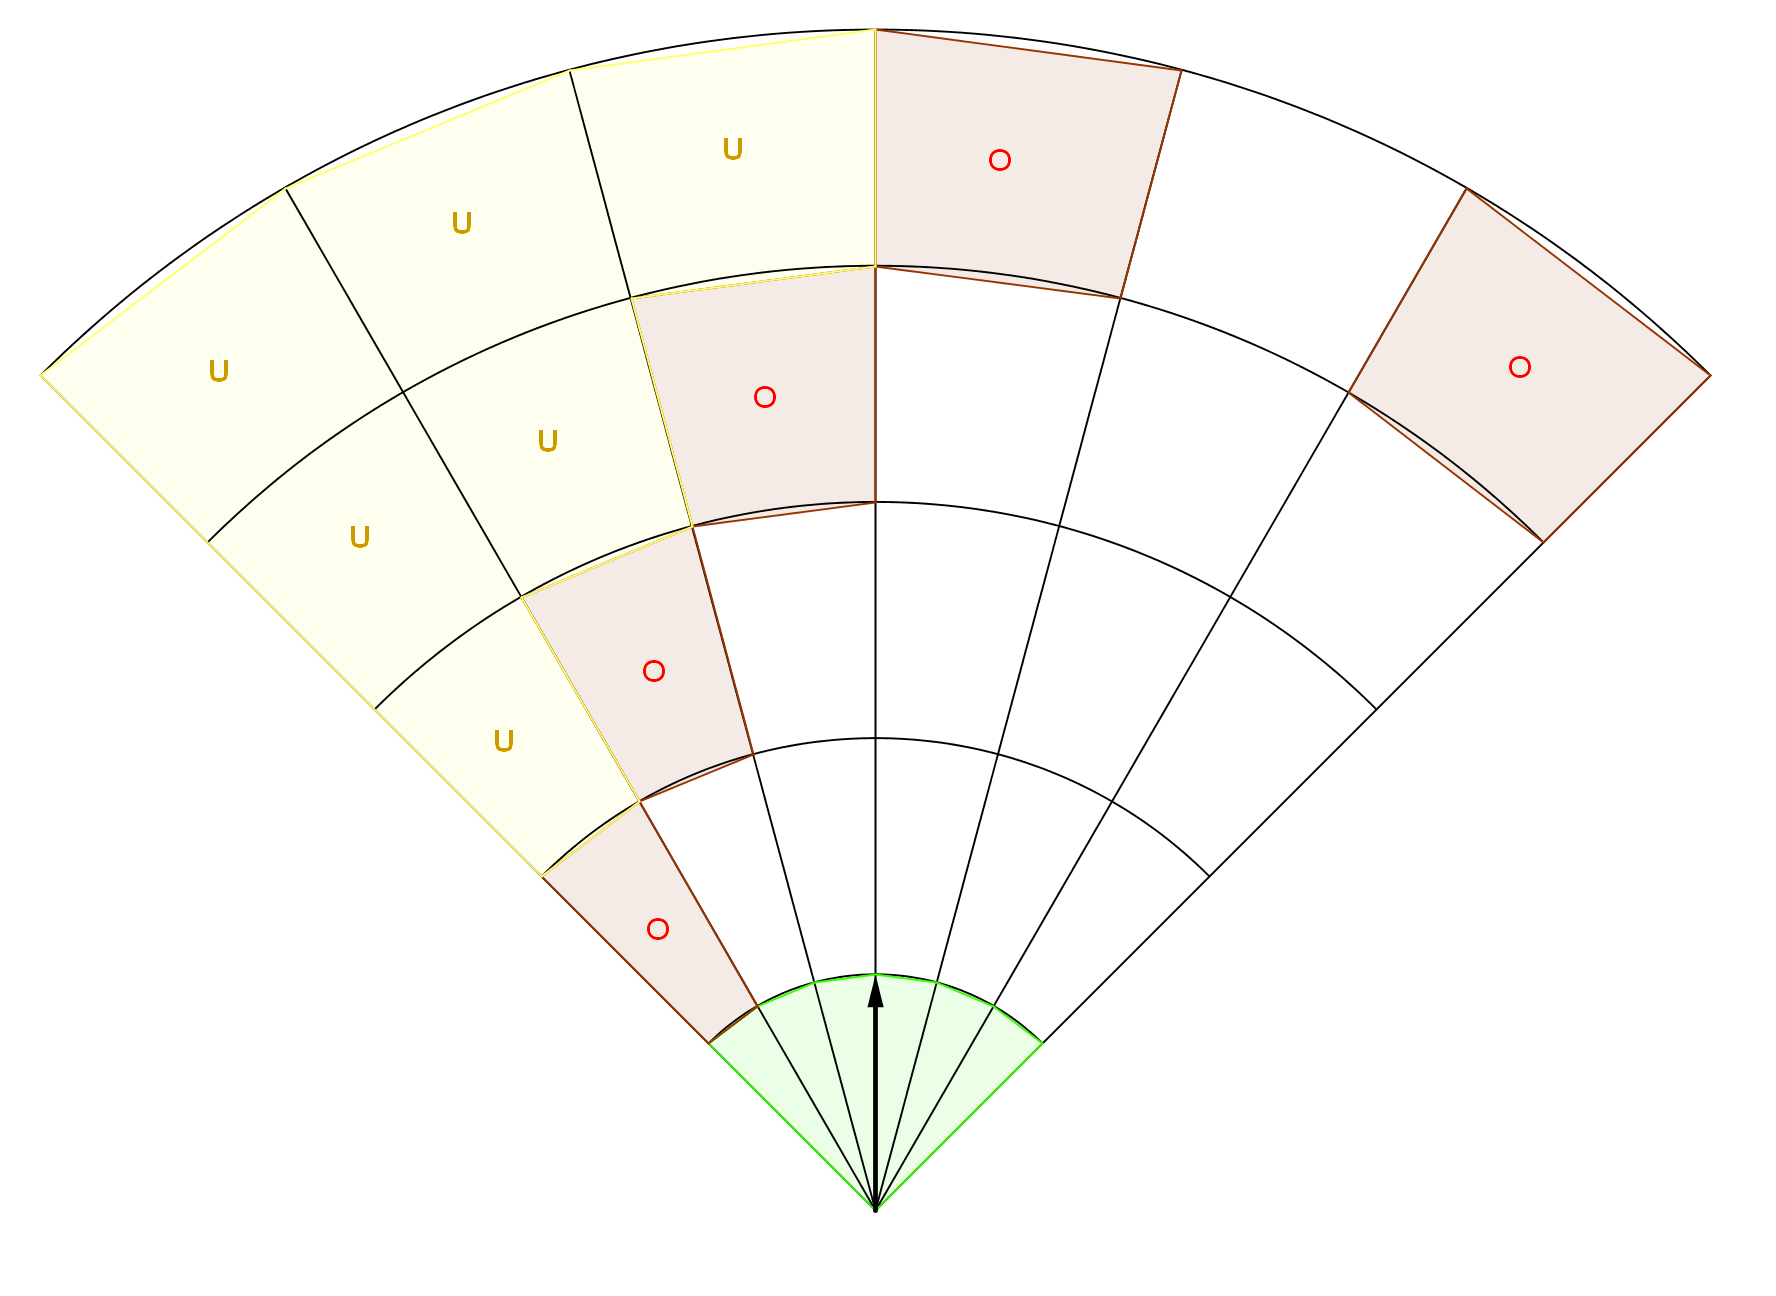
\includegraphics[width=0.9\linewidth]{\FIGDIR/CA002UncertainityAssesment} 
        \caption{Uncertainty assessment.}
        \label{fig:uncertainityAssesmentAvoidanceGrid}
    \end{subfigure}
    \\
    \begin{subfigure}{0.48\textwidth}
        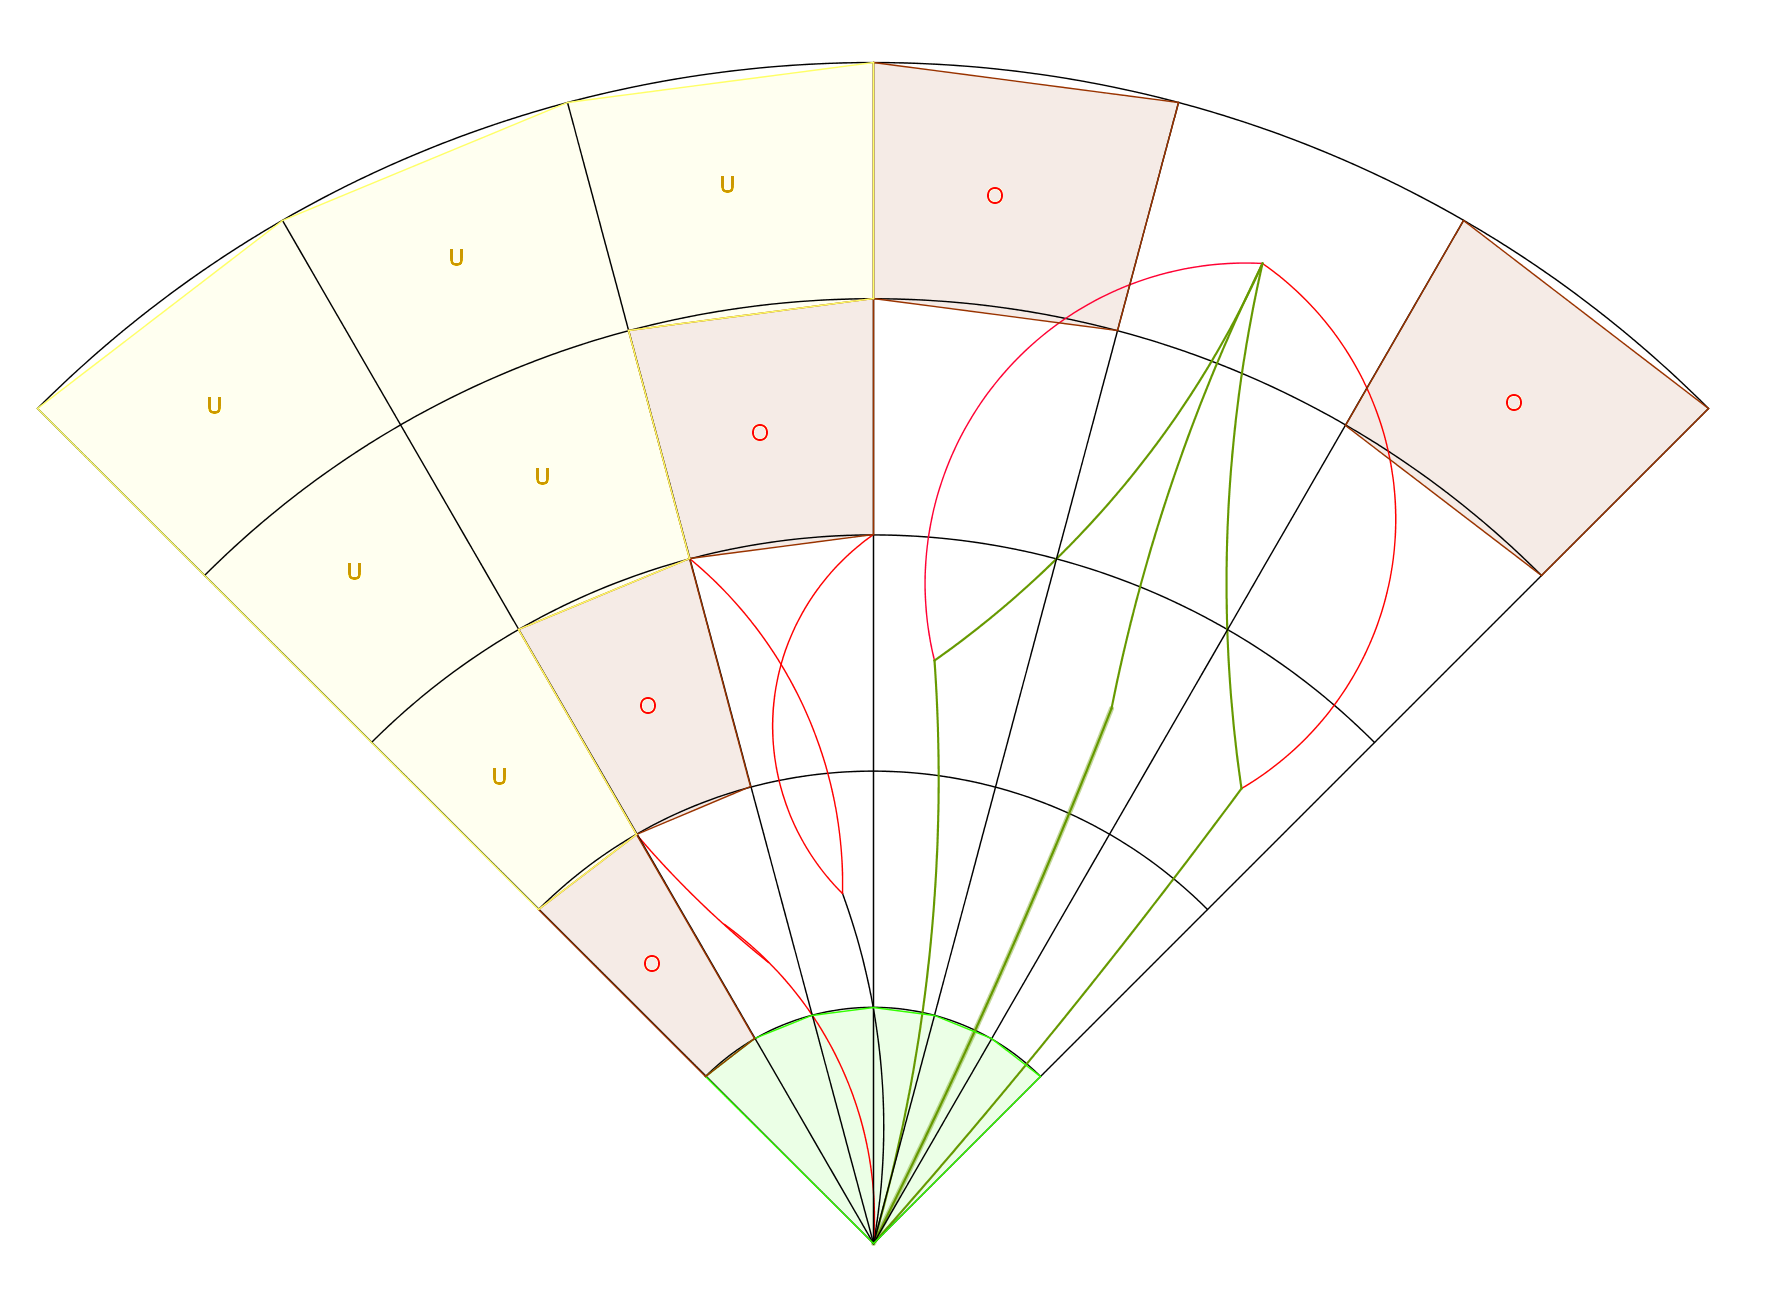
\includegraphics[width=0.9\linewidth]{\FIGDIR/CA003SurveyOfVacantSpace} 
        \caption{Trajectories reachibility evaluation.}
        \label{fig:trajectoriesSafetyEvaluationAvoidanceGrid}
    \end{subfigure}
    \begin{subfigure}{0.48\textwidth}
        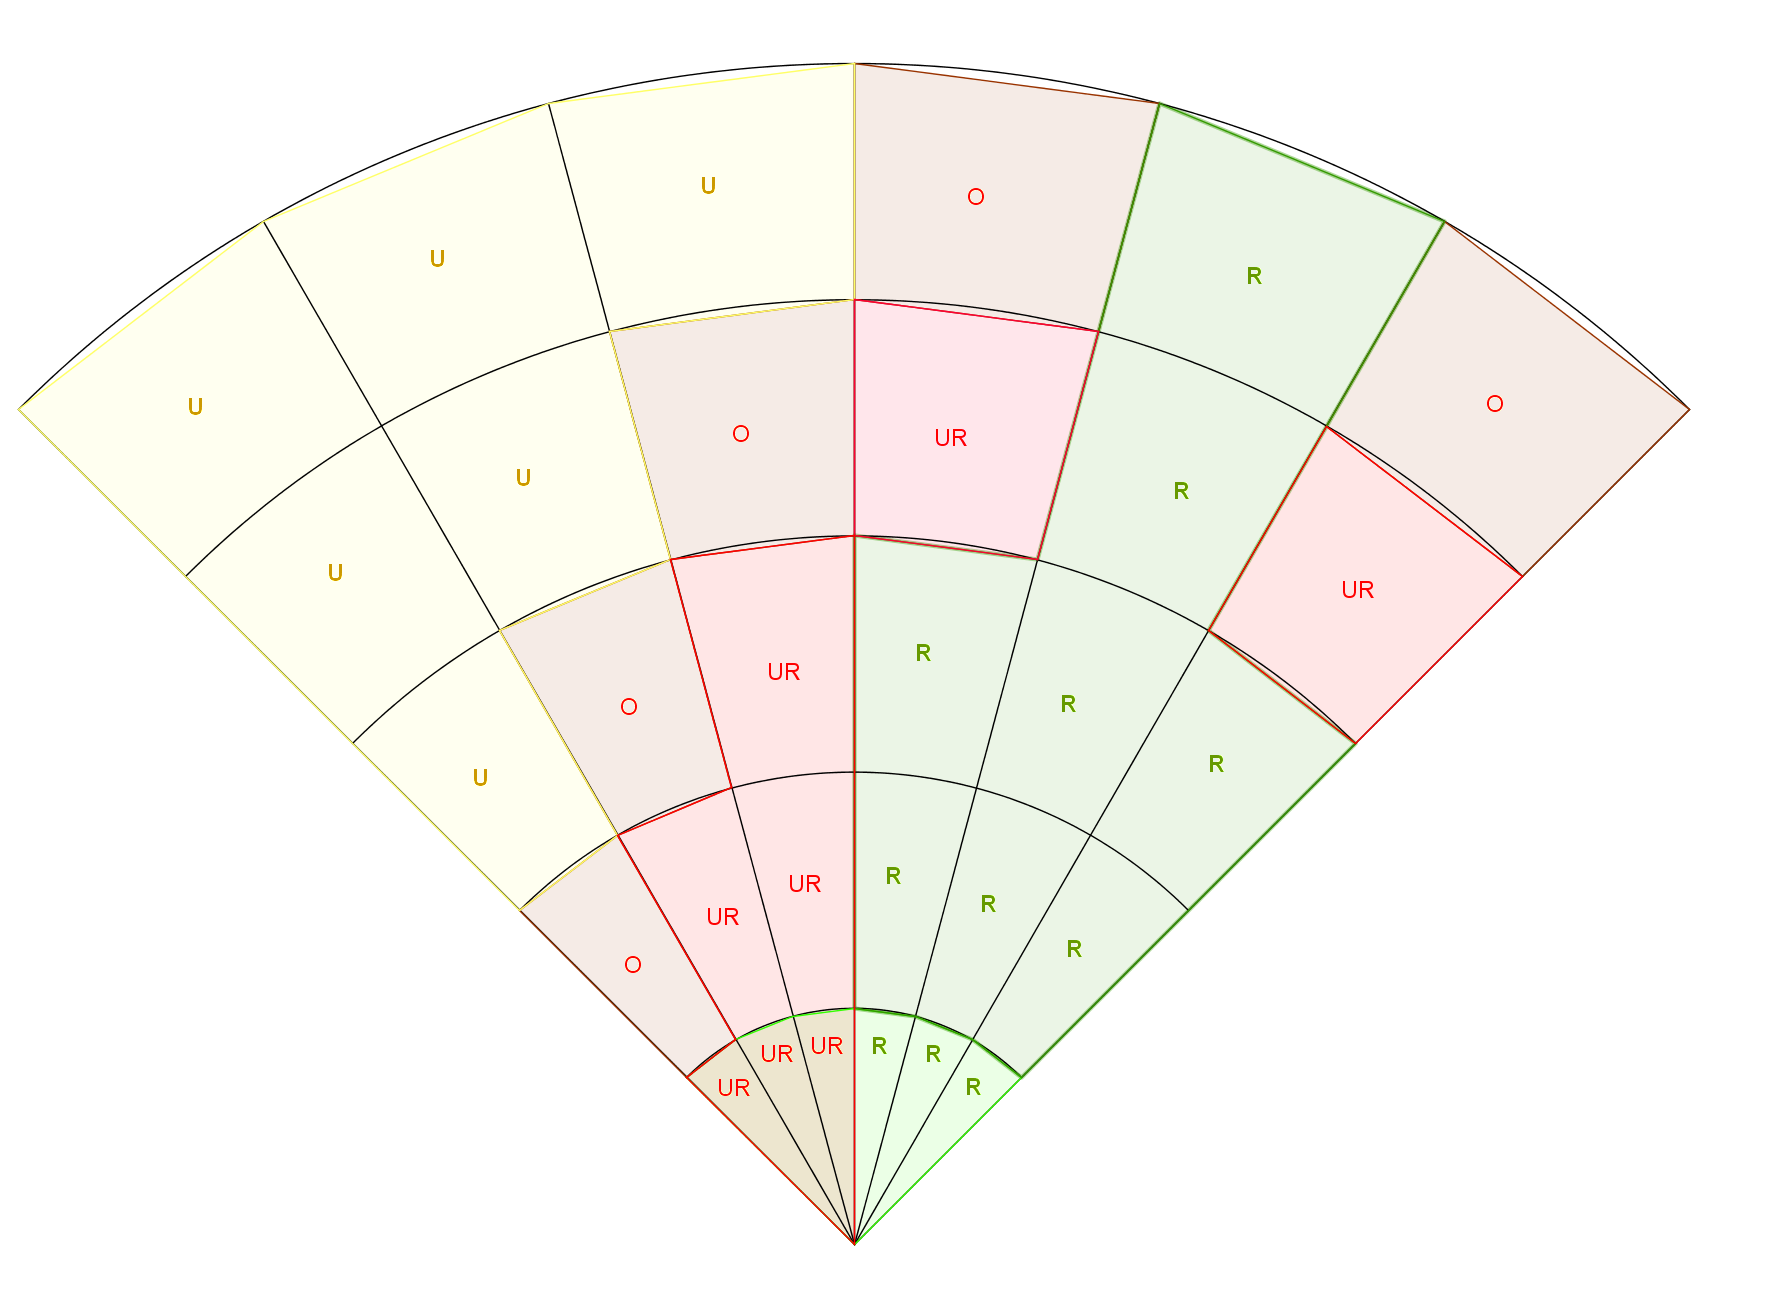
\includegraphics[width=0.9\linewidth]{\FIGDIR/CA004ReachableSpaceAssesment} 
        \caption{Cell reachibility evaluation.}
        \label{fig:reachibilityAssessmentAvoidanceGrid}
    \end{subfigure}
    \caption{Significant steps of \emph{Avoidance grid run} (inner loop).}
    \label{fig:significantStepsofAvoidanceGridRun}
\end{figure}

\begin{note}
    The \emph{Sensor Fusion Procedure} is solving all following steps (sec. \ref{s:sensorFusion}). The \emph{main purpose} of \emph{Avoidance Run} is finding best path under certain conditions.
\end{note}

\paragraph{Space Assessment Principle:} The \emph{Avoidance Grid} is fed trough \emph{Data Fusion} (sec. \ref{s:sensorFusion}). The process of \emph{ratings assessment} (tab. \ref{tab:defuzificationRatings}) is given in (fig. \ref{fig:significantStepsofAvoidanceGridRun}):
\begin{enumerate}
    \item \emph{Obstacle detection} (fig. \ref{fig:obstacleDetectionAvoidanceGrid}) - assessment of \emph{detected obstacles} (eq. \ref{eq:detectedObstacleRatingForCell}). The red (O) $cells$ have Detected obstacle set as \emph{true}. The other threats: \emph{map obstacles} (eq. \ref{eq:mapObstacleRatingForCell}), \emph{intruders} (eq. \ref{eq:intruderRatingForCell}), \emph{constraints} (eq. \ref{eq:constraintRatingForCell}) are false. The red (0) $cells$ are representing $Occupied(t_i)$ (eq. \ref{eq:ocuupiedDataFusion}) space in \emph{Avoidance Grid} at decision time $t_i$.
    
    \item \emph{Uncertainty assessment} (fig. \ref{fig:uncertainityAssesmentAvoidanceGrid}) - the uncertain cells are cells which status can not be \emph{assessed}. The \emph{Visibility} (eq. \ref{eq:visibilityForCell}) is low. The \emph{Uncertain} cells (yellow (U) mark) are equal to $Uncertain(t_i)$ (eq. \ref{eq:UncertainDataFusion}) in \emph{Avoidance Grid} in \emph{decision time} $t_i$. The $Constrained(t_i)$ (eq. \ref{eq:ocuupiedDataFusion}) space is equal to $\varnothing$ in this example.
    
    \item \emph{Trajectory reachibility evaluation} (fig. \ref{fig:trajectoriesSafetyEvaluationAvoidanceGrid}) - the \emph{Reach Set} given as \emph{Trajectory Set} (eq. \ref{eq:trajectoryTree}). is then projected trough \emph{Avoidance Grid} and pruned according to (def. \ref{def:PrunedReachSet}). \emph{Reachable Trajectories} (eq. \ref{eq:trajectoryReachibility}) are only those contained in $Free(t_i)$ space (eq. \ref{eq:freeDataFusion}). The \emph{Reachable Trajectories} are denoted as \emph{green lines}. The \emph{Unreachable} trajectory segments are denoted as \emph{red lines}. 
    
    \item \emph{Cell reachibility evaluation} (fig. \ref{fig:reachibilityAssessmentAvoidanceGrid}) - the evaluation of $cells$ reachibility is going according to (eq. \ref{eq:cellReachibility}). The \emph{Reachable cells} are those which \emph{contains} at least one \emph{Reachable Trajectory Segment}.
\end{enumerate}



\paragraph{Finding Best Path:} \footnote{Avoidance Run Function Implementation:\url{RuleEngine/MissionControl/MissionControl.m::findBestPath(avoidanceGrid)}} Each $cell_{i,j,k}$ in \emph{Avoidance Grid} at \emph{decision time} $t_i$ has assessed ratings according to \emph{data fusion procedure} (tab. \ref{tab:defuzificationRatings}). The following properties are know prior the \emph{trajectory} selection:
\begin{enumerate}
    \item \emph{Reachibility} for each  $cell_{i,j,k}$ (eq. \ref{eq:cellReachibility}).
    \item \emph{Reachibility} for each  $Trajectory(\circ)$ (eq. \ref{eq:trajectoryReachibility}).
    \item \emph{Free Space} as non empty set of $cells$ in \emph{Avoidance Grid} (eq. \ref{eq:freeDataFusion}), with \emph{Reachable Space} (eq. \ref{eq:ReachableDataFusion}).
    \item \emph{Goal Waypoint} $\mathscr{WP}_G$ from \emph{Mission Control Run} (sec. \ref{s:missionControlRun}).
\end{enumerate}

The \emph{Algorithm} (alg. \ref{alg:FindBestPathAvoidanceGrid}) is based on \emph{shortest path} search. Navigation is trying to reach \emph{goal waypoint}, therefore it tries to shorter distance between \emph{trajectory final cell} and \emph{goal waypoint}. If there is \emph{reachable space} two situations can occur:
\begin{enumerate}
    \item \emph{Goal waypoint is inside the Avoidance Grid} - the \emph{avoidance cell} is cell$_{i,j,k}$ containing \emph{goal waypoint} if reachable. 
    
    \item \emph{Goal waypoint is outside the Avoidance Grid} - the \emph{avoidance cell} is closest cell considered as \emph{outer cell} to \emph{goal waypoint}.
\end{enumerate}

\begin{note}
    \emph{Outer cell} is a cell$_{i,j,k}$ which has at least one \emph{wall} directly neighbouring with \emph{outer space} ($Universe - Known World (t_i)$). The \emph{outer cell} is selected to prevent navigation to the \emph{trap}.
\end{note}

The \emph{Avoidance Path} selection is simple lowest cost selection of \emph{Trajectory} $\in$ cell$_{i,j,k}$.
\newpage

\begin{algorithm}[H]
\SetKwInOut{Input}{Input}
\SetKwInOut{Output}{Output}
\Input{Cell[]  reachable (eq. \ref{eq:ReachableDataFusion}), Waypoint goal, AvoidanceGrid($t_i$) grid}
    
\Output{Trajectory avoidancePath, Error message}
    
    \BlankLine
    \# Initialization \& Reachibility test\;    
    avoidancePath = $\varnothing$\;
    \If{reachable ==  $\varnothing$}{        
        message = "No path available, empty Reach Set"\;
        \Return{[avoidancePath,message]}
    }
    avoidanceCell = GetRandomCell(reachable)\;
    
    \BlankLine
    \# Look for for goal cell\;
    \eIf{goal $\in$ grid}{
        \BlankLine
        \# Goal is inside Avoidance Grid, Check if reachable\;
        avoidanceCell = grid.selectCellXYZ(goal)\;
        \If{avoidanceCell.Reachable != true}{
            message = "Waypoint not Reachable"\;
            \Return{[avoidancePath,message]}
        }
    }{
        \BlankLine
        \# Goal is outside Avoidance Grid, look for closest reachable cell$_{i,j,k}$\;
        minimalDistance = distance(avoidanceCell,goal)\;
        \For{cell$_{i,j,k}$ $\in$ reachable}{
            
            \If{distance(cell$_{i,j,k}$,goal) $<$ minimalDistance}{
                \If{isOuterCell(cell$_{i,j,k}$)}{
                    minimalDistance = distance(cell$_{i,j,k}$,goal)\;
                    avoidanceCell = cell$_{i,j,k}$\;
                }
            }
        }
    }
    
    \BlankLine
    \# Reachable cell was found, Look for cheapest reachable trajectory\;
    avoidancePath = GetRandomTrajectory(avoidanceCell)\;
    \For{trajectory $\in$ avoidance Cell \&\& trajectory.Reachable == true}{
        \If{trajectory.Cost $<$ avoidancePath.cost}{
            avoidancePath = trajectory\;
        }
    }
   
    message = $\varnothing$\;
    \Return{[avoidancePath,message]}
    
    \caption{Find best \emph{Path} in \emph{Avoidance Grid}}
    \label{alg:FindBestPathAvoidanceGrid}    
\end{algorithm}

\newpage
\paragraph{Space Assessment Example:} For better understanding there is following example of \emph{space assessment} and \emph{Best Path Selection}. 


The \emph{UAS} (blue plane) is following \emph{mission plan} in open space. Then there is a detection of an \emph{collision situation} (fig. \ref{fig:exampleSituationAvoidanceRun}). The \emph{Obstacle} is detected in \emph{top-right} Avoidance Grid corner. 

The \emph{LiDAR hits} are denoted as red filled circles. The \emph{Avoidance Grid} space is constrained by black dashed line. The \emph{Avoidance Grid} is separated into 5 layers going from top to \emph{bottom}. The \emph{Reach Set} is projected as a set of \emph{Trajectories} with colorization. 

\begin{figure}[H]
\centering
    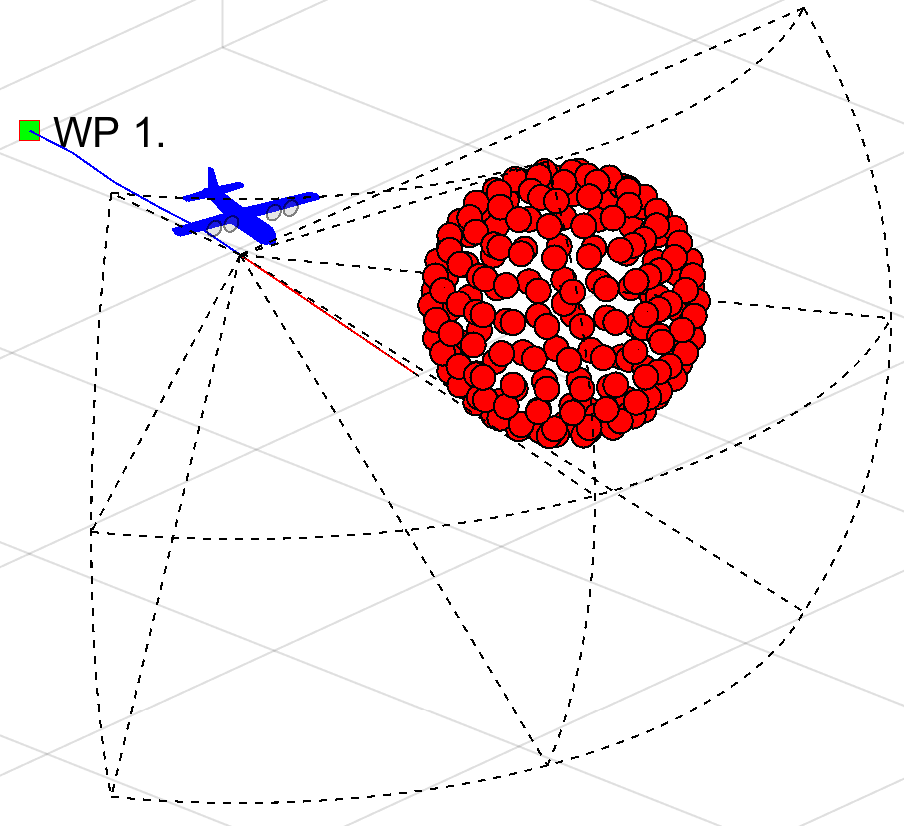
\includegraphics[width=0.75\linewidth]{\FIGDIR/TE038AvoidanceRunExample}        
    \caption{Example: The situation to be evaluated by \emph{Avoidance Run}.}
    \label{fig:exampleSituationAvoidanceRun}
\end{figure}
\newpage
\noindent\emph{Visibility Assessment:} The visibility assessment (fig. \ref{fig:exampleVisibilityEvaluation}) divides the \emph{Avoidance Grid} into two
\begin{enumerate}
    \item \emph{Visible space} (blue filled cells) is space \emph{trough} which \emph{LiDAR} rays roamed freely until they hit an \emph{Obstacle}.
    
    \item \emph{Uncertain space} (black filled cells) is space where no \emph{LiDAR ray} passed nor hit. Therefore its status is uncertain.
\end{enumerate}
 
 \begin{note}
     The \emph{detected obstacle cells} are part of \emph{visible space}, because there is certainty about its containment.
 \end{note}
 
 The \emph{Reach Set} trajectories are colored based on their visibility, blue for \emph{uncertain} trajectories and \emph{green} for visible trajectories.

\begin{figure}[H]
    \centering
    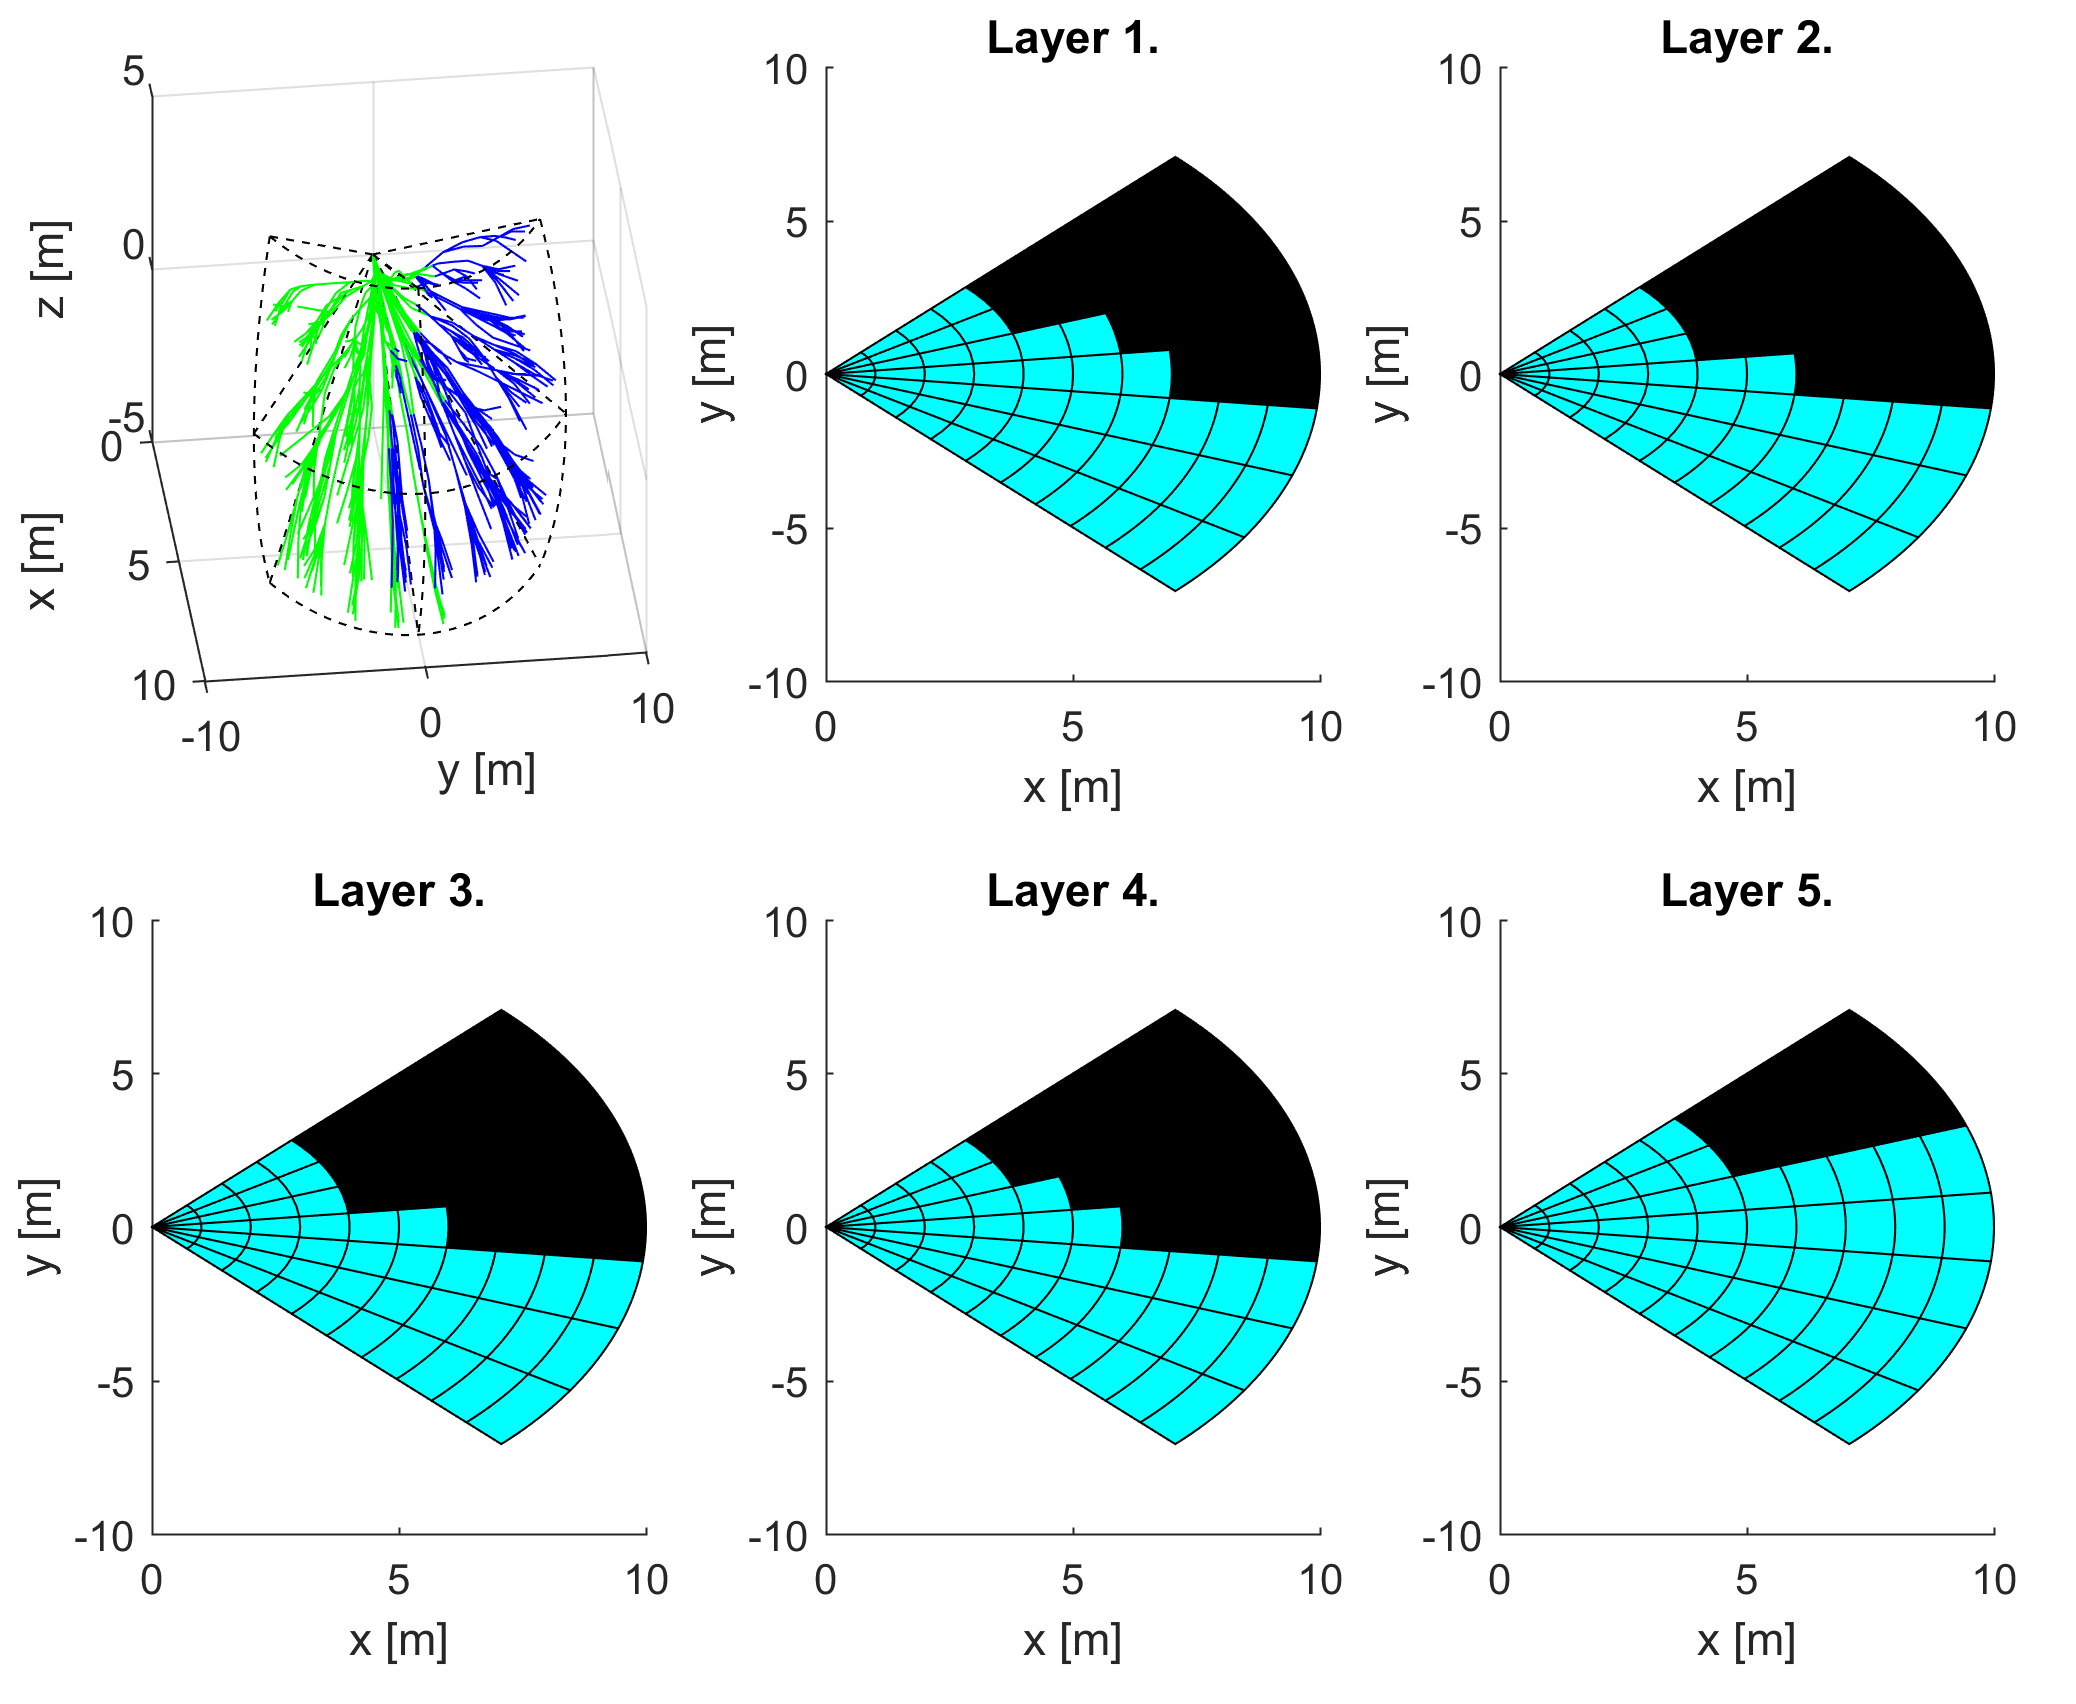
\includegraphics[width=0.95\linewidth]{\FIGDIR/TE040Visibility}        
    \caption{Example: The \emph{Visibility} evaluation by \emph{Avoidance Run}.}
    \label{fig:exampleVisibilityEvaluation}
\end{figure}

\newpage
\noindent\emph{Reachibility Assessment:} For Each trajectory the \emph{Reachibility} is assessed (fig. \ref{fig:exampleReachibilityEvaluation}). The \emph{Obstacle Space} and \emph{Uncertain Space} are rendering \emph{reachibility}, effectively separating \emph{trajectories} into two categories:

\begin{enumerate}
    \item \emph{Unreachable Trajectories} (red lines) - there is at least one trajectory segment leading trough \emph{Obstacle} or \emph{Uncertain} space.
    
    \item \emph{Reachable Trajectories} (green lines) -  all trajectory segments are lying in \emph{Free} space.
\end{enumerate}

Cells in Avoidance grid are divided in similar matter, depending on count of \emph{reachable trajectories} passing trough them:

\begin{enumerate}
    \item \emph{Unreachable Cells} (red fill) - there is no trajectory trough \emph{free space} or the \emph{cell} is not in \emph{free space}.
    
    \item \emph{Reachable cells} (green fill) - there is at least one \emph{feasible trajectory} reaching \emph{free cell}.
\end{enumerate}

\begin{figure}[H]
    \centering
    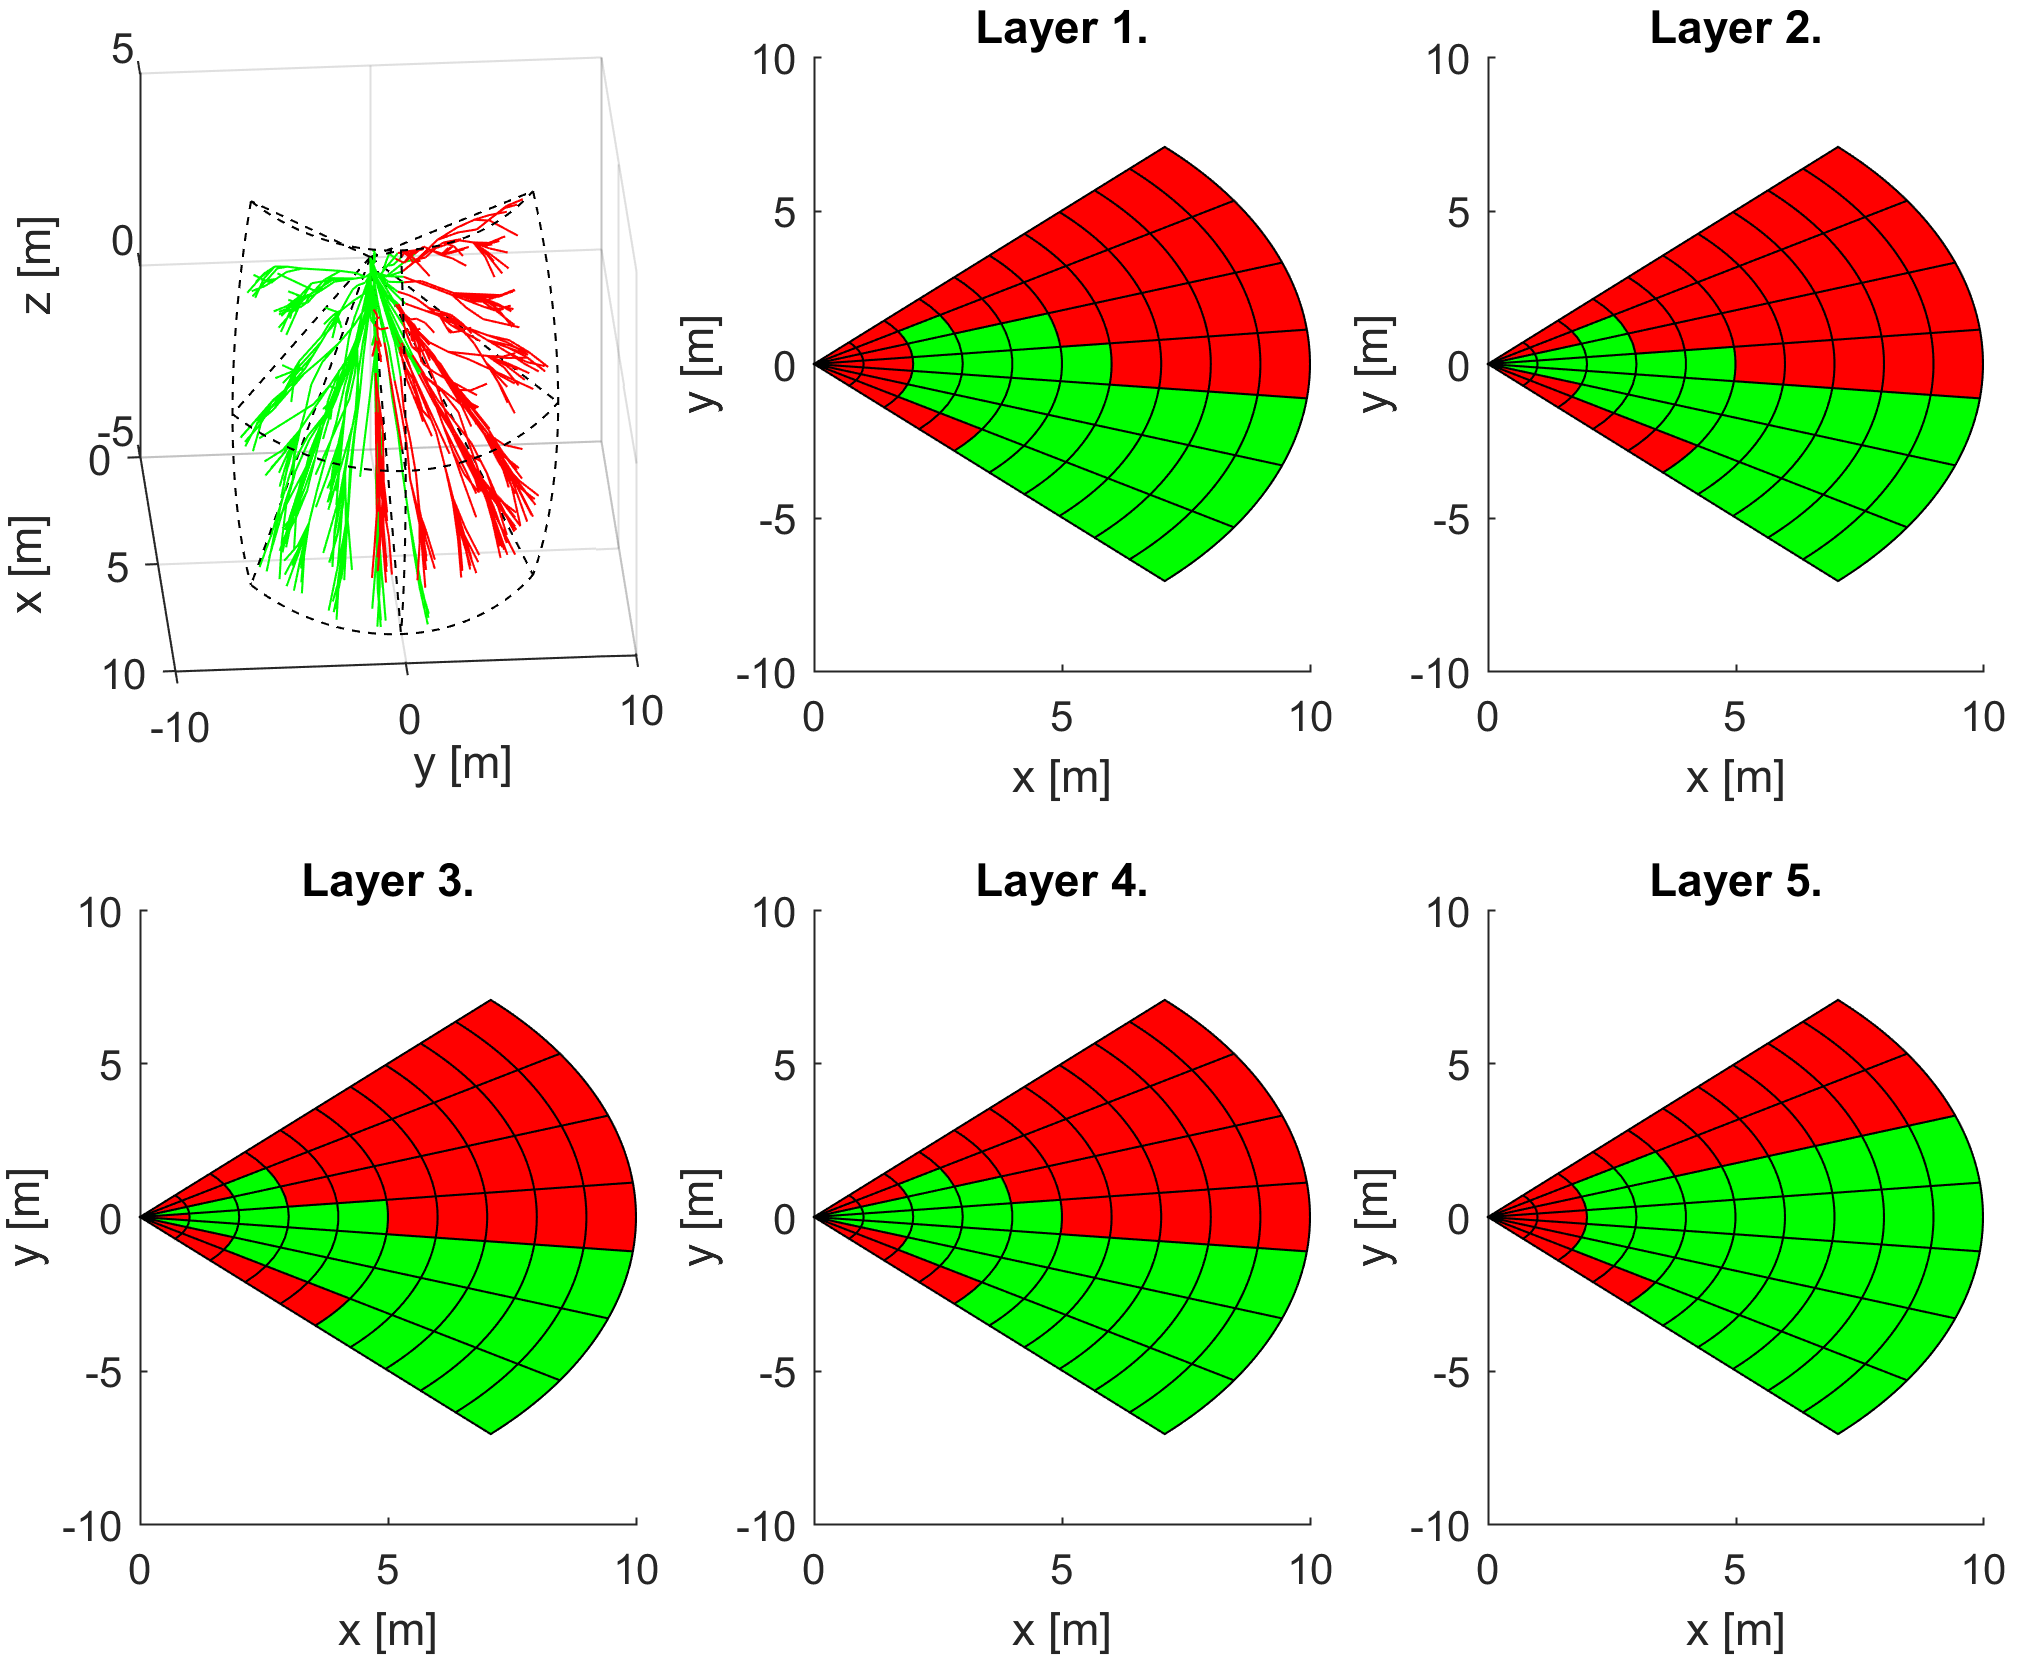
\includegraphics[width=0.95\linewidth]{\FIGDIR/TE041Reachibility}        
    \caption{Example: The \emph{Reachibility} evaluation by \emph{Avoidance Run}.}
    \label{fig:exampleReachibilityEvaluation}
\end{figure}

\begin{note}
    The \emph{best avoidance path} is selected form \emph{reachable outer cells} (green fill in fig. \ref{fig:exampleReachibilityEvaluation}), depending on \emph{goal waypoint} according to (alg. \ref{alg:FindBestPathAvoidanceGrid}).
\end{note}
    	\newpage
\subsection{\secState{R}Mission Control Run}\label{s:missionControlRun}
\paragraph{Introduction and Motivation:}  This section will introduce \emph{Navigation Concept} using  \emph{Reach Set Approximation}. The \emph{Avoidance Framework Concept} (fig. \ref{fig:AvoidanceFrameworkConceptNew}) defines \emph{Navigation Module} as \emph{sub-system} for long term \emph{trajectory tracking}.  The \emph{Avoidance Grid Run} (sec. \ref{s:aviudabceGridRun}) is solving the \emph{Path Search} problem inside operation space constrained by \emph{Avoidance Grid} for time $t_i$. 

There is a need to build a trajectory between \emph{Waypoints} which are further away than \emph{distance} of one \emph{Avoidance Grid}.  The \emph{UAS} is controlled via \emph{Movement Automaton}. The \emph{Movements} which are in \emph{Movement Buffer} can be replaced with another movements. This feature of \emph{Movement Automaton} is called \emph{Movement Chaining} (eq. \ref{eq:movementChaining}).

To join the multiple \emph{Avoidance Grids} paths following terminology needs to be established (fig. \ref{fig:missionControlRunExample}):
\begin{enumerate}
    \item \emph{Goal} (Selecting Goal of Navigation) - the point where UAS want to get in global coordinate frame. The selection needs to be defined.
    
    \item \emph{Next Decision} - the point when the next \emph{Avoidance Grid Run} is applied. The outline of events and triggers is required. The \emph{decision} will be made in \emph{next decision time} $t_{i+1}$.
\end{enumerate}

\noindent The \emph{Avoidance Grid} from \emph{UAS} viewpoint can be separated into following zones (fig. \ref{fig:gridZonesMissionControl}):
\begin{enumerate}
    \item \emph{Crash Area} (last layers) - there is no place for safe return and the \emph{border} of \emph{Avoidance Grid} is near. The \emph{Decision Point} needs to lie before this zone.
    
    \item \emph{Avoidance Area} (middle layers) - the area of \emph{Active Avoidance Maneuvering}. The \emph{Reach Set Approximation} performance (sec. \ref{s:ReachSetPerformanceCriteria}) is important in this area.
    
    \item \emph{Safe Zone} (first layers) - there is space for safe return or damage mitigation.
\end{enumerate}

\begin{figure}[H]
    \centering
    \begin{subfigure}{0.48\textwidth}
        \centering
        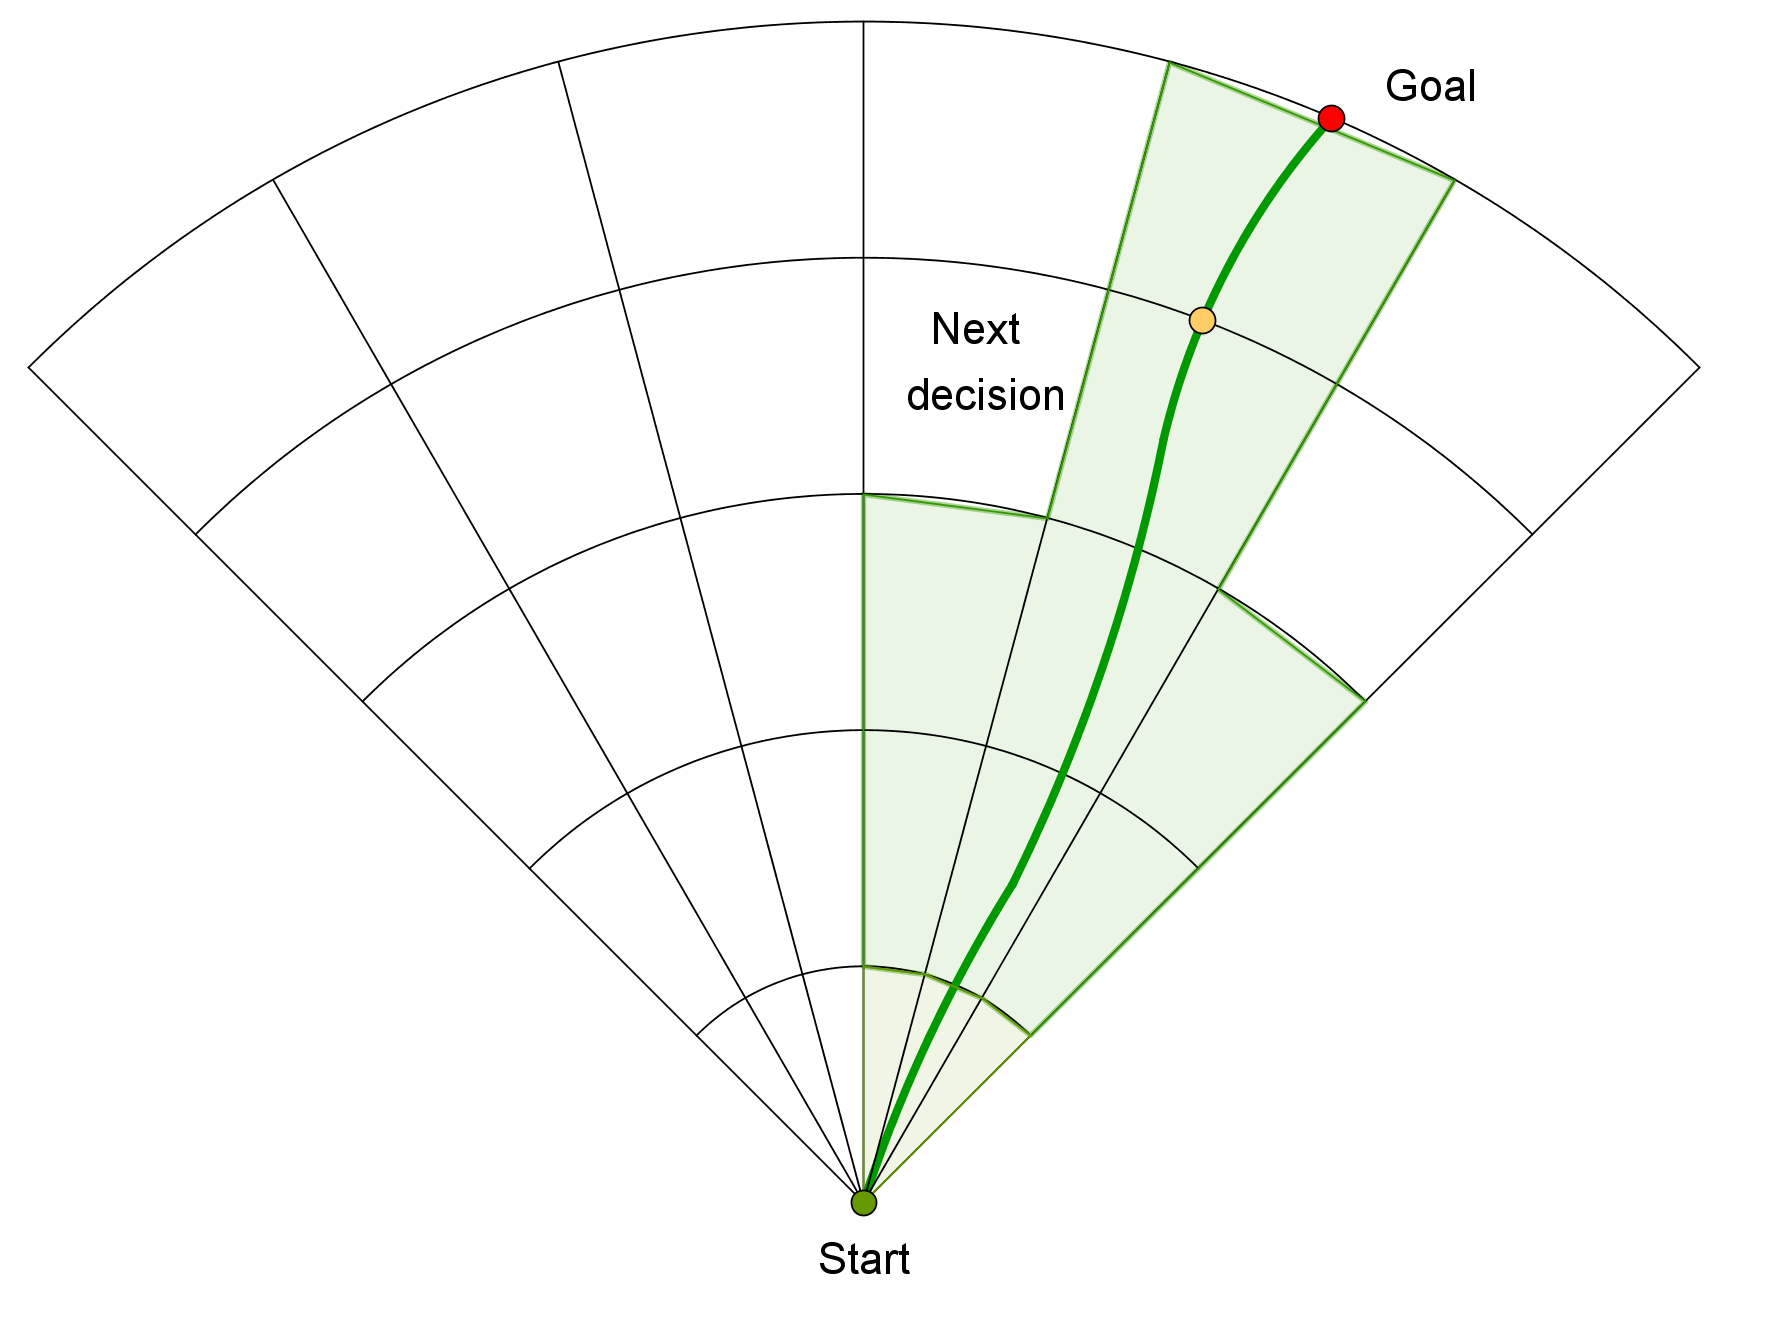
\includegraphics[width=0.9\linewidth]{\FIGDIR/CA005PathCalculation}
        \caption{Mission control run example.}
        \label{fig:missionControlRunExample}
    \end{subfigure}
    \begin{subfigure}{0.48\textwidth}
    	\centering
        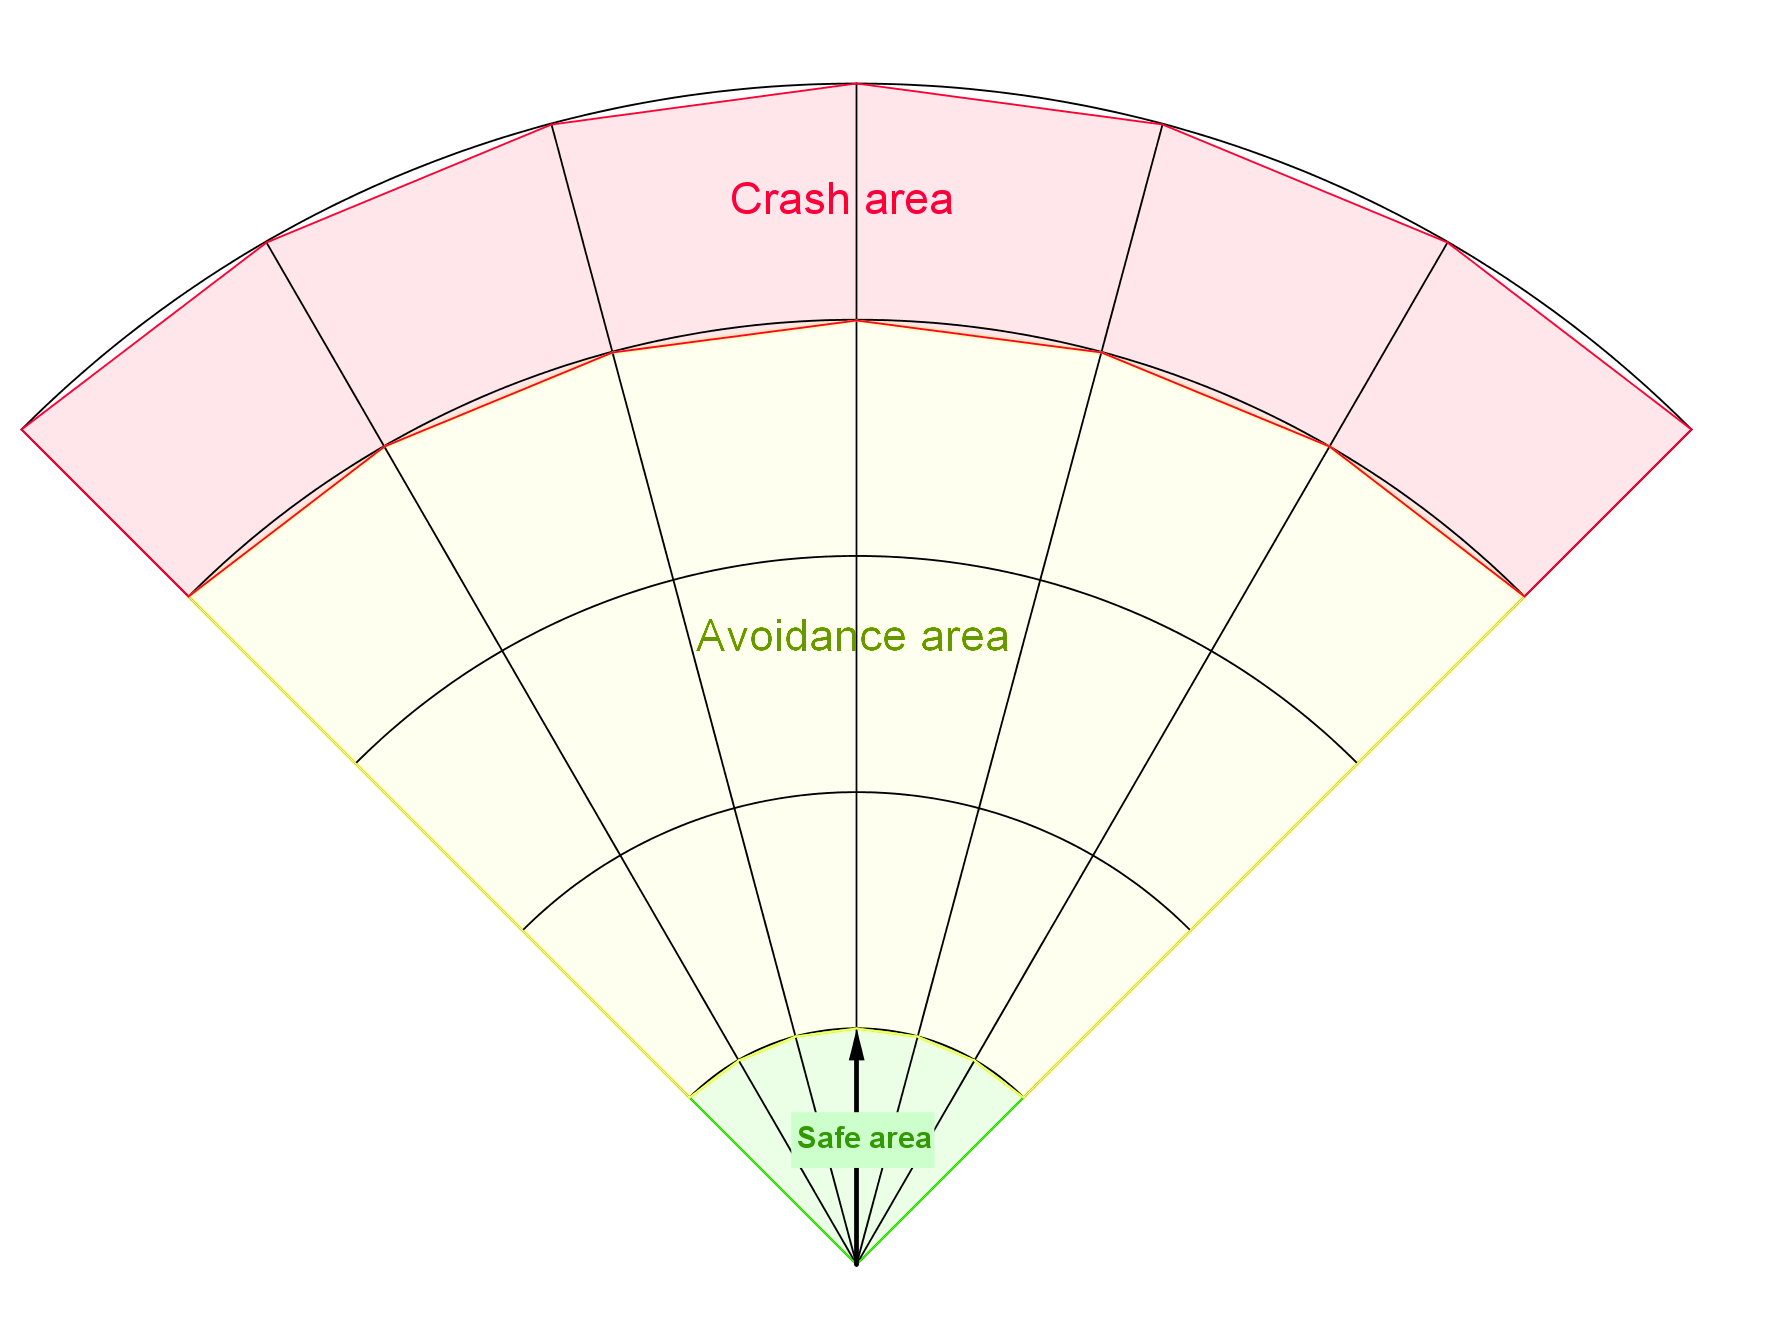
\includegraphics[width=0.9\linewidth]{\FIGDIR/CA006FieldOfViewZones} 
        \caption{Grid Zones.}
        \label{fig:gridZonesMissionControl}
    \end{subfigure}
    \caption{Definitions for \emph{Mission Control Run} (outer loop).}
    \label{fig:definitionsForMissionControlRun}
\end{figure}

\noindent Joining \emph{Avoidance Grid Runs} (fig. \ref{fig:joiningMultipleAGRS})  example portrays \emph{Avoidance Grid Runs} invoked on various \emph{Decision Points} to achieve \emph{Navigation} functionality. The UAS (blue plane) is flying Mission (green numbered waypoints). The \emph{Avoidance Grid} boundary (black dashed line) for each \emph{Decision Point} (UAS position at time $t_i$). Following example of \emph{Navigation} (fig. \ref{fig:missionControlRunActivityDiagram}) run is shown:

\begin{enumerate}
    \item \emph{Mission Start} (fig. \ref{fig:missionExampleWithOAGR}) - UAS at the start of the mission have one \emph{Avoidance Grid} at its position to determine the \emph{Navigation Path} to \emph{Waypoint 2} (goal waypoint). The planned path (red line) is leading directly to \emph{Avoidance Grid} boundary (black dashed line).
    
    \item \emph{Mission End} (fig. \ref{fig:finishedMissionAGR}) - UAS have reached 
    \emph{last waypoint}. All \emph{Avoidance Grid} boundaries (black dashed line) for all \emph{runs} are drawn along flown trajectory. 
    
    \item \emph{Waypoint Reach} (fig. \ref{fig:waypointReachAGR}) - the \emph{waypoint} is inside \emph{Avoidance Grid}, the navigation path (red line) leads directly to \emph{goal waypoint}. (Excessive \emph{Avoidance Grid} boundaries are removed.)
    
    \item \emph{Next Waypoint} (fig. \ref{fig:newtWaypointAGR}) - the new \emph{Goal Waypoint} is selected, the UAS moves to new goal (invoking \emph{Avoidance Grid Runs} when necessary).
    
\end{enumerate}

\begin{figure}[H]
    \centering
    \begin{subfigure}{0.48\textwidth}
        \centering
        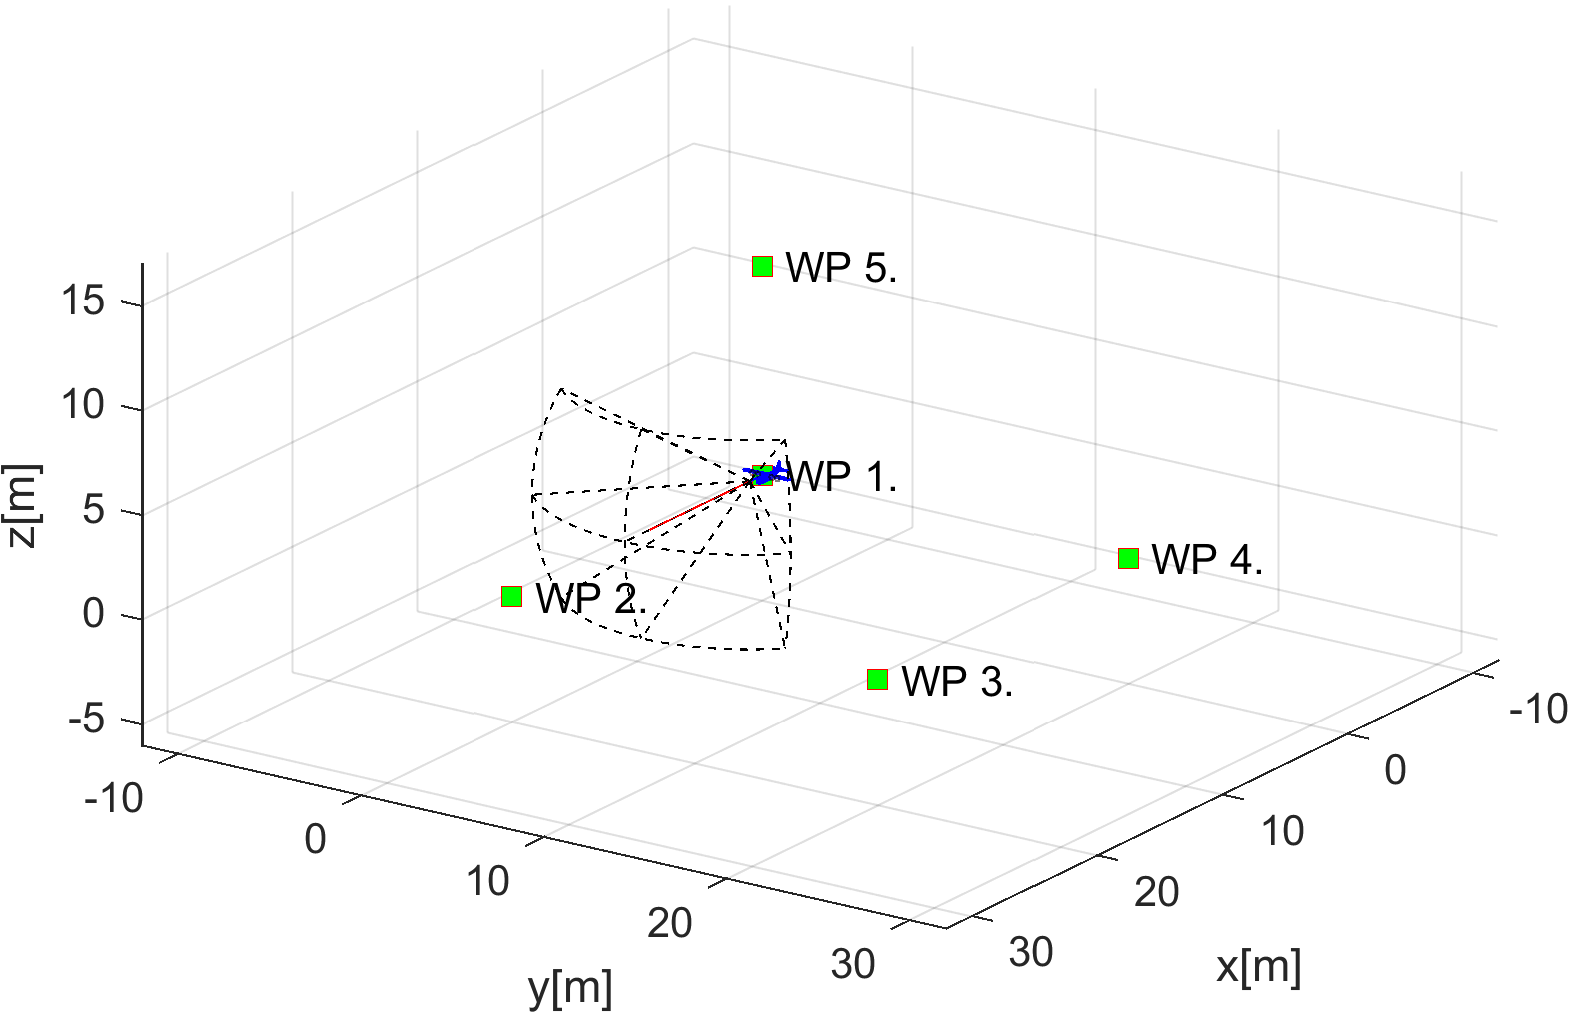
\includegraphics[width=0.9\linewidth]{\FIGDIR/TE042MissionExample}
        \caption{Mission start.}
        \label{fig:missionExampleWithOAGR}
    \end{subfigure}
    \begin{subfigure}{0.48\textwidth}
    	\centering
        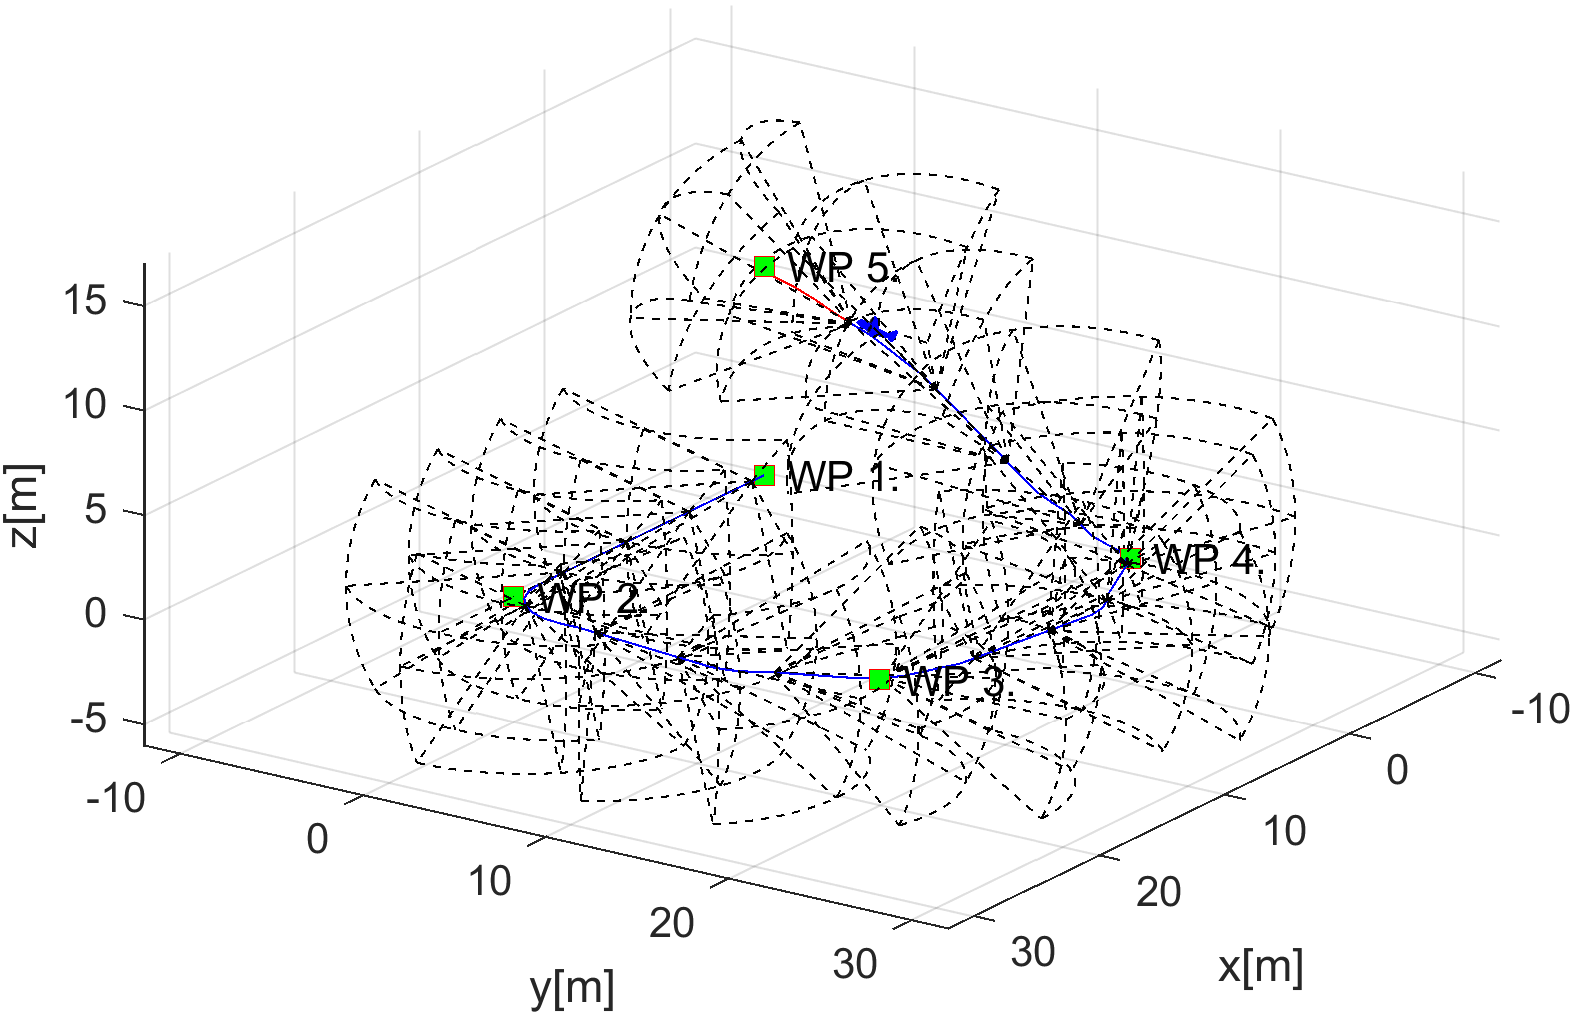
\includegraphics[width=0.9\linewidth]{\FIGDIR/TE043AllDecisionDecisionPoint} 
        \caption{Mission end.}
        \label{fig:finishedMissionAGR}
    \end{subfigure}
    \\
    \centering
    \begin{subfigure}{0.48\textwidth}
        \centering
        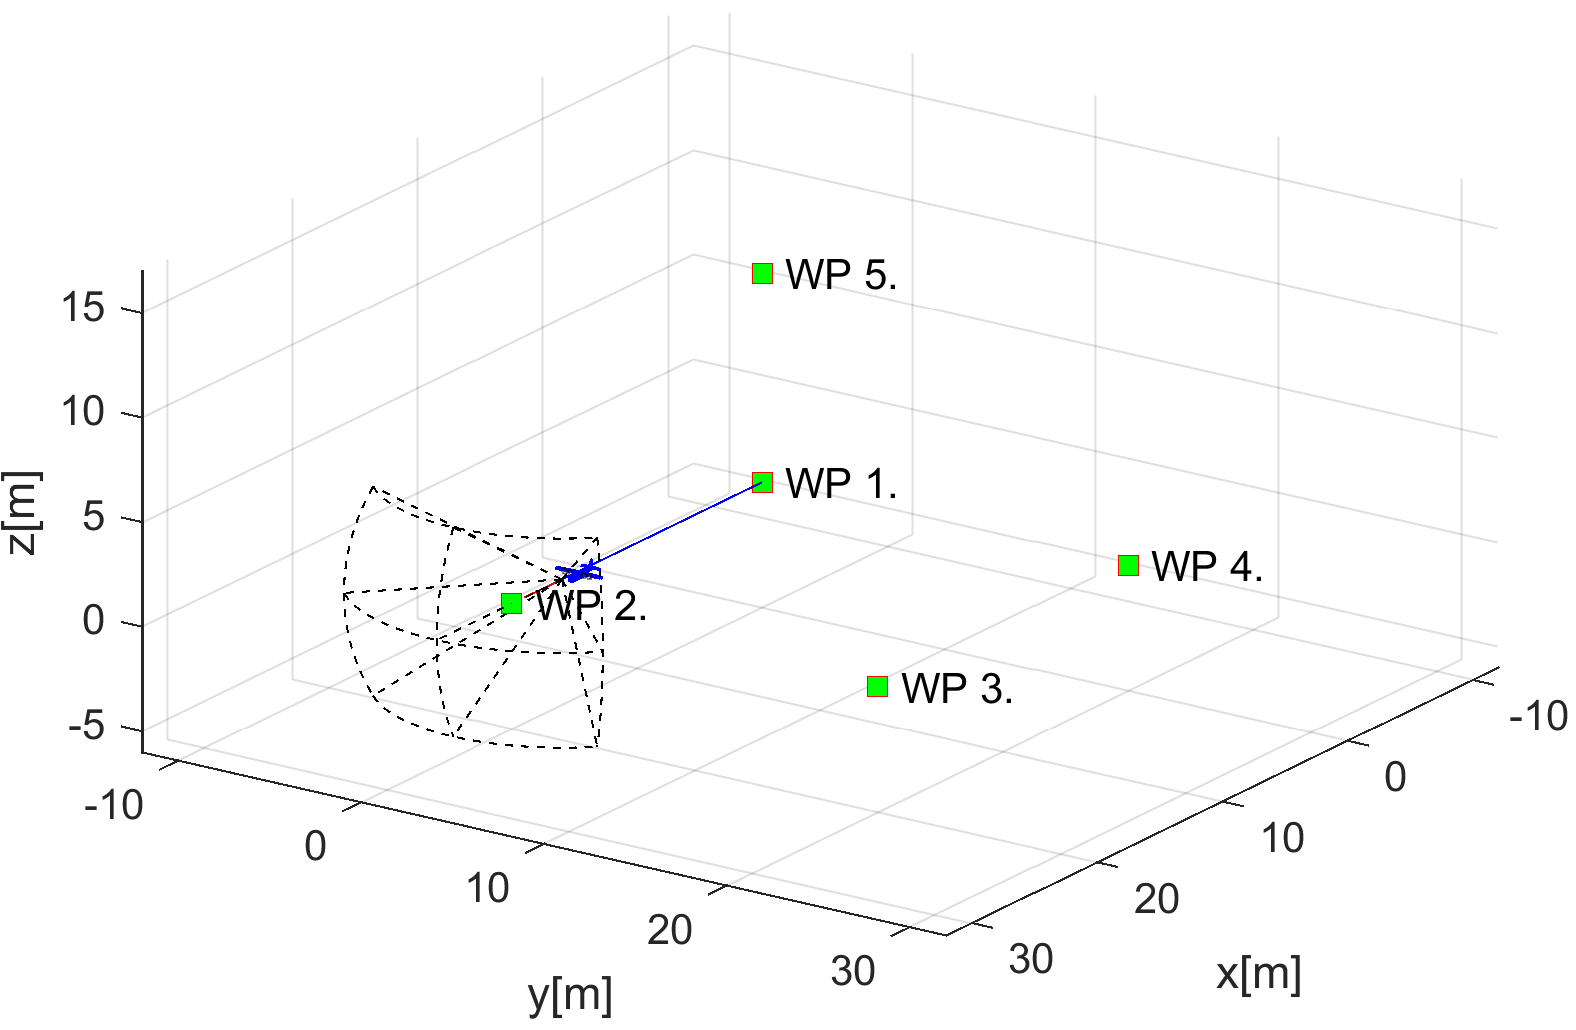
\includegraphics[width=0.9\linewidth]{\FIGDIR/TE044WaypointReach}
        \caption{Waypoint reach.}
        \label{fig:waypointReachAGR}
    \end{subfigure}
    \begin{subfigure}{0.48\textwidth}
    	\centering
        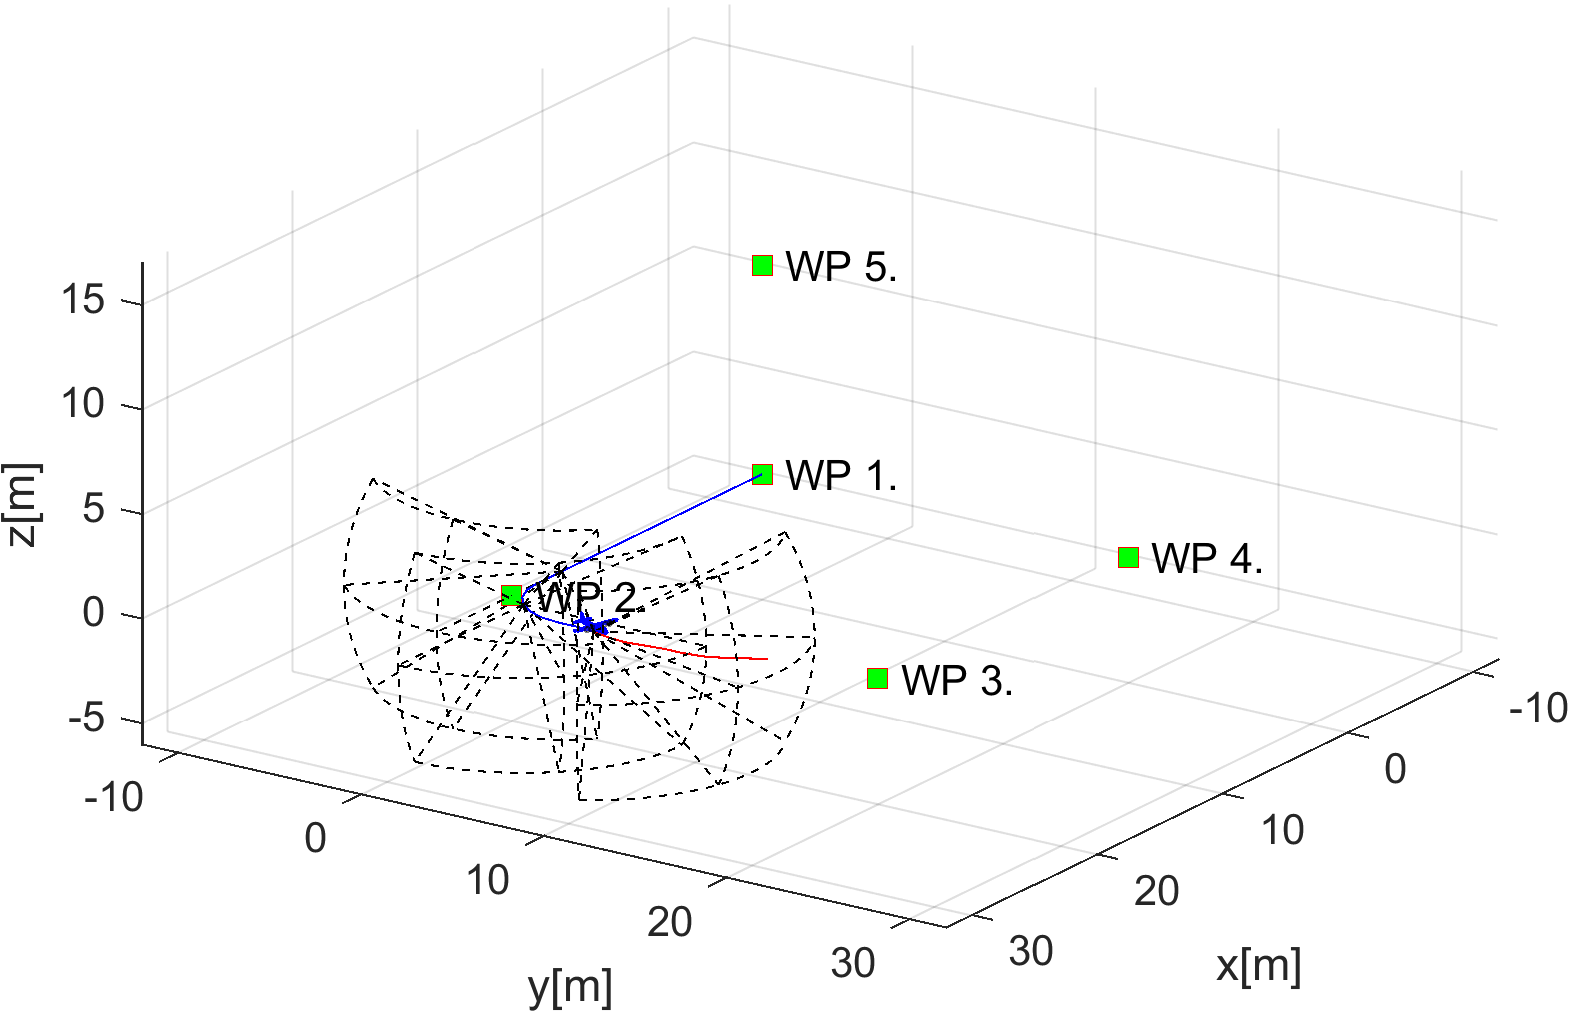
\includegraphics[width=0.9\linewidth]{\FIGDIR/TE045NewWaypointSetup} 
        \caption{Next waypoint.}
        \label{fig:newtWaypointAGR}
    \end{subfigure}
    \caption{Joining multiple \emph{Avoidance Grid Runs} for achieve Navigation.}
    \label{fig:joiningMultipleAGRS}
    
\end{figure}
    

\newpage
\paragraph{General Concept:}\footnote{Mission Control Run Function Implementation: \url{RuleEngine/MissionControl/MissionControl.m::runOnce(.)}} The \emph{General Concept} is taken from  \cite{sabatini2014navigation,Sabatini2014}, consisting from following main modules:
\begin{enumerate}
    \item \emph{Navigation Loop} - module responsible for \emph{Navigation} providing \emph{Goal Waypoint}.
    
    \item \emph{Data Fusion} (background in sec. \ref{s:sensorFusion}) - module responsible for \emph{Surveillance Data Feed}.
    
    \item \emph{Situation Assessment} - module responsible for \emph{UAS Safety Evaluation}. 
    
    \item \emph{Avoidance Run} (background in sec. \ref{s:aviudabceGridRun}) responsible for \emph{Avoidance Path} selection.    
\end{enumerate}


\begin{figure}[H]
    \centering
    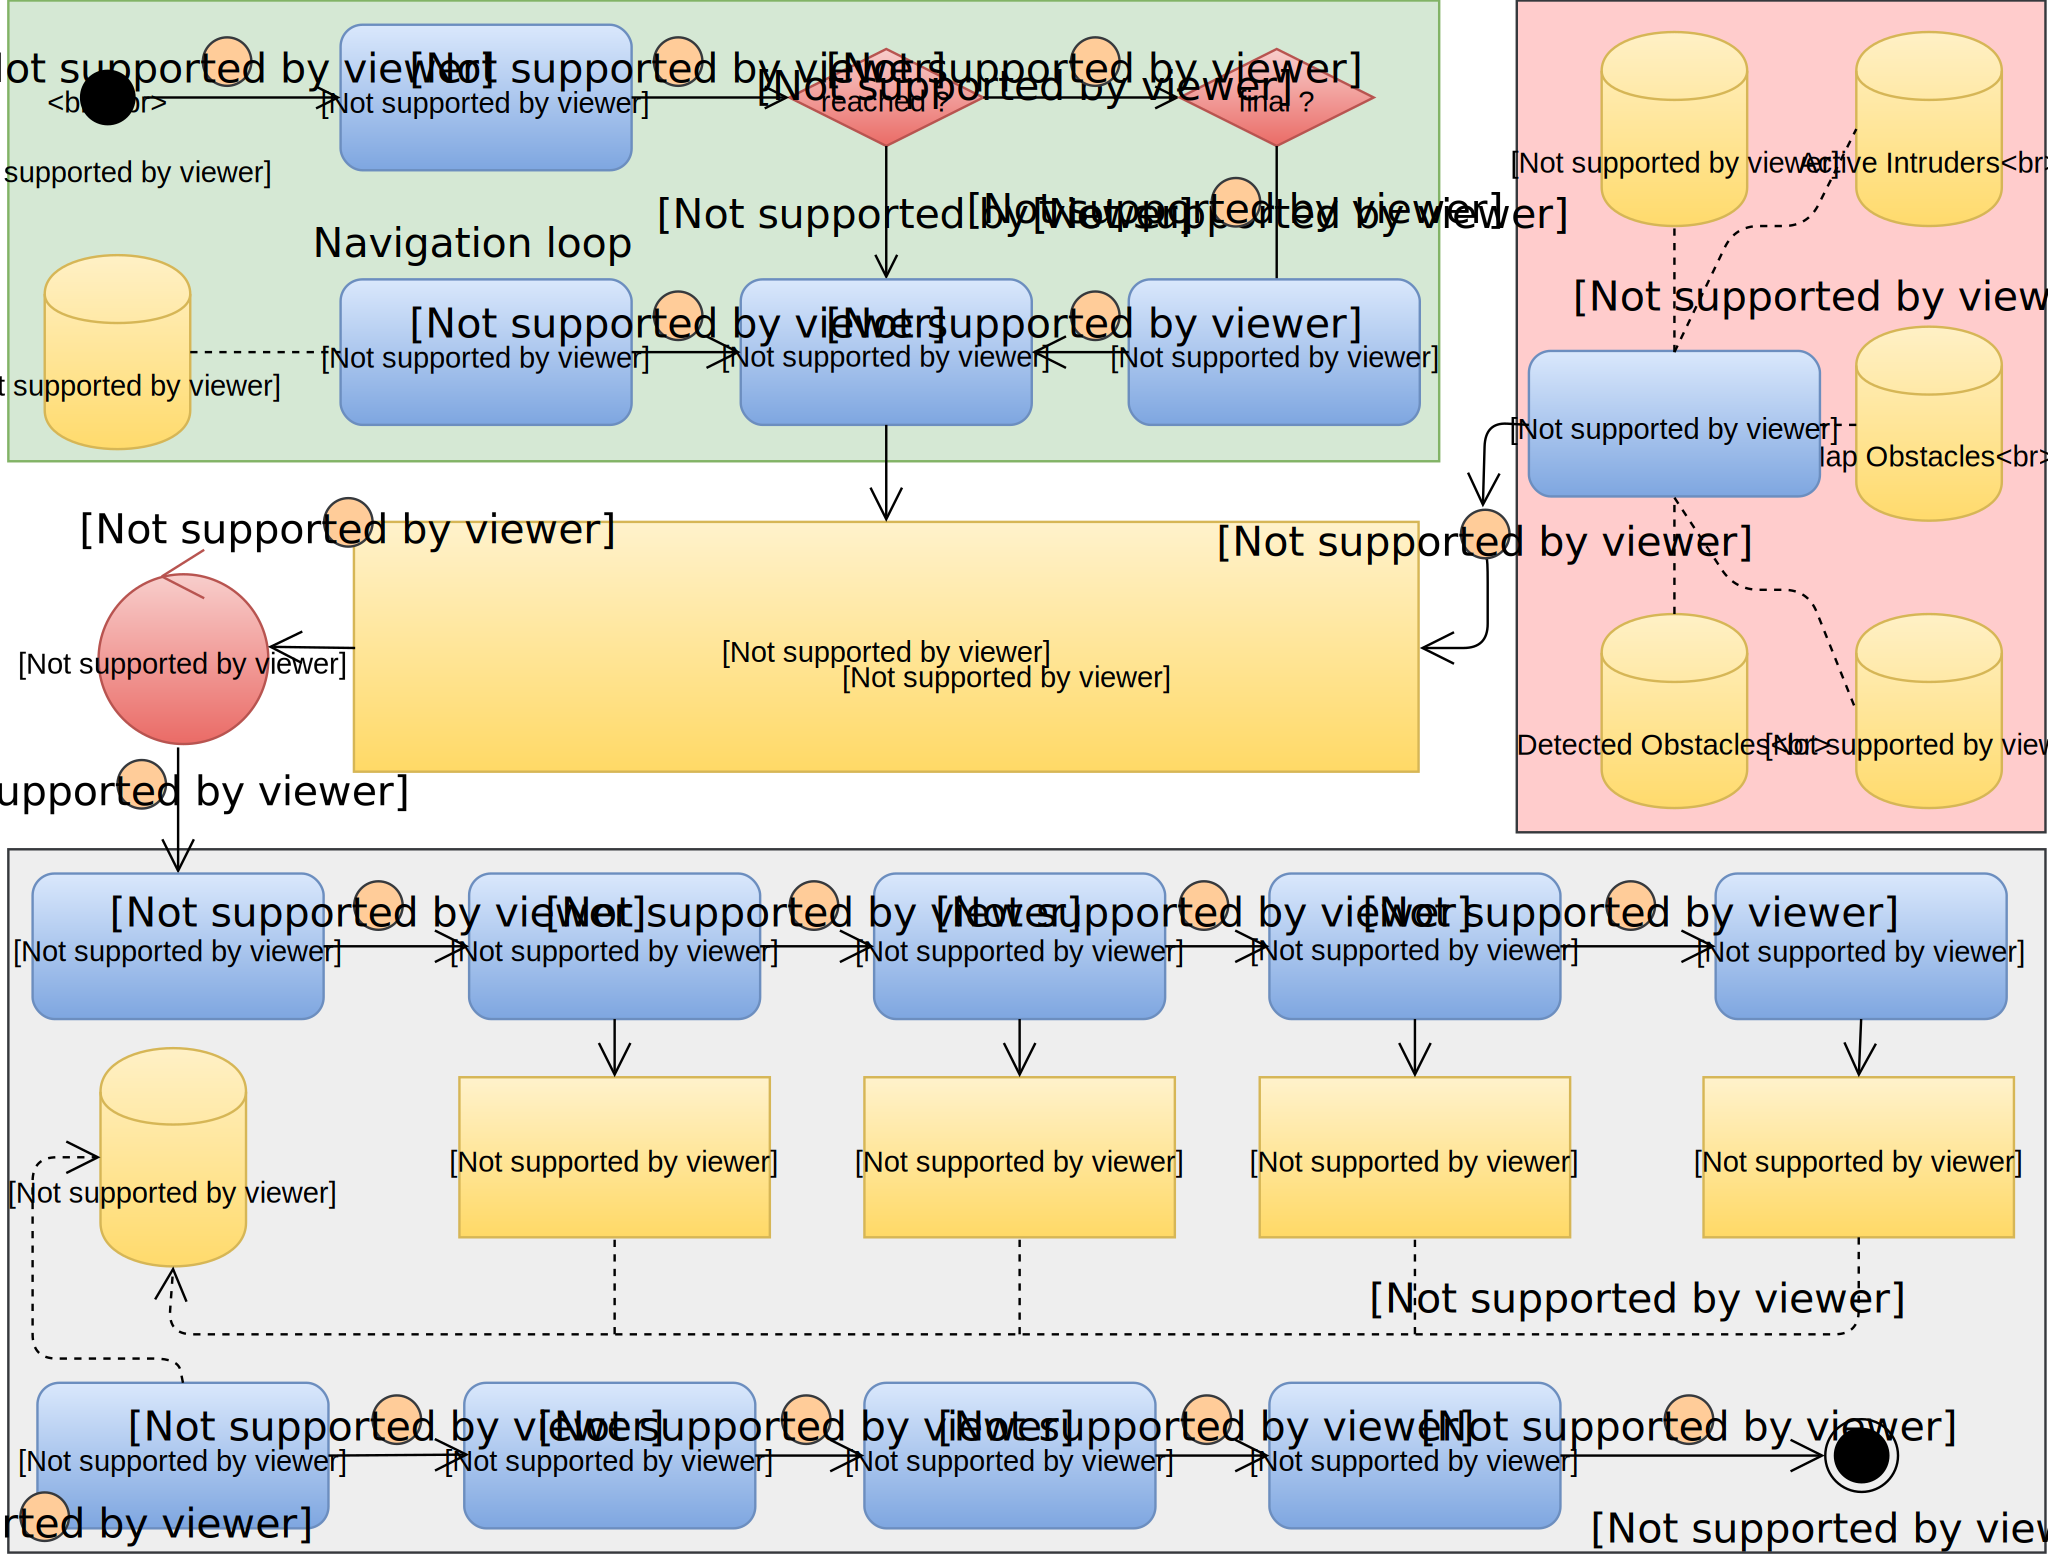
\includegraphics[width=\linewidth]{\FIGDIR/TE026AvoidanceAlgorithmMainLoopRun}
    \caption{Mission control run activity diagram.}
    \label{fig:missionControlRunActivityDiagram}
\end{figure}

\noindent The main changes to \emph{Navigation architecture} are given in \emph{Mission Control Run} activity diagram (fig. \ref{fig:missionControlRunActivityDiagram}):

\begin{enumerate}
    \item \emph{Situation Assessment} - added event-based mode switching control. 
   
    \item \emph{Avoidance Run} - added hierarchical evaluation for \emph{Avoidance Path} selection. Prioritizing threat avoidance according to a type. 
\end{enumerate}

\noindent The \emph{Operation Mode} is introduced, based on \emph{Situation assessment} and \emph{Triggering Events} one of following modes are selected in \emph{Avoidance Run}:

\begin{enumerate}
    \item \emph{Navigation Mode} - the \emph{UAS} is navigating through \emph{Airspace} following \emph{cost effective patterns} and obeying \emph{Airspace Authority} (UTM). The \emph{Navigation Grid} is a instance of \emph{Avoidance Grid} (sec. \ref{s:AvoidanceGrid}) with initialized \emph{Navigation Reach Set} (ex. \emph{Harmonic Reach Set Approximation} (sec. \ref{s:harmonicReachSet})).
    
    \item \emph{Emergency Avoidance Mode} - the \emph{UAS} is \emph{threatened} by obstacle, intruder, hard constraint or \emph{soft constraint}, the \emph{UAS} is navigating through \emph{Airspace} following \emph{safe avoidance patterns} and \emph{minimizing the impact} of possible damages. The \emph{Avoidance Grid} is term used for \emph{Emergency Avoidance Mode}. The \emph{Avoidance Reach Set Approximation} is initialized in \emph{Avoidance Grid} (ex. \emph{Chaotic Reach Set Approximation} (sec. \ref{s:chaoticReachSet}))
\end{enumerate}

\begin{note}
    Depending on \emph{Operation Mode} the pair of \emph{Avoidance Grid} and \emph{Reach Set} is selected in \emph{Avoidance Run} part.
    
    
    The \emph{Navigation Grid} and \emph{Avoidance Grid} shares the space segmentation pattern, therefore the \emph{Data Fusion} (sec. \ref{s:sensorFusion}) needs to be evaluated only once for both grids. 
\end{note}



\paragraph{Decision Time Frame ($[t_i,t_{i+1}[$):} The \emph{Mission Control Run} is executed for \emph{Decision Time Frame} bounded to the \emph{period} of the \emph{UAS executed movement} (fig. \ref{fig:AvoidanceFrameworkConceptNew}).

The \emph{UAS System} (sec. \ref{s:UASNonlinearModel}) controlled by \emph{Movement Automaton Implementation} (sec. \ref{s:movementAutomatonDefinition}) \emph{Planned Movements} can be changed at any time. The real impact on control is shown after the \emph{actual movement} is executed. 

\begin{note}
    For our \emph{Movement Automaton Implementation} movements the average \emph{movement duration} is \emph{1/velocity second} (tab. \ref{tab:movements1}, \ref{tab:movements2}).
\end{note}

The \emph{Decisions} are made based on \emph{system} state in \emph{current} time-frame started at $t_i$ for \emph{next} time frame starting at $t_{i+1}$.

\begin{note}
    Because the \emph{Decision Delay} is crucial in \emph{Avoidance System} it is beneficial to have \emph{short time movements}. On the other hands, the \emph{length and duration  of movements} is impacting \emph{Reach Set Complexity}. The proper construction of movement automaton is greatly impacting overall \emph{approach performance}.
\end{note}

\paragraph{Initialization:} The \emph{UAS} is going to solve a problem for \emph{Rules of the Air} (eq. \ref{eq:rulesOfTheAir}). Using control scheme (fig. \ref{fig:AvoidanceFrameworkConceptNew}) with given \emph{Sensors}:

\begin{equation}
    Sensors = \{LiDAR,ADS-B\}
\end{equation}

\noindent The sensors obstacle assessment into avoidance grid is outlined for static obstacles in (sec. \ref{s:staticObstacles}) and for moving obstacles in (sec. \ref{s:intruders}.)

\noindent The \emph{Data Fusion Procedure} is given as follow:
\begin{equation}
    DataFusion = \{Rating Based Data Fusion \quad (sec. \ref{s:sensorFusion})\}
\end{equation}

Then the \emph{UAS system} (sec. \ref{s:UASNonlinearModel}) with \emph{Movement Automaton Implementation} (sec. \ref{s:movementAutomatonDefinition}) with empty movement buffer:

\begin{equation}
    Movement Buffer = \{\}
\end{equation}

\noindent The \emph{Avoidance Grids} for both \emph{Operation Modes} are created with \emph{identical space segmentation}. The \emph{Reach Set Approximations} are loaded based on initial \emph{UAS State} at decision time $0$. The \emph{Reach Set Approximation} is always selected based on \emph{UAS System State}. The initial \emph{Operation Mode} is set up as \emph{Navigation}. The initialization is summarized like follow:

\begin{equation}
    \begin{aligned}
    Avoidance Grid(0) &= \{UAS.position(0),AvoidanceReachSet(UAS.ReachSet)\}\\
    Navigation Grid (0) &= \{UAS.position(0), NavigationReachSet(UAS.ReachSet)\}\\
    Operation Mode &= Navigation
    \end{aligned}
\end{equation}

The \emph{Mission} is set up as a set of \emph{ordered waypoints}. The \emph{initial goal waypoint} is \emph{first waypoint}. The initialization is summarized like follow:

\begin{equation}
    \begin{aligned}
    Mission &= \{Waypoint_1 \dots  Waypoint_n\}\\
    Goal Waypoint &= Mission.waypoint_1\\
    Last Waypoint &= Mission.waypoint_n\\
    \end{aligned}
\end{equation}

The \emph{actual threats} are set as empty sets for \emph{decision time} $t_i=0$:
\begin{equation}
    \begin{aligned}
    obstacles &= \{\}, intruders = \{\}, hard Constraints = \{\}, soft Constraints = \{\}\\
    \end{aligned}
\end{equation}



\paragraph{Navigation Loop (1\textsuperscript{st}-3\textsuperscript{rd} step):} The purpose of \emph{Navigation Loop} is to select proper \emph{Goal Waypoint} from \emph{Mission} (sec. \ref{s:mission}). If \emph{last waypoint} have been reached the \emph{Landing Procedure} will be initiated and \emph{Mission Control Run} Ends.

\noindent First start with definition of \emph{waypoint reach condition} (def. \ref{def:waypointReachCondition}) and \emph{Unreachable waypoint} (def. \ref{def:unreachable Waypoint}).

\newpage
\begin{definition}{Waypoint Reach Condition}\label{def:waypointReachCondition} for \emph{current} decision time $t_i$ for \emph{UAS} position and current \emph{Goal Waypoint} is satisfied only if:

\begin{multline}\label{eq:waypointReachCondition}
    distance(UAS.position(t_i),GoalWaypoint(t_i)) \\\le \\2 \times \max \left\{length(movement):\forall movement\in MovementSet\right\}
\end{multline}

    \begin{note}
        The movements in our solution have \emph{uniform length} of \emph{1 m} (tab. \ref{tab:movements1}, \ref{tab:movements2}), therefore the waypoint reach condition is satisfied when \emph{distance to goal waypoint} is lesser than 2 m. The maximal movement length has impact on \emph{navigation/avoidance} precision.
    \end{note}
\end{definition}

\begin{definition}{Unreachable Waypoint}\label{def:unreachable Waypoint}. The \emph{Goal Waypoint} is evaluated as unreachable in decision time $t_i$ when \emph{Avoidance Grid Run} (alg. \ref{alg:FindBestPathAvoidanceGrid}) cannot find the \emph{navigation/avoidance path} leading to it.

\noindent Formally: The \emph{Avoidance/Navigation Grid} has range defined as \emph{final layer distance}. When the \emph{Goal Waypoint} is in  \emph{range} of \emph{Grid}:

\begin{equation}
    Grid(t_i).range \ge distance(UAS.position(t_i),GoalWaypoint(t_i))
\end{equation}

\noindent and following condition is satisfied:

\begin{multline}\label{eq:unreachableWaypoint}
    \forall cell_{i,j,k}\in Grid(t_i) \not\exists cell_{i,j,k}. Reachable == true \wedge\dots  \\\dots\wedge distance(cell_{i,j,k}, Goal Waypoint(t_i)) \le\dots \\ \dots\le 2 \times \max \left\{length(movement):\forall movement\in MovementSet\right\}
\end{multline}

\noindent The \emph{Goal Waypoint} is unreachable.

\end{definition}

Then the \emph{Navigation Loop} is invoked  every \emph{decision time} $t_i$, \emph{Mission Control Run} (fig. \ref{fig:missionControlRunActivityDiagram}), it is described as sequence of following steps:

\begin{itemize}
    \item[\textbf{1\textsuperscript{st}}] \textbf{Check Waypoint Reach Condition} - the \emph{UAS position} for given \emph{time frame} $t_i$ is checked under condition (eq. \ref{eq:waypointReachCondition}).  If condition is met continue with 2\textsuperscript{nd} step otherwise continue with 3\textsuperscript{rd} step.

    \item[\textbf{2\textsuperscript{nd}}] \textbf{Set Next Waypoint} - until following condition is met:
    \begin{equation*}
        Goal Waypoint == Last Waypoint    
    \end{equation*}
    Set next goal waypoint like follow:
    \begin{equation*}
        Goal Waypoint = Mission.get Next Waypoint()
    \end{equation*}
    Otherwise enforce \emph{Landing sequence} (Out of Scope).
        
    \item[\textbf{3\textsuperscript{rd}}] \textbf{Trajectory Prediction} - the \emph{Movement Buffer} is loaded with planned movements from \emph{Movement Automaton}. The \emph{future trajectory} is predicted according to (eq. \ref{eq:ourTrajectoryImplementation}):
    \begin{multline*}
        Predicted Trajectory = \\Trajectory(state=UAS.state(t_i),buffer=future Movements)
    \end{multline*}
\end{itemize}

\noindent The \emph{Predicted Trajectory} is used in 5\textsuperscript{th} step \emph{Situation Assessment}.

\paragraph{Data Fusion (4\textsuperscript{th} step)} The \emph{Data Fusion} (sec. \ref{s:sensorFusion}) in this context is \emph{Threat Sets} preparation for \emph{Avoidance Run}. It is depending on values of \emph{Boolean values} defined in (tab. \ref{tab:defuzificationRatings}) for \emph{threat} classification.

\begin{note}
    Avoidance Grid`s Data fusion (sec. \ref{s:sensorFusion}) is run in 7\textsuperscript{th}- 10\textsuperscript{th} step (fig. \ref{fig:missionControlRunActivityDiagram}). 
\end{note}

The \emph{static obstacles} source is from \emph{LiDAR} scan received at least at beginning of current \emph{decision frame} $t_i$:

\begin{equation*}
        obstacles=LiDAR.scan(UAS.position(t_i))
\end{equation*}

The \emph{intruders} source are valid \emph{active intruders notifications} received from ADS-B In positioned to \emph{future expected positions} at \emph{decision time} $t_{i+1}$:

\begin{equation*}
        intruders=ADS-B.get Active Intruders(t_{i+1})
\end{equation*}

\begin{note}
    The \emph{Intruders} needs to be predicted for the next decision time-frame starting at time $t_{i+1}$ Due their mobility.
\end{note}

\noindent The \emph{hard/soft constraints} are obtained from \emph{Information Sources} and the area of next decision time $t_{i+1}$ \emph{Avoidance Frame} is used as space parameter in search. The sets of hard and soft constraints are obtained in following manner:

\begin{equation*}
    hard Constraints= Information Sources.fuse(Avoidance Grid(t_{i+1}))
\end{equation*}

\begin{equation*}        
        soft Constraints=Information Sources.fuse(Avoidance Grid(t_{i+1}))
\end{equation*}

\noindent The results of \emph{Data Fusion} threats set preparation are used in next step.


\paragraph{Invoke Navigation/Avoidance based on Situation Assessment (5\textsuperscript{th}-6\textsuperscript{th} step):} The \emph{deciding events} depending on \emph{Trajectory Prediction} ($3^{rd}$ step) and \emph{Data Fusion} ($4^{th}$ step) (fig. \ref{fig:missionControlRunActivityDiagram}) are following:

\begin{enumerate}
    \item \emph{General Events} are \emph{triggered} regardless \emph{Operation Mode}. They are considered after \emph{specific mode events} are handled and \emph{Navigation/Avoidance Grid} is selected:
    \begin{enumerate}[a.]
        \item \emph{Empty Movement Buffer} ($Movement Buffer = \varnothing$) - if there is no movement in \emph{Movement buffer} to be executed (from 3\textsuperscript{rd} step: Load Trajectory), the \emph{Avoidance Run} is enforced to run with \emph{Navigation/Avoidance Reach Set Approximation} to generate new path.
        
        \item \emph{Waypoint Reached} (2\textsuperscript{nd} step) - the \emph{Navigation Loop} run is forced to set goal \emph{Goal Waypoint}. If \emph{last waypoint} from \emph{Mission} (sec. \ref{s:mission}) the \emph{Landing Procedure} is enforced.
        
        \item \emph{Waypoint Unreachable} - this type of event is very situations based. The \emph{Waypoint Reachibility} (assumption. \ref{ass:reachableWaypoints}) has not been relaxed, therefore this event is not properly handled in approach. The \emph{implementation} considers \emph{selecting next waypoint in mission} as a goal waypoint of \emph{first waypoint} if \emph{unreached/unreachable waypoints} are exhausted. 
    \end{enumerate}
    
    \item \emph{Navigation Mode Events} are triggered if \emph{Operation Mode} is set as \emph{Navigation}:
    \begin{enumerate}[a.]
        \item \emph{Empty Navigation Grid} ($|threats| = 0$) - if \emph{movement buffer} contains at least one \emph{movement}, the \emph{Avoidance Run} is omitted. The \emph{Operation Mode} stays in \emph{Navigation Mode}.
        
        \item \emph{Collision Case Resolution} ($|ActiveCollisionCases| > 0$) - there is new/active \emph{Collision Case} (sec. \ref{sec:collisionCase}), the \emph{Navigation Reach Set Approximation} trajectories will be constrained according to  active \emph{Collision Case(s)} requirements. If there exists at least one \emph{Reachable} avoidance path, the \emph{Operation Mode} will remain \emph{Navigation}. If there is no  \emph{Reachable} avoidance path, the \emph{Operation Mode} switches to \emph{Emergency Avoidance}.
        
        \item \emph{Static Obstacle Detection} ($LiDAR.Hits > threshold$) - if \emph{static obstacle set} contains at least one \emph{detected obstacle} (sec. \ref{s:detectedObstacles}) intersecting with \emph{Navigation  grid} the \emph{Operation Mode} will be \emph{switched} to \emph{Emergency Avoidance Mode}.
        
        \item \emph{Intruder Detection} ($intruders> 0$) - if \emph{active intruders set} contains at least one \emph{intruder} which expected impact area (intersection models (sec. \ref{s:intruderBehaviourPrediction})) \emph{Navigation  grid} the \emph{Operation Mode} will be \emph{switched} to \emph{Emergency Avoidance Mode}.
        
        \item \emph{Hard or Soft Constraint Occurrence} ($|hard Constraints|$ $>$ $0$ $\vee$ $|soft Constraints|$ $>$ $0$) - if \emph{hard/soft constraint set} contains at least one \emph{constraints} which intersects (static constraints (sec. \ref{s:virtualConstraints}), moving constraints (sec. \ref{s:MovingVirtualConstraints})) \emph{Navigation  grid} the \emph{Operation Mode} will be \emph{switched} to \emph{Emergency Avoidance Mode}.
    \end{enumerate}
    
    \item \emph{Emergency Avoidance Events} are triggered if \emph{Operation Mode} is set as \emph{Emergency Avoidance}:
    \begin{enumerate}[a.]
        \item \emph{Empty Avoidance Grid} ($|threats| = 0$) - if there is no \emph{detectable} threat, the remainder of \emph{avoidance path} is removed from \emph{Movement Buffer}. The \emph{Operation Mode} is switched to \emph{Navigation} and new \emph{navigation path} is selected. 
    \end{enumerate}
\end{enumerate}



\begin{itemize}
    \item[\textbf{5\textsuperscript{th}}] \textbf{Situation Assessment} - if there is any flag raised by \emph{Event Triggers}, there is an \emph{avoidance situation}.
    
    The \emph{Event Triggers} describe complex \emph{Operation Mode} switching. The simplified principle is following: \emph{If UAS is in Emergency Avoidance Mode Always Invoke Avoidance Run. If UAS is in Navigation Mode Invoke Only if Necessary}.
    
    If there was event trigger continue with 7\textsuperscript{th} step, otherwise wait for \emph{next decision time} $t_{i+1}$, execute movement and continue with 1\textsuperscript{st} step.
    
    \item[\textbf{6\textsuperscript{th}}] \textbf{Invoke Navigation/Avoidance} depending on the \emph{Operation Mode} the \emph{Reach Set/Grid} pair is selected. The future $state(t_{i+1})$ in next decision frame $t_{i+1}$ is necessary for Grid/Reach Set initialization. The \emph{next decision frame initial state} is obtained by \emph{prediction}:
    
    \begin{equation*}
        state(t_{i+1}) =  Trajectory(state(t_i),current Movement)
    \end{equation*}
    
    The \emph{Reach Set Approximation} is loaded based on \emph{mode} and $state(t_{i+1})$. The \emph{Grid} is initialized as $Free(t_{i+1})$ (eq. \ref{eq:freeDataFusion}) for all cells.
\end{itemize}



\paragraph{Avoidance Run (7\textsuperscript{th}-15\textsuperscript{th} step):} The \emph{Avoidance Run} goal is to obtain \emph{Path} represented as \emph{Trajectory}(state($t_{+1}$,MovementBuffer)) (eq. \ref{eq:ourTrajectoryImplementation}) from \emph{Navigation/Avoidance Grid} and associated \emph{Navigation/Avoidance Reach Set Approximation}.

If the \emph{Operation Mode} is set as \emph{Navigation Mode} the algorithm continues with 11\textsuperscript{th} step. Otherwise the \emph{Avoidance Grid Space Assessment} is run multiple times to obtain $Reachable(t_{i+1})$ (eq. \ref{eq:ReachableDataFusion}). The \emph{Threat Data} obtained from 4\textsuperscript{th} step are used. 

\begin{itemize}
    
    \item[\textbf{7\textsuperscript{th}}] \textbf{Apply Obstacles} - The \emph{Space assessment} (tab. \ref{tab:defuzificationRatings}) for \emph{Avoidance Grid} is calculated  with following threat modification:
    
    \begin{equation*}
        intruders = \varnothing, soft Constraints = \varnothing, hard Constraints = \varnothing
    \end{equation*}
    
    The \emph{Find Best Path} (alg. \ref{alg:FindBestPathAvoidanceGrid}) is applied, the resulting \emph{avoidance path} is labeled as \emph{Obstacle Avoidance Path}.
  
    \item[\textbf{8\textsuperscript{th}}] \textbf{Apply Intruders} - The \emph{Space assessment} (tab. \ref{tab:defuzificationRatings}) for \emph{Avoidance Grid} is calculated  with following threat modification:
    
    \begin{equation*}
        soft Constraints = \varnothing, hard Constraints = \varnothing
    \end{equation*}
    
    The \emph{Find Best Path} (alg. \ref{alg:FindBestPathAvoidanceGrid}) is applied, the resulting \emph{avoidance path} is labeled as \emph{Intruders Avoidance Path}.
    
    \item[\textbf{9\textsuperscript{th}}] \textbf{Apply Hard Constraints} - The \emph{Space assessment} (tab. \ref{tab:defuzificationRatings}) for \emph{Avoidance Grid} is calculated  with following threat modification:
    
    \begin{equation*}
        hard Constraints = \varnothing
    \end{equation*}
    
    The \emph{Find Best Path} (alg. \ref{alg:FindBestPathAvoidanceGrid}) is applied, the resulting \emph{avoidance path} is labeled as \emph{Hard Constraint Avoidance Path}.
    
    \item[\textbf{10\textsuperscript{th}}] \textbf{Apply Soft Constraints} - The \emph{Space assessment} (tab. \ref{tab:defuzificationRatings}) for \emph{Avoidance Grid} is calculated  without any modification.
    
    The \emph{Find Best Path} (alg. \ref{alg:FindBestPathAvoidanceGrid}) is applied, the resulting \emph{avoidance path} is labeled as \emph{Soft Constraints Avoidance Path}.
    
    \begin{note}
        The 7\textsuperscript{th} to 10\textsuperscript{th} steps are code-optimized for efficient calculation.
    \end{note}
    
    \item[\textbf{11\textsuperscript{th}}] \textbf{Select Path} -  based on \emph{Operation Mode} the \emph{Navigation/Avoidance Path} is selected.
    
    The \emph{Navigation Path} for \emph{Navigation Mode} is selected by standard \emph{Find Best Path} (alg. \ref{alg:FindBestPathAvoidanceGrid}) procedure. The \emph{Navigation Reach Set Approximation} can be constrained by \emph{Rule Engine} (fig. \ref{fig:RuleEngineInstanceLevels}).
    
    The \emph{Avoidance Path} for \emph{Emergency Avoidance Mode} is selected from \emph{Collected Avoidance Paths} with following priority:
    \begin{itemize}
        \item[1.] \emph{Soft Constraints Avoidance Path} - if exists continue with 12\textsuperscript{th} step, if does not exist try to select:
        
        \item[2.] \emph{Hard Constraints Avoidance Path} - if exists continue with 12\textsuperscript{th} step, if does not exist try to select:
        
        \item[3.] \emph{Intruders Avoidance Path} - if exists continue with 12\textsuperscript{th} step, if does not exist try to select:
        
        \item[4.] \emph{Obstacle Avoidance Path} - continue with 12\textsuperscript{th} step.
    \end{itemize}
    \begin{note}
        The \emph{Waypoint Reachibility} (assumption \ref{ass:reachableWaypoints}) is weakened to the point that it is necessary for waypoint to be \emph{Reachable} only in static obstacle environment. The \emph{Constrained} and \emph{Occupied} spaces are shrunk in following matter to increase UAS survival chances. There are following relaxations with their conditions:
        \begin{itemize}
            \item[1.] \emph{Soft Constraint Relaxation} - they are breakable by default.  This kind of situation is allowed to happen under any circumstances. 
            
            \item[2.] \emph{Hard Constraints Relaxation} - they can be broken in case of emergency (airspace constraints) or UAS robust build (Weather Constraints). This kind of situation is allowed under very specific conditions depending on \emph{broken constraint} severity.
            
            \item[3.] \emph{Intruder Occupied Space Relaxation} - this can be broken if and only if there is guarantee the Intruder dynamic and navigation algorithm allows to avoid \emph{Collision} with UAS. This relaxation should be used as \emph{the last resort}.
        \end{itemize}
    \end{note}
    
    \item[\textbf{12\textsuperscript{th}}] \textbf{Load Movements} - the \emph{Movement Buffer} is flushed for \emph{future decision times} $t_{i+1}, \dots, t_{i+k}$. The \emph{Navigation/Avoidance Path} movements are pushed into \emph{Movement Buffer} instead. The \emph{executed movement} for \emph{decision time} $t_i$ remains (because its executed at this time point).
    
    \item[\textbf{13\textsuperscript{th}}] \textbf{Set Next Decision} - the \emph{next decision point} is set depending on circumstances:
    \begin{itemize}
        \item[1.] Navigation Mode (no active collision cases) - \emph{Decision Point} is set as point before \emph{UAS} enters into \emph{Crash Zone} (fig. \ref{fig:gridZonesMissionControl}) in \emph{Navigation Grid}.
        
        \item[2.] \emph{Navigation Mode (at least one active collision case)} - \emph{Decision Point} is set after \emph{next movement execution}. Current decision point $UAS.Position(t_i)$, next decision point $UAS.Position(t_{i+1})$.
        
        \item[3.] \emph{Emergency Avoidance Mode (any circumstances)} - \emph{Decision Point} is set after \emph{next movement execution}. Current decision point $UAS.Position(t_i)$, next decision point $UAS.Position(t_{i+1})$.
    \end{itemize}
    
    \item[\textbf{14\textsuperscript{th}}] \textbf{Execute Movement} - the \emph{First Movement} from \emph{Movement Buffer} is loaded to be executed in decision time frame $[t_{i+1}, t_{i+2}[$. 
    
    \item[\textbf{15\textsuperscript{th}}] \textbf{Finish Avoidance Run} - if the \emph{UAS} is flying, continue with 1\textsuperscript{st} step. 
\end{itemize}

\paragraph{Decision Frame:} The \emph{mission control run} (fig. \ref{fig:missionControlRunActivityDiagram}) describes overall process in \emph{sequence}. The \emph{orchestration overview} is given in (fig. \ref{fig:misisonControlRunOrchestrationDiagram}).

The key idea is to explain what happen in one \emph{decision frame}. The \emph{mission control run} is implemented as multi-thread application which sends the signals between threads. Each thread is semi-independent process with forced synchronization on \emph{decision frame switch}.

\noindent The notable threads and their roles \& responsibilities are summarized like follow:
\begin{itemize}
    \item[1.] \emph{Sensor Fusion} - responsible for processing real time sensor array (sec. \ref{s:SensorFusionDefinition}). The output is partial known world assessment (sec. \ref{s:KnownWorld}). An \emph{obstacle detection} and \emph{intruder detection} events can be risen by this thread. 
    
    \item[2.] \emph{Data Fusion} - responsible for enhancing data from \emph{sensor fusion} by mixing data originating from \emph{information sources} (sec. \ref{s:dataFusionDefinition}). The information sources used in this work contains constraints originating from \emph{geo-fencing}, \emph{weather}, \emph{airspace restrictions}. This thread is delayed by \emph{sensor fusion}. A \emph{data fusion procedure} strongly depends on \emph{operational space context} (controlled/non-controlled airspace). The output of \emph{data fusion} is full \emph{known world assessment} (sec. \ref{s:KnownWorld}, \ref{s:sensorFusion}). The \emph{UTM-related} and \emph{constraint related} events can arise from \emph{data fusion}.
    
    
\begin{figure}[H]
    \centering
    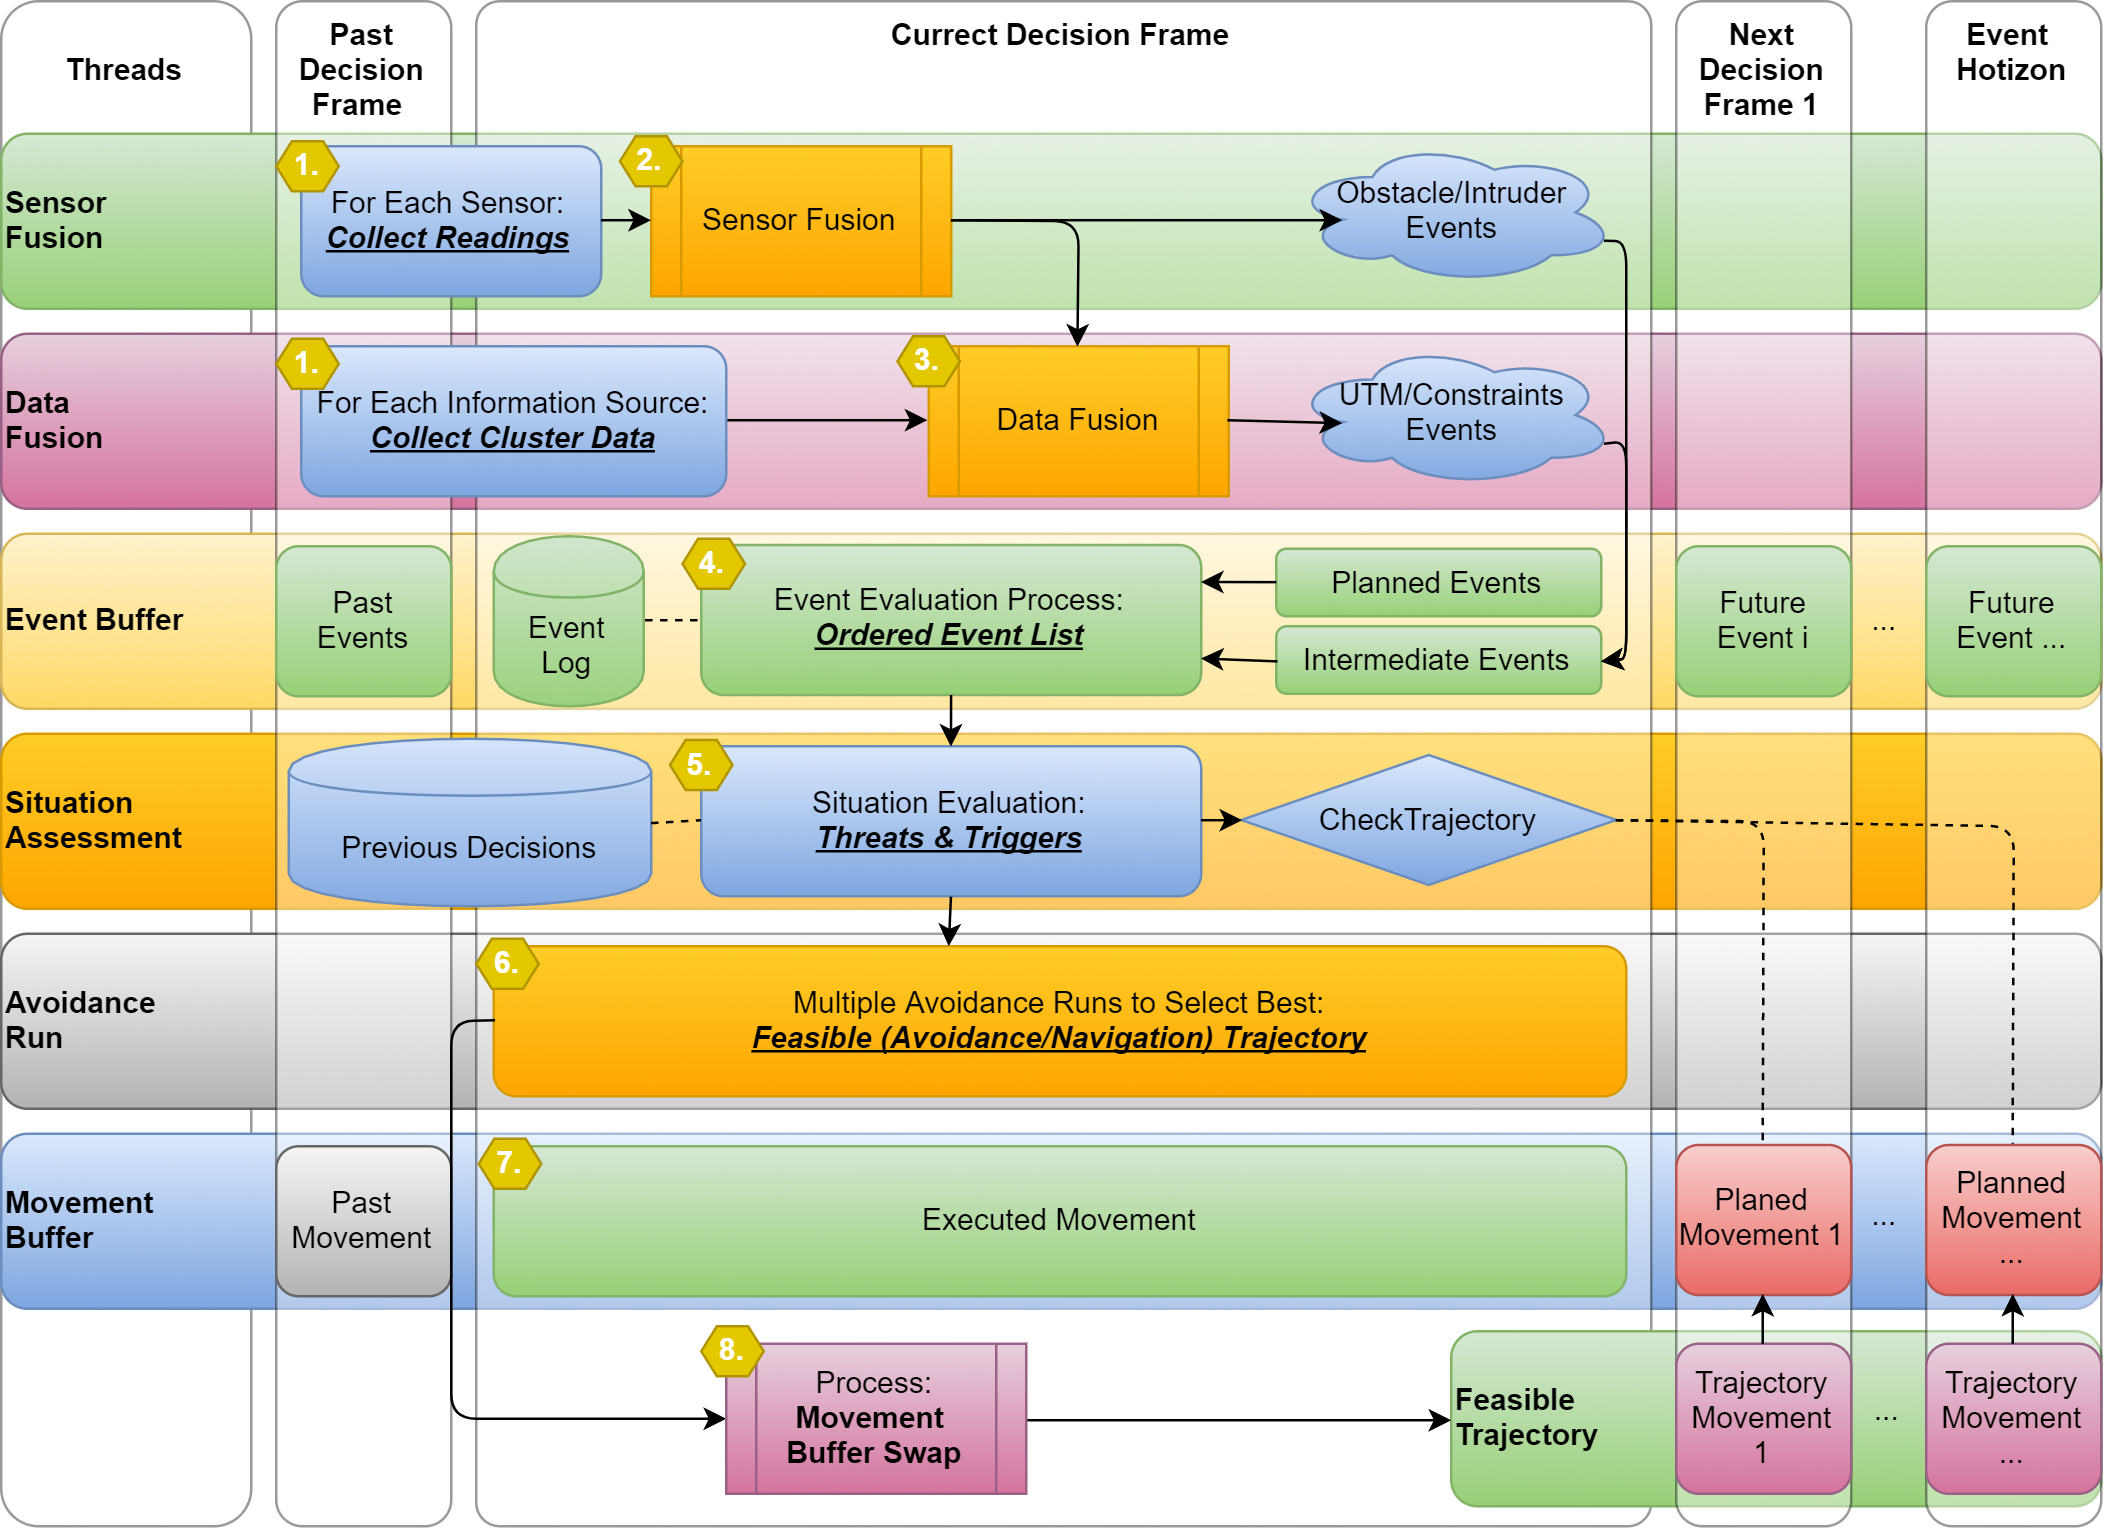
\includegraphics[width=\linewidth]{\FIGDIR/TE064DecisonFrameExplained}
    \caption{Mission control orchestration diagram.}
    \label{fig:misisonControlRunOrchestrationDiagram}
\end{figure}

    \item[3.] \emph{Event Buffer} -  special data structure to store, raise, handle, prioritize events raised by other threads. 
    
    The \emph{implemented events} are listed in 5\textsuperscript{th}-6\textsuperscript{th} step of \emph{mission control run}. The events can be categorized like follow:
    \begin{itemize}
        \item[a.] \emph{Planned events} - raised in previous decision frames to be executed in actual or future \emph{decision frame}. 
        
        \item[b.] \emph{Intermediate events} - raised in \emph{actual decision frame} by other threads to be solved intermediate. 
    \end{itemize}
    
    The event buffer thread executes following event-related activities:
    \begin{itemize}
        \item[a.] \emph{Storing} - the \emph{events} are stored in \emph{event log}. The trace is useful for process and rule fine-tuning. 
        
        \item[b.] \emph{Raising} - the combination of events (multiple avoidance events) (example sec. \ref{s:testRuleMixed}) can trigger additional avoidance behaviour in form of combined-event.
        
        \item[c.] \emph{Handling} - the events are handled by invoking the \emph{situation assessment} or by rule engine invocation (sec. \ref{s:RuleEngineArchitecture}).
        
        \item[d.] \emph{Prioritizing} - the multiple events can be risen during one \emph{decision frame}. Some events cannot be merged and needs to have proper prioritization before handling, like the \emph{obstacle detection} events before \emph{intruder detection event}.
    \end{itemize}
    
    \item[4.] \emph{Situation Assessment} - invoked by \emph{event buffer} o assess situation, responsible for proper \emph{avoidance run} (sec. \ref{s:aviudabceGridRun}) dataset preparation and invocation. The main responsibility is to check \emph{planned trajectory feasibility} stored in \emph{movement buffer} as \emph{planned movements}.
    
    \item[5.] \emph{Avoidance Run} - invoked by \emph{necessity to plan trajectory} originating from \emph{event buffer} or \emph{situation assessment} threads. The avoidance run produces one or multiple \emph{avoidance/navigation} feasible trajectories according to  7\textsuperscript{th}-11\textsuperscript{th} step of \emph{mission control run}.
    
    \item[6.] \emph{Movement Buffer} - represents \emph{movement automaton implementation} (sec. \ref{s:movementAutomatonDefinition}). The movement automaton consumes \emph{movement automaton buffer} each decision frame contains exactly one \emph{movement}. The movements can be viewed as:
    \begin{itemize}
        \item[a.] \emph{Past movements} - already executed movements in \emph{past decision frames}.
        
        \item[b.] \emph{Executed movement} - actually executed movement in current decision frame, this movement cannot be changed.
        
        \item[c.] \emph{Future movements} - future planned movements to be executed after \emph{current decision frame} expires. These movements outlines planned trajectory (predictor mode sec. \ref{s:referenceTrajectoryGenerator}).
    \end{itemize}
    
    \item[7.] \emph{Feasible Trajectory} - consists of \emph{future planned movements} taking place directly after \emph{correct decision frame}. If its necessary, the planned trajectory in movement buffer is no longer feasible, the planned movements will throw away and replaced by \emph{trajectory movements}. 
\end{itemize}

\noindent The \emph{roles \& responsibilities} of each thread have been explained to outline their orchestration and roles in \emph{mission control run} (fig. \ref{fig:missionControlRunActivityDiagram}). The numbered steps in (fig. \ref{fig:misisonControlRunOrchestrationDiagram}) shows the threads orchestration in following manner:

\begin{itemize}
    \item[1.] \emph{Sensor \& Data fusion data set preparation/collection} - the sensor readings are collected through multiple past and over current \emph{decision frame}. Each sensor reading is filtered and processed according to best practices. 
    
    The raw information from various data sources is loaded for relevant space clusters. The relevant space clusters are determined based on \emph{UAS expected position}. 
    
    \item[2.] \emph{Sensor fusion} - the readings from sensors are preprocessed according to (sec. \ref{s:staticObstacles}, \ref{s:intruders}).
    
    \item[3.] \emph{Data fusion} - the information sources are preprocessed according to (sec. \ref{s:staticObstacles}, \ref{s:intruders}).
    
    \item[4.] \emph{Event evaluation process} - the events are evaluated, if there is any triggering event (5\textsuperscript{th}-6\textsuperscript{th} mission control run steps) the situation evaluation process is called.
    
    \item[5.] \emph{Situation evaluation process} - the situation is evaluated according to 5\textsuperscript{th}-6\textsuperscript{th} mission control run steps.
    
    \item[6.] \emph{Feasible trajectory selection process} - from collected \emph{navigation/avoidance trajectories} (7\textsuperscript{th}-10\textsuperscript{th} mission control run steps). If there are more feasible trajectories (increasing threat) the one compliant with the most of the threats is selected.
    
    \item[7.] \emph{Movement execution} - the movement for \emph{current decision frame} is being executed.
    
    \item[8.] \emph{Movement buffer swap} - if there is a new \emph{feasible trajectory} the future movements for next decision frames are flushed away. The movement buffer is then filled with \emph{feasible trajectory movements}.
    \begin{note}
        This step impacts the duration of future \emph{decision frames}.
    \end{note}
\end{itemize}

    	\newpage
\subsection{\secState{R}Computation Complexity}\label{sec:MCRcomputationalComplexity}
\paragraph{Introduction:}The \emph{Computation Complexity} one mission control run assessment is necessary to identify the strong and weak points of approach. Lets get through modules to assess notable calculations/algorithms complexity on high abstraction level.

\paragraph{Navigation Loop:} I the navigation loop, the \emph{waypoint reach condition} (eq. \ref{eq:waypointReachCondition}) is checked, this is unitary operation with worst complexity $\mathscr{O}(1)$. The selection process of the next \emph{Goal Waypoint} can get through all waypoints in the mission if they are all unreachable the complexity is $\mathscr{O}(|waypoints|)$.

The \emph{notable steps} complexity is following:
\begin{equation*}
    \begin{aligned}
        \texttt{Reach Condition: }& \mathscr{O}(1)\\
        \texttt{Select Next Waypoint: }&\mathscr{O}(|waypoints|)
    \end{aligned}
\end{equation*}

\paragraph{Data Fusion:} The \emph{data fusion} is all about \emph{threat selection}. 

If \emph{UAS} is in \emph{controlled airspace} it needs to iterate over received \emph{collision Cases} to select \emph{active ones}. The complexity of this step is linear, therefore boundary is given as $\mathscr{O} (|collision Cases|)$.

Thresholding \emph{Detected Obstacles} is done by simple comparison of \emph{LiDAR ray hits} in given $cell_{i,j,k}$ of \emph{Avoidance Grid}.

Any loading of \emph{threats} from \emph{information sources} is depending on clustering. The \emph{Airspace Clustering} is considered as static for our setup. Therefore the \emph{count of active airspace clusters} has main impact on complexity. The \emph{count of information sources} is static and not changing over mission time. Information sources usually implement \emph{Hash search function} with complexity $\mathscr{O}\ln|searched Item Set|$.

\noindent The \emph{computation complexity} boundaries for \emph{Data fusion} in  our setup are following:
\begin{equation*}
    \begin{aligned}
        \texttt{Select Active Collision Cases: }& \mathscr{O} (|collision Cases|)\\
        \texttt{Threshold Detected Obstacles: }& \mathscr{O}(|cells|)\\
        \texttt{Load Map Obstacles: }& \mathscr{O}(\ln|activeClusters|\times|information Sources|)\\
        \texttt{Load Hard Constraints: }& \mathscr{O}(\ln|activeClusters|\times|information Sources|)\\
        \texttt{Load Soft Constraints: }& \mathscr{O}(\ln|activeClusters|\times|information Sources|)
    \end{aligned}
\end{equation*}

\begin{note}
    The \emph{real-time clustering} is \emph{hard non-polynomial problem} \cite{kleinberg1998microeconomic}.  Usually all information sources and sensor have \emph{polynomial complexity} of processing. The \emph{controlled airspace clusters} are usually set for very long period of time. Therefore \emph{Obstacle Map}, \emph{Airspace Constraints}, and, \emph{Weather Constraints} can be considered as preprocessed
\end{note}

\newpage
\paragraph{Situation Assessment:} The \emph{Situation Assessment} is evaluating triggering events. The \emph{evaluation} is usually simple existence question without further calculations. The \emph{complexity} of \emph{event evaluation} for our case is $\mathscr{O}(1)$. There are 8 triggers. The count of \emph{triggers} needs to be accounted in complexity boundary:

\begin{equation*}
    \mathscr{O}(|triggers|\times event Evaluation Complexity)    
\end{equation*}

\begin{note} The \emph{trigger calculation complexity} needs to stay low, because the \emph{triggers} are verified every \emph{Mission Control Run}. The \emph{Avoidance Run} trigger frequency should be very low under normal conditions.  
\end{note}


\paragraph{Avoidance Run:} The \emph{Avoidance run} is most critical part of \emph{Mission Control Run}, because \emph{Avoidance Path} calculation. The \emph{Navigation Path} calculation is less complex (Rule engine is not accounted), therefore \emph{Emergency Avoidance Mode} is assumed. 

The \emph{threat insertion} is realized in 7\textsuperscript{th} to 10\textsuperscript{th} step. The first is \emph{Avoidance Grid} filled with \emph{Static Obstacles}. The \emph{Avoidance Grid} is designed to separate rotary  \emph{LiDAR} ray space into hit count even cells. Insertion of \emph{LiDAR} scan into \emph{Avoidance Grid} complexity depends on \emph{total cell count}. The \emph{upper boundary} for \emph{insert obstacles} is given like follow:

\begin{equation*}
    \texttt{Insert Obstacles: } \mathscr{O}(|cells|)
\end{equation*}

\noindent The \emph{intruders intersection model} type impact the insertion complexity. The \emph{linear intersection} (sec. \ref{s:linearIntersectionModel}) is going through maximum of \emph{layers count} cells. 

The \emph{body volume intersection model} (sec. \ref{s:bodyvolumeIntersection}) can check the \emph{simple intersection condition} over all \emph{Avoidance Grid} in worst case, therefore complexity for this check is bounded by \emph{count of cells}. 

The \emph{Maneuverability Uncertainty Intersection} (sec. \ref{s:uncertaintyIntersection}) can hit all cells in \emph{Avoidance Grid}. The calculation complexity boundary is exponential depending on \emph{horizontal/vertical} spread in $[rad]$. The \emph{intersection} implementation was done \emph{ad-hoc}. The impact of \emph{intersection application} is visible only when there is more than \emph{4} concurrence intruders (fig. \ref{fig:emergencyHeadOnMultipleComputationTime}).

\noindent The \emph{complexity boundary for \emph{intruder insertion}} is given like follow:

\begin{equation*}
    \texttt{Insert Intruders: }
    \mathscr{O}\left(\sum \begin{bmatrix}
        |linear Intersections| \times |layers|\\
        |body volume Intersections| \times  |cells|\\
        |cells|^{horizontal Spread \times vertical Spread}\\
    \end{bmatrix}\right)
\end{equation*}

\begin{note}
    The \emph{intruder intersection} is critical in \emph{non-controlled airspace}. The main complexity gain in \emph{controlled airspace} is from \emph{rule application}. Our \emph{rule complexity} is in worst case depending on \emph{Reach Set} node count and \emph{Active Collision Cases} count.
    
    \begin{equation*}
        \texttt{Apply Our Rules: } \mathscr{O}(|active Collision Cases| \times |nodes|)
    \end{equation*}
\end{note}

\newpage\noindent For \emph{Hard/Soft Constraints} The algorithm used for intersection polygons was selected based on study \citep{bentley1979algorithms}, the selected algorithm  \emph{Shamos-Hoey} \cite{shamos1976geometric}. The \emph{calculation complexity} boundary is given like follow:

\begin{multline*}
    \texttt{Hard Constraints Intersection:}\\ \mathscr{O}(|cells|\times|hard Constraints| \times \max |constraint Points|^2)
\end{multline*}
\begin{multline*}
    \texttt{Soft Constraints Intersection:}\\ \mathscr{O}(|cells|\times|soft Constraints| \times \max |constraint Points|^2)
\end{multline*}

\noindent Each \emph{threat} category application in \emph{Mission Control Run} is done after \emph{each intersection} in 7\textsuperscript{th} to 10\textsuperscript{th} step. All ratings (tab. \ref{tab:defuzificationRatings}) expect $Reachibility(cell_{ij,k})$ and $Reachibility(Trajectory)$  are calculated. The \emph{calculation complexity} boundary for one \emph{reachibility rating} is $\mathscr{O}(1)$. (eq. \ref{eq:trajectoryReachibility}, \ref{eq:cellReachibility}). The \emph{Recalculate Reachibility} operation applied $4\times$ have maximal \emph{complexity} boundary given as follow:

\begin{equation*}
    \texttt{Recalculate Reachibility: } \mathscr{O}(4 \times (|nodes| + |cells|))
\end{equation*}

\noindent Each time at the end of in 7\textsuperscript{th} to 10\textsuperscript{th} step the \emph{Avoidance Path is Selected}. The \emph{Worst Case} (expected) scenario is to \emph{select} four paths for each \emph{treath} application. The algorithm for \emph{best path selection} (alg. \ref{alg:FindBestPathAvoidanceGrid}) iterates over all \emph{cells} in avoidance grid and over all \emph{trajectories} passing through that cell. The complexity boundary for \emph{path selection} is given as follow:

\begin{equation*}
    \texttt{Select Path: } \mathscr{O}\left(4 \times \left(|cells|+\frac{|nodes|}{|cells|}\right)\right)
\end{equation*}


\paragraph{Conclusion:}  Overall approach complexity is \emph{low}. If proper \emph{Information Sources} with efficient clustering and \emph{intersection models for intruders} are used, the approach will stay within \emph{non-polynomial complexity}. 
The average load time for \emph{testing scenarios} is summarized in (tab. \ref{tab:computationLoadStatistics}).

\begin{note}
    The calculation of \emph{Reach Set} is eliminated by pre-calculation for \emph{state range} \cite{gomola2017obstacle}.
\end{note}
    	\subsection{(R) Safety Margin Calculation}\label{s:safetyMarginCalculation}
\paragraph{Safety Margin Determination:} To determine \emph{safety Margin} the \emph{Rule of Thumb} is used:

\begin{equation}
    maximal Body Radius \le safety Margin \le 2 \times turning Radius
\end{equation}

\noindent The \emph{lower boundary} is given by \emph{UAS} construction. because the \emph{UAS} body is considered as \emph{unit ball} with radius given as \emph{maximal body radius}. 

The \emph{upper boundary} is optional, The \emph{double of \emph{turning radius}} is used by the \emph{conservative approach} \cite{borenstein1991vector}.


\paragraph{Safety Margin Bloating:}  The \emph{discretization} of \emph{Reach Set}, \emph{Operation Space} and \emph{Decisions} imposes standard \emph{mixed integer} problem in terms of \emph{safety}. This section covers \emph{non-exhaustive} list of possible \emph{Safety Margin Bloats} in our approach.

\paragraph{Own Position Uncertainty Bloat:} The \emph{sensor fusion} is precise, but not \emph{exact} in own UAS position determination. The maximal usual disparity needs to be accounted into \emph{Safety Margin}.

\paragraph{Intruder Position Uncertainty Bloat:} The \emph{sensor fusion} of Intruder is precise, but not \emph{exact} in own UAS position determination. The maximal usual disparity needs to be accounted into \emph{Safety Margin}.

\paragraph{Weather bloat:} The \emph{Weather} impact type may result to increased \emph{safety margin}. Example: UAS is not humidity resistant, the clouds will be avoided from greater distance.

\paragraph{Airspace bloat:} The \emph{Airspace} depending on cluster or \emph{country} may require greater separation distances, depending on circumstances. The example can be UAS directive to keep minimal separation from obstacles. The \emph{Safety Margin} is usually overridden by UTM directive value.

\paragraph{UTM Synchronization Bloat:} \emph{Both UAS} decision times were \emph{synchronized}. The \emph{intruder} can be offset for \emph{full decision frame}. This is not an assumption, but it shows critical performance. Usually safety margin is bloated for (worst case offset):
\begin{equation}\label{safetyMarginBloat}
    safetyMarginBloat = \left( \begin{aligned}
    &intruderVelocity \times\dots \\ &intruderDecisionFrame \end{aligned}\right)[m,ms^{-1},s]
\end{equation}
    
    %06-08 UTM implementation
		\cleardoublepage
\section{UTM Prototype Implementation}\label{sec:UASTrafficManagement}

\noindent The \emph{Traffic Management} for UAS is based on existing Air Traffic Management System for manned aviation \cite{icao4444}. The controlled airspace segments are \emph{static} and have one \emph{authority for one zone} principle. The dynamic zones have been proposed in \cite{gerdes2016dynamic}. However, it will be omitted for \emph{simplification purpose}. The necessity for \emph{UAS integration} into \emph{National Airspace} has been outlined in \cite{spriesterbach2013unmanned}.

The latest \emph{Airbus blueprint} \cite{airbusUTM2018blueprint} outlines some functionality. The main purpose of this section is to show \emph{Reach Set based Approach} capability to follow \emph{Usual Air Traffic Management} commands.

The \emph{section} is organized to introduce:
\begin{enumerate}
    \item \emph{UTM Architecture} (sec. \ref{sec:utmArchitecture}) - centralized ATM-like authority over airspace cluster.
    
    \item \emph{Handling Standard Collision Situations} - head-on approach (sec. \ref{sec:handlingHeadOnApproach}), converging situation (sec. \ref{sec:handlingConvergingManuever}), overtake (sec. \ref{sec:handlingOvertakeManuever}).
    
    \item \emph{Position Notification} (sec. \ref{sec:positionNotification}) - position notification design.
    
    \item \emph{Collision Case} (sec. \ref{sec:collisionCase}) - calculation and handling of \emph{collision situations}.
    
\end{enumerate}

\noindent The additional material can be found in:
\begin{enumerate}
	\item \emph{Cooperative Conflict Resolution} (app. \ref{sec:cooperativeConflictResolution}) - the model used for conflict resolution in \emph{controlled airspace}.
    
    \item \emph{Non-Cooperative Conflict Resolution} (app. \ref{sec:nonCooperativeConflictResolution})  - the model used for conflict resolution in \emph{non-controlled} airspace and \emph{emergency avoidance}.
    
    \item \emph{Weather Case} (app. \ref{sec:weatherCase}) - definition and handling of \emph{weather hazards}.
\end{enumerate}
		\subsection{(R) Architecture}
\paragraph{UTM concept} is based on \emph{asynchronous event-based control} \cite{zimmer2011rule}. \emph{Event} in \emph{controlled airspace} is handled in form of \emph{cases} \cite{prevot2016uas}. There are following \emph{event sources}:

\begin{enumerate}
    \item \emph{Weather Information Service} (from \cite{zimmer2014selective}) - used to create \emph{weather case} (tab. \ref{tab:weatherConstraint}).
    
    \item \emph{Position Notification from UAS systems} (tab. \ref{tab:positionNotification}) - used to create \emph{collision cases} (new functionality) (tab. \ref{tab:collisionCase}).
\end{enumerate}


\paragraph{Decision frame} (eq. \ref{eq:decisionFrameDefinition}). The \emph{UTM} is operating in discrete decision frames which are starting on current \emph{decision time} and ending at  next \emph{decision  time}:

\begin{equation}\label{eq:decisionFrameDefinition}
    decision Frame_i = [decision Time_i, decision Time_{i+1}[,\quad i \in {1,\dots,k}, k \in \N^+
\end{equation}

\paragraph{Event based airspace control} is collecting  events in  previous $decisionFrame_{i-1}$ and issuing commands in current $decisionFrame_i$.There are following phases during the \emph{UTM frame} cycle:
\begin{enumerate}
    \item \emph{Planning} - the detection phase, when the hazardous situations are assessed.
    
    \item \emph{Fulfillment} - the monitoring phase, when the state of affairs for directives and mandates is full filled by controlled UAS systems. 
    
    \item \emph{Acknowledgement} - the closing phase, when UTM assess and acknowledges the performance of controlled UAS systems.
\end{enumerate}


\begin{figure}[H]
    \centering
    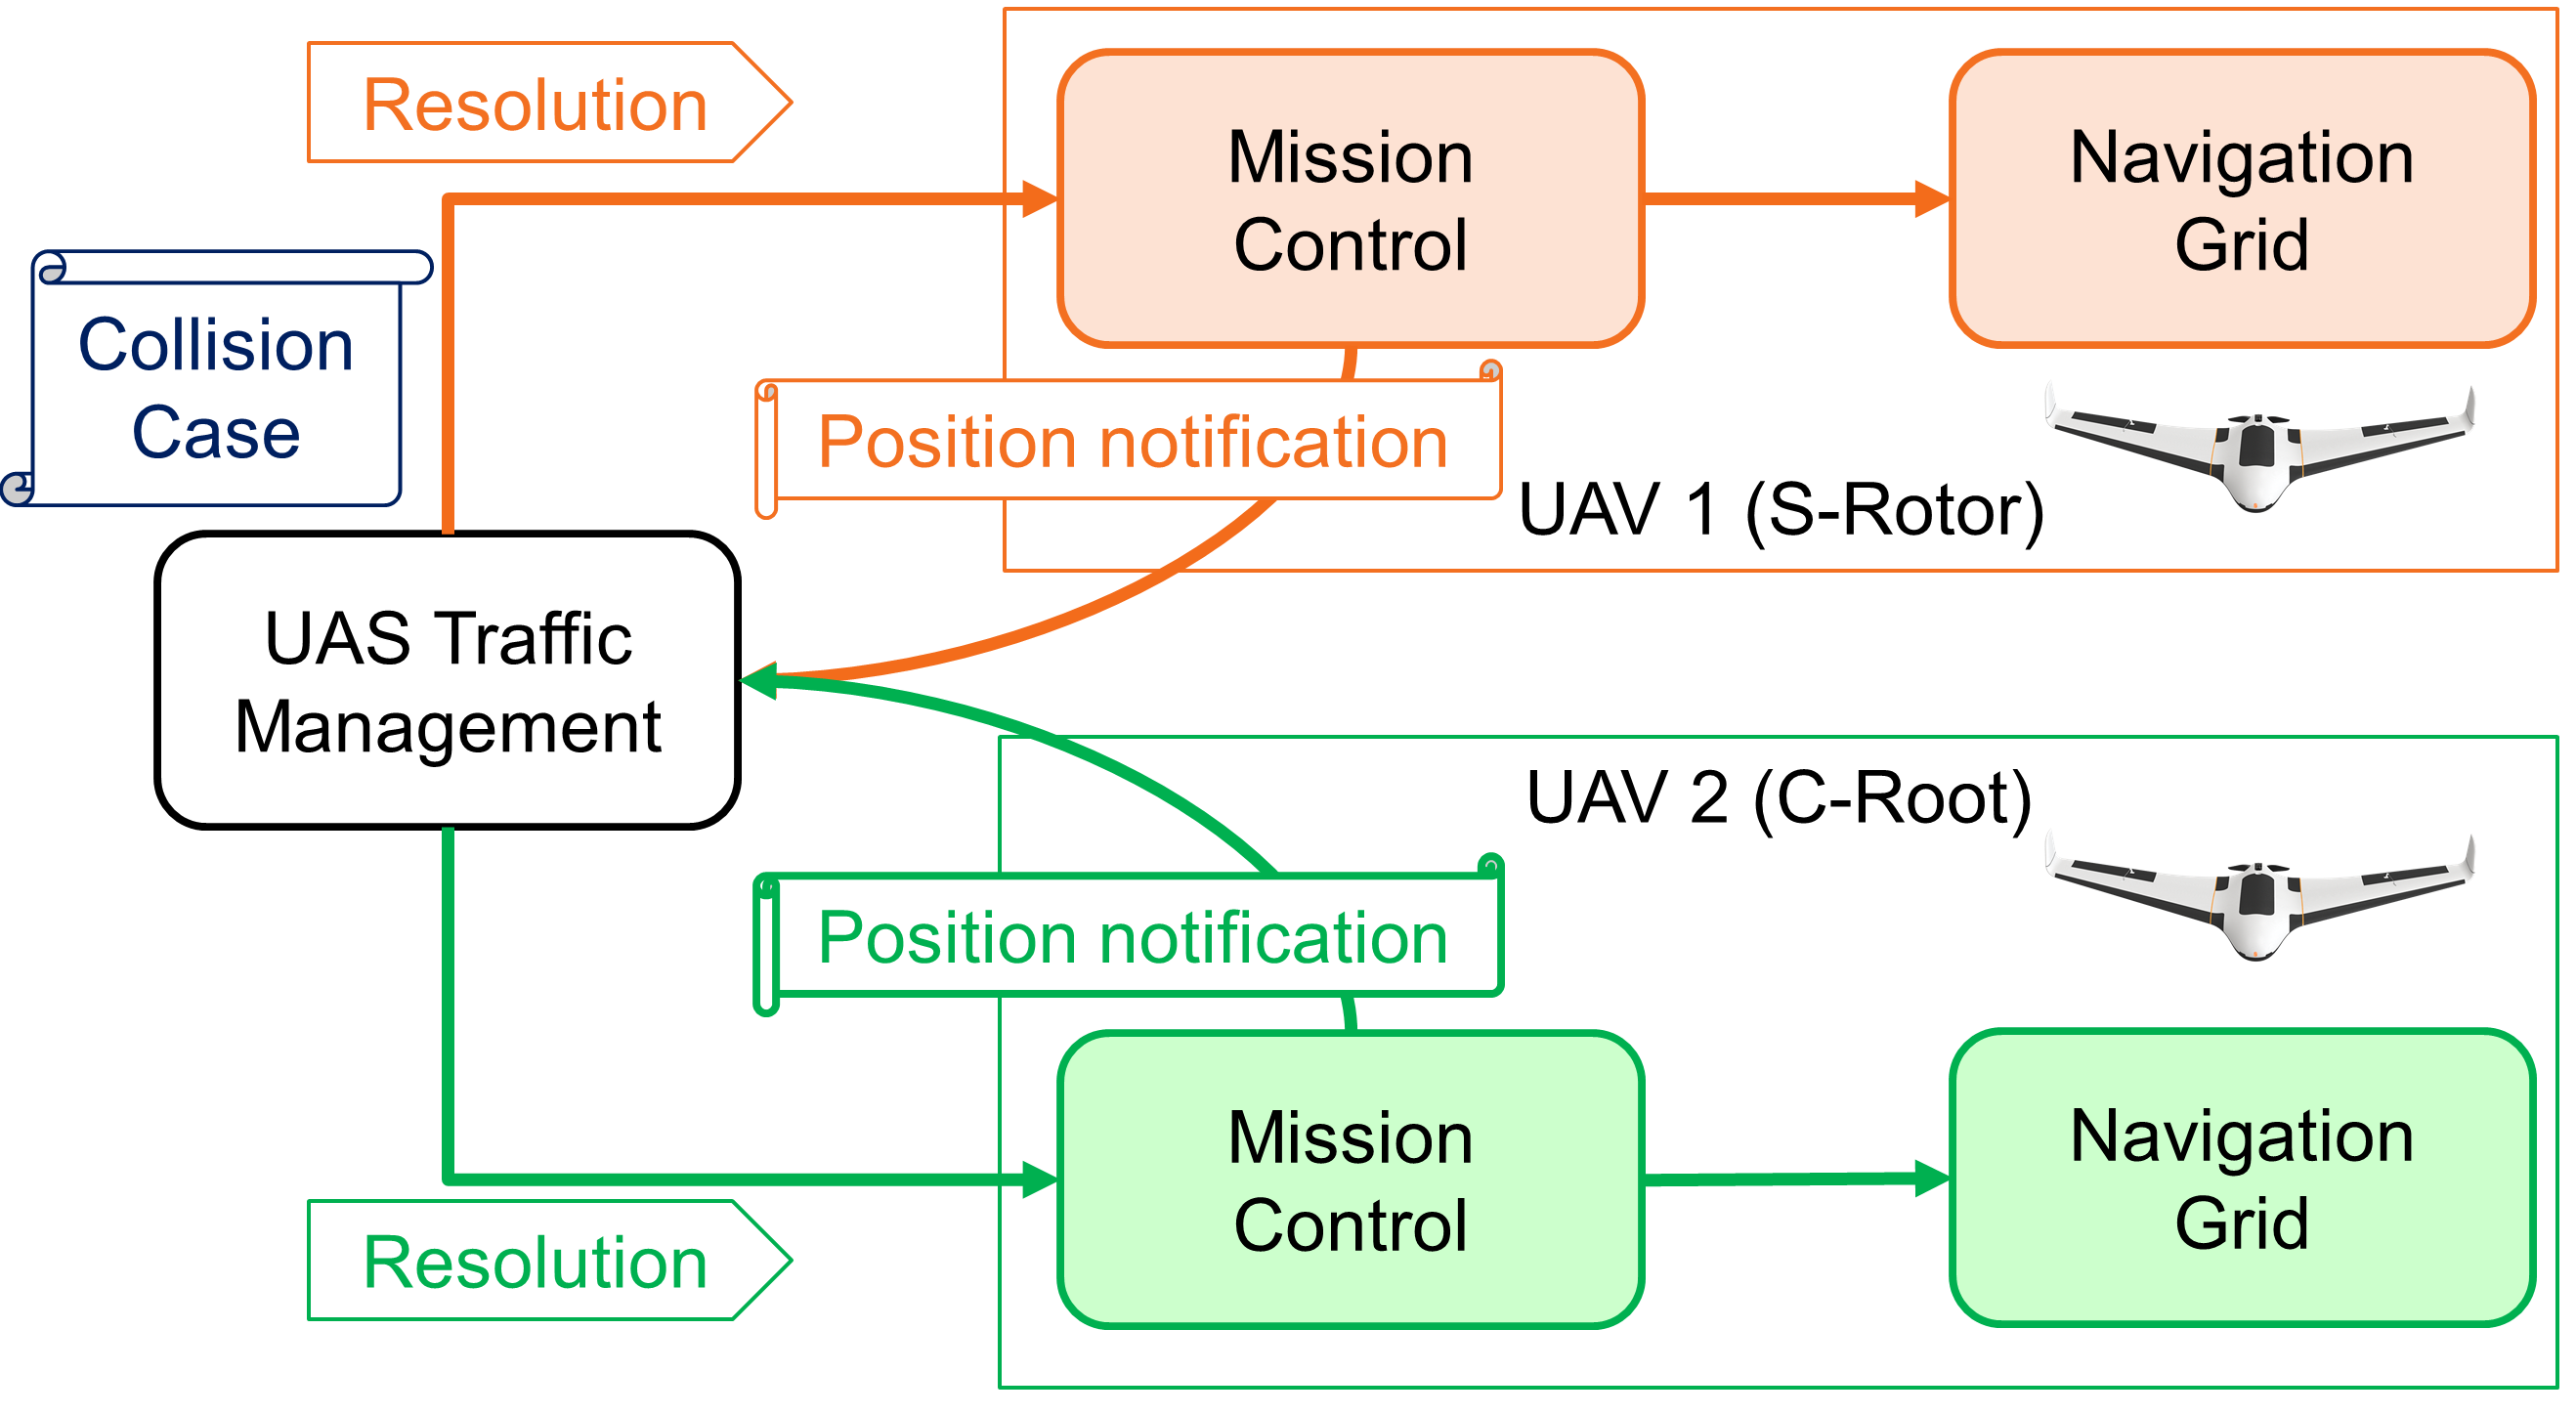
\includegraphics[width=0.7\linewidth]{\FIGDIR/RE002UTMCommunicationDiagram} 
    \caption{UAS Traffic (UTM) Management architecture overview.}
    \label{fig:UTMArchitectureOverview}
\end{figure}

\paragraph{Architecture:} (fig. \ref{fig:UTMArchitectureOverview}).  There are multiple UAS systems equipped with standard \emph{Mission Control} and \emph{Navigation} procedures. 

Depending on the \emph{airspace cluster} decision time frame they are sending \emph{periodical position notifications} (tab. \ref{tab:positionNotification}).

The \emph{UAS Traffic Management} (UTM) collects the event data from \emph{Weather Information Service} and \emph{Position Notifications} calculating respective \emph{cases}. 

If there is an \emph{active collision/weather case} the \emph{UTM} will send \emph{resolutions} to respective airspace attendants. 
		\subsection{(R) Cooperative Conflict Resolution}\label{sec:cooperativeConflictResolution}


\paragraph{Idea:} There is a \emph{final decision maker} (absolute authority) in conflict resolution. This authority is \emph{UTM} or \emph{air traffic attendant} with higher priority. The future \emph{UTM system} is such authority. The approach to mixed conflict resolution is mentioned in \cite{ramasamy2014towards}, based on navigation \cite{ramasamy2013novel}. This is similar to our approach. 

\begin{note}
    \emph{Open Issue:} Decentralized model with UTM as approver of directives is possible, but that is topic for own research.
\end{note}

\paragraph{Goal:} UAS is obligated to follow up committed mission plan with given precision.  There is one to five percent  allowed deviations for ATM mission plans.     Similar rates are achievable according to \cite{ramasamy2014towards}.  This requirement is given by \cite{icao4444} ICAO 4444 document for ATM operations.

\begin{figure}[H]
    \centering
    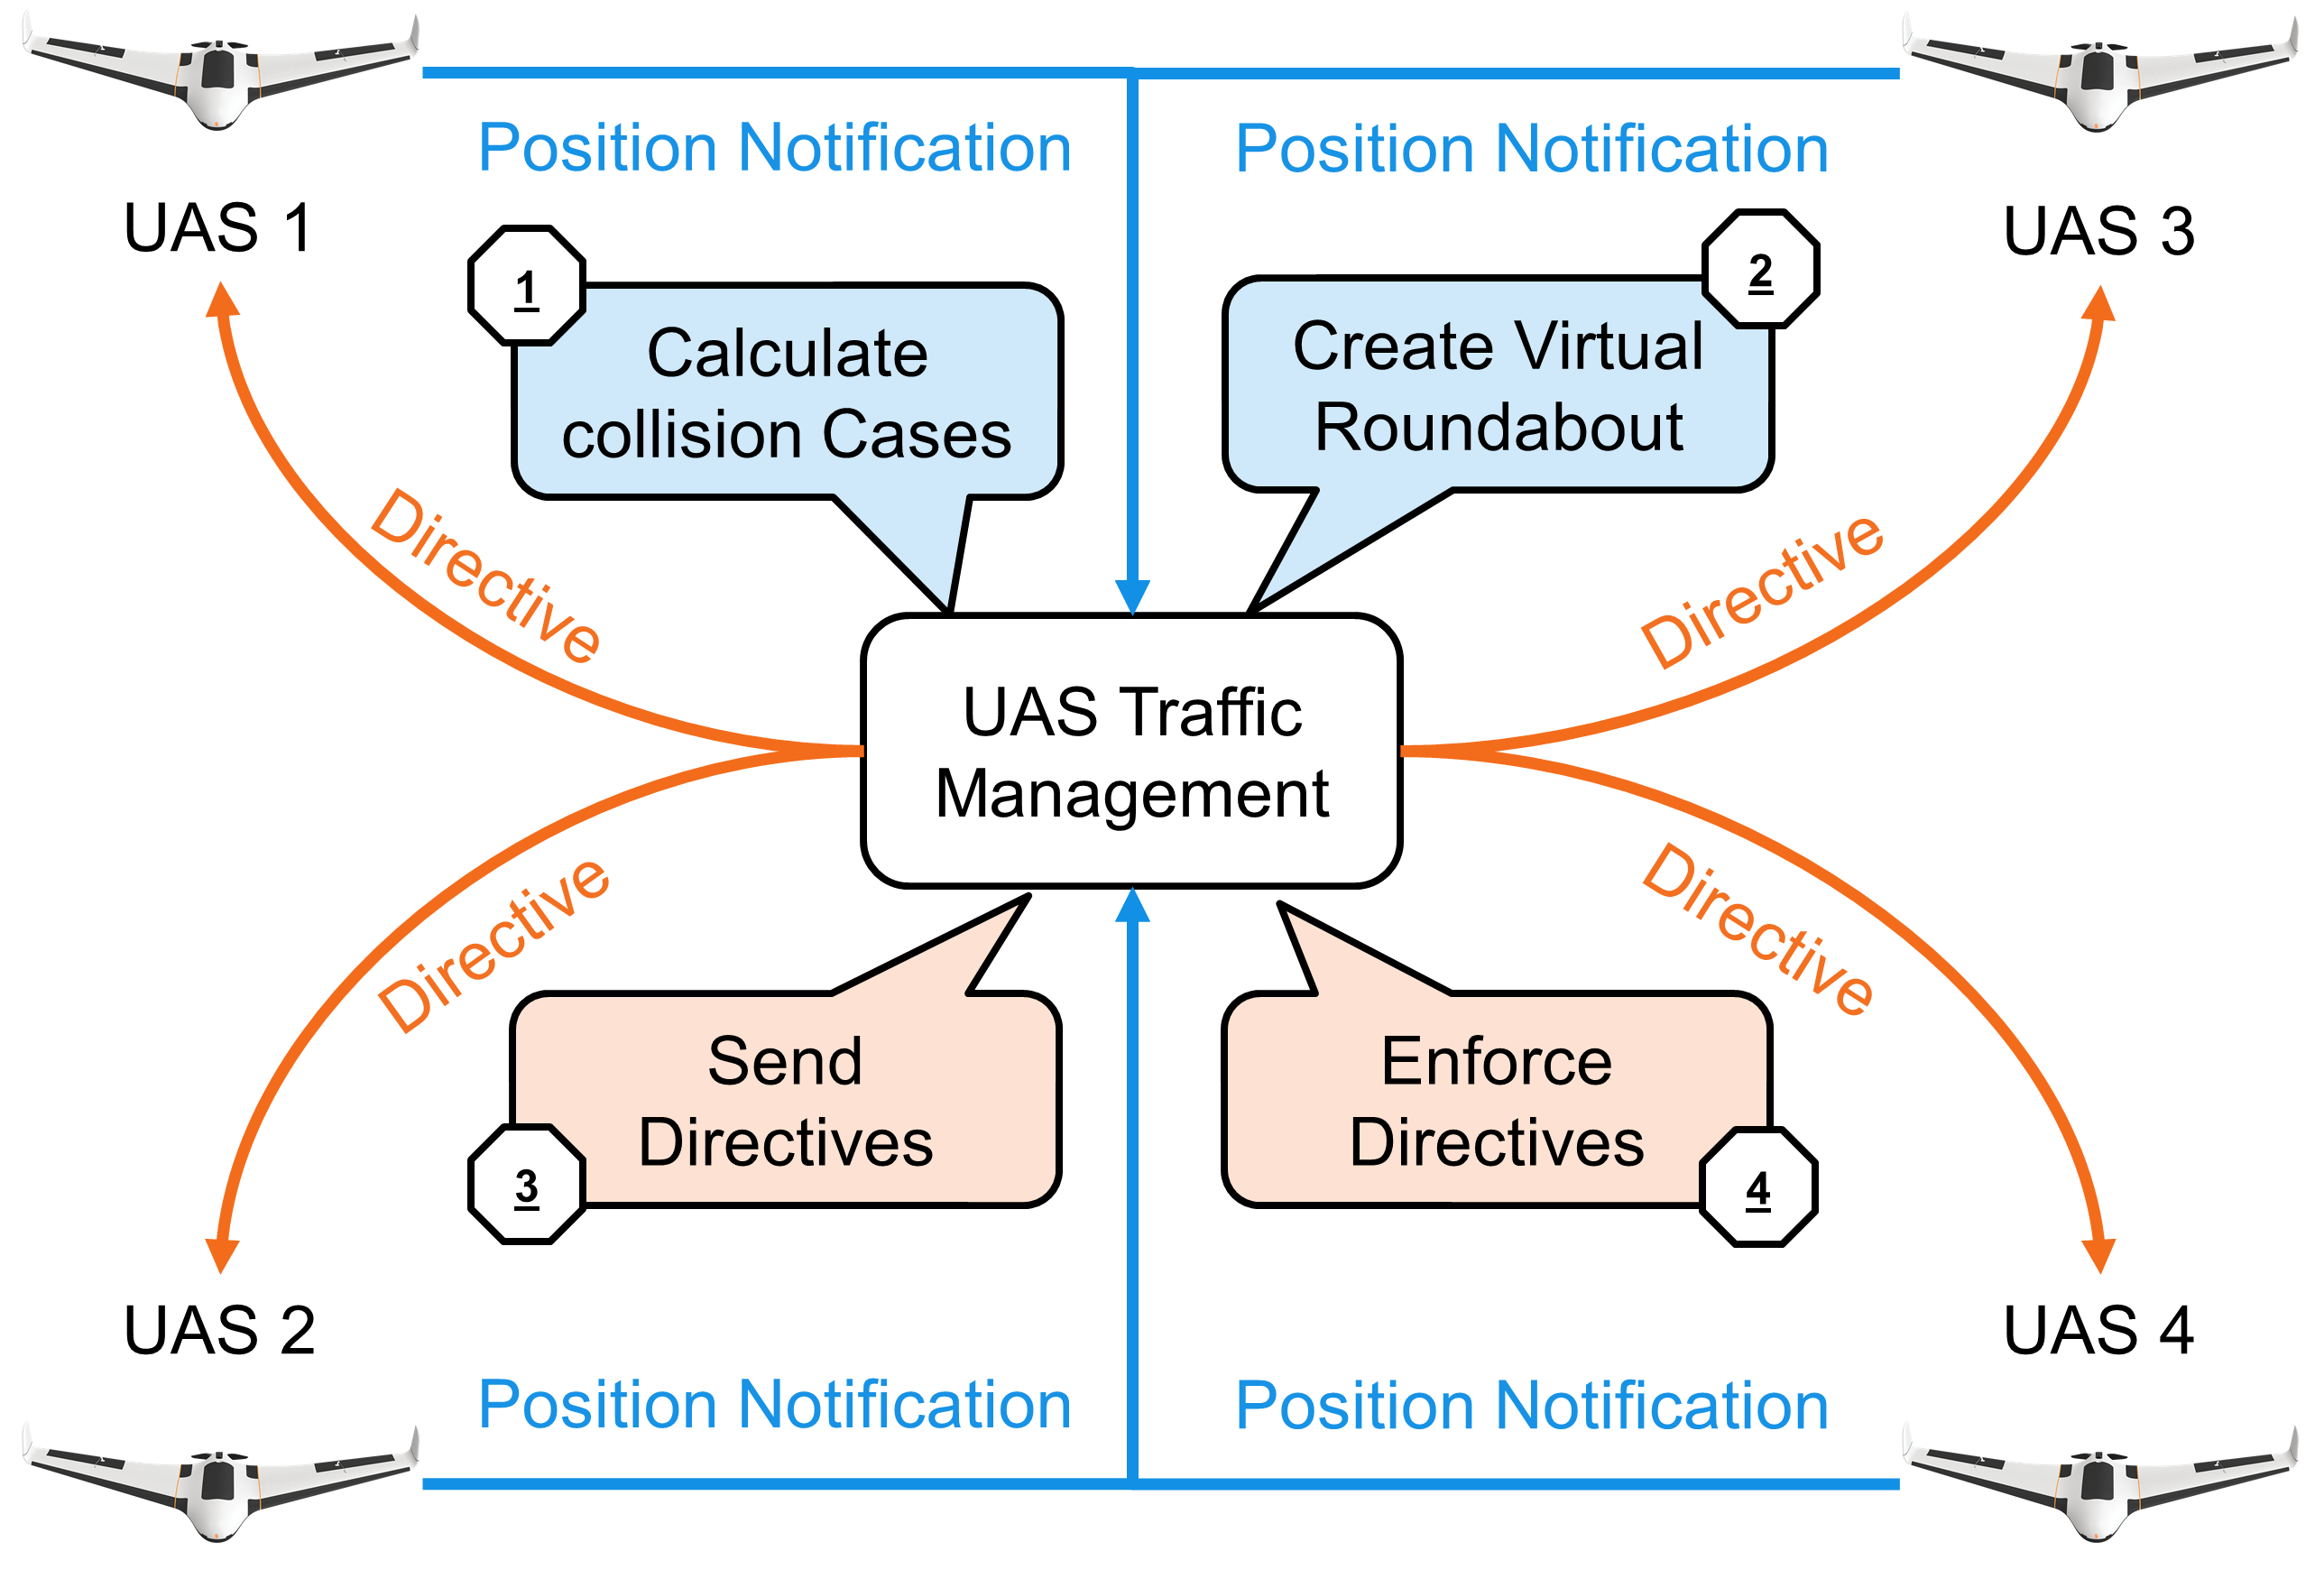
\includegraphics[width=0.7\linewidth]{\FIGDIR/RE003CooperativeResolution} 
    \caption{Cooperative conflict resolution via UTM authority.}
    \label{fig:CooperativeConflictResolutionUTM}
\end{figure}

\paragraph{Cooperative conflict resolution} (fig. \ref{fig:CooperativeConflictResolutionUTM}) shows functional diagram of one \emph{UTM time-frame} there  are following actors:
\begin{enumerate}
    \item \emph{Unmanned Autonomous System} (UAS) equipped with necessary navigation and communication modules, providing the unique \emph{identification number}.
    
    \item \emph{UAS Traffic Management} (UTM) posing as central authority for given \emph{airspace cluster}.
\end{enumerate}

\noindent The following steps are executed during \emph{Cooperative conflict resolution}:
\begin{enumerate}
    \item $UAS_* \to UTM$ \emph{Send position notification} - each \emph{UAS} is notifying the authority (UTM)
    
    \item $\circlearrowright UTM$ \emph{Calculate collision Cases} - UTM gathers data and predicts possible collisions then it tries to link them and manage the situation.
    
    \item $\circlearrowright UTM$ \emph{Create virtual Roundabout} - active collision cases are aggregated into virtual roundabout. 
    
    \item $UTM \to UAS_*$ \emph{Send directives} - UTM sends commands to UAS systems whom needs to change their planned trajectories. 
    
    \item $UTM \to UAS_*$ \emph{Enforce directives} - UTM is periodically checking constraints imposed in previous \emph{decision frames}.
\end{enumerate}
		\subsection{\secState{R}Non-Cooperative Conflict Resolution}\label{sec:nonCooperativeConflictResolution}

\paragraph{Idea:} There is \emph{main UAS(1)} which is flying in open \emph{non-controlled} airspace. Other UAS are operating in its vicinity. It is expected that they are claiming their \emph{planned trajectories}. The \emph{Main UAS(1)} detects the collision with other \emph{UAS}(2-4).

There is no \emph{final decision maker} nor \emph{supervising authority}; all communication participants have a similar level of rights. 
\begin{note}
    There is an assumption that other airspace users are behaving like intruders, without intent to destroy or harm. The \emph{adversarial behavior} is not accounted. The response from an \emph{intruder} is not mandatory in \emph{non-controlled} airspace.
\end{note}

\paragraph{Goal:} Provide \emph{mutual avoidance mechanism} in \emph{non-controlled} airspace. Let us consider the equal standpoint of all airspace attendants.

\paragraph{Conflict Resolution:} The conflict resolution depends on current mode and \emph{handshake} between airspace attendants. The non-cooperative behavior has been implemented as follows:

\begin{enumerate}
    \item\emph{Navigation mode} - every \emph{airspace attendant} is calculating own \emph{collision cases} and checking the behavior of the other (virtual UTM).
    
    \item\emph{Emergency avoidance mode} - is depending on communication mode:
    \begin{enumerate}[a]
        \item\emph{Response mode} - claiming separation methods and using avoidance mechanism (Avoidance grid with intruder model in our case).
        
        \item\emph{Blind mode} - every conflict side picks own strategy respecting given \emph{rules of the air}.
    \end{enumerate}
\end{enumerate}

\begin{note}
    \emph{Intruder Intersection model selection:} UAS based on Event detects possible collision for some reason UTM directive is out of the question, then try to claim separation (body volume intruder model (app. \ref{s:bodyvolumeIntersection})), If separation fails, go full survival mode (uncertain intruder model (app. \ref{s:bodyvolumeIntersection})).
\end{note}

\newpage \paragraph{Special Cases in Manned Aviation:} There are IFALPA reports which can give us an overview of \emph{enforced non-cooperative} mode causes in \emph{controlled airspace}:  
\begin{enumerate}
    \item \emph{VFR disabled} - flying in fog or thick clouds can render pilot vision, similar to UAS cameras/LiDAR.
    
    \item \emph{IFR equipment broke} - the sensor malfunction is more likely to happen due to the lesser redundancy in UAS systems.
    
    \item \emph{C2C Link disabled} - communication loss is more likely to happen, due to the lesser redundancy.
    
    \item \emph{ATM failure} - the ground control module of UTM can also fail.
\end{enumerate}

\begin{note}
    Traffic management related fails are lesser than 0.001 cases per one flight (according to IFALPA \cite{subotic2007recovery}).
\end{note}

\begin{figure}[H]
    \centering
    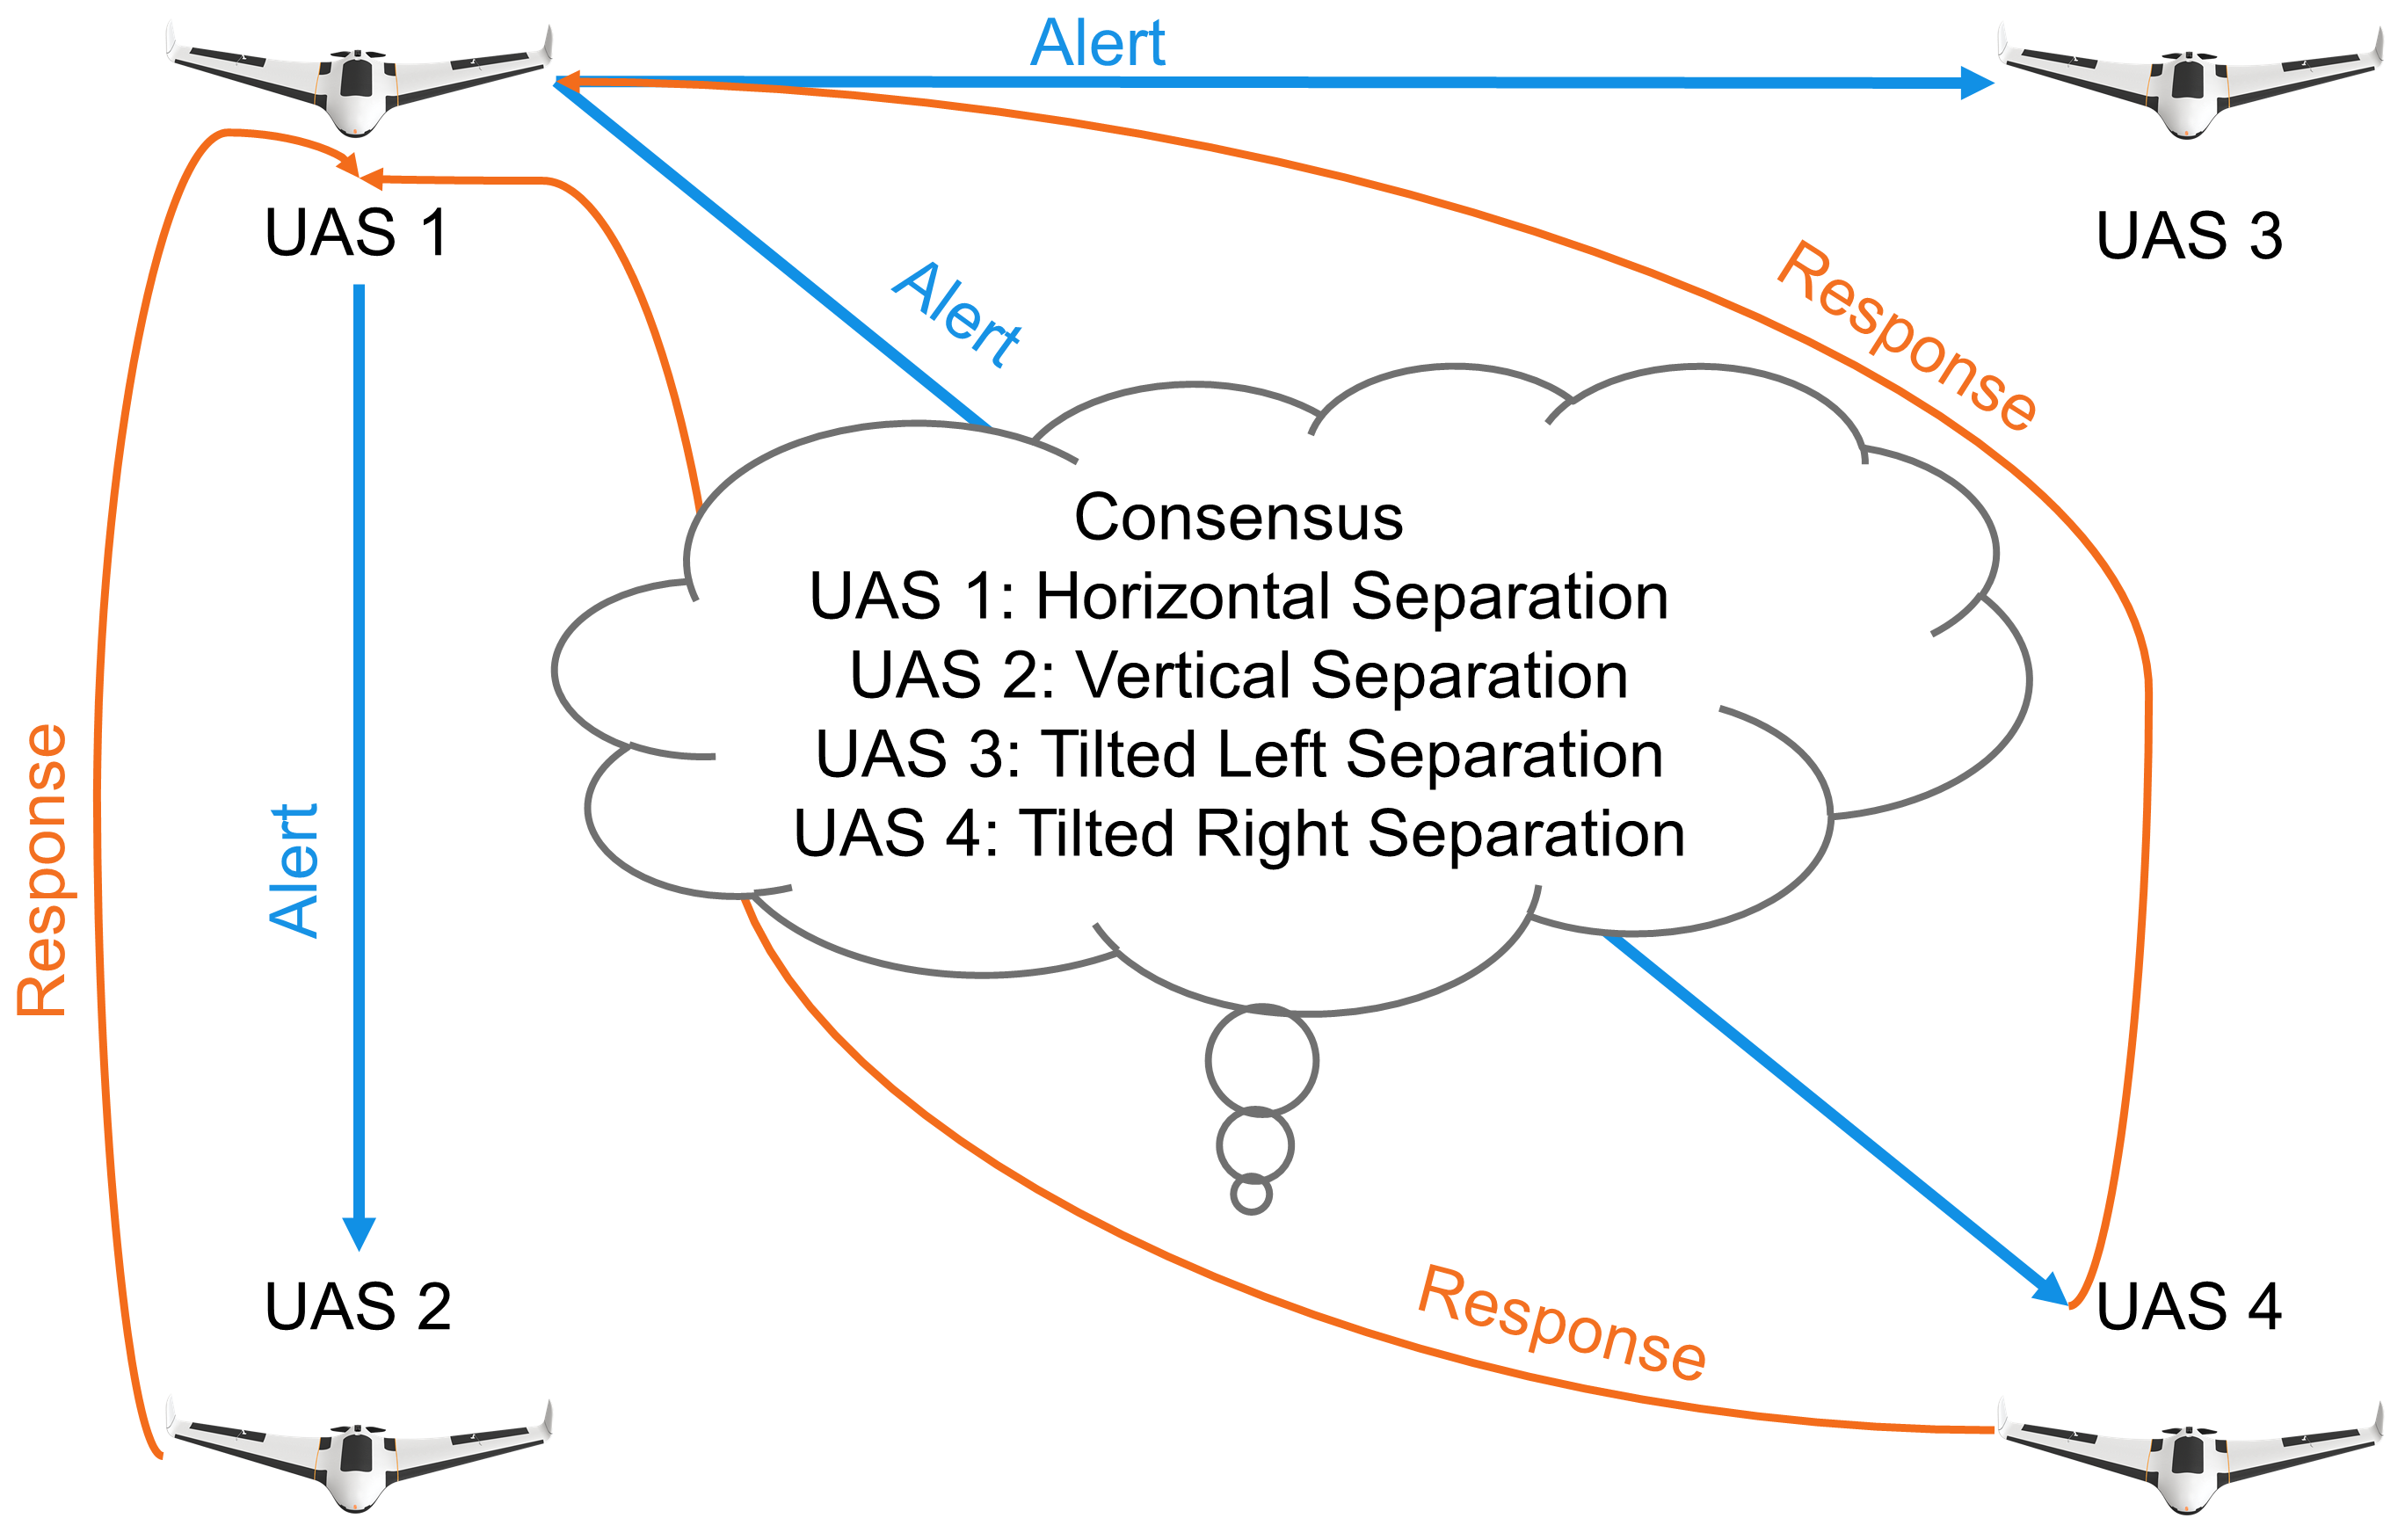
\includegraphics[width=0.7\linewidth]{\FIGDIR/RE004NonCooperativeResolution} 
    \caption{Non-cooperative conflict resolution via UAS claims.}
    \label{fig:NonCooperativeConflictResolutionUTM}
\end{figure}

\paragraph{Response mode scenario example:} The \emph{main UAS(1)} is going to collide with other \emph{UAS}(2-4):
\begin{enumerate}
    \item $UAS(1) \to UAS(2-4)$ sends position and heading notification.
    \item $\circlearrowright UAS(2-4)$ calculates possible collisions.
    \item $UAS(2-4) \to UAS(1)$ sends a response to the \emph{main UAS(1)} with claimed separation mode. 
    \item $\circlearrowright UAS(1)$ acknowledges proposed \emph{separation modes}.
    \item $\circlearrowright UAS(1-4)$ avoids each other using claimed separation mode because every \emph{UAS} achieved \emph{consensus}.
\end{enumerate}

\begin{note}
	The mutual consensus is not usually achieved via C2 communication. The most common case is \emph{assuming separation mode}. This case is shown in (sec. \ref{s:testEmergencyMixed})
\end{note}
		\subsection{Handling Head-on Approach}\label{sec:handlingHeadOnApproach}

\paragraph{Summary:} Two UAS are facing each other head-on. There is a need to define triggers for detection and resolution approach for autonomous UAS.  Rules for VFR/IFR modes in manned aviation are the base for the autonomous collision resolution. The concept of the virtual roundabout is introduced.

\paragraph{Goal:} Identify required parameters sufficient for automatic solution of \emph{Head-on collision} situation.

\paragraph{VFR:} The \emph{Visual Flight Rules} (VFR) are specified in annex 2 \cite{icaoAnnex2}, and there is a \emph{Head-on} approach for two or more air crafts. The definition is rather vague: "The pilot should diverge from original heading to the right to create sufficient, safe space for avoidance." 

\paragraph{IFR:} The \emph{Instrument Flight Rules} in annex 2. \cite{icaoAnnex2} and 11. \cite{icaoAnnex11} are defining the boundaries and events for success full \emph{Head-on resolution} in larger detail. 

The parameter values are useless due to the UAS scaling factor; the following parameters can be used in UTM:

\begin{enumerate}
    \item The \emph{angle of approach $\ge 130^\circ$} - the minimal planar angle between aircraft positions and expected collision point is in the interval $[130^\circ,180^\circ]$.
    
    \item \emph{Minimal detection range} - the minimal detection range of head-on collision is $2\times turning Radius + safety Margin$.
    
    \item \emph{Safety margin} - during avoidance all aircraft keeps mutual distance at least the value of safety margin.
\end{enumerate}

\begin{figure}[H]
	\centering
    \begin{subfigure}{0.45\textwidth}
    	\centering
        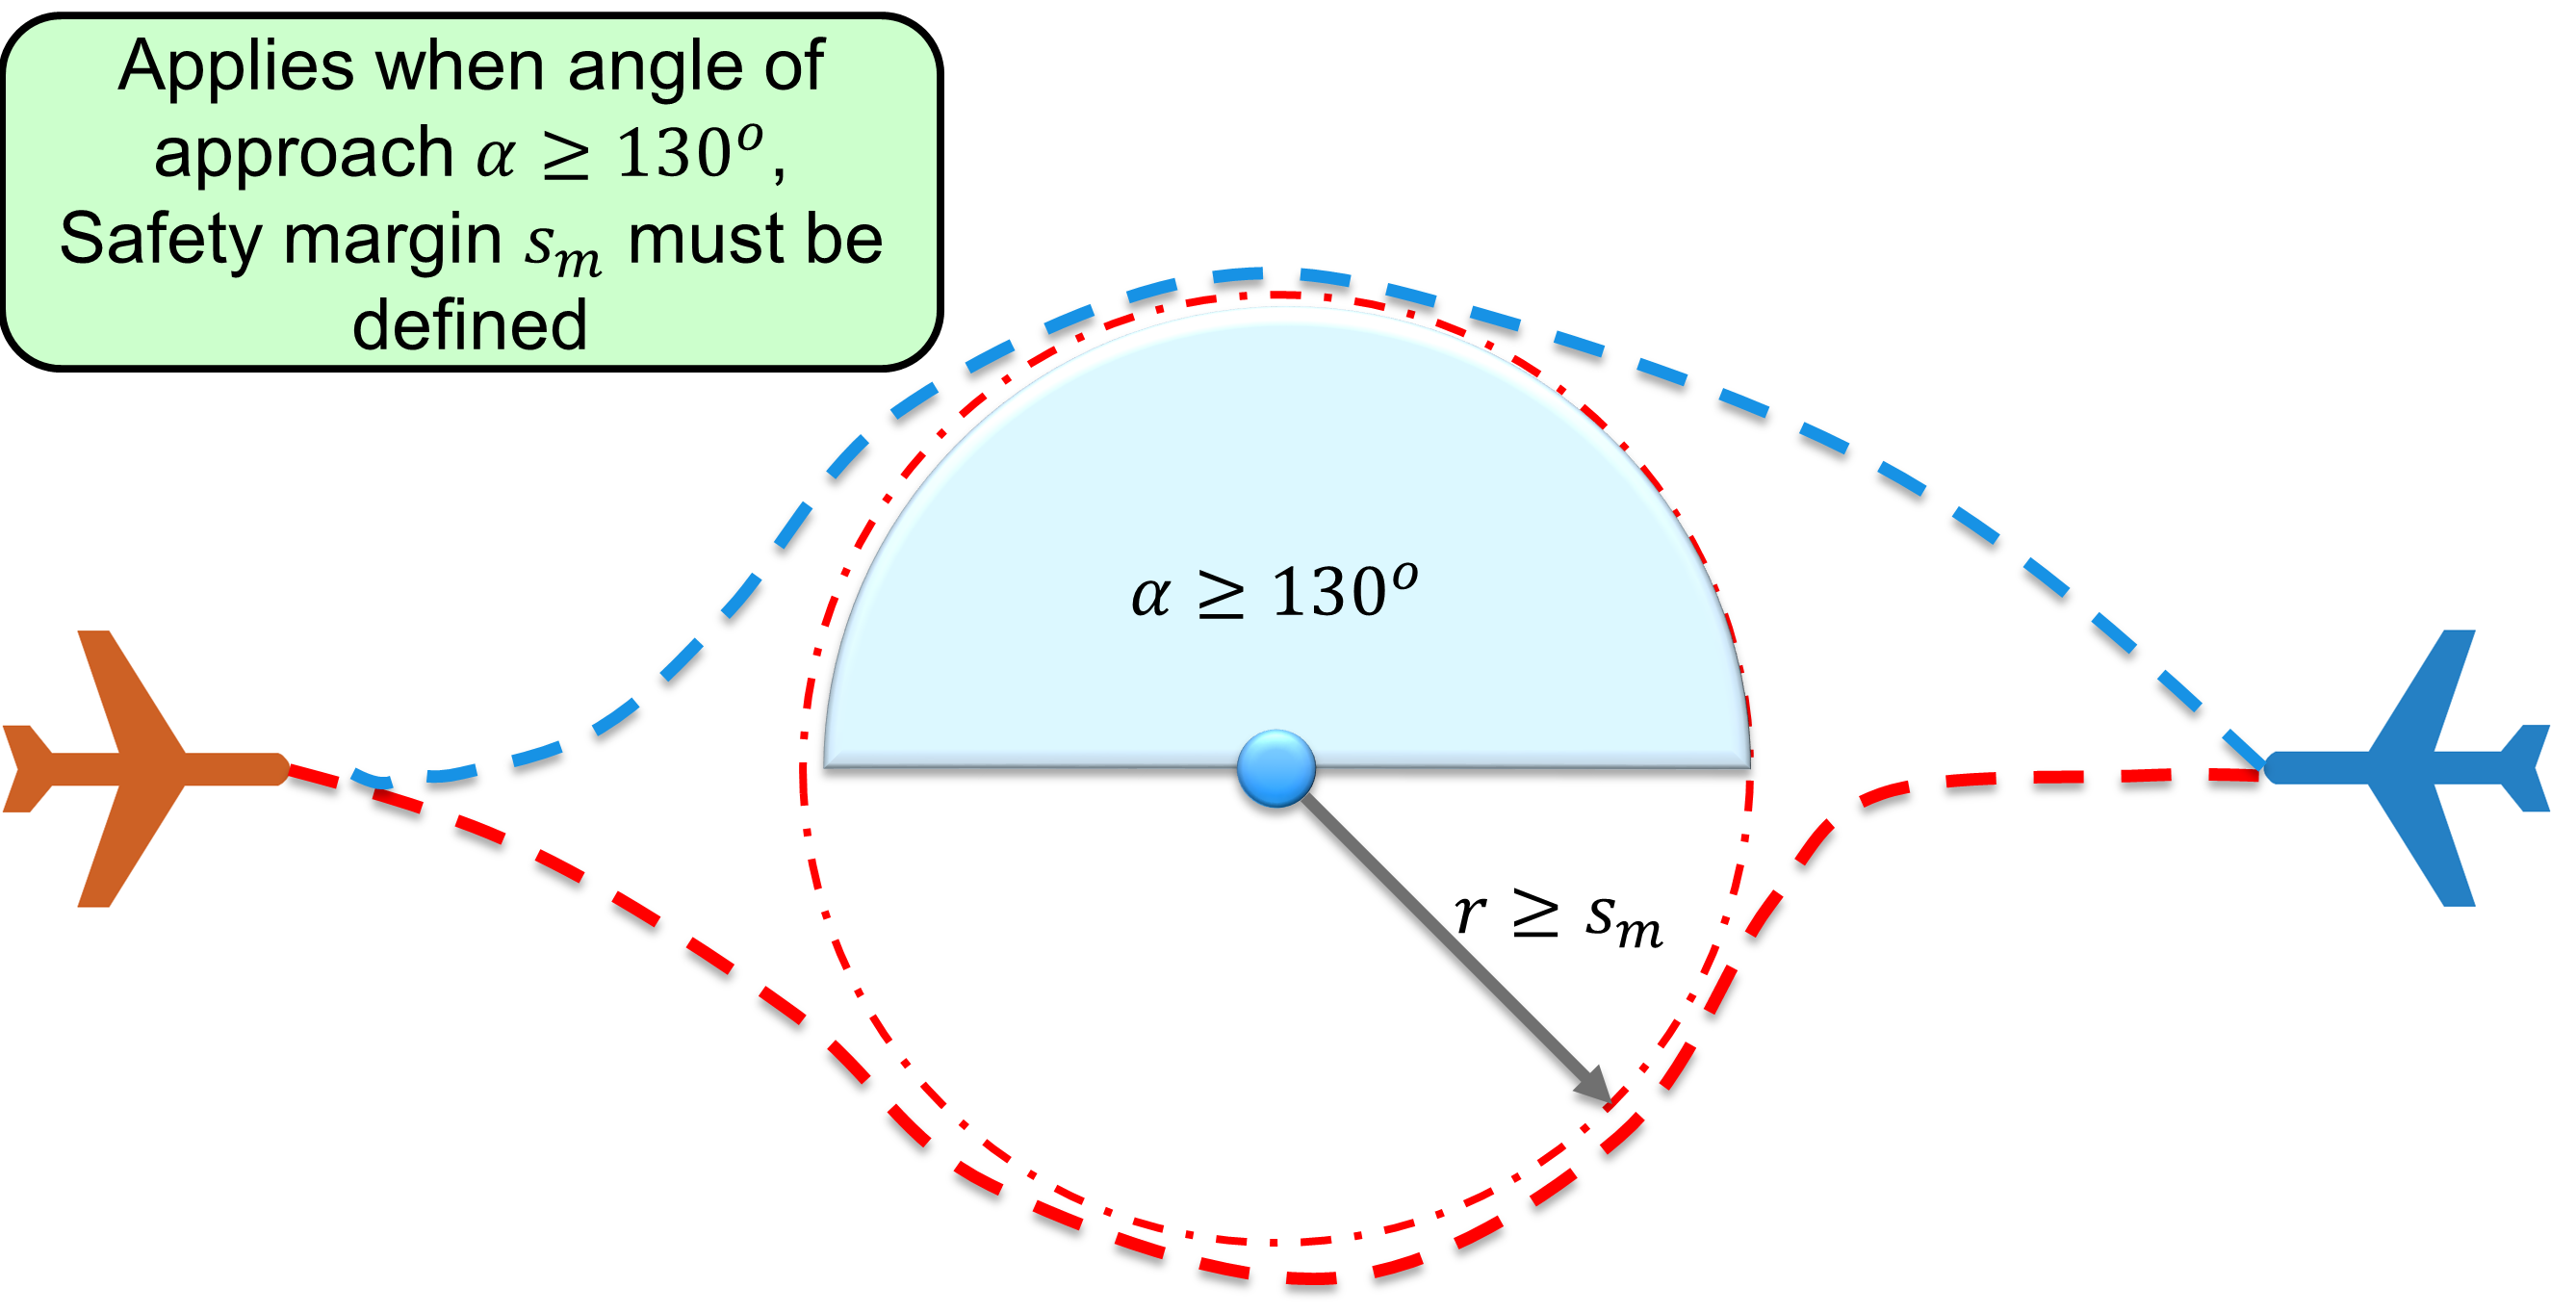
\includegraphics[width=0.9\linewidth,height=95pt,keepaspectratio]{\FIGDIR/RE008HeadOnApproach01} 
        \caption{Detection.}
        \label{fig:HeadOnApproachTheoreticalDetection}
    \end{subfigure}
    \begin{subfigure}{0.45\textwidth}
    	\centering
        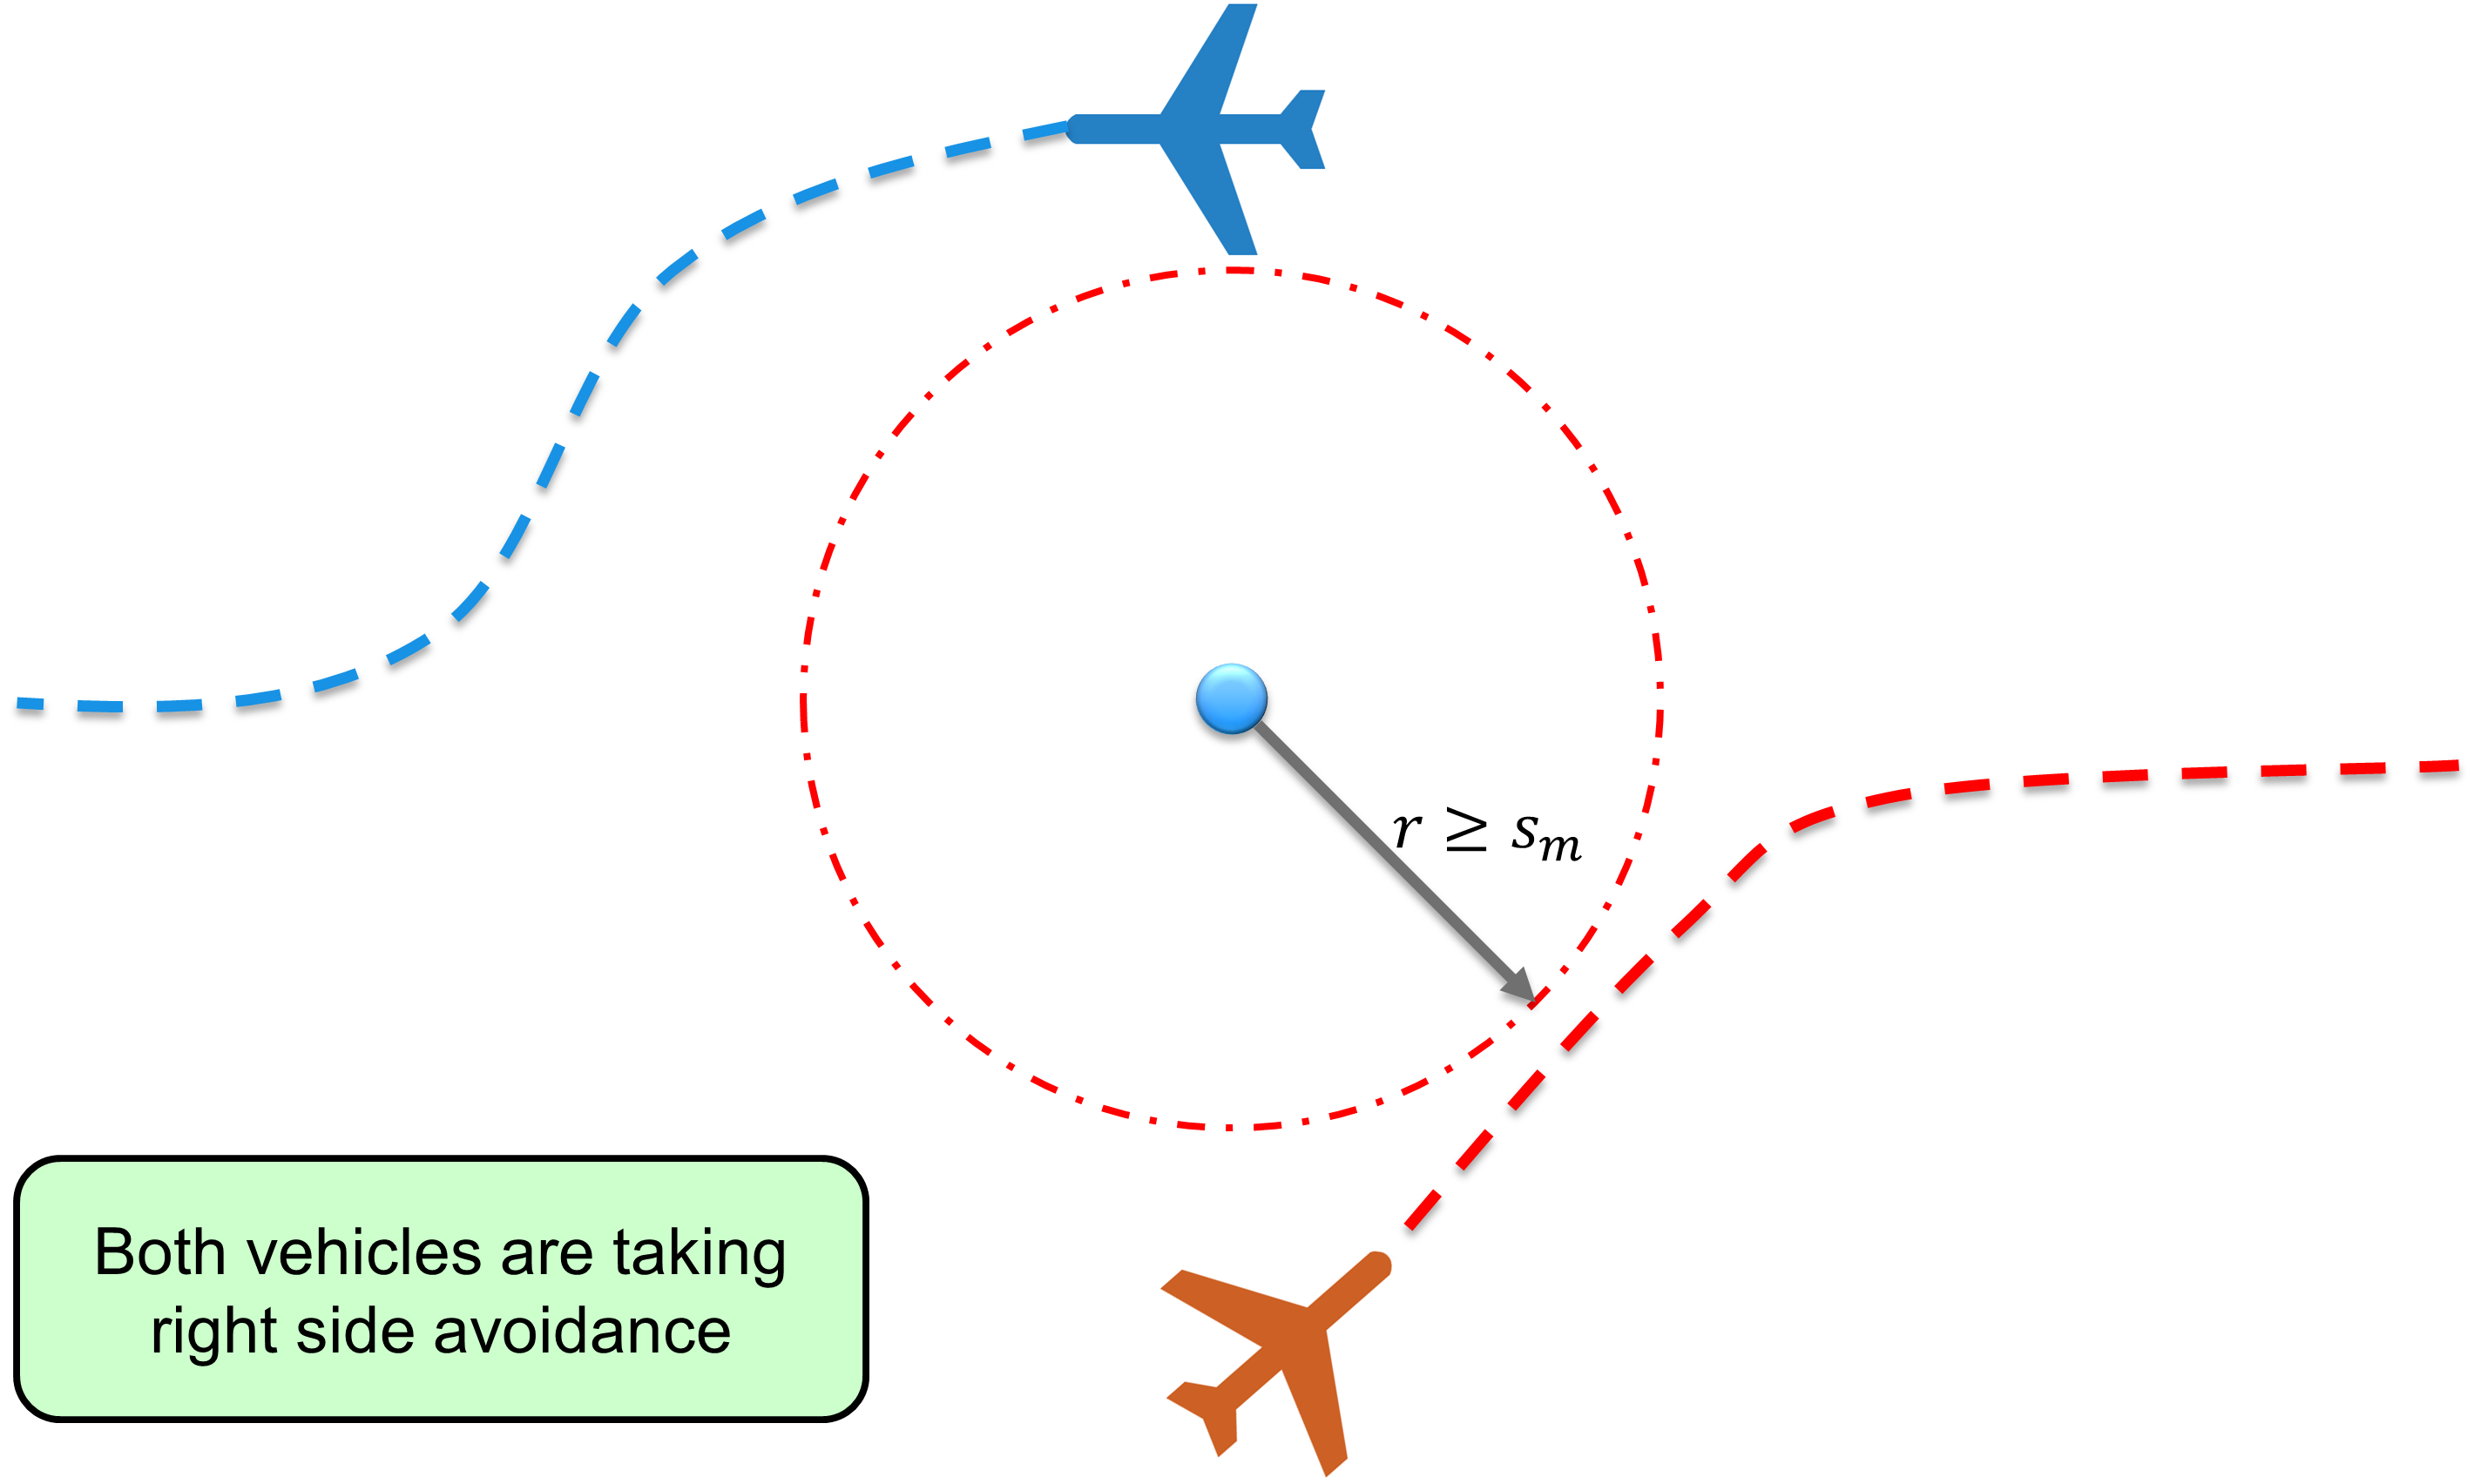
\includegraphics[width=0.9\linewidth,height=95pt,keepaspectratio]{\FIGDIR/RE009HeadOnApproach02} 
        \caption{Resolution/Closing.}
        \label{fig:HeadOnApproachTheoreticalResolution}
    \end{subfigure}
    \caption{Head-on approach detection/resolution/Closing}
    \label{fig:HeadOnApproachTheoretical}
\end{figure}

\paragraph{Triggering Events:} The \emph{head-on approach} (fig. \ref{fig:HeadOnApproachTheoretical}) \emph{triggering events} are the following:
\begin{enumerate}
    \item \emph{Detection} (fig. \ref{fig:HeadOnApproachTheoreticalDetection}) - the \emph{collision case} is open when \emph{collision point} with the respective angle of approach is detected. This must happen until the \emph{point of no return} is achieved. 
    
    \item \emph{Resolution} (fig. \ref{fig:HeadOnApproachTheoreticalResolution}) - the \emph{virtual} roundabout is enforced until the closing condition is met. 
    
    \item \emph{Closing} (fig. \ref{fig:HeadOnApproachTheoreticalResolution}) - based on the condition that all vehicles are heading away from \emph{collision point} and their mutual heading is neutral or opposite.
\end{enumerate} 

\paragraph{Virtual roundabout:} The \emph{flight levels} can be abstracted as the  \emph{virtual 2D surface}. The \emph{airspace attendants} are moving on virtual routes which can cross each other. The idea is to create virtual roundabout with enforced velocity to enable smooth collision avoidance.

\begin{enumerate}
    \item \emph{Center} - the center defined in \emph{airspace cluster} local coordinate system (flight level defining the horizontal placement).
    
    \item \emph{Diameter} - the minimal distance to \emph{center}, accounting the \emph{wake turbulence} and other phenomena. 
    
    \item \emph{Enforced velocity} - all attendants at \emph{virtual roundabout} keeps the same velocity. It helps to keep constant mutual distances.
\end{enumerate}



\subsection{Handling Converging Maneuver}\label{sec:handlingConvergingManuever}

\paragraph{Summary:} Two planned trajectories of the UAS are perpendicular, thus resulting in a protentional collision.  There is a need to define triggers for detection and resolution approach for autonomous UAS.  Rules for VFR/IFR modes in manned aviation are the base for the autonomous collision resolution.

\paragraph{Goal:} Identify \emph{required parameters} sufficient for automatic solution of \emph{Converging Maneuver}.

\paragraph{VFR:} The \emph{Visual Flight Rules} (VFR) are specified in annex 2 \cite{icaoAnnex2}. The rule is different from \emph{Head-on Approach} (sec. \ref{sec:handlingHeadOnApproach}) because multiple roles are depending on the relative aircraft position:
\begin{enumerate}
    \item \emph{Avoiding Aircraft} - there is an aircraft on the relative right side (blue). 
    \item \emph{Right Of the Way (ROA) Aircraft} - there is an aircraft on the relative left side (red). 
\end{enumerate}

The \emph{avoiding aircraft} should take the \emph{right of the way aircraft} from behind, with sufficient \emph{safety margin}, and return to original \emph{heading} afterward. The \emph{magnitude} of \emph{avoidance curve} must consider \emph{wake turbulence} and other impacts of \emph{avionic properties}.

\begin{note}
    This rule is applied only when both \emph{aircraft} belong to the same  \emph{maneuverability class} \cite{icaoAnnex2}.
\end{note}

\paragraph{IFR:} The \emph{Instrument Flight Rules} in annex 2. \cite{icaoAnnex2} and 11. \cite{icaoAnnex11} are defining \emph{converging maneuver} in detail.

The \emph{parameters} from a \emph{head-on approach} can be reused:
\begin{enumerate}
    \item $70^\circ$ $\le$ the \emph{Angle of Approach} $<$ $130^\circ$ - the minimal planar angle between aircraft position and expected collision point is in the interval $[70^\circ , 130^\circ[$.
    
    \item\emph{Minimal detection range} - given as $turning Radius + safety Margin$, while \emph{safety margin} is accounting all impact factors. 
    
    \item\emph{Safety margin} - during avoidance all aircraft keeps mutual distance at least on the value of \emph{Safety Margin}.
\end{enumerate}

\begin{note}
The lesser \emph{angle of approach} induces stronger wake turbulence impact on avoiding aircraft. This results in an increase of \emph{safety margin}. 

The \emph{wake turbulence} is represented as a droplet at the back of the plane. \emph{Wake turbulence range} can be calculated based on wake turbulence cone.
\end{note}

\begin{figure}[H]
	\centering
    \begin{subfigure}{0.32\textwidth}
    	\centering
        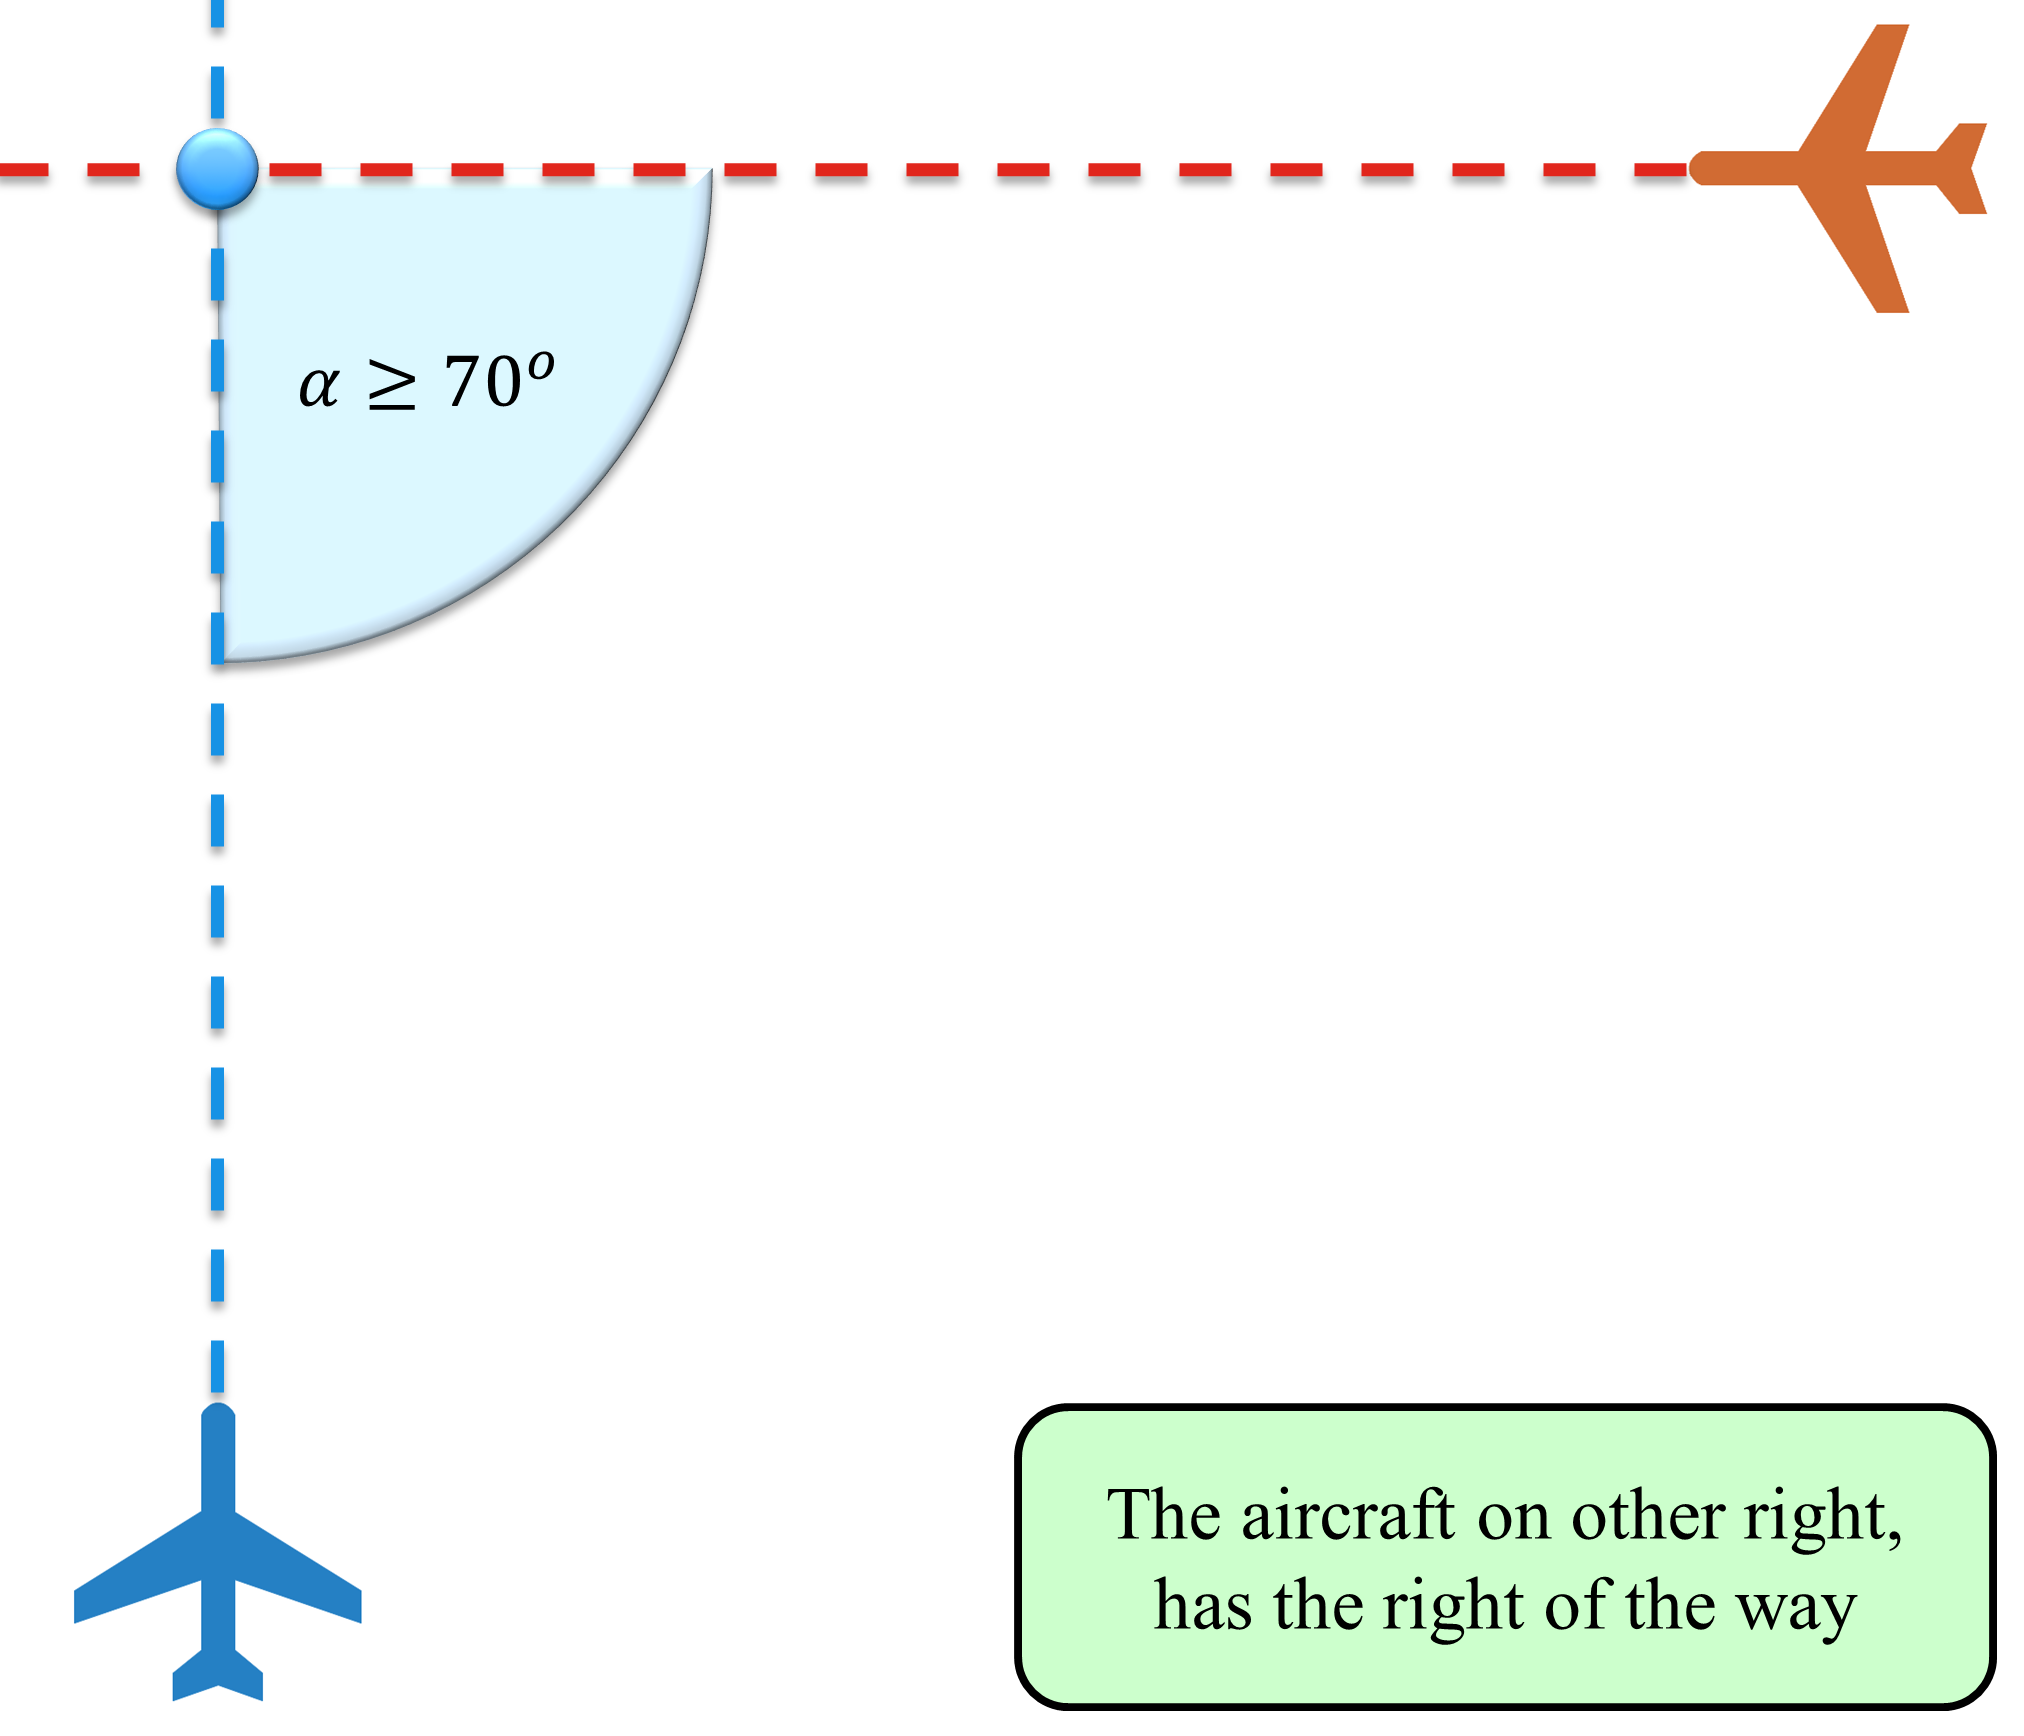
\includegraphics[width=0.9\linewidth,height=105pt,keepaspectratio]{\FIGDIR/RE005ConvergingManeuver01} 
        \caption{Detection.}
        \label{fig:ConvergingManeuverTheoreticalDetection}
    \end{subfigure}
    \begin{subfigure}{0.32\textwidth}
        \centering
        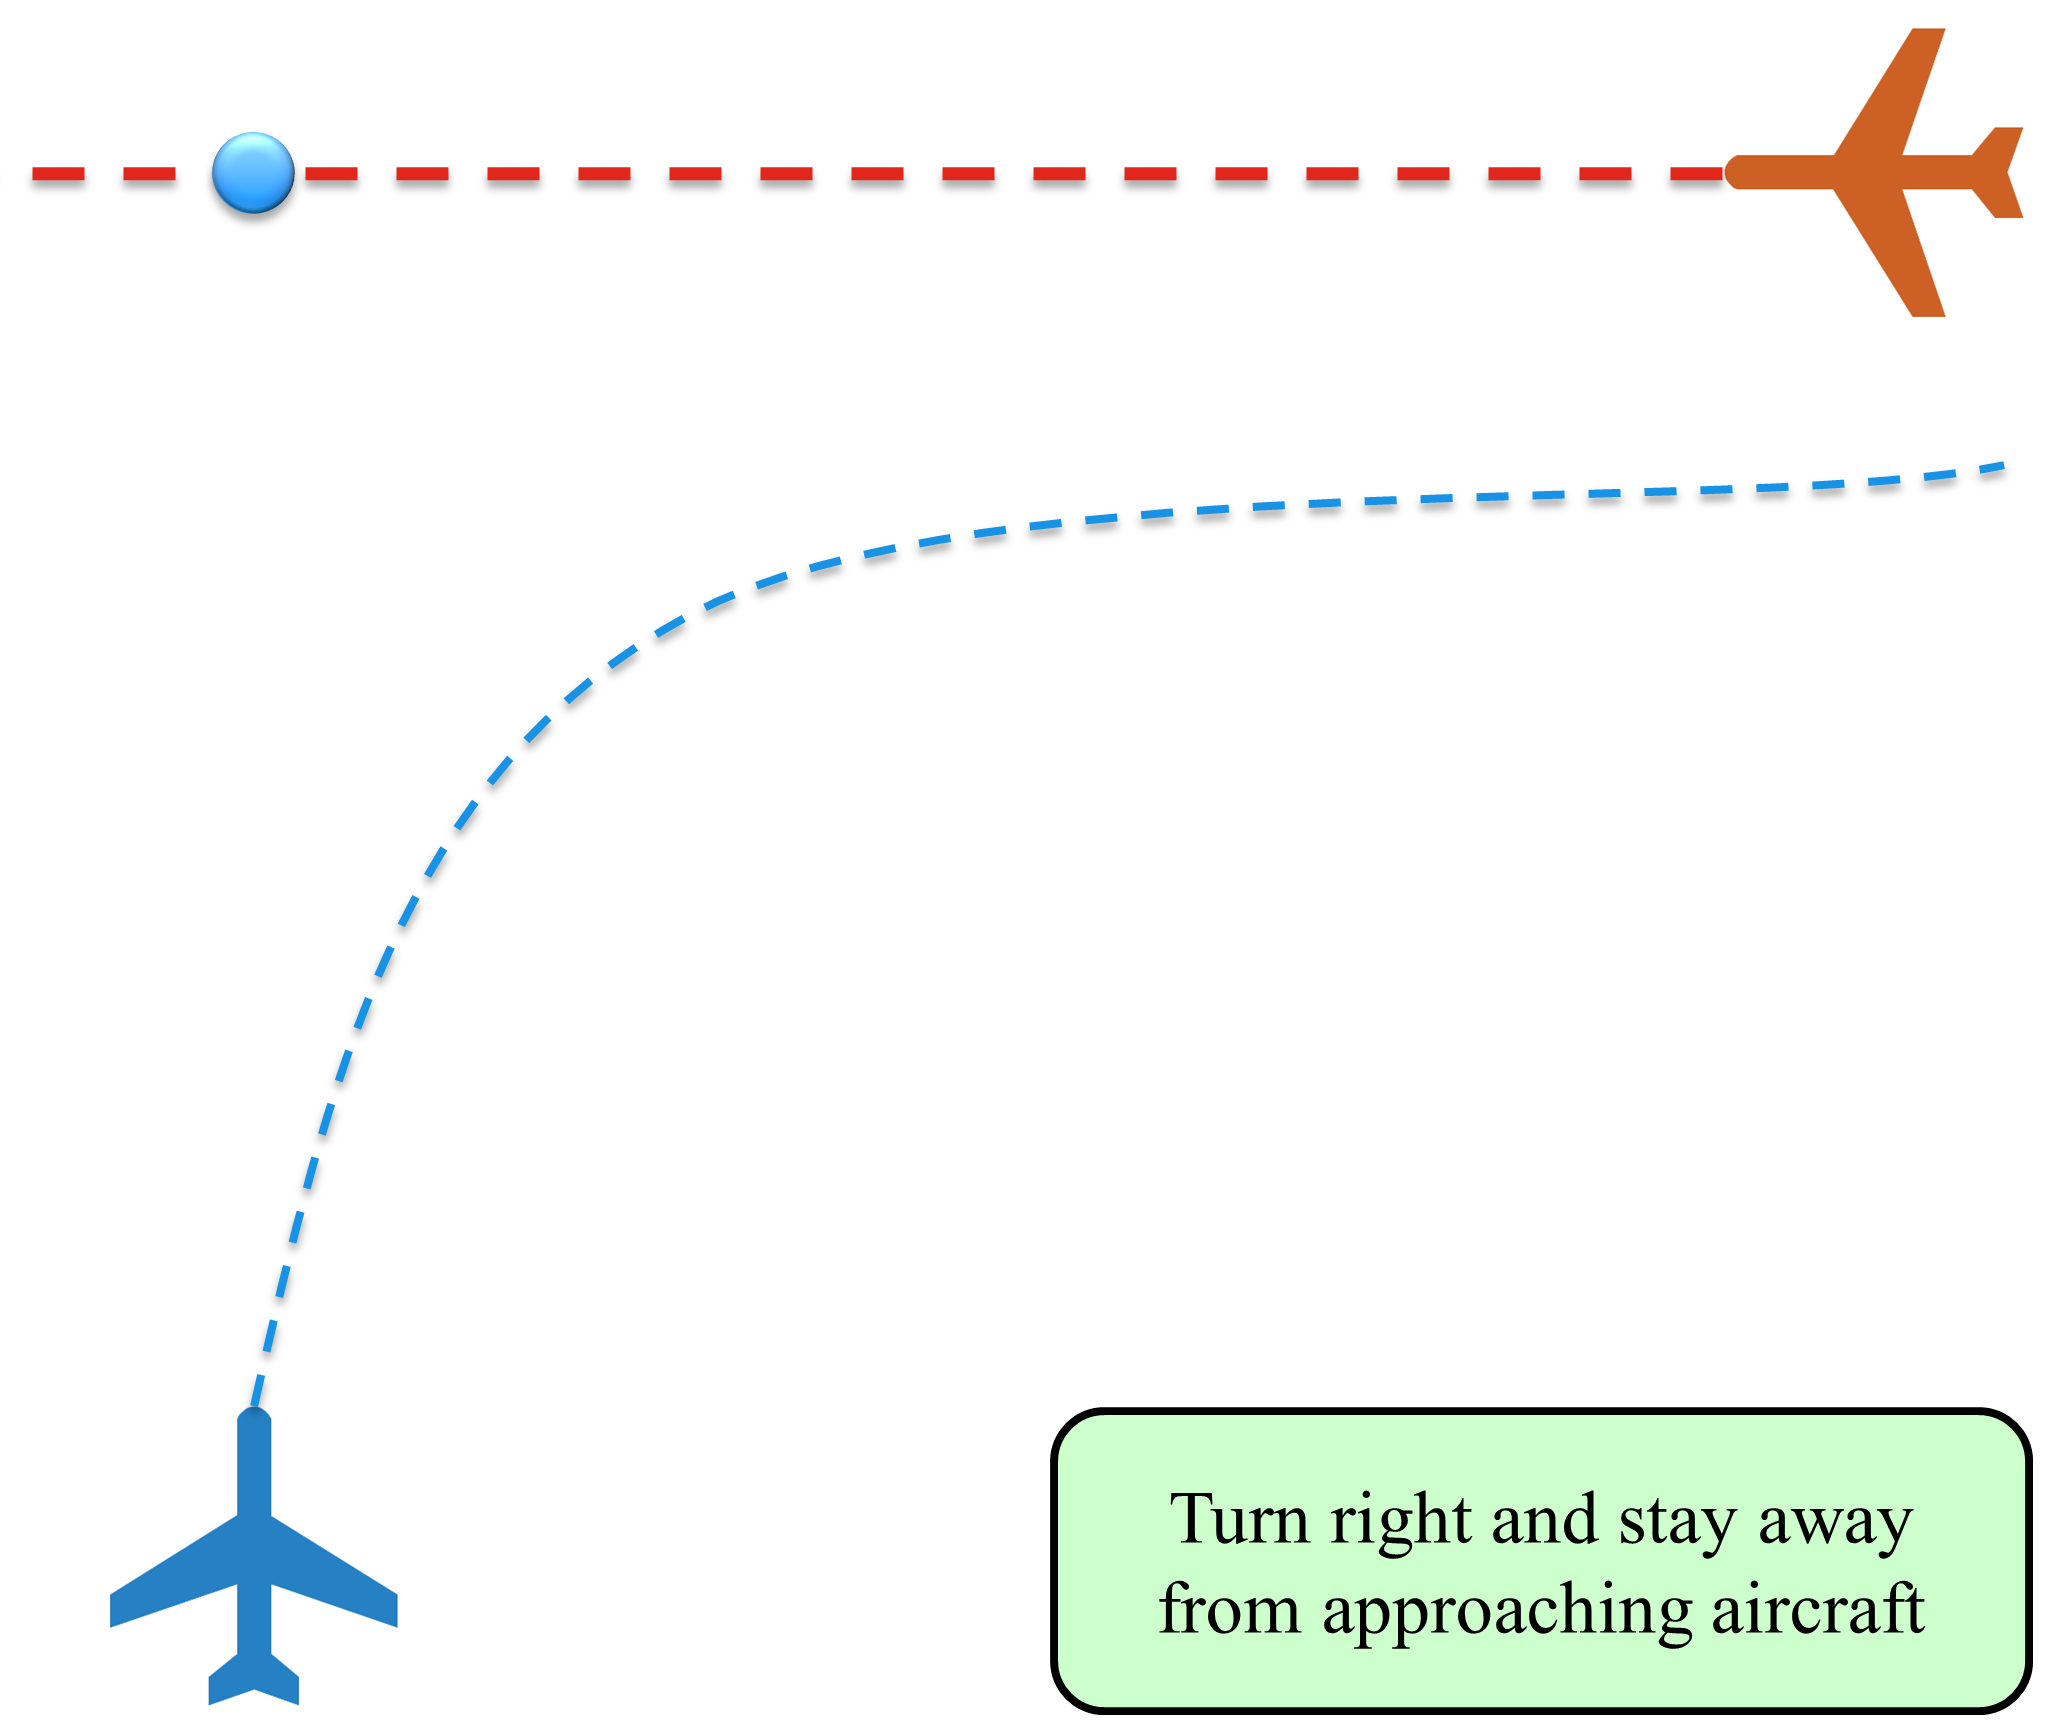
\includegraphics[width=0.9\linewidth,height=105pt,keepaspectratio]{\FIGDIR/RE006ConvergingManuever02} 
        \caption{Resolution.}
        \label{fig:ConvergingManeuverTheoreticalResolution}
    \end{subfigure}
    \begin{subfigure}{0.32\textwidth}
        \centering
        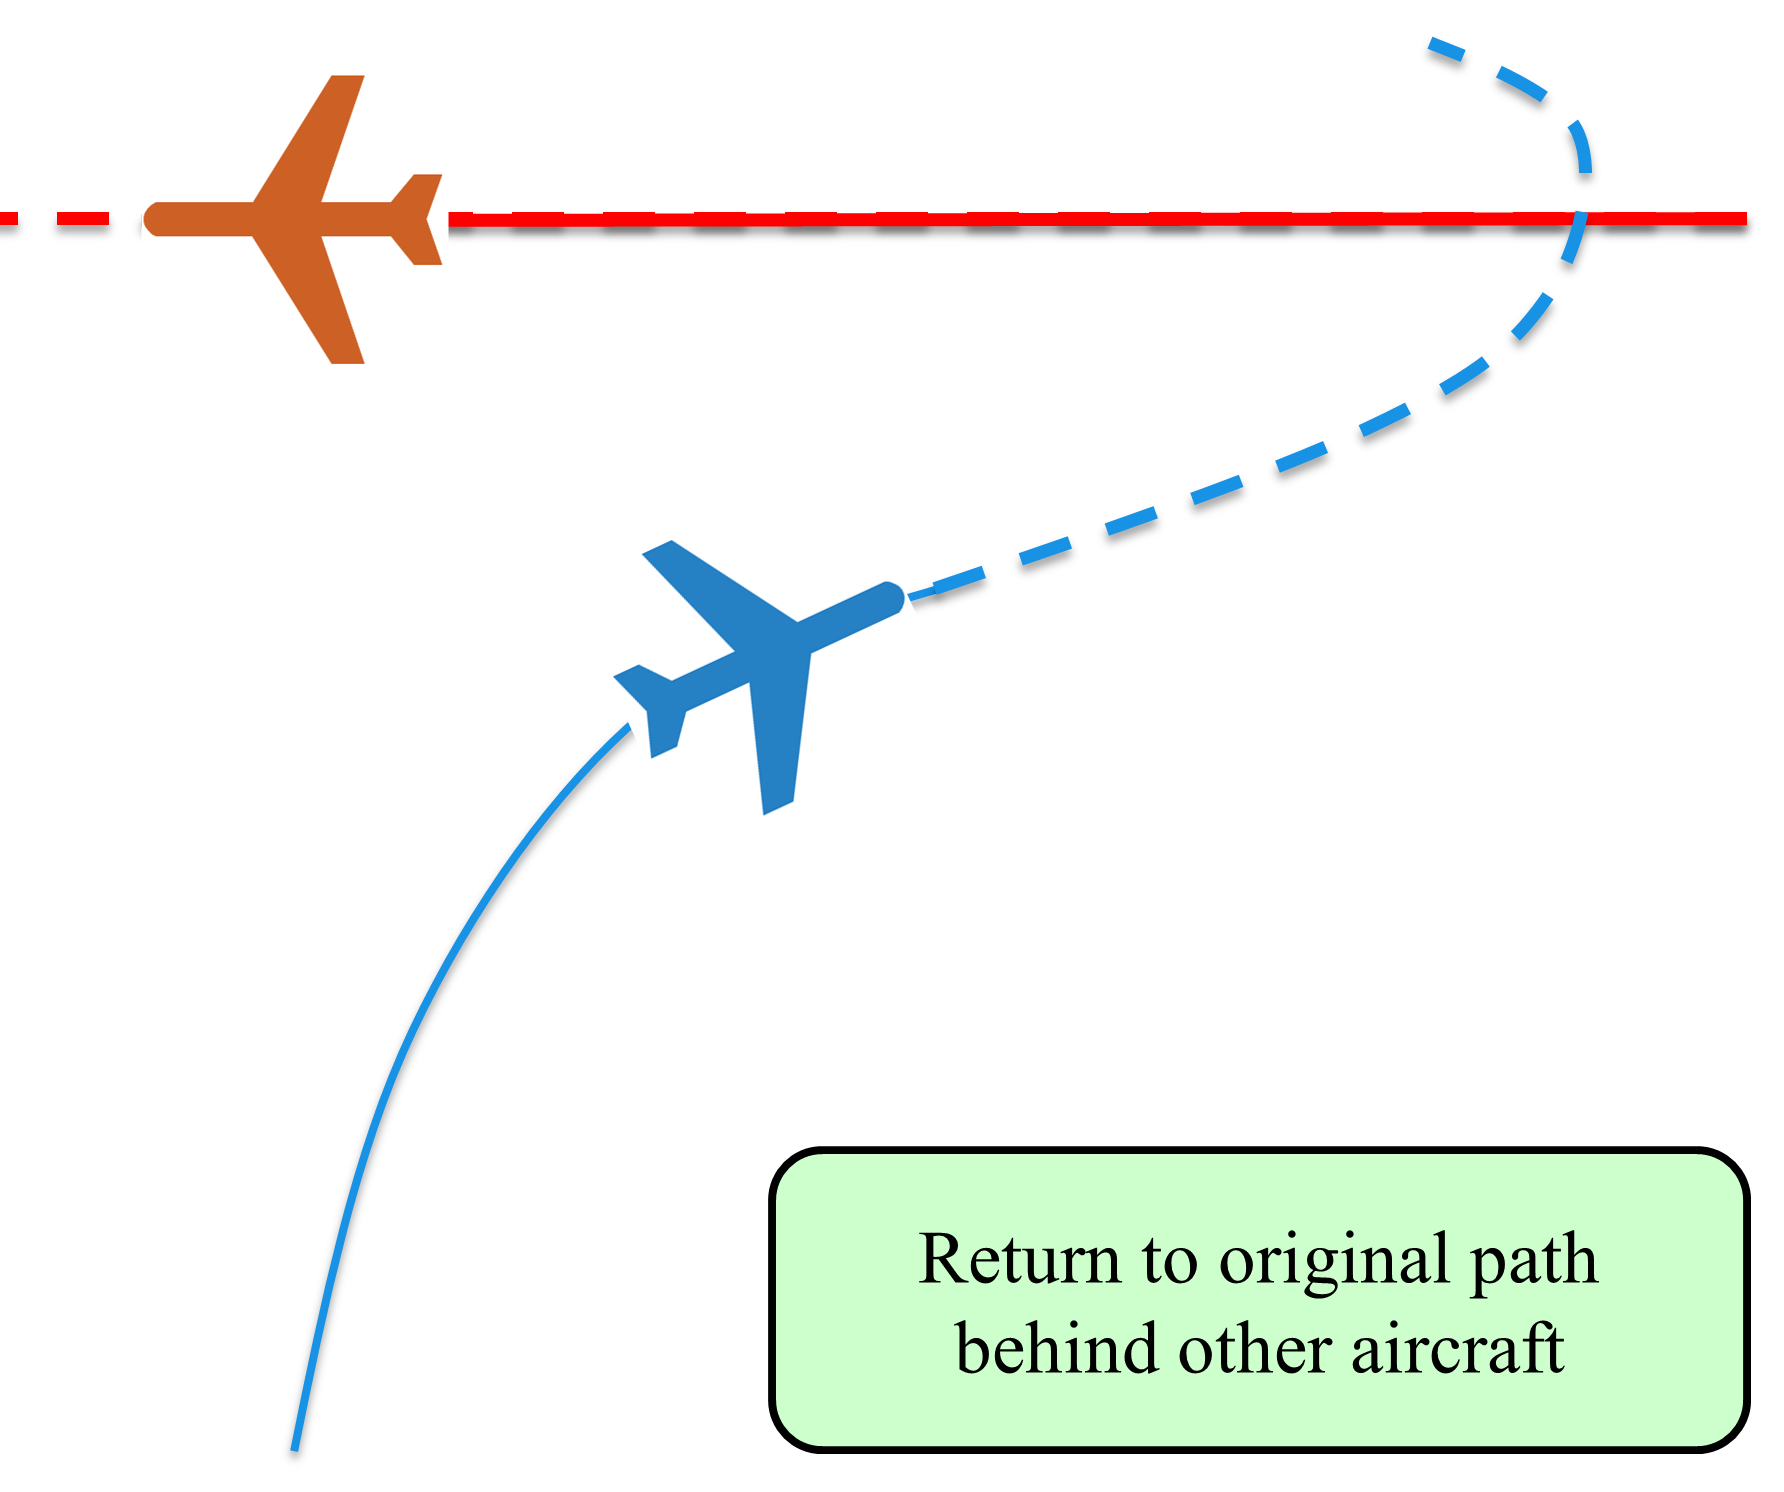
\includegraphics[width=0.9\linewidth,height=105pt,keepaspectratio]{\FIGDIR/RE007ConvergingManuever03} 
        \caption{Closing}
        \label{fig:ConvergingManeuverTheoreticalClosure}
    \end{subfigure}
    \caption{Converging maneuver Detection/Resolution/Closing}
    \label{fig:ConvergingManeuverTheoretical}
\end{figure}

\paragraph{Triggering Events:} The \emph{converging maneuver} (fig. \ref{fig:ConvergingManeuverTheoretical}) \emph{triggering events} are the following:

\begin{enumerate}
    \item \emph{Detection} (fig. \ref{fig:ConvergingManeuverTheoreticalDetection}) -  The \emph{avoiding airplane} (blue) detects \emph{collision point} (blue circle) which satisfy the \emph{converging maneuver conditions}. The distance between \emph{aircraft position} and \emph{collision point} is lesser than the \emph{detection range}.
    
    \item \emph{Resolution} (fig. \ref{fig:ConvergingManeuverTheoreticalResolution}) - the \emph{Right Of the Way aircraft} (red) stays at the original course. The \emph{avoiding aircraft} (blue) follows the \emph{parallel} to another \emph{plane}. The distance of \emph{avoiding plane} to \emph{other plane trajectory} is greater or equal to \emph{safety margin}.
    
    \item \emph{Closing} (fig. \ref{fig:ConvergingManeuverTheoreticalClosure}) - when both planes have an opposite heading, and they miss each other the converging maneuver can be closed. The \emph{avoiding airplane} will return to \emph{original trajectory}  while keeping the distance from \emph{another plane} (red) at greater or equal to \emph{safety margin}.
\end{enumerate}


\subsection{Handling Overtake Maneuver}\label{sec:handlingOvertakeManuever}

\paragraph{Summary:} Two UAS are on the same airway, flying in the same direction. The slower UAS is in front of the faster UAS. The slower UAS has the right of way, and the faster UAS needs to make an overtake. There is a need to define triggers for detection and resolution approach for autonomous UAS.  Rules for VFR/IFR modes in manned aviation are the base for the autonomous collision resolution.

\paragraph{Goal:} Identify \emph{required parameters} sufficient for automatic solution of \emph{Overtake Maneuver}

\paragraph{VFR:} The \emph{Visual Flight Rules} (VFR) are specified in annex 2 \cite{icaoAnnex2}. The rule states that faster air traffic attendant may overtake slower one, from right side keeping sufficient distance (\emph{safety margin}). There are two forced roles:

\begin{enumerate}
    \item \emph{Overtaking} - faster aircraft with similar heading cruising in similar altitude than \emph{overtaken} (blue). It is expected that \emph{faster aircraft} has maneuvering capability to avoid slower aircraft.
    
    \item \emph{Overtaken} - slower aircraft which keeps the \emph{Right of the way}
\end{enumerate}

\begin{note}
    This rule is applied only when both aircraft have the same maneuverability class \cite{icaoAnnex2}. The overtake is considered \emph{borderline emergency maneuver} in controlled airspace because the aircraft tend to keep similar velocity in similar cruising altitude. The overtake is usual in \emph{non-controlled airspace}.
\end{note}

\begin{figure}[H]
	\centering
    \begin{subfigure}{0.32\textwidth}
        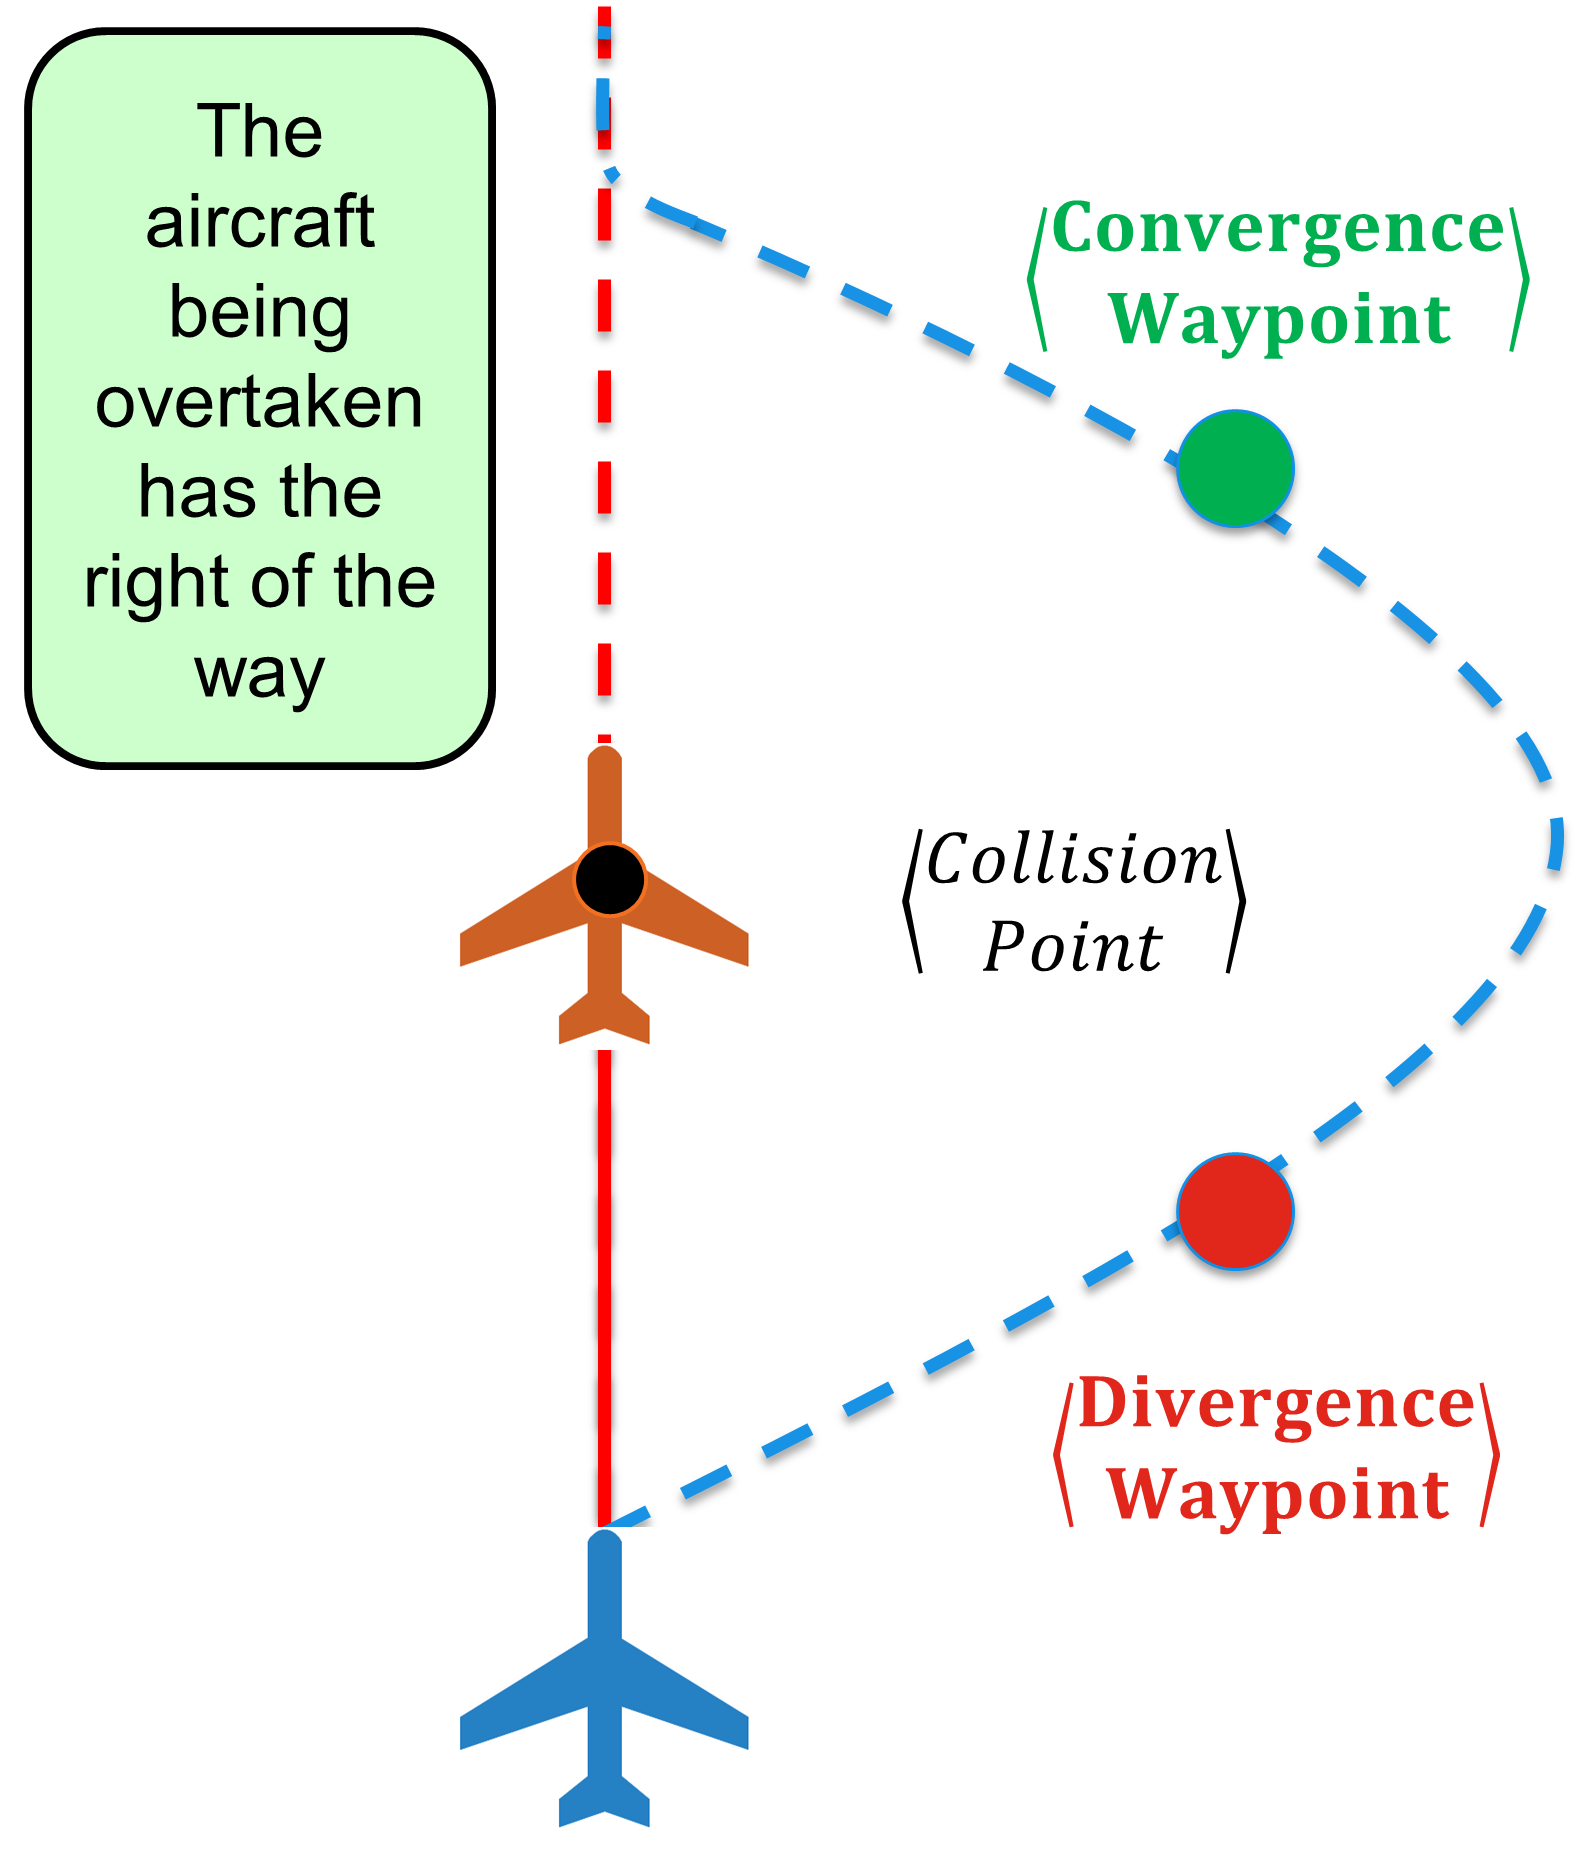
\includegraphics[width=0.9\linewidth,height=142pt,keepaspectratio]{\FIGDIR/RE010OvertakeMAnuever01} 
        \caption{Detection.}
        \label{fig:OvertakeManeuverTheoreticalDetection}
    \end{subfigure}
    \begin{subfigure}{0.32\textwidth}
        \includegraphics[width=0.9\linewidth,height=142pt,keepaspectratio]{\FIGDIR/RE011OvertakeMAnuever02} 
        \caption{Resolution.}
        \label{fig:OvertakeManeuverTheoreticalResolution}
    \end{subfigure}
    \begin{subfigure}{0.32\textwidth}
        \includegraphics[width=0.9\linewidth,height=142pt,keepaspectratio]{\FIGDIR/RE012OvertakeMAnuever03} 
        \caption{Closing.}
        \label{fig:OvertakeManeuverTheoreticalClosure}
    \end{subfigure}
    \caption{Overtake maneuver Detection/Resolution/Closing}
    \label{fig:OvertakeManeuverTheoretical}
\end{figure}

\paragraph{IFR:} The \emph{Instrument Fight Rules} in annex 2. \cite{icaoAnnex2} and 11. \cite{icaoAnnex11} are defining the converging manual in detail:

\begin{enumerate}
    \item 0$^\circ \le$ the \emph{Angle of Approach} $<$ 130$^\circ$ - the minimal planar angle between aircraft position and expected collision point is in the interval $[0^\circ,70^\circ[$
    
    \item \emph{Minimal Detection Range} - given as $2 \times  reaction Time \times speed Difference$. 
    
    \item \emph{Safety Margin} - during avoidance the overtaking aircraft keeps the minimal distance of \emph{wake turbulence} of overtaken aircraft in own flight altitude. 
\end{enumerate}

\begin{note}
    The \emph{Safety Margin} is sufficiently small because speed difference is usually much lesser than in case of  \emph{Head-on approach}. The \emph{Wake turbulence} can be avoided completely by taking the higher altitude level than overtaken aircraft.
\end{note}


\paragraph{Triggering events:}
\begin{enumerate}
    \item \emph{Detection} (fig. \ref{fig:OvertakeManeuverTheoreticalDetection}) - occurs when the distance between \emph{overtaking} (blue) and overtaken (red) is approaching \emph{minimal detection range} or double of \emph{safety margin}. If the performance of \emph{overtaking aircraft} (blue) allows taking \emph{sharp right side to overtake} the \emph{Maneuver starts}, otherwise \emph{overtaking aircraft} (blue slows down) and keeps at least \emph{safety margin distance} to avoid \emph{wake turbulence}.
    
    \item \emph{Resolution} (fig. \ref{fig:OvertakeManeuverTheoreticalResolution}) - \emph{overtaken} (red) is keeping same heading and \emph{speed} during overtake maneuver. The \emph{overtaking} (blue) projects two waypoints: \emph{Divergence} and \emph{Convergence} keeping the required separation minimum during overtake. Then the \emph{overtaking} (blue) diverges heading to \emph{Divergence waypoint}. When the \emph{Divergence waypoint} is reached by \emph{overtaking} (blue) aircraft, it changes to \emph{original heading}.
    
    \item \emph{Closing} (fig. \ref{fig:OvertakeManeuverTheoreticalClosure}) - the \emph{closing} of \emph{Overtake} starts when \emph{overtaking} aircraft (blue) have sufficient lead over \emph{overtaken} aircraft (red). The \emph{overtaking} aircraft (blue) can safely change the heading to the original waypoint.
\end{enumerate}


\paragraph{Constant Cruising Speed:} Most of the traffic attendants at same flight level have similar (close to constant) cruising speed. Lower flight levels are for slower turbo-prop planes, and higher altitudes are for jet planes. It is stated that this principle will persist even when UAS will be integrated \cite{bayen2005langrangian,kopardekar2002dynamic,helme1992optimization} in multiple air-traffic models.



		\subsection{\secState{R}Position Notification}\label{sec:positionNotification}

\paragraph{Motivation:} The \emph{position notification} (tab. \ref{tab:positionNotification}) is designed for further \emph{collision case resolution} (sec. \ref{sec:collisionCase}). It is similar to ADS-B\footnote{ADS-B versions and message containment: \url{https://mode-s.org/decode/adsb/version.html}.} message information. 


The main purpose is to broadcast the \emph{position notification} in \emph{controlled aerospace}. The broadcast for \emph{non-controlled} airspace needs to contain \emph{intruder properties}, \emph{preferred separation mode} and \emph{near-miss margin}.

\paragraph{Position:} The position is defined in \emph{Global Coordinate System} using GPS for latitude and longitude. The barometric altitude is required for controlled airspace, preferred for non-controlled airspace.

\paragraph{Heading:} The \emph{Linear Velocity} combined with heading in standard \emph{North-East} coordinate frame is used.

\paragraph{Flight Levels:} The \emph{flight level} is notified to UTM for \emph{collision detection} purposes. There is a \emph{main flight level} where \emph{aircraft} belong physically. There is a \emph{passing flight level} form which/to which is aircraft emerging \cite{icao4444}. 

\paragraph{Aircraft Category:} The aircraft category impacts the prioritization of \emph{role assessment} by UTM/ATM. The following categorization is proposed by \emph{manned aviation pilot community}, from the highest to the lowest right of the way priority:

\begin{enumerate}
    \item \emph{Manned aviation in distress} \cite{icaoAnnex2} -  the aircraft with impaired capability switched to emergency mode. The emergency mode is usually acknowledged by the authority in controlled airspace. 
    
    \item \emph{Balloon} (manned) \cite{icaoAnnex2} - the aircraft with \emph{altitude} control and very slow dynamics implying very low maneuverability.  
    
    \item \emph{Glider} (manned) \cite{icaoAnnex2} - the aircraft with \emph{full control} but without own \emph{propulsion}. The overall \emph{maneuverability} is good, but the \emph{velocity} changes are impossible with sufficient flexibility.
    
    \item \emph{Aerial towing} (manned) \cite{icaoAnnex2} - the towing aircraft usually have \emph{own propulsion} and full maneuverability, the only constraint is \emph{towed load}. The towed load decreases overall maneuverability.
    
    \item \emph{Airship} (manned) \cite{icaoAnnex2} - the airship have \emph{own propulsion} and full maneuverability, the constraint is low acceleration/deceleration and huge turning radius.
    
    \item \emph{Other manned aviation} \cite{icaoAnnex2} - containing all vehicles with the required level of \emph{airworthiness} for given operational \emph{altitude}. They usually have required maneuverability.
    
    \item \emph{UAS Autonomous} (proposed) \cite{santiago2015pilot} - containing all autonomous UAS, the lower flexibility is expected at the beginning of integration.
    
    \item \emph{Remotely Piloted Aerial System (RPAS)} (proposed)  \cite{santiago2015pilot} - has lesser priority due to the higher response rate of the pilot.
\end{enumerate}

\begin{note}
    This categorization reflects only Pilot community statement; the general priority rule is broken, because maneuverability and vulnerability  should always be considered as a key decision factor. 
\end{note}


\paragraph{Maneuverability:} The maneuverability is the real key factor in priority assessment.  The components of maneuverability are \emph{maximal/mean acceleration/deceleration}, \emph{climb/ descent rate} and \emph{turning ratio/radius}. The comparison can be made by solving \emph{pursuit problem} using \emph{Reach Sets} \cite{game1987,game1988}.

\noindent The \emph{Maneuverability categorization} is based on \emph{original aircraft priority categorization} \cite{icaoAnnex2} accounting UAS/RPAS as equal to \emph{manned aviation}. The ordered list from the highest to the lowest priority goes as follows:

\begin{enumerate}
    \item \emph{Impaired control} (Distress aircraft) - any aviation attendant in distress has the priority in case of the conflict occurrence.
    
    \item \emph{Altitude control/No} (Balloon, Hovering aircraft) - the balloon type crafts do not have any type of propulsion, and horizontal movements follow the airflow in given altitude. 
    
    
    \item \emph{Full control/No propulsion} (Gliders of any sort) - the gliders can control their horizontal position, but there are limits to altitude control and acceleration/deceleration. 
    
    \item \emph{Full control/Linear propulsion} (Any aircraft of plane type) - the \emph{towing aircraft's} and \emph{airplanes} belong there; the difference is the \emph{flexibility} of \emph{maneuvering}.
    
    \item \emph{Full control/VTOL capability} (Any aircraft with VTOL) - the \emph{other aircraft} capable of doing on-spot-turn. The typical representative is \emph{quad-rotor copter}.
\end{enumerate}



\begin{tabularx}{\textwidth}{S{0.25}|X}
     \multicolumn{2}{c}{\textbf{Position}}  \\\hline
     latitude & based on GPS/IMU sensor fusion.\\
     longitude & based on GPS/IMU sensor fusion.\\
     altitude & barometric altitude \emph{Above Mean Sea Level} (AMSL). \\         
     \multicolumn{2}{c}{\textbf{Heading}}  \\\hline
     orientation & orientation in standard North-East coordinate frame.\\
     velocity & relative UAS velocity.\\
     \multicolumn{2}{c}{\textbf{Flight Levels}}\\\hline
     main & flight level, where UAS mass center belongs\\
     passing & flight level, during climb/ascend, or when distance of UAS mass center to flight level boundary $\le 250 ft$ .\\
     \multicolumn{2}{c}{\textbf{Registration}}\\\hline
     registration ID& is unique registration number \emph{to be issued} by local aviation authority for UTM communications purposes.\\
     flight code& or mission code is a unique identification number for approved mission plan which is going to be flown by UAS.\\
     UAS name & optional UAS identifier to increase human recognition. \\
     \multicolumn{2}{c}{\textbf{Categorization}}\\\hline
     craft category & ICAO main category, based on vehicle type.\\
     maneuverability& secondary categorization is specifying size class, horizontal/vertical turning radius, minimal and maximal cruising speed.\\
     \multicolumn{2}{c}{\textbf{Safety margins}}\\\hline
     universal & minimal safety margin for any avoidance situation\\
     head-on & minimal distance from other similar maneuverability class aircraft in case of a head-on approach.\\
     converging & minimal distance from other similar maneuverability class aircraft in case of the converging maneuver.\\
     overtake & minimal distance from other similar maneuverability class aircraft in case of overtake maneuver.\\
     wake angle & for wake turbulence cone.\\
     wake radius & for wake turbulence cone.\\
    \caption{Time-stamped \emph{position notification} structure.}
    \label{tab:positionNotification}
\end{tabularx}

There are other aspects like \emph{minimal required} acceleration/deceleration/turn ratio to operate in a selected segment of the \emph{airspace}. These should be specified later by \emph{Minimum Operational Performance Standards} (MOPS).

\paragraph{Safety Margins:} The \emph{Safety Margin} for \emph{Well Clear Condition} value is based on the \emph{situation}. There is also a \emph{universal safety margin} which guarantees the minimal safety for encountering intruder. 

The most prevalent effect is \emph{Wake turbulence}, therefore, \emph{wake turbulence cone} angle $[0\circ -90\circ ]$ and radius. 

The \emph{safety Margin} for situation-based avoidance is given by the list of supported  maneuvers; there is converging (sec. \ref{sec:handlingConvergingManuever}), head-on (sec. \ref{sec:handlingHeadOnApproach}), overtake (sec. \ref{sec:handlingOvertakeManuever}) safety margins.



		\subsection{\secState{R}Collision Case}\label{sec:collisionCase}


\paragraph{Collision Case Purpose:} There is a need for detection and tracking of possible \emph{controlled airspace traffic attendants} collisions.  The presented \emph{collision case structure} (tab. \ref{tab:collisionCase}) is minimalist reflection of \emph{ATM} requirements. Following aspects of  \emph{collision case} life cycle are explained in this section:
\begin{enumerate}
    \item \emph{Base terminology} - the definition of \emph{enforcement procedure} and difference between \emph{Resolution} and \emph{Mandate} from UTM authority. The \emph{severity issue} is open.
    
    \item \emph{Calculation of single case for single decision frame} - step by step calculation and threat evaluation. Prequel to \emph{life cycle}.
    
    \item \emph{Life cycle} gives outlook how collision case data are handled trough longer period of time, notably: \emph{Opening}, \emph{collision point handling}, \emph{safety margin handling}, and, \emph{Closure}.
    
    \item \emph{Merge procedure for multiple cases in single cluster} - the naive \emph{merge procedure} to solve \emph{multiple collision cases} via \emph{virtual roundabout}.
\end{enumerate}


\paragraph{Resolution/Mandate Enforcement:}
\emph{Enforcement procedure} is consisting from \emph{Threat detection phase} and \emph{Mitigation phase}. The \emph{mitigation phase} is a time interval when \emph{UTM} decision is enforced. The decision the UTM is enforcing is delivered in form of \emph{Resolutions} and \emph{Mandates}.


\emph{Resolution} is an order from the \emph{UTM} authority which is followed by subjected UAS. The \emph{subjected UAS} can determine own behaviour to some extent. When there is emerging threat or other destructive event, like new non-cooperative adversary, the UAS is allowed to broke \emph{resolution}.  

\emph{Mandate} is an order from the \emph{UTM} authority which can not be broken at any cost. The example of the \emph{mandate}: UAS is flying in airspace, the passenger in distress needs it to safely land. The UAS must obey mandate even at event of own destruction.

\paragraph{Threat Severity Evaluation:} The threat severity evaluation is omitted partialy, all threats are considered as equal. All commands from \emph{UTM authority} will be considered as \emph{resolutions}.

\paragraph{Calculation procedure:} Collision case is calculated for two \emph{Registered UAS systems} in \emph{Unified UTM time-frame}. The \emph{unified UTM time-frame} is a short period of time in future when the anticipated situations are predicted. 

\paragraph{1\textsuperscript{st}} The \emph{position} and \emph{orientation} is adjusted according to \emph{mission plan}. Our implementation uses \emph{Movement Automaton} as a predictor:
\begin{equation}
\begin{gathered}
    adjustedPosition = Position(Trajectory(notifiedState, futureMovements))\\
    adjustedOrientation = Orientation(Trajectory(notifiedState, futureMovements))
\end{gathered}
\end{equation}

\noindent For other cases standard linear prediction can be used:
\begin{equation}
    \begin{gathered}
        adjustedPosition = notificationPosition \times notificationVelocity \times timeDifference\\
        adjustedOrientation = notificationOrientation
    \end{gathered}
\end{equation}

\paragraph{2\textsuperscript{nd}} The \emph{maneuverability}, \emph{craft category}, \emph{registration ID} are taken from \emph{position notification}.

\paragraph{3\textsuperscript{rd}} \emph{Collision case check procedure} goes like follows:
\begin{enumerate}
    \item \emph{Operation space checks} - the controlled airspace and flight level must match for proceeding.
    
    \item \emph{Maneuverability/Category check} - the maneuverability and UAS category must match. If there is mismatch then right of the way is forced to vehicle with higher priority.
\end{enumerate}

\paragraph{4\textsuperscript{th}} \emph{Linear Intersection test} is designed to calculate \emph{closest distance} and \emph{time} of \emph{linear trajectory projections},  First for given \emph{velocity} and \emph{position} for UAS1 and UAS2 the helper variables are calculated:
\begin{equation}
    \begin{aligned}
        A&=\norm{velocity_1}^2\\
        B&=2*({velocity_1}^T\times position_1-{velocity_2}^T\times position2)\\
        C&=2\times {velocity_1}^T *velocity_2\\
        D&=2*({velocity_2}^T \times position_2 - {velocity_2}' \times {position_1});\\
        E&=\norm{velocity_2}^2;\\
        F&=\norm{position_1}^2 + \norm{position_2}^2;\\
    \end{aligned}\\
\end{equation}
\noindent Then the projection parameters can be calculated:
\begin{equation}
    \begin{aligned}
    time& = \frac{-B-D}{2 \times A- 2 \times C+ 2 \times E}\\
    destination_i &= position_i + velocity_i \times time, \quad i \in \{1,2\}\\
    collisionPoint &= \frac{destination_1 + destination_2}{2}\\
    collisionDistance &= \norm{destination_1 - destination_2}\\
    \end{aligned}
\end{equation}

\noindent If $time < 0$ the trajectories are diverging from each other (because the closest points already occurred). The procedure ends, \emph{collision flag} is not raised.

If $time > time Margin$ the trajectories will get close to each other, but in further future and changes are anticipated. The procedure ends, \emph{collision flag} is not raised.

If $0 \le time \le timeMargin$ the trajectories are converging to each other and distance needs to be checked. If $distance \le collisionMargin$ then \emph{collision flag} is raised and \emph{collision point} is set.

\begin{note}
    \emph{Collision Margin} is some number which is determined based on aircraft category and maneuverability. Our work defines collision margin as follow:
    \begin{equation}
        collisionMargin = \forall situation : \max\left\{\begin{gathered}safetyMargin(situation,UAS1)\\ +safetyMargin(situation,UAS2) \end{gathered}\right\}
    \end{equation}
    
    Where \emph{safety margin} for every possible situation is evaluated for both \emph{UAS}.
\end{note}

\paragraph{5\textsuperscript{th}} The \emph{trajectory} intersection is \emph{Movement Automaton} specific collision detection method. Its based on the assumption that \emph{UTM} have following information from \emph{mission plan}:
\begin{enumerate}
    \item \emph{UAS state} - not only \emph{position}, \emph{orientation}, and, \emph{velocity} vectors, but other mathematical model parameters mandatory for \emph{movement automaton}.
    
    \item \emph{Movement Automaton} - movement automaton for our UAS system, so UTM can use it in predictor mode.
    
    \item \emph{Future Movements set} - up to reasonable prediction horizon $timeMargin$. 
\end{enumerate}

The \emph{Movement Automaton} can be used as trajectory prediction for system initial state and future movements.  The prediction function (eq. \ref{eq:statePredictionCollisionCase}).
\begin{equation}\label{eq:statePredictionCollisionCase}
    Prediction: UAS \times state \times future Movements \to [x,y,z,t] \in \R^4
\end{equation}

\begin{note}
    Then prediction for UAS1 is $Prediction_1$ and for UAS 2 $Prediction_2$, the predictions are synchronized meaning that time at position $i$ is equal in both discrete trajectory matrices.
\end{note}

The \emph{collision distance} for predictor (eq. \ref{eq:statePredictionCollisionCase}) is given as minimal distance of projected synchronized trajectories for UAS1 and UAS2. In our discrete enviroment the \emph{collision distance} is given as (eq. \ref{eq:TrajectoryPredictionMinimalDistance}).

\begin{equation}\label{eq:TrajectoryPredictionMinimalDistance}
    collisionDistance = \min\left\{\norm{point_1-point_2}:\forall \left(\begin{gathered}point_1 \in Prediction_1,\\ point_2, \in Prediction_2,\\ t_1 \sim t_2 \end{gathered}\right)\right\} 
\end{equation}

If $collisionDistance \le collision Margin$  condition is met, \emph{collision flag} is set.  

The collision point is then calculated  as mean of \emph{UAS positions} in prediction at time when distance is minimal.  The final collision point is arithmetic mean of two positions (eq. \ref{eq:collisionPointTrajectoryPrediction}).
\begin{equation}\label{eq:collisionPointTrajectoryPrediction}
    collisionPoint= \frac{point_1 - point_2}{2}:\left(\begin{gathered}point_1 \in Prediction_1,\\ point_2, \in Prediction_2,\\ t_1 \sim t_2 \text{ at minimal distance}\end{gathered}\right)
\end{equation}

\begin{note}
    Collision point is overwritten by trajectory intersection (specific) method, the \emph{linear intersection} is considered \emph{general collision detection method}. The collision detection method in future UTM system needs to be determined. The \emph{Trajectory intersection} method presented in this work is one of the possible candidates. 
\end{note}

\paragraph{6\textsuperscript{th}} \emph{Role determination} phase is invoked if and only if previous conditions are met and \emph{collision flag} with \emph{collision point} exists.

There is \emph{adjusted position} of each UAS used as verticals and \emph{collision point} used as center. First step is normalization of adjusted position around collision point for both UAS:
\begin{equation}
    normalized_i =  adjustedPosition_i - collisionPoint,\quad i \in \{1, 2\}
\end{equation}

Then the right hand coordinate system internal angle calculation method is used:


\begin{equation}
    angleOfApproach = \left|\text{atan2}\left(\begin{gathered}normalized_1 \times normalized_2, \\normalized_1 \circ normalized_2\end{gathered}\right)\right|
\end{equation}

\noindent Based on \emph{angle of approach} the \emph{scenario type} is  decided like follows:
\begin{enumerate}
    \item $130^\circ \le angle Of Approach  \le 180^\circ$ - the scenario type is set as \emph{Head On Approach} (sec.\ref{sec:handlingHeadOnApproach})
    \item $70^\circ \le angle Of Approach  < 130^\circ$ - the scenario type is set as \emph{Converging Maneuver} (sec.\ref{sec:handlingConvergingManuever})
    \item $0^\circ \le angle Of Approach  < 70^\circ$ and \emph{different speed} -   - the scenario type is set as \emph{Overtake Maneuver} (sec.\ref{sec:handlingOvertakeManuever})
\end{enumerate}

\noindent Based on \emph{relative position} and \emph{scenario type}, the \emph{avoidance role} like follows:
\begin{enumerate}
    \item \emph{Head On Approach} enforces following:
    \begin{enumerate}[a.]
        \item The \emph{avoidance role} us set as \emph{RoundAbounting} for both UAS.
        
        \item None of the \emph{UAS} does not have the \emph{Right Of the Way}.
    \end{enumerate}
    
    \item \emph{Converging Maneuver} enforces following:
    \begin{enumerate}[a.]
        \item \emph{UAS} without free right side have role set as \emph{Converging}.
        
        \item \emph{UAS} with free right side have the \emph{Right Of the Way}.
    \end{enumerate}
    
    \item \emph{Overtake Maneuver}  enforces following:
    \begin{enumerate}[a.]
        \item \emph{Slower UAS} has \emph{Overtaken} role with \emph{Right Of the Way}.
        
        \item \emph{Faster UAS} has \emph{Overtaking} without 
        \emph{Right Of the Way}.
        
        \item \emph{Faster UAS} mission plan is altered with \emph{divergence and convergence waypoints}.
    \end{enumerate} 
\end{enumerate}

\paragraph{7\textsuperscript{th}} \emph{Safety Margin Calculation} Is invoked when the collision case is \emph{Active}. The \emph{Active Collision Case} in this time-frame means that \emph{Collision Flag} is raised. The \emph{avoidance role} determines \emph{safety margin calculation}.

If \emph{Head On Approach} is case type of \emph{Head collision case} then \emph{safety margin} is calculated as maximum of sum of \emph{default} margins or \emph{head on} margins:
\begin{equation}
    safetyMargin = \max\left\{\begin{aligned}&default(UAS1)+default(UAS2),\\ &headOn(UAS_1)+headOn(UAS_2)\end{aligned}\right\}
\end{equation}

If \emph{Converging Maneuver} is case type of \emph{Head collision case} then \emph{safety margin} is calculated based on \emph{avoiding UAS} as maximum of opposing UAS \emph{default margin} and avoiding \emph{converging margin}:
\begin{equation}
    safetyMargin = 
    \begin{cases}
        uas1.role = Converging :& \max\left\{\begin{aligned}&default(UAS2),\\&converging(UAS1)\end{aligned}\right\} \\
        uas1.role = Converging :&   \max\left\{\begin{aligned}&default(UAS1),\\&converging(UAS2)\end{aligned}\right\} \\
    \end{cases}
\end{equation}

If \emph{Overtake maneuver} is case type of \emph{Head collision case} then \emph{safety margin} is calculated as maximumo of \emph{default, overtaking, overtaken} margins of both UAS:

\begin{equation}
    safetyMargin = \max\left\{\begin{aligned}&default(UAS1),default(UAS2),\\ &overtaken(UAS_1),overtaking(UAS_2),\\&overtaking(UAS_1),overtaken(UAS_2)\end{aligned}\right\}
\end{equation}

\paragraph{Collision Case Chaining} is procedure when multiple active collision cases for different \emph{time-frame} are chained and creates the time ordered series of \emph{collision cases}. There are two notable instances in the \emph{chain}:
\begin{enumerate}
    \item \emph{Head Collision Case} - Collision case when the first danger was detected. The notable parameters are \emph{collision point} and UAS \emph{avoidance roles}, because these are enforced by \emph{Rule engine} (sec. \ref{sec:ruleEngine}). The \emph{head collision case} is first in chain.
    
    \item \emph{Tail Collision Case} -  Collision case when the \emph{collision danger} was not detected. The \emph{tail collision case} is last in the chain.  
\end{enumerate}

\begin{note}
    The \emph{Chaining} of \emph{collision cases} is rather primitive and sensitive for errors/noise.
    
    The \emph{Consistency of Avoidance Manuever} is ensured by enforcing \emph{head collision case} parameters. 
\end{note}

\begin{tabularx}{\textwidth}{S{0.25}|X}
     \multicolumn{2}{c}{\textbf{Data for both attendants}}\\\hline
     adjusted position &  predicted from previous \emph{position notifications} (\ref{tab:positionNotification}) data at time of \emph{UTM decision frame} start.\\
     adjusted orientation & predicted from previous \emph{position notifications} (\ref{tab:positionNotification}), \emph{mission plan}, and \emph{expected velocity}.\\
     velocity& proclaimed velocity for given \emph{UTM decision time frame}.\\
     registration ID &  is unique registration number issued by local aviation authority\\
     craft category & from \emph{position notifications} (\ref{tab:positionNotification}).\\
     maneuverability &  from \emph{position notifications} (\ref{tab:positionNotification}).\\
     mission plan & is acquired from \emph{allowed mission registers} where it has been  registered prior UAS flight\\
     safety margins & list of all safety margins, derived based or craft categorization or overridden by \emph{position notifications} (\ref{tab:positionNotification}).\\
     avoidance role & is given based on situation evaluation.\\
     trajectory prediction & simulated based on \emph{position notification} (\ref{tab:positionNotification}) and \emph{mission plan}.\\
     \caption{Collision case structure attendant data.}
    \label{tab:dataForBothAttendants}
\end{tabularx} 

\paragraph{Collision Cases Merge} also known as \emph{Collision Point Adjustment Procedure} purpose it to \emph{merge} multiple collision cases into one general collision case. The clustering is used to identify \emph{airspace congestion events} \cite{bilimoria2005analysis}. Example of \emph{airspace clustering} is given it \cite{brinton2008airspace}.

The main idea is to \emph{encapsulate multiple collision cases} into one virtual roundabout to ease \emph{traffic load} \cite{fouladvand2004characteristics}. The potential risk on \emph{turbo roundabouts} have been outlined in \cite{mauro2010potential}.

There are \emph{active collision cases} in focused \emph{cluster} in \emph{controlled airspace}. The multiple collision cases can pop up in different \emph{start times} and they can be active for different \emph{time period}. 

The \emph{Collision point} is replaced with \emph{roundabout center} point (eq. \ref{eq:aggregatedCollisionCaseCenter}). The \emph{roundabout center} is calculated as weighted average of \emph{active collision cases} collision points. The $weight \in [0,1]$ depending on severity rating of collision case.

\begin{equation}\label{eq:aggregatedCollisionCaseCenter}
    roundaboutCenter=\frac{\sum_{ \in Cluster}^{\forall collisionCase} collisionCase.collisionPoint \times weight}{\left | collisionCase \in Cluster \right |}
\end{equation}

\begin{note}
    The weight in (eq. \ref{eq:aggregatedCollisionCaseCenter}) is set to 1 for all time, the weight calculation needs to be determined in future works. 
\end{note}

The \emph{smallest circle problem} defined and solved in \cite{ritter1990efficient,welzl1991smallest} is used to determine safety margin in our approach. The \emph{naive approach} determining \emph{roundabout safety margin} is to take the maximum of all open case \emph{safety margins} including default ones (eq. \ref{eq:naiveSafetyMarginAgregation}).

\begin{multline}\label{eq:naiveSafetyMarginAgregation}
    safetyMargin = \max \left\{\begin{aligned}&case.UAS_i.roundabout Safety Margin,\\&case.UAS_i.default Safety Margin\\\end{aligned}\right \},\\
    \forall case \in Cluster,\quad UAS_i \in \{1,2\}
\end{multline}

%\begin{note}
%    The \emph{naive approach} to \emph{roundabout} safety margin is bloated, and do not respect original collision points. The minimal circle problem is minimal roundabout design. The issue if there is feasible dynamic for all roundabout attendees is not addressed. 
%\end{note}

%The parameters of single \emph{Collision Case} are given by (tab. \ref{tab:collisionCase}):

    

\begin{tabularx}{\textwidth}{S{0.25}|X}
     \multicolumn{2}{c}{\textbf{Collision case calculated data}}\\\hline
     linear intersection & is predicted on attendants \emph{position}, \emph{heading},\emph{velocity}, based on \emph{maneuverability} certain thresholds are applied  to determine safety properties.\\
     trajectory intersection & is predicted on attendants \emph{position}, \emph{velocity}, \emph{heading}, and \emph{related mission plans}, based on \emph{maneuverability} certain thresholds are applied  to determine safety properties.\\
     collision point & is created if there is risk of medium/short time period collision, if head collision case has not been closed, collision point is inherited.\\
     adj. collision point & is created if there exists at least one active collision case in nearby surroundings of this case collision point (cluster). \\
     angle of approach($\alpha$) & is calculated based on attendants \emph{velocity} and \emph{position}, range is $[0^\circ,180^\circ]$, it determines \emph{primary avoidance roles}.\\
     safety margin & is calculated based on \emph{avoidance roles}, \emph{maneuverability}, collision indicators, and \emph{angle of approach}.\\
     margin adjustment & is calculated based on \emph{linked collision cases}, \emph{estimation errors} and \emph{weather}.\\
     linked cases & contains list of collision cases which are active and can have impact on this \emph{collision case}.\\
     head case & is reference to collision case in time frame when it was first opened.\\
     \multicolumn{2}{c}{\textbf{Collision case indicators}}\\\hline
     linear intersection & indicates if there was safety breach on linear trajectories estimation with risk of direct collision.\\
     trajectory intersection & indicates if there was breach on trajectory estimation, with risk of direct collision.\\
     well clear breach & indicates if \emph{linear projection} or \emph{trajectory projection} breaches \emph{well clear barrel} in \emph{controlled airspace}.\\
     active case & indicates if case is still open.\\
    \caption{Collision case structure for given decision time-frame.}
    \label{tab:collisionCase} 
\end{tabularx}



		\newpage
\subsection{\secState{R}Weather Case}\label{sec:weatherCase}
\paragraph{Motivation:}  The weather, as defined in (eq. \ref{eq:weatherProjection}), impacts flight and system dynamics, therefore it impacts the \emph{reach set} is impacted. The \emph{weather impact} can be solved by policy application:

\begin{enumerate}
    \item \emph{Weather Acceptance} - for bigger \emph{UAS} the normal weather impact does not pose significant risk.  The \emph{segmented movement automaton} (def. \ref{def:segmentMovementAutomaton}) with \emph{Weather situation} as discrete state is used.
    
    \item \emph{Weather Avoidance} - all \emph{weather} impact zones are considered as hard constraints with protective \emph{soft constraint} around.
    
    \item \emph{Combined approach} - depending on type of impact and declared UAS impact resistance the zones are divined into \emph{soft} and \emph{hard} constraints.
\end{enumerate}

\begin{note}
    This work handles small \emph{UAS} avoidance, these are very sensitive to any weather impact, therefore \emph{Weather impacted areas} will be considered as \emph{hard constraints with soft constraint protection zone}. 
    
    The original \emph{weather impact zone} is considered as obstacle body and enforces the body margin.
    
    The surroundings of \emph{weather impact zone} up to \emph{safety margin} distance is considered as \emph{soft constraint zone} (implemented as bloated polygon).
\end{note}

\paragraph{Purpose:} The \emph{weather case} (tab. \ref{tab:weatherConstraint}) is broadcast ed by \emph{Airspace Authority} to \emph{impacted area}, each \emph{UAS} then change their mission according to \emph{their maneuvering capabilities}.  Each trajectory must lead away from \emph{constrained area}. The algorithm used for intersection selected based on \citep{bentley1979algorithms} the selected algorithm  \emph{Shamos-Hoey} \cite{shamos1976geometric}.

\paragraph{Constrained Area:} Constrained area can be defined as \emph{static} (sec. \ref{s:virtualConstraints}) or dynamic constraint (sec. \ref{s:MovingVirtualConstraints}).  The \emph{constraint center} is defined on horizontal plane like follow:

\begin{equation}
    Constraint Center = center \in \left [latitude, longitude\right]
\end{equation}

\noindent The \emph{Convex Polygon} boundary is defined on horizontal plane, contains at least 3 vertexes:

\begin{equation}
    Convex Polygon = \left\{point_i:point_i\in \left [latitude, longitude\right], i \ge 3\right\}
\end{equation}

\noindent The \emph{Vertical constraint} is defined as \emph{range of barometric altitude} (Above Mean Sea Level):

\begin{equation}
    Vertical Constraint = \left [ start Altitude, end Altitude \right ]
\end{equation}

\paragraph{Additional parameters}: Following additional parameters with additional purpose can be attached to \emph{Weather Constraint}.
\begin{enumerate}
    \item \emph{Type} - defines required resistance - moisture, temperature, wind.
    
    \item \emph{Severity} - defines impact for each \emph{aircraft category}, this is used in soft/hard type assessment. 
    
    \item \emph{Duration} - start and end of \emph{constraint} validity, if not defined valid for all \emph{UAS mission time}.
    
    \item \emph{Velocity} - velocity and last position assessment time.
\end{enumerate}

\begin{note}
    Our implementation does not consider the \emph{type} or \emph{severity}. All \emph{weather impact} is considered as \emph{hard constraint}. The velocity differentiates \emph{static} ($=0$)/\emph{moving} ($>0$) \emph{constraints}. 
\end{note}

\paragraph{Avoidance System:} Resolve similar to \emph{Converging/Overtake Maneuver} depending on the \emph{angle of approach}. The \emph{virtual roundabout} is utilized for \emph{static constraints}, the \emph{intruder model} is utilized for \emph{dynamic constraints}.

\begin{tabularx}{\textwidth}{S{0.25}|X}
     \multicolumn{2}{c}{\textbf{Constrained area}}\\\hline
     center position & is given as geometrical \emph{center point of boundary}.  \\
     boundary & is represented as \emph{convex polygon} on latitude-longitude plane.\\
     start altitude & is lover boundary barometric altitude given at above mean sea level, where given weather factor have significant impact.\\
     end altitude & is upper boundary barometric altitude given at above mean sea level, where given weather factor have significant impact.\\
     \multicolumn{2}{c}{\textbf{Additional parameters}}\\\hline
     type(s) & lists weather events occurring in \emph{constrained area}.\\
     severity list & is recorded for each plane \emph{category}\\
     start & indicates when weather constraint was established. \\
     expected end & of weather constraint.\\
     velocity & indicates if weather phenomenon is moving.\\
     \multicolumn{2}{c}{\textbf{Miscellaneous}}\\\hline
     previous & reference to \emph{weather constraint} decision time-frame data.\\
     impacted & list of possibly impacted attendees (planes whom obtained divergence order or warning from UTM).\\
    \caption{Static/Dynamic weather constraint for given decision time-frame.}
    \label{tab:weatherConstraint} 
\end{tabularx}
		
    
    %06-09 Rule Engine Implementation
    \section{(W) Rule Engine}\label{sec:ruleEngine}
    \noindent This section is follow up of \emph{UTM section}, because it is realization of \emph{UTM directives} on \emph{UAS} side.
    \begin{itemize}
        \item Mention aspect oriented programming principle of joint - decision point
        \item Emphasize configurable process (template programming) - different rules are valid for different airspace, countries, ... they needs to be dynamically woven into the existing hard coded processes. 
        \item Introduce architecture and then selected set of rules for implementation.
		\item Example of Maritime Rules implementation \cite{benjamin2006navigation}.
    \end{itemize}
    	\subsection{\secState{R}Architecture}\label{s:RuleEngineArchitecture}

\paragraph{Purpose:} The \emph{core process} of \emph{Avoidance Grid Run} (sec. \ref{s:aviudabceGridRun}) and \emph{Mission Control Run} (sec. \ref{s:missionControlRun}) needs to be enhanced based on  the situation. The architecture is based on \emph{aspect-oriented approach} \cite{hill2003jess}. The key ideas and concepts are taken from rule engine implementation for multiagent  navigation system \cite{seyboth2013event}.

\begin{figure}[H]
    \centering
    \includegraphics[width=0.7\linewidth]{\FIGDIR/RE013RuleEngineBasicArchitecture}
    \caption{Rule engine components overview.}
    \label{fig:RuleEngineBasicArchitecture}
\end{figure}

\paragraph{Rule Engine:} The program module to inject and run \emph{rules} modifying standard work-flow based on  triggering events. The \emph{aspect-oriented} approach enables to configure rules in \emph{run-time} via predefined process hooks - \emph{Decision Points}. 

\noindent A rules the in context of this work are pieces of code which have a semi-static structure consisting of following parts (fig. \ref{fig:RuleEngineBasicArchitecture}):

\begin{enumerate}
    \item \emph{Decision Point} - hook point in the process where the rule can be attached/detached. If more than one rule is hooked the priority of execution needs to be defined. 
    
    \item \emph{Context} - the \emph{run time context} in a time of \emph{invocation} in our case the \emph{copy} of \emph{Mission Control}, \emph{Avoidance/Navigation Grid} and,  \emph{Collision Cases}.
    
    \item \emph{Parser Method} - optional helper method to parse interesting data set from \emph{Context}. The \emph{parsed data} have better readability.
    
    \item \emph{Condition Check Method} - implementation of the trigger. If the sufficient condition is met, the rule body is applied.
    
    \item \emph{Rule application} - calculations and data structure changes. Mainly, by  \emph{disabling trajectories} in \emph{Reach Set} in our implementation.     
\end{enumerate}

\paragraph{Example:} The \emph{UAS} is flying in controlled airspace.  The \emph{intruder} shows in front of \emph{UAS}. The \emph{UAS} is faster than an \emph{intruder}. The \emph{UAS} tries to obtain permission for \emph{Overtake}. The \emph{UTM} does not allow \emph{overtake}, because of \emph{insufficient UAS maneuverability capability}. The \emph{Rule} (fig. \ref{fig:RuleEngineBasicArchitecture}) with:
\begin{enumerate}
    \item \emph{Context} - UAS Mission Control, containing the actual mission goal and UAS IMU parameters. 
    
    \item \emph{Decision Point} (Joint Point) - Navigation grid, containing projected constraints and reach set approximation.
    
    \item \emph{The rule is invoked:}
    \begin{enumerate}[a.]
        \item \emph{The parser} parses the context which is \emph{intruder`s Position Notification} containing its heading and velocity.
        
        \item \emph{The condition} is checked to \emph{relative intruder velocity}. The \emph{evaluation} is positiv, when the UAS is \emph{pursuing the intruder}.
        
        \item \emph{Application} of \emph{Rule} is the last step, in this case, the \emph{UAS} will slow down.
    \end{enumerate}
\end{enumerate}

\paragraph{Configurability:} The \emph{Rule Engine} enables real-time configuration. The \emph{Enabled Rules Table} have been implemented to enforce specific rules in a specific context. 

The \emph{Rules} can be invoked from \emph{Rule Application}; this enables effective rule chaining and piece-wise functionality split. 

    	\subsection{(R) Rule Implementation}\label{sec:ruleImplementation}

\paragraph{Configuration:} The \emph{Rule Engine Architecture} (fig. \ref{fig:RuleEngineBasicArchitecture}) is configured to handle \emph{UTM functionality} for \emph{Collision Case Resolution} (sec. \ref{sec:collisionCase}).  The overview of \emph{Context} (Green), \emph{Decision Points} (red) and \emph{Rule Invokation} (cyan) is given in (fig. \ref{fig:RuleEngineInstanceLevels}) 

\begin{figure}[H]
    \centering
    \includegraphics[width=0.7\linewidth]{\FIGDIR/RE014RuleEngineInstanceLevels} 
    \caption{Rule engine initialization with Rules of the air.}
    \label{fig:RuleEngineInstanceLevels}
\end{figure}

\begin{note}
    The \emph{Weather Case} (sec. \ref{sec:weatherCase}) is handled in similar case (fig. \ref{fig:missionControlRunActivityDiagram}) with enforcing \emph{hard constraints} (before step 9.) and \emph{soft constraints} (before step 10.).
\end{note}


\paragraph{Decision Points:} The \emph{Decisions} are bounded to \emph{Mission Control Run Process} (fig. \ref{fig:missionControlRunActivityDiagram}) in following manner:
\begin{enumerate}
    \item \emph{Before Avoidance Run} (before step 7.) - Context: \emph{Mission Control} (Received Collision Cases) - the \emph{UTM} can send some directives it is required to find which are impacting our \emph{UAS}.
    
    \item \emph{Trajectory Restrictions} (after step 7.) - Context: \emph{Navigation Grid} (Trajectory Restrictions) - adaptation of \emph{behaviour} imposed by \emph{active collision cases}.
    
    \item \emph{After Avoidance Run} (after step 11.) - Context: \emph{Mission Control} (Collision Case Resolutions) - our \emph{UAS} will update the status of \emph{Collision Cases} and checks the \emph{avoidance conditions}, then sends the \emph{Resolution Notification} to UAS.
    
\end{enumerate}

\paragraph{Road map:} The \emph{implemented rules}(cyan) are in following categories:
\begin{enumerate}
    \item \emph{Management Rules} - managing collision cases (additional control flow):
        \begin{enumerate}[a.]
            
            \item \emph{Detect Collision Cases} (sec. \ref{sec:detectCollisionCases}) - the detection of active participation in received \emph{collision cases} and generation of \emph{restrictions}.
            
            \item \emph{Resolve Collision Cases} (sec. \ref{sec:ruleResolveCollisionCase}) - the enforcement of \emph{active avoidance roles} in \emph{collision cases}. The one \emph{Restriction Rule} is invoked directly.
            
            \item \emph{Close Collision Cases} (sec. \ref{sec:ruleCloseCollisionCases}) - impact calculation and \emph{Resolution Notification} to \emph{UTM} authority.
        \end{enumerate}
    
    \item \emph{Restriction Rules} - restricting the \emph{Navigation Grid} trajectories or altering \emph{goal waypoint} based on \emph{selected collision cases}:
    \begin{enumerate}[a.]
        \item \emph{Converging Maneuver} (sec. \ref{sec:ruleConvergingManuever}) implementation of \emph{Converging Avoidance} (sec. \ref{sec:handlingConvergingManuever}).
        
        \item \emph{Head On Approach} (sec. \ref{sec:ruleHeadOnApproach}) implementation of \emph{Virtual Roundabout Enforcement} (sec. \ref{sec:handlingHeadOnApproach}).
        
        \item \emph{Overtake} (sec. \ref{sec:ruleOvertake}) implementation of \emph{overtake maneuver} for \emph{Overtaking plane} (sec. \ref{sec:handlingOvertakeManuever}).
    \end{enumerate}
    
    \item \emph{Miscellaneous Rules} - reused pieces of code in \emph{Head On} and \emph{Converging Situations}:
    \begin{enumerate}[a.]
        \item \emph{Right Plane Heading} (sec. \ref{sec:ruleRightPlaneHeading}) - restrict all trajectories heading to space separated by parametric plane in \emph{Avoidance Grid} which are heading or belonging to plane.
        
        \item \emph{Enforce Safety Margin} (sec. \ref{sec:ruleEnforceSafetyMargin}) - restrict all \emph{Trajectories Segments} which are in proximity of \emph{Collision Point} lesser than \emph{Enforced Safety Margin}.
    \end{enumerate}
\end{enumerate}
    	\section{Rule: Detect Collision Cases}\label{sec:detectCollisionCases}
\noindent This rule is activated each \emph{UAS avoidance run}. \emph{UTM} sent out all related \emph{collision cases} (\ref{eq:fetchCollisionCases}) based on our \emph{UAS identifier}. Creation of \emph{collision case} is given in (sec. \ref{sec:collisionCase}) based on air traffic periodical \emph{position notifications} (sec \ref{sec:positionNotification}).
\begin{equation}\label{eq:fetchCollisionCases}
    UTM\times timeFrame \to UTMCollisionCases
\end{equation}

\noindent If there are available \emph{position notifications} (sec \ref{sec:positionNotification}) from surrounding air-traffic, UAS will calculate own \emph{collision cases} (\ref{eq:createUASCollisionCases}).
\begin{equation}\label{eq:createUASCollisionCases}
    uasStatus\times positionNotification\times utmTimeFrame\to UASCollisionCases
\end{equation}

\noindent Then UAS merges \emph{own collision cases} with \emph{UTM collision cases}, if there exist following disparities UAS will take action:
\begin{enumerate}
    \item $distamce(ownCollisionPoint,utmCollisionPoint)\ge threshold$, send UTM notificaiton, use \emph{utmCollisionPoint}
    \item $utmMargin \ge ownMargin$, use safety margin from UTM.
    \item $utmAvoidanceRole == active, ownAvoidanceRole == inactive$, use UTM avoidance role.
    \item $utmCollisionCase == active, ownCollisionCase == uncertain$, use UTM provided collision case, not all \emph{position notifications} are available. 
    \item $utmCollisionCase == inactive, ownCollisionCase == active$, notify UTM with new collision case, ignore collision case until UTM approves.
\end{enumerate}
\begin{note}
    \emph{Avoidance role} is classified as \emph{inactive} if and only if UAS has the  \emph{right of way}, it is classified as \emph{active} otherwise.
    
    \emph{Safety margin} determined by UTM has priority because not all calculations factors are available for UAS.
    
    \emph{Collision Case} unknown to UTM are ignored, due to safety reasons (false data spoofing), collision case is activated after UTM confirmation. If there is real intruder not confirmed by UTM, it is handled via \emph{non-cooperative} or \emph{emergency} avoidance procedure
\end{note}

The \emph{selection process} of active \emph{collision cases} is based on UAS \emph{avoidance role} in each \emph{collision case}.
\begin{itemize}
    \item[1.] If the \emph{avoidance roles} are following: \emph{Head On Approach, Converging Maneuver, or Overtake} in all \emph{collision cases} UAS system will stay in cooperative mode.
    \item[2.] If there exists at least one \emph{collision case} with \emph{own avoidance role} or \emph{intruder avoidance role} set as \emph{avoid-emergency}, the UAS will notify UTM and ask for \emph{diversion order}; meanwhile it sets itself into \emph{Emergency avoidance} mode.
    \item[3.] If there exist multiple \emph{Overtake avoidance roles} or combination of \emph{Overtake avoidance role} and \emph{Another active role}, the UAS will decrease its cruising speed like follows:
    \begin{equation}
        UASSpeed = \max \left\{\begin{aligned}
        & minimalUASCruisingSpeed,\\
        &\min \left\{intruderSpeed\right\}\quad \forall activeCollisionCases
        \end{aligned}
        \right\}
    \end{equation}
    During \emph{slow-down} UAS switches to \emph{emergency avoidance mode} and asks for \emph{divergence order} from UTM.
\end{itemize}


The \emph{ordering of collision cases} starts if and only if the \emph{UAS} is in \emph{cooperative avoidance mode}. The cases are ordered for processing based on severity rating which is calculated based on:
\begin{enumerate}
    \item \emph{Safety Margin} - the greater safety margins are prioritized.
    \item \emph{Intruder vehicle class} - the more dangerous intruders are prioritized.
    \item \emph{Collision point distance} - closer collision points are prioritized.
    \item \emph{UAS avoidance role} - \emph{Head on Approach} is favored upon \emph{Converging maneuver}, due to direct collision severity.
\end{enumerate}

\noindent \emph{Rule engine invocation} for each \emph{active collision case} is then applied on \emph{descending severity sorted} list. 


\newpage
\noindent The rule is summarized in table \ref{tab:ruleDetectCollisionCases}.

\begin{tabularx}{\textwidth}{|X|X|X|}
\hline\multicolumn{3}{|X|}{
    \begin{minipage} [t] {0.95\textwidth} 
        \emph{Invocation:} Every \emph{Decision point} in\emph{UAS main loop}\\\\
        \emph{Objective:}
        \begin{enumerate}
            \item Fetch UTM \emph{Collision cases} for a given decision time frame.
            \item Create/update \emph{own collision cases} based on received \emph {Position notifications} from surrounding \emph{Intruders}.
            \item Merge \emph{Collision cases} based on \emph{UTM priority order}.
            \item Select active \emph{collision cases} based on the following conditions:
            \begin{enumerate}[a.]
                \item \emph{Active participation} in \emph{collision case} where \emph{avoidance role} $\neq$ \emph{Right of the way}.
                \item \emph{Collision point} is in the front of UAS.
                \item \emph{Emergency mode detection} there exists at least one non-cooperative participant.
            \end{enumerate}
            \item Order \emph{collision cases} based on \emph{severity}.
            \item If there is at least one \emph{active collision case} enforce rule \emph{Resolve collision case} (tab \ref{tab:ruleResolveCollisionCase})  for each \emph{active collision case}.
        \end{enumerate}
        \rule{0pt}{0pt}
    \end{minipage}}\\
\hline%\multicolumn{3}{X|}{Context & Condition & Application}\\
\hline
    \emph{Context} & \emph{Condition} & \emph{Application}\\
\hline
    \begin{minipage} [t] {0.3\textwidth}
        UAS Mission control,\\
        Before Avoidance Run,\\
        UTM/UAS collision cases\\
        \vspace{2mm}
    \end{minipage}&
    \begin{minipage} [t] {0.3\textwidth}
        Clean \emph{avoidance grid},\\
        No emergency
        \vspace{2mm}
    \end{minipage}&
    \begin{minipage} [t] {0.3\textwidth}
        Active collision case selection, Prioritization
        \vspace{2mm}
    \end{minipage}\\
\hline
        \caption{Detect collision cases rule definition.}
\label{tab:ruleDetectCollisionCases}
\end{tabularx}


\newpage


\section{Rule: Resolve Collision Case}\label{sec:ruleResolveCollisionCase}
\noindent\emph{Active collision cases} are processed one by one. All collision cases are applied to \emph{Navigation grid}. \emph{Navigation grid} contains all possible \emph{trajectories} in the form of \emph{Reach set}. All \emph{trajectories} are \emph{reachable} at the beginning of the UAS \emph{avoidance frame}. Each application of \emph{collision case resolution} rule disables some subset of feasible \emph{trajectories}. For this reason are \emph{active collision cases} sorted by severity. 

It is assumed that UAS is in \emph{cooperative avoidance mode}. If the previous application of this rule forced UAS into \emph{emergency mode}, the rule is not applied to save system resources. \emph{Emergency} mode is invoked if \emph{rule application} disables all \emph{trajectories} in \emph{Navigation grid}. If there is at least one \emph{feasible trajectory} in \emph{avoidance grid} follow-up rule is invoked based on UAS \emph{avoidance role}.

\noindent The rule is summarized in table \ref{tab:ruleResolveCollisionCase}.

\begin{tabularx}{\textwidth}{|X|X|X|}
\hline\multicolumn{3}{|X|}{
    \begin{minipage} [t] {0.95\textwidth} 
        \emph{Invocation:} This rule is invoked if exists at least one \emph{active collision case} in given \emph{navigation grid time-frame}; moreover \emph{avoidance grid} must be empty and \emph{cooperative avoidance mode} is enforced.\\\\
        \emph{Objective:} Based on \emph{active collision case} and \emph{UTM directives} enforce behavior based on \emph{own avoidance role}:
        \begin{enumerate}
            \item \emph{Head on approach} - rule \ref{tab:ruleHeadonApproach}.
            \item \emph{Converging maneuver} - rule \ref{tab:ruleConvergingManuever}.
            \item \emph{Overtake} - rule \ref{tab:ruleOvertakeDefinition}.
            \item \emph{Emergency mode} - switch from \emph{active avoidance mode} to \emph{emergency mode}.
        \end{enumerate}
        \rule{0pt}{0pt}
    \end{minipage}}\\
\hline%\multicolumn{3}{X|}{Context & Condition & Application}\\
\hline
    \emph{Context} & \emph{Condition} & \emph{Application}\\
\hline
    \begin{minipage} [t] {0.3\textwidth}
        UAS mission control,
        Trajectory restriction,
        Collision cases,
        \vspace{2mm}
    \end{minipage}&
    \begin{minipage} [t] {0.3\textwidth}
        Active merged collision case, Resolution mandate from UTM
        \vspace{2mm}
    \end{minipage}&
    \begin{minipage} [t] {0.3\textwidth}
        \centering
        Enforce Rules of Air\\
        or\\
        Enforce emergency
        \vspace{2mm}
    \end{minipage}\\
\hline
        \caption{Resolve collision case rule definition.}
\label{tab:ruleResolveCollisionCase}
\end{tabularx}

\newpage

\section{Rule: Close Collision Cases}\label{sec:ruleCloseCollisionCases}    
\noindent\emph{Collection of rule results} detected by rule \ref{tab:ruleDetectCollisionCases} and \emph{resolved} by rule \ref{tab:ruleResolveCollisionCase} is done via the \emph{context of the rule engine}. For each \emph{time-frame} and each $trajectory\in NavigationGrid$, there exists rule engine \emph{context} query (\ref{eq:collectFromContextClosingCollisionCases}) which returns \emph{trajectory status} and \emph{list of applied rules on trajectory}.
\begin{equation}\label{eq:collectFromContextClosingCollisionCases}
    Context(trajectory,timeFrame) \to \left\{State: Enabled/Disabled, Rule(s)\right\}
\end{equation}

\emph{Calculation of possible trajectories} in \emph{navigation grid} is using \emph{collected rule results} (\ref{eq:collectFromContextClosingCollisionCases}). If the \emph{trajectory state} and linked \emph{rule reason} are sufficient, the \emph{trajectory} is disabled for the the given \emph{time frame}. \emph{Standard navigation algorithm} is used (sec. \ref{s:missionControlRun}) to select \emph{feasible trajectory}. 

\emph{Rules of the air} and their application in \emph{General Aviation} cases is consistent. Increasing traffic density can impose new layers of rules, which may cause the \emph{soft deadlock} in \emph{maneuverability}. In this case, \emph{Navigation grid} will have all  \emph{possible trajectories} exhausted. The following procedure is executed:

\begin{enumerate}
    \item UAS switch into \emph{Non-cooperative avoidance mode} or \emph{Emergency avoidance mode} depending on situation severity (One conflict can be handled with \emph{vertical separation} of conflicting aircraft).

    \item UAS broadcasts \emph{warning message} to all nearby aircraft, and \emph{separation message(s)} to conflicting aircraft. \emph{Separation message} contains an \emph{expected collision point} and \emph{preferred separation type}. Each conflicting aircraft then reacts and sends \emph{action notification} to UTM.

    \item If UAS switches into \emph{emergency mode}, non-cooperative avoidance using \emph{avoidance grid} is induced. Each relevant intruder is projected as \emph{timed body volume intruder} (app. \ref{s:bodyvolumeIntersection}), where \emph{safety margin} is used as \emph{body radius}.
\end{enumerate}

\noindent\emph{UAS} notifies \emph{UTM} with \emph{course change}, \emph{planned avoidance trajectory}, \emph{avoidance mode}. \emph{UTM} approves planned changes or sends \emph{plan corrections} (out of scope). The rule summary is given in table \ref{tab:ruleCloseCollisionCase}. 


\newpage


\begin{tabularx}{\textwidth}{|X|X|X|}
\hline\multicolumn{3}{|X|}{
    \begin{minipage} [t] {0.95\textwidth} 
        \emph{Invocation:} There exists at least one \emph{active collision case} which had an impact on \emph{Navigation grid}.\\\\
        \emph{Objective:} Ensure that multiple \emph{avoidance rules} application gives feasible \emph{avoidance strategy}, enter into \emph{emergency avoidance mode} otherwise. Following steps are executed:
        \begin{enumerate}
            \item \emph{Collect rules} applied on \emph{navigation grid} from \emph{active collision cases}.
            \item \emph{Calculate possible trajectories for avoidance}; there may be none.
            \item If there is no \emph{feasible route}, for each \emph{intruder} from related \emph{collision cases}:
            \begin{enumerate}[a.]
                \item Issue \emph{warning message} containing \emph{expected collision point} and \emph{preferred separation type}.
                \item Create appropriate \emph{intruder object} for \emph{avoidance grid}.
                \item Calculate \emph{evasive maneuver} based on the expected \emph{separation type}.
            \end{enumerate}
            \item \emph{Notify UTM} with \emph{collision case resolution} for each \emph{active collision case}.
            \emph{Notify UTM} with \emph{planned trajectory} and \emph{avoidance mode}
        \end{enumerate}
        \rule{0pt}{0pt}
    \end{minipage}}\\
\hline%\multicolumn{3}{X|}{Context & Condition & Application}\\
\hline
    \emph{Context} & \emph{Condition} & \emph{Application}\\
\hline
    \begin{minipage} [t] {0.3\textwidth}
        UAS Mission control,\\
        After avoidance run,\\
        Collision resolutions
        \vspace{2mm}
    \end{minipage}&
    \begin{minipage} [t] {0.3\textwidth}
        At least one trajectory in Navigation grid,\\
        Emergency check
        \vspace{2mm}
    \end{minipage}&
    \begin{minipage} [t] {0.3\textwidth}
        \centering
        Force \emph{Emergency mode}\\
        OR\\
        Close Collision Case
        \vspace{2mm}
    \end{minipage}\\
\hline
        \caption{Close collision case rule definition.}
\label{tab:ruleCloseCollisionCase}
\end{tabularx}    


\section{Rule: Head on Approach}\label{sec:ruleHeadOnApproach}
\noindent Rule (\ref{tab:ruleHeadonApproach}) is invoked based on the \emph{angle of approach} range condition, defined \emph{collision case} section \ref{sec:collisionCase}. The handling of \emph{head on} avoidance is given in section \ref{sec:handlingHeadOnApproach}. 

\emph{Virtual round-abound} for UAS and intruder is created by UTM. The center of virtual round-abound and \emph{corrections for participants margins} are determined based on:
\begin{enumerate}
    \item \emph{Collision case center} - contributes to the round-abound center median point.
    \item \emph{UAS and intruder maneuverability} - determines \emph{attendants avoidance mode} and \emph{maximal avoidance margins}.
    \item \emph{Surrounding air-traffic} - contributes to round-abound center median point, determines ideal \emph{ideal avoidance margins} due to \emph{wake turbulence} prevention.
\end{enumerate}

\newpage
\begin{tabularx}{\textwidth}{|X|X|X|}
\hline\multicolumn{3}{|X|}{
    \begin{minipage} [t] {0.95\textwidth} 
        \emph{Invocation:} When \emph{UAS avoidance role} is  \emph{Head on} avoidance and \emph{avoidance grid} is empty.\\\\
        \emph{Objective:} Ensure that the \emph{UAS body} does not enter into \emph{intruder`s well clear zone}.
        \begin{enumerate}
            \item Prevent \emph{left-side leading} maneuvers (rule \ref{tab:ruleRightPlaneHeading}).
            \item Prevent head on \emph{safety margin} breach(rule \ref{tab:ruleEnforceSafetyMargin}).
            \item Return to original course, when \emph{navigation grid} is clear.
            \item Prevent \emph{wake turbulence} (by safety margin correction).
            \item Enforce \emph{Round-about} behavior (by clustering collision cases). 
        \end{enumerate}
        \rule{0pt}{0pt}
    \end{minipage}}\\
\hline%\multicolumn{3}{X|}{Context & Condition & Application}\\
\hline
    \emph{Context} & \emph{Condition} & \emph{Application}\\
\hline
    \begin{minipage} [t] {0.3\textwidth}
        UAS Navigation Grid,\\
        Collision Point,\\
        Avoidance role
        \vspace{2mm}
    \end{minipage}&
    \begin{minipage} [t] {0.3\textwidth}
        None
        \vspace{2mm}
    \end{minipage}&
    \begin{minipage} [t] {0.3\textwidth}
        Run rules referenced in objective listing.
        \vspace{2mm}
    \end{minipage}\\
\hline
        \caption{Head on Approach rule definition.}
\label{tab:ruleHeadonApproach}
\end{tabularx}

\noindent The \emph{virtual round-abound center} is calculated as \emph{corrected median} (\ref{eq:roundaboundCorrectedMedian}) taking \emph{cluster of collision cases} and calculates the median of their collision points corrected by \emph{weather} and \emph{wake turbulence} factor.
\begin{equation}\label{eq:roundaboundCorrectedMedian}
    correctedMedian=
    \begin{aligned}
    &\sum_{c_i\in collisionCases}\left(c_i.center+correction\right)/count(collisionCases) + \\
    &+ corrrection(Weather) + correction(WakeTurbulence)\\
    \end{aligned}
\end{equation}

\noindent \emph{Corrected margin} needs to be calculated for each \emph{participating aircraft}, because of the \emph{virtual roundabout} center correction (\ref{eq:roundaboundCorrectedMedian}).
Each \emph{round-abound participant} is ordered based on importance (lowest maneuverability first). Then for each  \emph{round-abound participant} obtains \emph{corrected margin} (\ref{eq:correctedSafetyMargins}) calculated from \emph{collision case safety margin}, corrections based on other \emph{more important vehicles}, \emph{weather}, \emph{wake turbulence}.
\begin{equation}\label{eq:correctedSafetyMargins}
    correctedMargin =\min \begin{bmatrix} 
        caseMargin + correction\left(\begin{aligned}&ImportantVehicles,\\&Weather,\\&WakeTurbulence\end{aligned}\right)\\
        maximalAvoidanceMargin
    \end{bmatrix}
\end{equation}


\newpage
\section{Rule: Converging Maneuver}\label{sec:ruleConvergingManuever}
\noindent The rule is invoked based on the \emph{angle of approach} range defined in \emph{collision case calculation} (sec. \ref{sec:collisionCase}). Behavior enforced to this rule is equal to rule \ref{tab:ruleHeadonApproach} except the \emph{intruder} stays on his original path. UAS behavior is described in (sec \ref{sec:handlingConvergingManuever}). The \emph{rule summary} is given by (tab. \ref{tab:ruleConvergingManuever}).

\begin{tabularx}{\textwidth}{|X|X|X|}
\hline\multicolumn{3}{|X|}{
    \begin{minipage} [t] {0.95\textwidth} 
        \emph{Invocation:} When \emph{UAS avoidance role} is  \emph{Converging}, and \emph{avoidance grid} is empty.\\\\
        \emph{Objective:} Ensure that the \emph{UAS body} does not enter into \emph{intruder`s well clear zone}.
        \begin{enumerate}
            \item Prevent \emph{left-side leading} maneuvers (rule \ref{tab:ruleRightPlaneHeading}).
            \item Prevent head on \emph{safety margin} breach(rule \ref{tab:ruleEnforceSafetyMargin}).
            \item Return to original course, when \emph{navigation grid} is clear.
            \item Prevent \emph{wake turbulence} encounter (by safety margin correction).
        \end{enumerate}
        \rule{0pt}{0pt}
    \end{minipage}}\\
\hline%\multicolumn{3}{X|}{Context & Condition & Application}\\
\hline
    \emph{Context} & \emph{Condition} & \emph{Application}\\
\hline
    \begin{minipage} [t] {0.3\textwidth}
        UAS Navigation grid,\\
        Collision point,\\
        Avoidance role
        \vspace{2mm}
    \end{minipage}&
    \begin{minipage} [t] {0.3\textwidth}
        None
        \vspace{2mm}
    \end{minipage}&
    \begin{minipage} [t] {0.3\textwidth}
        Run rules from objective.
        \vspace{2mm}
    \end{minipage}\\
\hline
        \caption{Converging maneuver rule definition.}
\label{tab:ruleConvergingManuever}
\end{tabularx}

\section{Rule: Overtake}\label{sec:ruleOvertake}
\noindent During overtake maneuver there is our \emph{UAS} and \emph{Intruder} cruising at same \emph{flight level}. The \emph{angle of approach} ($\alpha$) is lesser than $70^\circ$. \emph{UAS} absolute velocity is much greater than \emph{overtaken} absolute velocity. 

It is assumed that during \emph{overtake} maneuver \emph{overtaken} intruder will keep constant heading and velocity. If this assumption is broken, the \emph{UAS} system will invoke \emph{Emergency avoidance} procedure. \emph{UTM} will calculate such \emph{divergence} and \emph{convergence} waypoints that \emph{overtake safety condition} (\ref{eq:overtakeManeuverSafetyCondition}) is satisfied.
\begin{equation}\label{eq:overtakeManeuverSafetyCondition}
        distance(uasPosition,overtakenPosition) \ge utmMargin, \forall t\in manueverTime
\end{equation}

\noindent Where \emph{utmMargin} is calculated based on \emph{Collision case} resolution.  The \emph{main idea} is to calculate \emph{Safe offset for Overtake maneuver}, let us have:
\begin{equation}\label{eq:overtakeVelocityDifference}
    velocityDifference=\norm{uasVelocity-overtakenVelocity}\quad [ms^{-1},ms^{-1},ms^{-1}]
\end{equation}

\noindent \emph{Decision distance} (\ref{eq:overtakeUASDecisionDistance}) is given as distance when \emph{UTM mandate} takes effectiveness, its assumed that \emph{UAS} knows \emph{UTM decision frame} [s]:
\begin{equation}\label{eq:overtakeUASDecisionDistance}
    decisionDistance =  velocityDifference \times uasDecisionFrame\quad [m,ms^{-1},s]    
\end{equation}

\noindent \emph{Overtake middle distance}(\ref{eq:overtakeMiddleDistance}) is a length of the hypotenuse for triangle where \emph{positional difference} and \emph{utm margin} for overtake are cathetuses:
\begin{equation}\label{eq:overtakeMiddleDistance}
    overtakeMiddle=\sqrt{\begin{aligned}&\norm{uasPosition - collisionPoint}_2+\\ &+ safetyMargin^2 \end{aligned}}\quad [m,\vec{m},\vec{m},m]
\end{equation}

\noindent \emph{Safe offset} (\ref{eq:overtakeSafeOffset}) is considered as a combination of \emph{overtake middle distance} (\ref{eq:overtakeMiddleDistance}), \emph{decision distance} and uas \emph{waypoint reach margin}.
\begin{equation}\label{eq:overtakeSafeOffset}
    safeOffset= \begin{aligned}
                    &  overtakeMiddle \\
                    +& decisionDistance \\
                    +& waypointReachMargin\\
                \end{aligned}
                \quad [m,m,m,m]
\end{equation}

\begin{note}
    \emph{Waypoint reach margin} [m] is the property of own \emph{UAS navigation algorithm}. It represents the maximal distance of vehicle position and a waypoint at a time when the waypoint is considered reached. 
\end{note}

\noindent \emph{Overtake rule} is summarized in (tab. \ref{tab:ruleOvertakeDefinition}).    
        
\begin{tabularx}{\textwidth}{|X|X|X|}
\hline\multicolumn{3}{|X|}{
    \begin{minipage} [t] {0.95\textwidth} 
        \emph{Invocation:} Invoked by rule \emph{Collision Case Resolution} (rule \ref{tab:ruleResolveCollisionCase})\\\\
        \emph{Divergence Waypoint} (\ref{eq:overtakedDivergenceGlobal}): waypoint to diverge from original UAS path to ensure Intruder safety, with unchanged intruder velocity and heading.\\\\
        \emph{Convergence Waypoint} (\ref{eq:overtakeConvergenceGlobal}): waypoint when convergence to original UAS path is enabled, within unchanged intruder velocity and heading.\\\\
        \emph{Objective:}
        \begin{enumerate}
            \item Calculate \emph{Divergence Waypoint} and \emph{Convergence Waypoint}.
            \item Enforce Divergence/Convergence waypoint during avoidance.
        \end{enumerate}
        \vspace{2mm}
    \end{minipage}}\\
\hline%\multicolumn{3}{X|}{Context & Condition & Application}\\
\hline
    \emph{Context} & \emph{Condition} & \emph{Application}\\
\hline
    \begin{minipage} [t] {0.3\textwidth}
        UAS Navigation Grid,\\
        Collision Point,\\
        Avoidance Role
        \vspace{2mm}
    \end{minipage}&
    \begin{minipage} [t] {0.3\textwidth}
        \centering
        $UASVelocity$\\
        $>>$\\
        $IntruderVelocity$
        \vspace{2mm}
    \end{minipage}&
    \begin{minipage} [t] {0.3\textwidth}
        Calculate \& Enforce:\\
        $\bullet$ Divergence waypoint,\\
        $\bullet$Convergence waypoint
        \vspace{2mm}
    \end{minipage}\\
\hline
\caption{Overtake rule definition.}
\label{tab:ruleOvertakeDefinition}
\end{tabularx}        


\noindent \emph{Local coordinate frame}: UAS and Overtaken are in Local coordinate frame heading in $X^+$ axis direction ($X^+$ front of aircraft, $X^-$ back of vehicles, $Y^-$ right side, $Y^+$ left side, $flightLevel\to Z=0$), Collision Point is considered as $\vec{0}$,

\emph{Divergence point} (\ref{eq:overtakeDivergenceLocal}) in local coordinates is given as right offset of \emph(UTM margin) and \emph{decision distance}:
\begin{equation}\label{eq:overtakeDivergenceLocal}
    divergence= 
    \begin{bmatrix}
        0\\
        -decisionDistance - utmMargin\\
        0
    \end{bmatrix}
    \quad [\vec{m},m,m]
\end{equation}

\emph{Convergence point} (\ref{eq:overtakeConvergenceLocal}) in local coordinates is given frontal \emph{safe offset} (\ref{eq:overtakeSafeOffset}) and right offset of \emph{UTM margin} and \emph{decision distance}:
\begin{equation}\label{eq:overtakeConvergenceLocal}
    convergence= 
    \begin{bmatrix}
        safeOffset\\
        -decisionDistance - utmMargin\\
        0
    \end{bmatrix}
    \quad [\vec{m},m,m]
\end{equation}

\emph{Convergence} (\ref{eq:overtakedDivergenceGlobal}) and \emph{Divergence} (\ref{eq:overtakeConvergenceGlobal}) waypoint in global coordinate frame is obtained via transformation function $R_{XYZ}$ as follow:
\begin{equation}\label{eq:overtakedDivergenceGlobal}
    \begin{split}
        divergenceWaypoint = & collisionPoint \\ &+ R_{XYZ}(overtakenOrientation,divergence)    
    \end{split}
\end{equation}
\begin{equation}\label{eq:overtakeConvergenceGlobal}
    \begin{split}
        convergenceWaypoint =  & collisionPoint \\ &+ R_{XYZ}(overtakenOrientation,convergence) 
    \end{split}
\end{equation}


\section{Rule: Right Plane Heading}\label{sec:ruleRightPlaneHeading}
\noindent There is a need to check if the \emph{trajectory} is heading to the \emph{right-side} from \emph{collision point}. For this purpose, one may need to define a \emph{separation plane in the 3D environment}. \emph{Separation plane} will be defined according to Samuelson \emph{hyperplane separation theorem} \cite{samelson1958partition}.

\emph{Separation plane} (\ref{eq:ruleSeparationPlaneDefinition}) is defined by three points in \emph{global coordination frame}:
\begin{enumerate}
    \item \emph{UAS Position} which is fixed to given \emph{time-frame}.
    \item \emph{Collision point} which is not equal to \emph{uas position} by definition.
    \item \emph{Gravitational acceleration} vector fitted to \emph{UAS position} and orthogonal to vector $(uasPosition\to collisionPoint)$.
\end{enumerate}
The properties of these three points guarantees that 
$scale.usasPosition\neq scale.collisionPoint \neq scale.gravitationalAcceleration$ for any linear $scale\neq0$.

\begin{equation}\label{eq:ruleSeparationPlaneDefinition}
    SeparationPlane=Plane\left(\begin{aligned}&uasPosition,collisionPoint,\\&loc2glob(uasPosition,gravitationalAcceleration)\end{aligned}\right)
\end{equation}

\noindent \emph{Separation plane} (\ref{eq:ruleSeparationPlaneDefinition}) in \emph{right-hand coordinate frame} where $center=uasPosition$ $X^+$ is given by vector $\vec{x^+}$ $(uasPosition,$ $collisionPoint)$  and $Z^-$ is given by vector $\vec{z^-}$  $(uasPosition,$ $gravitationalAcceleration)$. Then \emph{right subspace} can be defined as all points where $y\le0$ and \emph{left subspace} as all points where $y>0$.

\emph{Reach set} contains \emph{trajectories}, the minimal dataset for trajectory is time-series of \emph{position} and \emph{heading} regardless \emph{underlying nonlinear model}. Let us have \emph{transformation function} which can map UAS \emph{position} and \emph{heading} into \emph{separation plane coordinate frame}. 

The \emph{first condition} (\ref{eq:ruleTrajectoryPositionCondition}) says that each trajectory \emph{point} must lie within the \emph{right space portion}. 

\begin{equation}\label{eq:ruleTrajectoryPositionCondition}
    \forall position \in trajectory,\quad position \in rightSubspace
\end{equation}

\noindent The \emph{second condition} (\ref{eq:ruleTrajectoryDecisionHeading}) needs to be applied for each \emph{decision point} when \emph{trajectory} can be re-planned. It must be ensured that in time of reaching \emph{decision point} vehicle is not heading into \emph{left subspace} with given \emph{turning time horizon}. The \emph{minimal information} contains a heading (velocity) vector. Checking if linear projection from \emph{position} point with \emph{heading} in given time-frame $[0,horizon]$ is sufficient.

\noindent The rule for a right plane heading check is summarized in (tab. \ref{tab:ruleRightPlaneHeading}).   
\begin{tabularx}{\textwidth}{|X|X|X|}
\hline\multicolumn{3}{|X|}{
    \begin{minipage} [t] {0.95\textwidth} 
        \emph{Invocation:} Invoked by other \emph{maneuver rules}.\\\\
        \emph{Objective:} Disable all \emph{trajectories} in \emph{Navigation grid`s reach set} which are:
        \begin{enumerate}
            \item \emph{Heading into collision zone}
            \item \emph{Leading into collision zone}
        \end{enumerate}
        \rule{0pt}{0pt}
    \end{minipage}}\\
\hline%\multicolumn{3}{X|}{Context & Condition & Application}\\
\hline
    \emph{Context} & \emph{Condition} & \emph{Application}\\
\hline
    \begin{minipage} [t] {0.3\textwidth}
        UAS Navigation Grid,\\
        Collision point (LOC)
        \vspace{2mm}
    \end{minipage}&
    \begin{minipage} [t] {0.3\textwidth}
        There are feasible trajectories in Navigation Grid.
        \vspace{2mm}
    \end{minipage}&
    \begin{minipage} [t] {0.3\textwidth}
        Disable trajectories in Navigation Grid.
        \vspace{2mm}
    \end{minipage}\\
\hline
        \caption{Right plane heading rule definition.}
\label{tab:ruleRightPlaneHeading}
\end{tabularx}  

\begin{equation}\label{eq:ruleTrajectoryDecisionHeading}
    \forall t\in[0,horizon],\quad \left(position + velocity*t\right) \in rightSubspace
\end{equation}

\begin{figure}[H]
	\centering
    \begin{subfigure}{0.32\textwidth}
    	\centering
        \includegraphics[width=0.9\linewidth,height=94pt,keepaspectratio]{\FIGDIR/RE016RightPlaneHeadin01} 
        \caption{$\alpha=-38.25^\circ$}
        \label{fig:ruleRightPlaneHeading01}
    \end{subfigure}
    \begin{subfigure}{0.32\textwidth}
    	\centering
        \includegraphics[width=0.9\linewidth,height=94pt,keepaspectratio]{\FIGDIR/RE17RightPlaneHeading02} 
        \caption{$\alpha=-25.5^\circ$}
        \label{fig:ruleRightPlaneHeading02}
    \end{subfigure}
    \begin{subfigure}{0.32\textwidth}
    	\centering
        \includegraphics[width=0.9\linewidth,height=94pt,keepaspectratio]{\FIGDIR/RE018RightPlaneHeading03} 
        \caption{$\alpha=-12.75^\circ$}
        \label{fig:ruleRightPlaneHeading03}
    \end{subfigure}
    \\
    \begin{subfigure}{0.32\textwidth}
    	\centering
        \includegraphics[width=0.9\linewidth,height=94pt,keepaspectratio]{\FIGDIR/RE019RightPlaneHeading04} 
        \caption{$\alpha=0^\circ$}
        \label{fig:ruleRightPlaneHeading04}
    \end{subfigure}
    \begin{subfigure}{0.32\textwidth}
    	\centering
        \includegraphics[width=0.9\linewidth,height=94pt,keepaspectratio]{\FIGDIR/RE020RightPlaneHeading05} 
        \caption{$\alpha=12,75^\circ$}
        \label{fig:ruleRightPlaneHeading05}
    \end{subfigure}
    \begin{subfigure}{0.32\textwidth}
    	\centering
        \includegraphics[width=0.9\linewidth,height=94pt,keepaspectratio]{\FIGDIR/RE021RightPlaneHeading07} 
        \caption{$\alpha=25.5^\circ$}
        \label{fig:ruleRightPlaneHeading06}
    \end{subfigure}
    \caption{Right plane heading rule evaluation for various angles of approach $\alpha$.}        
    \label{fig:ruleRightPlaneHeadingGeneral}
\end{figure}

\noindent Figure \ref{fig:ruleRightPlaneHeadingGeneral}. shows \emph{enabled} (green line) and \emph{disabled} (red lines) \emph{trajectories} (left sub-figure). These trajectories are divided according to the \emph{separation line} (magenta dashed line), given by \emph{vehicle position} and \emph{collision point} (magenta circle). \emph{Space segmentation} (right subfigure) show \emph{reachable} (green fill) \emph{unreachable} (red fill) space. The situation is shown for various \emph{collision point angles of approach} $\alpha$.

\section{Rule: Enforce Safety Margin}\label{sec:ruleEnforceSafetyMargin}
\noindent Rule \ref{tab:ruleRightPlaneHeading}. checks right plane heading for a single mass point along \emph{trajectories}. The rule needs to account \emph{body mass} of \emph{intruder} and UAS, other factors like safe distance, regulations, etc. All mentioned factors are included in the \emph{safety margin}. The \emph{safety margin} is applied as \emph{radius ball} around \emph{collision point}. 

\emph{Collision point} can be mapped from \emph{global coordinate frame} to \emph{reach set coordinate frame}, based on UAS \emph{position and orientation} in a \emph{decision time}. Then a comparison of distance between \emph{collision point} and every \emph{trajectory decision point} is trivial. 

\emph{Trajectory feasibility condition}  for \emph{non-controlled airspace} (\ref{eq:ruleSafetyMarginCondition}) is given as follow:

\begin{equation}\label{eq:ruleSafetyMarginCondition}
    \forall position \in trajectory, \quad distance(position,collision point) \ge safetyMargin
\end{equation}

\noindent\emph{Controlled airspace} must maintain \emph{well clear condition}. To enforce protective barrel around \emph{collision point} one must compare \emph{global coordinates}.
\emph{Trajectory feasibility condition}  for \emph{controlled airspace} (\ref{eq:ruleSafetyMarginConditionControlled}) is given as follow:

\begin{equation}\label{eq:ruleSafetyMarginConditionControlled}
    \begin{aligned}
        \forall position \in &trajectory,\\
        &XYdistance(position,collisionPoint) \ge safetyMargin\\
        &flightLevelStart \ge Z(position) \ge flightLevelEnd
    \end{aligned}
\end{equation}

\begin{figure}[H]
	\centering
    \begin{subfigure}{0.32\textwidth}
    	\centering
        \includegraphics[width=0.9\linewidth]{\FIGDIR/RE023EnforceSafetyMargin01} 
        \vfill
        \caption{$\alpha=-38.25^\circ$}
        \label{fig:ruleEnforceSafetyMargin01}
    \end{subfigure}
    \begin{subfigure}{0.32\textwidth}
    	\centering
        \includegraphics[width=0.9\linewidth]{\FIGDIR/RE024EnforceSafetyMargin02} 
        \vfill
        \caption{$\alpha=-25.5^\circ$}
        \label{fig:ruleEnforceSafetyMargin02}
    \end{subfigure}
    \begin{subfigure}{0.32\textwidth}
    	\centering
        \includegraphics[width=0.9\linewidth]{\FIGDIR/RE025EnforceSafetyMargin03} 
        \vfill
        \caption{$\alpha=-12.75^\circ$}
        \label{fig:ruleEnforceSafetyMargin03}
    \end{subfigure}
    \\
    \begin{subfigure}{0.32\textwidth}
    	\centering
        \includegraphics[width=0.9\linewidth]{\FIGDIR/RE026EnforceSafetyMargin04} 
        \vfill
        \caption{$\alpha=0^\circ$}
        \label{fig:ruleEnforceSafetyMargin04}
    \end{subfigure}
    \begin{subfigure}{0.32\textwidth}
    	\centering
        \includegraphics[width=0.9\linewidth]{\FIGDIR/RE027EnforceSafetyMargin05} 
        \vfill
        \caption{$\alpha=12,75^\circ$}
        \label{fig:ruleEnforceSafetyMargin05}
    \end{subfigure}
    \begin{subfigure}{0.32\textwidth}
    	\centering
        \includegraphics[width=0.9\linewidth]{\FIGDIR/RE028EnforceSafetyMargin06} 
        \vfill
        \caption{$\alpha=25.5^\circ$}
        \label{fig:ruleEnforceSafetyMargin06}
    \end{subfigure}
    \caption{Enforce safety margin rule evaluation for various angles of approach $\alpha$.}        
    \label{fig:ruleEnforceSafetyMarginGeneral}
\end{figure}

\noindent Figure \ref{fig:ruleEnforceSafetyMarginGeneral}. shows \emph{enabled} (green line) and \emph{disabled} (red lines) \emph{trajectories} (left sub-figure). These trajectories are divided according to the \emph{separation line} (magenta dashed line), given by \emph{vehicle position} and \emph{collision point} (magenta circle). More trajectories are disabled due to \emph{safety  margin} (teal dashed line) around the  \emph{collision point}. \emph{Space segmentation} (right subfigure) show \emph{reachable} (green fill) \emph{unreachable} (red fill) space. The situation is shown for various \emph{collision point angles of approach} $\alpha$.

The rule for safety margin check is summarized in (tab. \ref{tab:ruleEnforceSafetyMargin}).   

\begin{tabularx}{\textwidth}{|X|X|X|}
\hline\multicolumn{3}{|X|}{
    \begin{minipage} [t] {0.95\textwidth} 
        \emph{Invocation:} Invoked by other \emph{maneuver rules}.\\\\
        \emph{Objective:} Based on the type of airspace, for the given \emph{collision point} and \emph{safety margin} disable trajectories in:
        \begin{enumerate}
            \item Ball radius for \emph{non-controlled} airspace (\ref{eq:ruleSafetyMarginCondition}).
            \item Well-clear barrel \emph{controlled} airspace (\ref{eq:ruleSafetyMarginConditionControlled}).
        \end{enumerate}
        \rule{0pt}{0pt}
    \end{minipage}}\\
\hline%\multicolumn{3}{X|}{Context & Condition & Application}\\
\hline
    \emph{Context} & \emph{Condition} & \emph{Application}\\
\hline
    \begin{minipage} [t] {0.3\textwidth}
        UAS Navigation Grid\\
        Collision point\\
        Safety Margin\\
        \vspace{2mm}
    \end{minipage}&
    \begin{minipage} [t] {0.3\textwidth}
        There are feasible trajectories for condition application.
        \vspace{2mm}
    \end{minipage}&
    \begin{minipage} [t] {0.3\textwidth}
        Disable trajectories in Navigation Grid.
        \vspace{2mm}
    \end{minipage}\\
\hline
        \caption{Enforce safety margin rule definition.}
\label{tab:ruleEnforceSafetyMargin}
\end{tabularx}

    	
    


	
%% This adds a line for the Bibliography in the Table of Contents.
\addcontentsline{toc}{chapter}{Bibliography}
%% *** Set the bibliography style. ***
%% (change according to your preference/requirements)
%\bibliographystyle{plain}
%% *** Set the bibliography file. ***
%% ("thesis.bib" by default; change as needed)
\bibliography{thesis}

%% *** NOTE ***
%% If you don't use bibliography files, comment out the previous line
%% and use \begin{thebibliography}...\end{thebibliography}.  (In that
%% case, you should probably put the bibliography in a separate file and
%% `\include' or `\input' it here).

\end{document}
